\documentclass[10pt]{article}
\usepackage[a4paper,margin=1.4cm]{geometry}
\usepackage{xcolor}
\usepackage[compat=1.1.0]{tikz-feynman}
\usetikzlibrary{arrows.meta}
\tikzfeynmanset{warn luatex=false}
\begin{document}
\section*{RRV integral families as cut diagrams}
One-loop amplitude (left) $\times$ tree conjugate (right) for $p_1 p_2 \to V(q)\, r_1 r_2$, glued along the cut (dashed): $r_1, r_2$ (blue), $q$ (red). The loop lines (green) are the propagators $(k_1+S)^2$ of the family present in the drawing; the legs entering the loop between two of them meet at one loop vertex, through a tree when an RR propagator of the family separates them. The rapidity condition $-q\cdot p_1 + u\, q\cdot p_2 = 0$ is not a line: the $q$ line is drawn wavy up to the cut ($q^2 = m^2$) and as a double line after it. Arrows: momentum flow with all legs incoming ($p_1+p_2+r_1+r_2+q=0$, $k_1$ incoming); the conjugate is the mirror image. \textbf{Propagators} (DD numbers, all legs incoming): 5 = $(p_1+r_1)^2$; 6 = $(p_2+r_1)^2$; 7 = $(p_1+r_2)^2$; 8 = $(p_2+r_2)^2$; 9 = $(p_1+r_1+r_2)^2$; 10 = $(p_2+r_1+r_2)^2$; 11 = $(r_1+r_2)^2$; 12 = $(p_1+p_2+r_1)^2$; 13 = $(p_1+p_2+r_2)^2$; 14 = $(k_1)^2$; 15 = $(k_1+p_1)^2$; 16 = $(k_1+p_2)^2$; 17 = $(k_1+p_1+p_2)^2$; 18 = $(k_1+r_1)^2$; 19 = $(k_1+p_1+r_1)^2$; 20 = $(k_1+p_2+r_1)^2$; 21 = $(k_1+p_1+p_2+r_1)^2$; 22 = $(k_1+r_2)^2$; 23 = $(k_1+p_1+r_2)^2$; 24 = $(k_1+p_2+r_2)^2$; 25 = $(k_1+p_1+p_2+r_2)^2$; 26 = $(k_1+r_1+r_2)^2$; 27 = $(k_1+p_1+r_1+r_2)^2$; 28 = $(k_1+p_2+r_1+r_2)^2$; 29 = $(k_1+p_1+p_2+r_1+r_2)^2$.\par\medskip
\begin{minipage}[t]{0.48\textwidth}\centering\resizebox{0.9\linewidth}{!}{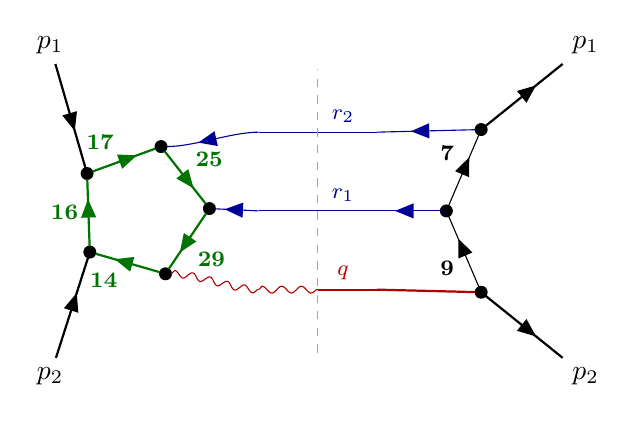
\begin{tikzpicture}
\begin{feynman}
\vertex (Lp1) at (-3.400,2.100) {$p_1$};
\vertex (Lp2) at (-3.400,-2.100) {$p_2$};
\vertex (Lcr1) at (-0.750,0.000);
\vertex (Lcr2) at (-0.750,1.000);
\vertex (Lcq) at (-0.750,-1.000);
\vertex (Mq) at (0,-1.000);
\vertex[dot] (Lv0) at (-1.934,-0.799) {};
\vertex[dot] (Lv1) at (-2.895,-0.523) {};
\vertex[dot] (Lv2) at (-2.930,0.475) {};
\vertex[dot] (Lv3) at (-1.991,0.817) {};
\vertex[dot] (Lv4) at (-1.376,0.030) {};
\vertex (Rp1) at (3.400,2.100) {$p_1$};
\vertex (Rp2) at (3.400,-2.100) {$p_2$};
\vertex (Rcr1) at (0.750,0.000);
\vertex (Rcr2) at (0.750,1.000);
\vertex (Rcq) at (0.750,-1.000);
\vertex[dot] (R7) at (2.075,1.033) {};
\vertex[dot] (R9) at (1.633,0.000) {};
\vertex[dot] (Rroot) at (2.075,-1.033) {};
\diagram* {
(Lv0) -- [plain, thick, green!45!black, with arrow=0.55, edge label={\footnotesize\bfseries 14}] (Lv1),
(Lv1) -- [plain, thick, green!45!black, with arrow=0.55, edge label={\footnotesize\bfseries 16}] (Lv2),
(Lv2) -- [plain, thick, green!45!black, with arrow=0.55, edge label={\footnotesize\bfseries 17}] (Lv3),
(Lv3) -- [plain, thick, green!45!black, with arrow=0.55, edge label={\footnotesize\bfseries 25}] (Lv4),
(Lv4) -- [plain, thick, green!45!black, with arrow=0.55, edge label={\footnotesize\bfseries 29}] (Lv0),
(Lcq) -- [boson, red!70!black, out=180, in=0, looseness=0.75] (Lv0),
(Lp2) -- [plain, thick, with arrow=0.55] (Lv1),
(Lp1) -- [plain, thick, with arrow=0.55] (Lv2),
(Lcr2) -- [plain, blue!60!black, out=180, in=0, looseness=0.75, with arrow=0.55] (Lv3),
(Lcr1) -- [plain, blue!60!black, with arrow=0.55] (Lv4),
(R9) -- [plain, with arrow=0.55, edge label={\footnotesize\bfseries 7}] (R7),
(Rroot) -- [plain, with arrow=0.55, edge label={\footnotesize\bfseries 9}] (R9),
(R7) -- [plain, thick, with arrow=0.55] (Rp1),
(Rroot) -- [plain, thick, with arrow=0.55] (Rp2),
(R9) -- [plain, blue!60!black, with arrow=0.55] (Rcr1),
(R7) -- [plain, blue!60!black, with arrow=0.55] (Rcr2),
(Rroot) -- [plain, red!70!black, double, double distance=1.2pt, thick] (Rcq),
(Rcr1) -- [plain, blue!60!black] (Lcr1),
(Rcr2) -- [plain, blue!60!black] (Lcr2),
(Rcq) -- [plain, red!70!black, double, double distance=1.2pt, thick] (Mq) -- [boson, red!70!black] (Lcq),
};
\end{feynman}
\draw[dashed, gray!70] (0,-1.80) -- (0,1.80);
\node[font=\footnotesize, blue!60!black, above] at (0.32,0.00) {$r_1$};
\node[font=\footnotesize, blue!60!black, above] at (0.32,1.00) {$r_2$};
\node[font=\footnotesize, red!70!black, above] at (0.32,-1.00) {$q$};
\end{tikzpicture}}\\[2mm]\textbf{topo1} (RR family 33, pentagon q-p2-p1-r2-r1)\\[2pt]{\footnotesize\begin{tabular}{@{}r@{\ \ }l@{\ \ }l@{}}\textbf{14} & $(k_1)^2$ & loop\\
\textbf{16} & $(k_1+p_2)^2$ & loop\\
\textbf{17} & $(k_1+p_1+p_2)^2$ & loop\\
\textbf{25} & $(k_1+p_1+p_2+r_2)^2$ & loop\\
\textbf{29} & $(k_1+p_1+p_2+r_1+r_2)^2$ & loop\\
\textbf{7} & $(p_1+r_2)^2$ & conjugate\\
\textbf{9} & $(p_1+r_1+r_2)^2$ & conjugate\\
\textbf{13} & $(p_1+p_2+r_2)^2$ & \textcolor{red}{irreducible numerator}\\\end{tabular}}\end{minipage}\hfill%
\begin{minipage}[t]{0.48\textwidth}\centering\resizebox{0.9\linewidth}{!}{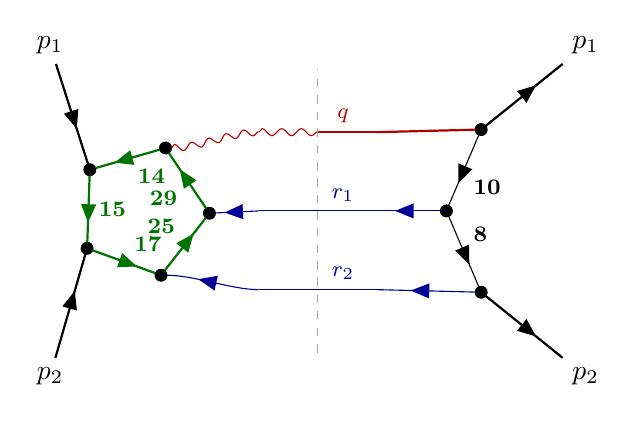
\begin{tikzpicture}
\begin{feynman}
\vertex (Lp1) at (-3.400,2.100) {$p_1$};
\vertex (Lp2) at (-3.400,-2.100) {$p_2$};
\vertex (Lcr1) at (-0.750,0.000);
\vertex (Lcr2) at (-0.750,-1.000);
\vertex (Lcq) at (-0.750,1.000);
\vertex (Mq) at (0,1.000);
\vertex[dot] (Lv0) at (-1.934,0.799) {};
\vertex[dot] (Lv1) at (-2.895,0.523) {};
\vertex[dot] (Lv2) at (-2.930,-0.475) {};
\vertex[dot] (Lv3) at (-1.991,-0.817) {};
\vertex[dot] (Lv4) at (-1.376,-0.030) {};
\vertex (Rp1) at (3.400,2.100) {$p_1$};
\vertex (Rp2) at (3.400,-2.100) {$p_2$};
\vertex (Rcr1) at (0.750,0.000);
\vertex (Rcr2) at (0.750,-1.000);
\vertex (Rcq) at (0.750,1.000);
\vertex[dot] (R8) at (2.075,-1.033) {};
\vertex[dot] (R10) at (1.633,0.000) {};
\vertex[dot] (Rroot) at (2.075,1.033) {};
\diagram* {
(Lv0) -- [plain, thick, green!45!black, with arrow=0.55, edge label={\footnotesize\bfseries 14}] (Lv1),
(Lv1) -- [plain, thick, green!45!black, with arrow=0.55, edge label={\footnotesize\bfseries 15}] (Lv2),
(Lv2) -- [plain, thick, green!45!black, with arrow=0.55, edge label={\footnotesize\bfseries 17}] (Lv3),
(Lv3) -- [plain, thick, green!45!black, with arrow=0.55, edge label={\footnotesize\bfseries 25}] (Lv4),
(Lv4) -- [plain, thick, green!45!black, with arrow=0.55, edge label={\footnotesize\bfseries 29}] (Lv0),
(Lcq) -- [boson, red!70!black, out=180, in=0, looseness=0.75] (Lv0),
(Lp1) -- [plain, thick, with arrow=0.55] (Lv1),
(Lp2) -- [plain, thick, with arrow=0.55] (Lv2),
(Lcr2) -- [plain, blue!60!black, out=180, in=0, looseness=0.75, with arrow=0.55] (Lv3),
(Lcr1) -- [plain, blue!60!black, with arrow=0.55] (Lv4),
(R10) -- [plain, with arrow=0.55, edge label={\footnotesize\bfseries 8}] (R8),
(Rroot) -- [plain, with arrow=0.55, edge label={\footnotesize\bfseries 10}] (R10),
(Rroot) -- [plain, thick, with arrow=0.55] (Rp1),
(R8) -- [plain, thick, with arrow=0.55] (Rp2),
(R10) -- [plain, blue!60!black, with arrow=0.55] (Rcr1),
(R8) -- [plain, blue!60!black, with arrow=0.55] (Rcr2),
(Rroot) -- [plain, red!70!black, double, double distance=1.2pt, thick] (Rcq),
(Rcr1) -- [plain, blue!60!black] (Lcr1),
(Rcr2) -- [plain, blue!60!black] (Lcr2),
(Rcq) -- [plain, red!70!black, double, double distance=1.2pt, thick] (Mq) -- [boson, red!70!black] (Lcq),
};
\end{feynman}
\draw[dashed, gray!70] (0,-1.80) -- (0,1.80);
\node[font=\footnotesize, blue!60!black, above] at (0.32,0.00) {$r_1$};
\node[font=\footnotesize, blue!60!black, above] at (0.32,-1.00) {$r_2$};
\node[font=\footnotesize, red!70!black, above] at (0.32,1.00) {$q$};
\end{tikzpicture}}\\[2mm]\textbf{topo2} (RR family 29, pentagon q-p1-p2-r2-r1)\\[2pt]{\footnotesize\begin{tabular}{@{}r@{\ \ }l@{\ \ }l@{}}\textbf{14} & $(k_1)^2$ & loop\\
\textbf{15} & $(k_1+p_1)^2$ & loop\\
\textbf{17} & $(k_1+p_1+p_2)^2$ & loop\\
\textbf{25} & $(k_1+p_1+p_2+r_2)^2$ & loop\\
\textbf{29} & $(k_1+p_1+p_2+r_1+r_2)^2$ & loop\\
\textbf{8} & $(p_2+r_2)^2$ & conjugate\\
\textbf{10} & $(p_2+r_1+r_2)^2$ & conjugate\\
\textbf{13} & $(p_1+p_2+r_2)^2$ & \textcolor{red}{irreducible numerator}\\\end{tabular}}\end{minipage}

\bigskip

\begin{minipage}[t]{0.48\textwidth}\centering\resizebox{0.9\linewidth}{!}{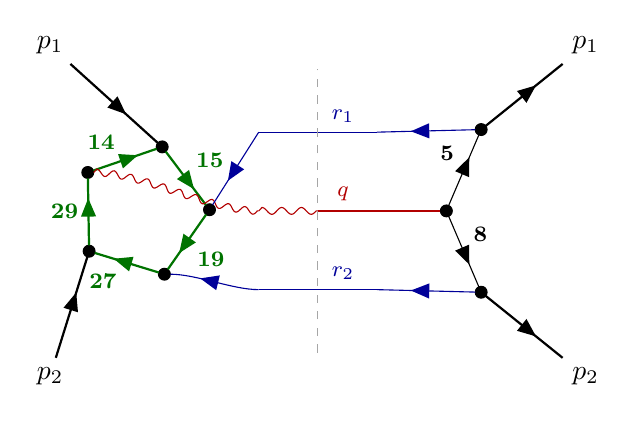
\begin{tikzpicture}
\begin{feynman}
\vertex (Lp1) at (-3.400,2.100) {$p_1$};
\vertex (Lp2) at (-3.400,-2.100) {$p_2$};
\vertex (Lcr1) at (-0.750,1.000);
\vertex (Lcr2) at (-0.750,-1.000);
\vertex (Lcq) at (-0.750,0.000);
\vertex (Mq) at (0,0.000);
\vertex[dot] (Lv0) at (-2.921,0.488) {};
\vertex[dot] (Lv1) at (-1.976,0.813) {};
\vertex[dot] (Lv2) at (-1.375,0.015) {};
\vertex[dot] (Lv3) at (-1.948,-0.804) {};
\vertex[dot] (Lv4) at (-2.904,-0.512) {};
\vertex (Rp1) at (3.400,2.100) {$p_1$};
\vertex (Rp2) at (3.400,-2.100) {$p_2$};
\vertex (Rcr1) at (0.750,1.000);
\vertex (Rcr2) at (0.750,-1.000);
\vertex (Rcq) at (0.750,0.000);
\vertex[dot] (R5) at (2.075,1.033) {};
\vertex[dot] (Rroot) at (1.633,0.000) {};
\vertex[dot] (R8) at (2.075,-1.033) {};
\diagram* {
(Lv0) -- [plain, thick, green!45!black, with arrow=0.55, edge label={\footnotesize\bfseries 14}] (Lv1),
(Lv1) -- [plain, thick, green!45!black, with arrow=0.55, edge label={\footnotesize\bfseries 15}] (Lv2),
(Lv2) -- [plain, thick, green!45!black, with arrow=0.55, edge label={\footnotesize\bfseries 19}] (Lv3),
(Lv3) -- [plain, thick, green!45!black, with arrow=0.55, edge label={\footnotesize\bfseries 27}] (Lv4),
(Lv4) -- [plain, thick, green!45!black, with arrow=0.55, edge label={\footnotesize\bfseries 29}] (Lv0),
(Lcq) -- [boson, red!70!black, out=180, in=0, looseness=0.75] (Lv0),
(Lp1) -- [plain, thick, with arrow=0.55] (Lv1),
(Lcr1) -- [plain, blue!60!black, with arrow=0.55] (Lv2),
(Lcr2) -- [plain, blue!60!black, out=180, in=0, looseness=0.75, with arrow=0.55] (Lv3),
(Lp2) -- [plain, thick, with arrow=0.55] (Lv4),
(Rroot) -- [plain, with arrow=0.55, edge label={\footnotesize\bfseries 5}] (R5),
(Rroot) -- [plain, with arrow=0.55, edge label={\footnotesize\bfseries 8}] (R8),
(R5) -- [plain, thick, with arrow=0.55] (Rp1),
(R8) -- [plain, thick, with arrow=0.55] (Rp2),
(R5) -- [plain, blue!60!black, with arrow=0.55] (Rcr1),
(R8) -- [plain, blue!60!black, with arrow=0.55] (Rcr2),
(Rroot) -- [plain, red!70!black, double, double distance=1.2pt, thick] (Rcq),
(Rcr1) -- [plain, blue!60!black] (Lcr1),
(Rcr2) -- [plain, blue!60!black] (Lcr2),
(Rcq) -- [plain, red!70!black, double, double distance=1.2pt, thick] (Mq) -- [boson, red!70!black] (Lcq),
};
\end{feynman}
\draw[dashed, gray!70] (0,-1.80) -- (0,1.80);
\node[font=\footnotesize, blue!60!black, above] at (0.32,1.00) {$r_1$};
\node[font=\footnotesize, blue!60!black, above] at (0.32,-1.00) {$r_2$};
\node[font=\footnotesize, red!70!black, above] at (0.32,0.00) {$q$};
\end{tikzpicture}}\\[2mm]\textbf{topo3} (RR family 8, pentagon q-p1-r1-r2-p2)\\[2pt]{\footnotesize\begin{tabular}{@{}r@{\ \ }l@{\ \ }l@{}}\textbf{14} & $(k_1)^2$ & loop\\
\textbf{15} & $(k_1+p_1)^2$ & loop\\
\textbf{19} & $(k_1+p_1+r_1)^2$ & loop\\
\textbf{27} & $(k_1+p_1+r_1+r_2)^2$ & loop\\
\textbf{29} & $(k_1+p_1+p_2+r_1+r_2)^2$ & loop\\
\textbf{5} & $(p_1+r_1)^2$ & conjugate\\
\textbf{8} & $(p_2+r_2)^2$ & conjugate\\
\textbf{11} & $(r_1+r_2)^2$ & \textcolor{red}{irreducible numerator}\\\end{tabular}}\end{minipage}\hfill%
\begin{minipage}[t]{0.48\textwidth}\centering\resizebox{0.9\linewidth}{!}{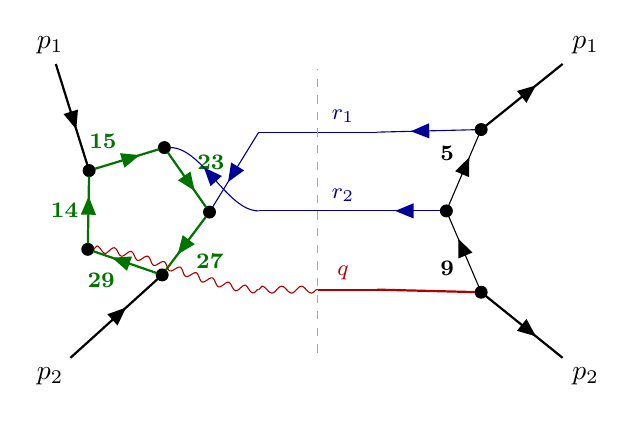
\begin{tikzpicture}
\begin{feynman}
\vertex (Lp1) at (-3.400,2.100) {$p_1$};
\vertex (Lp2) at (-3.400,-2.100) {$p_2$};
\vertex (Lcr1) at (-0.750,1.000);
\vertex (Lcr2) at (-0.750,0.000);
\vertex (Lcq) at (-0.750,-1.000);
\vertex (Mq) at (0,-1.000);
\vertex[dot] (Lv0) at (-2.921,-0.488) {};
\vertex[dot] (Lv1) at (-2.904,0.512) {};
\vertex[dot] (Lv2) at (-1.948,0.804) {};
\vertex[dot] (Lv3) at (-1.375,-0.015) {};
\vertex[dot] (Lv4) at (-1.976,-0.813) {};
\vertex (Rp1) at (3.400,2.100) {$p_1$};
\vertex (Rp2) at (3.400,-2.100) {$p_2$};
\vertex (Rcr1) at (0.750,1.000);
\vertex (Rcr2) at (0.750,0.000);
\vertex (Rcq) at (0.750,-1.000);
\vertex[dot] (R5) at (2.075,1.033) {};
\vertex[dot] (R9) at (1.633,0.000) {};
\vertex[dot] (Rroot) at (2.075,-1.033) {};
\diagram* {
(Lv0) -- [plain, thick, green!45!black, with arrow=0.55, edge label={\footnotesize\bfseries 14}] (Lv1),
(Lv1) -- [plain, thick, green!45!black, with arrow=0.55, edge label={\footnotesize\bfseries 15}] (Lv2),
(Lv2) -- [plain, thick, green!45!black, with arrow=0.55, edge label={\footnotesize\bfseries 23}] (Lv3),
(Lv3) -- [plain, thick, green!45!black, with arrow=0.55, edge label={\footnotesize\bfseries 27}] (Lv4),
(Lv4) -- [plain, thick, green!45!black, with arrow=0.55, edge label={\footnotesize\bfseries 29}] (Lv0),
(Lcq) -- [boson, red!70!black, out=180, in=0, looseness=0.75] (Lv0),
(Lp1) -- [plain, thick, with arrow=0.55] (Lv1),
(Lcr2) -- [plain, blue!60!black, out=180, in=0, looseness=0.75, with arrow=0.55] (Lv2),
(Lcr1) -- [plain, blue!60!black, with arrow=0.55] (Lv3),
(Lp2) -- [plain, thick, with arrow=0.55] (Lv4),
(R9) -- [plain, with arrow=0.55, edge label={\footnotesize\bfseries 5}] (R5),
(Rroot) -- [plain, with arrow=0.55, edge label={\footnotesize\bfseries 9}] (R9),
(R5) -- [plain, thick, with arrow=0.55] (Rp1),
(Rroot) -- [plain, thick, with arrow=0.55] (Rp2),
(R5) -- [plain, blue!60!black, with arrow=0.55] (Rcr1),
(R9) -- [plain, blue!60!black, with arrow=0.55] (Rcr2),
(Rroot) -- [plain, red!70!black, double, double distance=1.2pt, thick] (Rcq),
(Rcr1) -- [plain, blue!60!black] (Lcr1),
(Rcr2) -- [plain, blue!60!black] (Lcr2),
(Rcq) -- [plain, red!70!black, double, double distance=1.2pt, thick] (Mq) -- [boson, red!70!black] (Lcq),
};
\end{feynman}
\draw[dashed, gray!70] (0,-1.80) -- (0,1.80);
\node[font=\footnotesize, blue!60!black, above] at (0.32,1.00) {$r_1$};
\node[font=\footnotesize, blue!60!black, above] at (0.32,0.00) {$r_2$};
\node[font=\footnotesize, red!70!black, above] at (0.32,-1.00) {$q$};
\end{tikzpicture}}\\[2mm]\textbf{topo4} (RR family 3, pentagon q-p1-r2-r1-p2)\\[2pt]{\footnotesize\begin{tabular}{@{}r@{\ \ }l@{\ \ }l@{}}\textbf{14} & $(k_1)^2$ & loop\\
\textbf{15} & $(k_1+p_1)^2$ & loop\\
\textbf{23} & $(k_1+p_1+r_2)^2$ & loop\\
\textbf{27} & $(k_1+p_1+r_1+r_2)^2$ & loop\\
\textbf{29} & $(k_1+p_1+p_2+r_1+r_2)^2$ & loop\\
\textbf{5} & $(p_1+r_1)^2$ & conjugate\\
\textbf{9} & $(p_1+r_1+r_2)^2$ & conjugate\\
\textbf{6} & $(p_2+r_1)^2$ & \textcolor{red}{irreducible numerator}\\\end{tabular}}\end{minipage}

\bigskip

\begin{minipage}[t]{0.48\textwidth}\centering\resizebox{0.9\linewidth}{!}{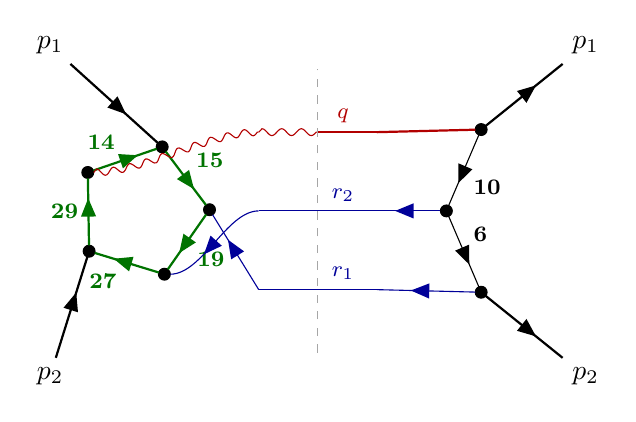
\begin{tikzpicture}
\begin{feynman}
\vertex (Lp1) at (-3.400,2.100) {$p_1$};
\vertex (Lp2) at (-3.400,-2.100) {$p_2$};
\vertex (Lcr1) at (-0.750,-1.000);
\vertex (Lcr2) at (-0.750,0.000);
\vertex (Lcq) at (-0.750,1.000);
\vertex (Mq) at (0,1.000);
\vertex[dot] (Lv0) at (-2.921,0.488) {};
\vertex[dot] (Lv1) at (-1.976,0.813) {};
\vertex[dot] (Lv2) at (-1.375,0.015) {};
\vertex[dot] (Lv3) at (-1.948,-0.804) {};
\vertex[dot] (Lv4) at (-2.904,-0.512) {};
\vertex (Rp1) at (3.400,2.100) {$p_1$};
\vertex (Rp2) at (3.400,-2.100) {$p_2$};
\vertex (Rcr1) at (0.750,-1.000);
\vertex (Rcr2) at (0.750,0.000);
\vertex (Rcq) at (0.750,1.000);
\vertex[dot] (R6) at (2.075,-1.033) {};
\vertex[dot] (R10) at (1.633,0.000) {};
\vertex[dot] (Rroot) at (2.075,1.033) {};
\diagram* {
(Lv0) -- [plain, thick, green!45!black, with arrow=0.55, edge label={\footnotesize\bfseries 14}] (Lv1),
(Lv1) -- [plain, thick, green!45!black, with arrow=0.55, edge label={\footnotesize\bfseries 15}] (Lv2),
(Lv2) -- [plain, thick, green!45!black, with arrow=0.55, edge label={\footnotesize\bfseries 19}] (Lv3),
(Lv3) -- [plain, thick, green!45!black, with arrow=0.55, edge label={\footnotesize\bfseries 27}] (Lv4),
(Lv4) -- [plain, thick, green!45!black, with arrow=0.55, edge label={\footnotesize\bfseries 29}] (Lv0),
(Lcq) -- [boson, red!70!black, out=180, in=0, looseness=0.75] (Lv0),
(Lp1) -- [plain, thick, with arrow=0.55] (Lv1),
(Lcr1) -- [plain, blue!60!black, with arrow=0.55] (Lv2),
(Lcr2) -- [plain, blue!60!black, out=180, in=0, looseness=0.75, with arrow=0.55] (Lv3),
(Lp2) -- [plain, thick, with arrow=0.55] (Lv4),
(R10) -- [plain, with arrow=0.55, edge label={\footnotesize\bfseries 6}] (R6),
(Rroot) -- [plain, with arrow=0.55, edge label={\footnotesize\bfseries 10}] (R10),
(Rroot) -- [plain, thick, with arrow=0.55] (Rp1),
(R6) -- [plain, thick, with arrow=0.55] (Rp2),
(R6) -- [plain, blue!60!black, with arrow=0.55] (Rcr1),
(R10) -- [plain, blue!60!black, with arrow=0.55] (Rcr2),
(Rroot) -- [plain, red!70!black, double, double distance=1.2pt, thick] (Rcq),
(Rcr1) -- [plain, blue!60!black] (Lcr1),
(Rcr2) -- [plain, blue!60!black] (Lcr2),
(Rcq) -- [plain, red!70!black, double, double distance=1.2pt, thick] (Mq) -- [boson, red!70!black] (Lcq),
};
\end{feynman}
\draw[dashed, gray!70] (0,-1.80) -- (0,1.80);
\node[font=\footnotesize, blue!60!black, above] at (0.32,-1.00) {$r_1$};
\node[font=\footnotesize, blue!60!black, above] at (0.32,0.00) {$r_2$};
\node[font=\footnotesize, red!70!black, above] at (0.32,1.00) {$q$};
\end{tikzpicture}}\\[2mm]\textbf{topo5} (RR family 4, pentagon q-p1-r1-r2-p2)\\[2pt]{\footnotesize\begin{tabular}{@{}r@{\ \ }l@{\ \ }l@{}}\textbf{14} & $(k_1)^2$ & loop\\
\textbf{15} & $(k_1+p_1)^2$ & loop\\
\textbf{19} & $(k_1+p_1+r_1)^2$ & loop\\
\textbf{27} & $(k_1+p_1+r_1+r_2)^2$ & loop\\
\textbf{29} & $(k_1+p_1+p_2+r_1+r_2)^2$ & loop\\
\textbf{6} & $(p_2+r_1)^2$ & conjugate\\
\textbf{10} & $(p_2+r_1+r_2)^2$ & conjugate\\
\textbf{5} & $(p_1+r_1)^2$ & \textcolor{red}{irreducible numerator}\\\end{tabular}}\end{minipage}\hfill%
\begin{minipage}[t]{0.48\textwidth}\centering\resizebox{0.9\linewidth}{!}{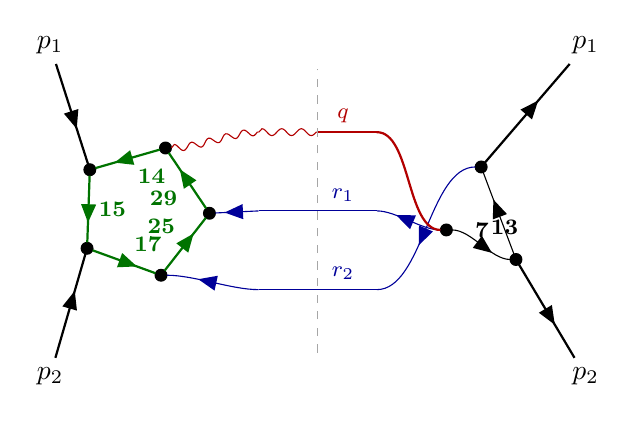
\begin{tikzpicture}
\begin{feynman}
\vertex (Lp1) at (-3.400,2.100) {$p_1$};
\vertex (Lp2) at (-3.400,-2.100) {$p_2$};
\vertex (Lcr1) at (-0.750,0.000);
\vertex (Lcr2) at (-0.750,-1.000);
\vertex (Lcq) at (-0.750,1.000);
\vertex (Mq) at (0,1.000);
\vertex[dot] (Lv0) at (-1.934,0.799) {};
\vertex[dot] (Lv1) at (-2.895,0.523) {};
\vertex[dot] (Lv2) at (-2.930,-0.475) {};
\vertex[dot] (Lv3) at (-1.991,-0.817) {};
\vertex[dot] (Lv4) at (-1.376,-0.030) {};
\vertex (Rp1) at (3.400,2.100) {$p_1$};
\vertex (Rp2) at (3.400,-2.100) {$p_2$};
\vertex (Rcr1) at (0.750,0.000);
\vertex (Rcr2) at (0.750,-1.000);
\vertex (Rcq) at (0.750,1.000);
\vertex[dot] (R7) at (2.075,0.558) {};
\vertex[dot] (R13) at (2.517,-0.617) {};
\vertex[dot] (Rroot) at (1.633,-0.242) {};
\diagram* {
(Lv0) -- [plain, thick, green!45!black, with arrow=0.55, edge label={\footnotesize\bfseries 14}] (Lv1),
(Lv1) -- [plain, thick, green!45!black, with arrow=0.55, edge label={\footnotesize\bfseries 15}] (Lv2),
(Lv2) -- [plain, thick, green!45!black, with arrow=0.55, edge label={\footnotesize\bfseries 17}] (Lv3),
(Lv3) -- [plain, thick, green!45!black, with arrow=0.55, edge label={\footnotesize\bfseries 25}] (Lv4),
(Lv4) -- [plain, thick, green!45!black, with arrow=0.55, edge label={\footnotesize\bfseries 29}] (Lv0),
(Lcq) -- [boson, red!70!black, out=180, in=0, looseness=0.75] (Lv0),
(Lp1) -- [plain, thick, with arrow=0.55] (Lv1),
(Lp2) -- [plain, thick, with arrow=0.55] (Lv2),
(Lcr2) -- [plain, blue!60!black, out=180, in=0, looseness=0.75, with arrow=0.55] (Lv3),
(Lcr1) -- [plain, blue!60!black, with arrow=0.55] (Lv4),
(R13) -- [plain, with arrow=0.55, edge label={\footnotesize\bfseries 7}] (R7),
(Rroot) -- [plain, out=0, in=180, looseness=0.75, with arrow=0.55, edge label={\footnotesize\bfseries 13}] (R13),
(R7) -- [plain, thick, with arrow=0.55] (Rp1),
(R13) -- [plain, thick, with arrow=0.55] (Rp2),
(Rroot) -- [plain, blue!60!black, out=180, in=0, looseness=0.75, with arrow=0.55] (Rcr1),
(R7) -- [plain, blue!60!black, out=180, in=0, looseness=0.75, with arrow=0.55] (Rcr2),
(Rroot) -- [plain, red!70!black, double, double distance=1.2pt, thick, out=180, in=0, looseness=0.75] (Rcq),
(Rcr1) -- [plain, blue!60!black] (Lcr1),
(Rcr2) -- [plain, blue!60!black] (Lcr2),
(Rcq) -- [plain, red!70!black, double, double distance=1.2pt, thick] (Mq) -- [boson, red!70!black] (Lcq),
};
\end{feynman}
\draw[dashed, gray!70] (0,-1.80) -- (0,1.80);
\node[font=\footnotesize, blue!60!black, above] at (0.32,0.00) {$r_1$};
\node[font=\footnotesize, blue!60!black, above] at (0.32,-1.00) {$r_2$};
\node[font=\footnotesize, red!70!black, above] at (0.32,1.00) {$q$};
\end{tikzpicture}}\\[2mm]\textbf{topo6} (RR family 30, pentagon q-p1-p2-r2-r1)\\[2pt]{\footnotesize\begin{tabular}{@{}r@{\ \ }l@{\ \ }l@{}}\textbf{14} & $(k_1)^2$ & loop\\
\textbf{15} & $(k_1+p_1)^2$ & loop\\
\textbf{17} & $(k_1+p_1+p_2)^2$ & loop\\
\textbf{25} & $(k_1+p_1+p_2+r_2)^2$ & loop\\
\textbf{29} & $(k_1+p_1+p_2+r_1+r_2)^2$ & loop\\
\textbf{7} & $(p_1+r_2)^2$ & conjugate\\
\textbf{13} & $(p_1+p_2+r_2)^2$ & conjugate\\
\textbf{11} & $(r_1+r_2)^2$ & \textcolor{red}{irreducible numerator}\\\end{tabular}}\end{minipage}

\bigskip

\begin{minipage}[t]{0.48\textwidth}\centering\resizebox{0.9\linewidth}{!}{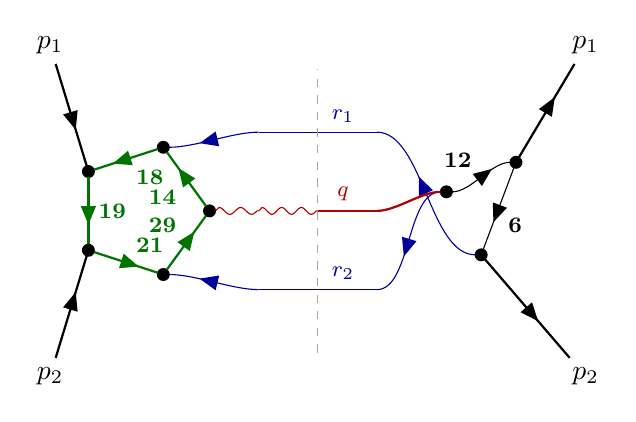
\begin{tikzpicture}
\begin{feynman}
\vertex (Lp1) at (-3.400,2.100) {$p_1$};
\vertex (Lp2) at (-3.400,-2.100) {$p_2$};
\vertex (Lcr1) at (-0.750,1.000);
\vertex (Lcr2) at (-0.750,-1.000);
\vertex (Lcq) at (-0.750,0.000);
\vertex (Mq) at (0,0.000);
\vertex[dot] (Lv0) at (-1.375,0.000) {};
\vertex[dot] (Lv1) at (-1.962,0.808) {};
\vertex[dot] (Lv2) at (-2.913,0.500) {};
\vertex[dot] (Lv3) at (-2.913,-0.500) {};
\vertex[dot] (Lv4) at (-1.962,-0.808) {};
\vertex (Rp1) at (3.400,2.100) {$p_1$};
\vertex (Rp2) at (3.400,-2.100) {$p_2$};
\vertex (Rcr1) at (0.750,1.000);
\vertex (Rcr2) at (0.750,-1.000);
\vertex (Rcq) at (0.750,0.000);
\vertex[dot] (R6) at (2.075,-0.558) {};
\vertex[dot] (R12) at (2.517,0.617) {};
\vertex[dot] (Rroot) at (1.633,0.242) {};
\diagram* {
(Lv0) -- [plain, thick, green!45!black, with arrow=0.55, edge label={\footnotesize\bfseries 14}] (Lv1),
(Lv1) -- [plain, thick, green!45!black, with arrow=0.55, edge label={\footnotesize\bfseries 18}] (Lv2),
(Lv2) -- [plain, thick, green!45!black, with arrow=0.55, edge label={\footnotesize\bfseries 19}] (Lv3),
(Lv3) -- [plain, thick, green!45!black, with arrow=0.55, edge label={\footnotesize\bfseries 21}] (Lv4),
(Lv4) -- [plain, thick, green!45!black, with arrow=0.55, edge label={\footnotesize\bfseries 29}] (Lv0),
(Lcq) -- [boson, red!70!black] (Lv0),
(Lcr1) -- [plain, blue!60!black, out=180, in=0, looseness=0.75, with arrow=0.55] (Lv1),
(Lp1) -- [plain, thick, with arrow=0.55] (Lv2),
(Lp2) -- [plain, thick, with arrow=0.55] (Lv3),
(Lcr2) -- [plain, blue!60!black, out=180, in=0, looseness=0.75, with arrow=0.55] (Lv4),
(R12) -- [plain, with arrow=0.55, edge label={\footnotesize\bfseries 6}] (R6),
(Rroot) -- [plain, out=0, in=180, looseness=0.75, with arrow=0.55, edge label={\footnotesize\bfseries 12}] (R12),
(R12) -- [plain, thick, with arrow=0.55] (Rp1),
(R6) -- [plain, thick, with arrow=0.55] (Rp2),
(R6) -- [plain, blue!60!black, out=180, in=0, looseness=0.75, with arrow=0.55] (Rcr1),
(Rroot) -- [plain, blue!60!black, out=180, in=0, looseness=0.75, with arrow=0.55] (Rcr2),
(Rroot) -- [plain, red!70!black, double, double distance=1.2pt, thick, out=180, in=0, looseness=0.75] (Rcq),
(Rcr1) -- [plain, blue!60!black] (Lcr1),
(Rcr2) -- [plain, blue!60!black] (Lcr2),
(Rcq) -- [plain, red!70!black, double, double distance=1.2pt, thick] (Mq) -- [boson, red!70!black] (Lcq),
};
\end{feynman}
\draw[dashed, gray!70] (0,-1.80) -- (0,1.80);
\node[font=\footnotesize, blue!60!black, above] at (0.32,1.00) {$r_1$};
\node[font=\footnotesize, blue!60!black, above] at (0.32,-1.00) {$r_2$};
\node[font=\footnotesize, red!70!black, above] at (0.32,0.00) {$q$};
\end{tikzpicture}}\\[2mm]\textbf{topo7} (RR family 24, pentagon q-r1-p1-p2-r2)\\[2pt]{\footnotesize\begin{tabular}{@{}r@{\ \ }l@{\ \ }l@{}}\textbf{14} & $(k_1)^2$ & loop\\
\textbf{18} & $(k_1+r_1)^2$ & loop\\
\textbf{19} & $(k_1+p_1+r_1)^2$ & loop\\
\textbf{21} & $(k_1+p_1+p_2+r_1)^2$ & loop\\
\textbf{29} & $(k_1+p_1+p_2+r_1+r_2)^2$ & loop\\
\textbf{6} & $(p_2+r_1)^2$ & conjugate\\
\textbf{12} & $(p_1+p_2+r_1)^2$ & conjugate\\
\textbf{13} & $(p_1+p_2+r_2)^2$ & \textcolor{red}{irreducible numerator}\\\end{tabular}}\end{minipage}\hfill%
\begin{minipage}[t]{0.48\textwidth}\centering\resizebox{0.9\linewidth}{!}{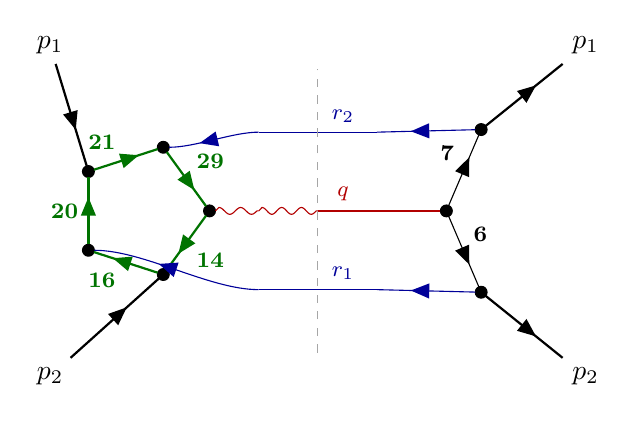
\begin{tikzpicture}
\begin{feynman}
\vertex (Lp1) at (-3.400,2.100) {$p_1$};
\vertex (Lp2) at (-3.400,-2.100) {$p_2$};
\vertex (Lcr1) at (-0.750,-1.000);
\vertex (Lcr2) at (-0.750,1.000);
\vertex (Lcq) at (-0.750,0.000);
\vertex (Mq) at (0,0.000);
\vertex[dot] (Lv0) at (-1.375,0.000) {};
\vertex[dot] (Lv1) at (-1.962,-0.808) {};
\vertex[dot] (Lv2) at (-2.913,-0.500) {};
\vertex[dot] (Lv3) at (-2.913,0.500) {};
\vertex[dot] (Lv4) at (-1.962,0.808) {};
\vertex (Rp1) at (3.400,2.100) {$p_1$};
\vertex (Rp2) at (3.400,-2.100) {$p_2$};
\vertex (Rcr1) at (0.750,-1.000);
\vertex (Rcr2) at (0.750,1.000);
\vertex (Rcq) at (0.750,0.000);
\vertex[dot] (R6) at (2.075,-1.033) {};
\vertex[dot] (Rroot) at (1.633,0.000) {};
\vertex[dot] (R7) at (2.075,1.033) {};
\diagram* {
(Lv0) -- [plain, thick, green!45!black, with arrow=0.55, edge label={\footnotesize\bfseries 14}] (Lv1),
(Lv1) -- [plain, thick, green!45!black, with arrow=0.55, edge label={\footnotesize\bfseries 16}] (Lv2),
(Lv2) -- [plain, thick, green!45!black, with arrow=0.55, edge label={\footnotesize\bfseries 20}] (Lv3),
(Lv3) -- [plain, thick, green!45!black, with arrow=0.55, edge label={\footnotesize\bfseries 21}] (Lv4),
(Lv4) -- [plain, thick, green!45!black, with arrow=0.55, edge label={\footnotesize\bfseries 29}] (Lv0),
(Lcq) -- [boson, red!70!black] (Lv0),
(Lp2) -- [plain, thick, with arrow=0.55] (Lv1),
(Lcr1) -- [plain, blue!60!black, out=180, in=0, looseness=0.75, with arrow=0.55] (Lv2),
(Lp1) -- [plain, thick, with arrow=0.55] (Lv3),
(Lcr2) -- [plain, blue!60!black, out=180, in=0, looseness=0.75, with arrow=0.55] (Lv4),
(Rroot) -- [plain, with arrow=0.55, edge label={\footnotesize\bfseries 6}] (R6),
(Rroot) -- [plain, with arrow=0.55, edge label={\footnotesize\bfseries 7}] (R7),
(R7) -- [plain, thick, with arrow=0.55] (Rp1),
(R6) -- [plain, thick, with arrow=0.55] (Rp2),
(R6) -- [plain, blue!60!black, with arrow=0.55] (Rcr1),
(R7) -- [plain, blue!60!black, with arrow=0.55] (Rcr2),
(Rroot) -- [plain, red!70!black, double, double distance=1.2pt, thick] (Rcq),
(Rcr1) -- [plain, blue!60!black] (Lcr1),
(Rcr2) -- [plain, blue!60!black] (Lcr2),
(Rcq) -- [plain, red!70!black, double, double distance=1.2pt, thick] (Mq) -- [boson, red!70!black] (Lcq),
};
\end{feynman}
\draw[dashed, gray!70] (0,-1.80) -- (0,1.80);
\node[font=\footnotesize, blue!60!black, above] at (0.32,-1.00) {$r_1$};
\node[font=\footnotesize, blue!60!black, above] at (0.32,1.00) {$r_2$};
\node[font=\footnotesize, red!70!black, above] at (0.32,0.00) {$q$};
\end{tikzpicture}}\\[2mm]\textbf{topo8} (RR family 1, pentagon q-p2-r1-p1-r2)\\[2pt]{\footnotesize\begin{tabular}{@{}r@{\ \ }l@{\ \ }l@{}}\textbf{14} & $(k_1)^2$ & loop\\
\textbf{16} & $(k_1+p_2)^2$ & loop\\
\textbf{20} & $(k_1+p_2+r_1)^2$ & loop\\
\textbf{21} & $(k_1+p_1+p_2+r_1)^2$ & loop\\
\textbf{29} & $(k_1+p_1+p_2+r_1+r_2)^2$ & loop\\
\textbf{6} & $(p_2+r_1)^2$ & conjugate\\
\textbf{7} & $(p_1+r_2)^2$ & conjugate\\
\textbf{5} & $(p_1+r_1)^2$ & \textcolor{red}{irreducible numerator}\\\end{tabular}}\end{minipage}

\bigskip

\begin{minipage}[t]{0.48\textwidth}\centering\resizebox{0.9\linewidth}{!}{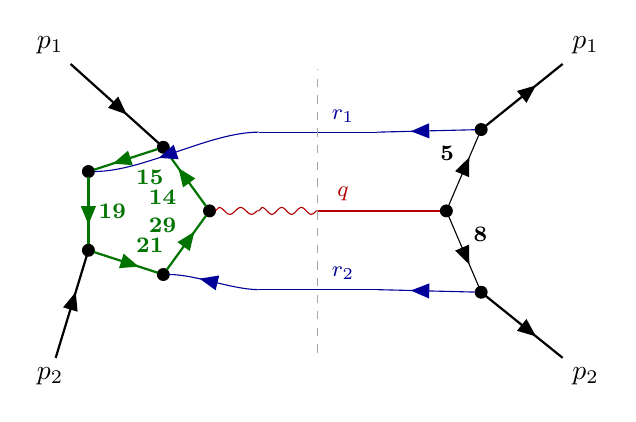
\begin{tikzpicture}
\begin{feynman}
\vertex (Lp1) at (-3.400,2.100) {$p_1$};
\vertex (Lp2) at (-3.400,-2.100) {$p_2$};
\vertex (Lcr1) at (-0.750,1.000);
\vertex (Lcr2) at (-0.750,-1.000);
\vertex (Lcq) at (-0.750,0.000);
\vertex (Mq) at (0,0.000);
\vertex[dot] (Lv0) at (-1.375,0.000) {};
\vertex[dot] (Lv1) at (-1.962,0.808) {};
\vertex[dot] (Lv2) at (-2.913,0.500) {};
\vertex[dot] (Lv3) at (-2.913,-0.500) {};
\vertex[dot] (Lv4) at (-1.962,-0.808) {};
\vertex (Rp1) at (3.400,2.100) {$p_1$};
\vertex (Rp2) at (3.400,-2.100) {$p_2$};
\vertex (Rcr1) at (0.750,1.000);
\vertex (Rcr2) at (0.750,-1.000);
\vertex (Rcq) at (0.750,0.000);
\vertex[dot] (R5) at (2.075,1.033) {};
\vertex[dot] (Rroot) at (1.633,0.000) {};
\vertex[dot] (R8) at (2.075,-1.033) {};
\diagram* {
(Lv0) -- [plain, thick, green!45!black, with arrow=0.55, edge label={\footnotesize\bfseries 14}] (Lv1),
(Lv1) -- [plain, thick, green!45!black, with arrow=0.55, edge label={\footnotesize\bfseries 15}] (Lv2),
(Lv2) -- [plain, thick, green!45!black, with arrow=0.55, edge label={\footnotesize\bfseries 19}] (Lv3),
(Lv3) -- [plain, thick, green!45!black, with arrow=0.55, edge label={\footnotesize\bfseries 21}] (Lv4),
(Lv4) -- [plain, thick, green!45!black, with arrow=0.55, edge label={\footnotesize\bfseries 29}] (Lv0),
(Lcq) -- [boson, red!70!black] (Lv0),
(Lp1) -- [plain, thick, with arrow=0.55] (Lv1),
(Lcr1) -- [plain, blue!60!black, out=180, in=0, looseness=0.75, with arrow=0.55] (Lv2),
(Lp2) -- [plain, thick, with arrow=0.55] (Lv3),
(Lcr2) -- [plain, blue!60!black, out=180, in=0, looseness=0.75, with arrow=0.55] (Lv4),
(Rroot) -- [plain, with arrow=0.55, edge label={\footnotesize\bfseries 5}] (R5),
(Rroot) -- [plain, with arrow=0.55, edge label={\footnotesize\bfseries 8}] (R8),
(R5) -- [plain, thick, with arrow=0.55] (Rp1),
(R8) -- [plain, thick, with arrow=0.55] (Rp2),
(R5) -- [plain, blue!60!black, with arrow=0.55] (Rcr1),
(R8) -- [plain, blue!60!black, with arrow=0.55] (Rcr2),
(Rroot) -- [plain, red!70!black, double, double distance=1.2pt, thick] (Rcq),
(Rcr1) -- [plain, blue!60!black] (Lcr1),
(Rcr2) -- [plain, blue!60!black] (Lcr2),
(Rcq) -- [plain, red!70!black, double, double distance=1.2pt, thick] (Mq) -- [boson, red!70!black] (Lcq),
};
\end{feynman}
\draw[dashed, gray!70] (0,-1.80) -- (0,1.80);
\node[font=\footnotesize, blue!60!black, above] at (0.32,1.00) {$r_1$};
\node[font=\footnotesize, blue!60!black, above] at (0.32,-1.00) {$r_2$};
\node[font=\footnotesize, red!70!black, above] at (0.32,0.00) {$q$};
\end{tikzpicture}}\\[2mm]\textbf{topo9} (RR family 7, pentagon q-p1-r1-p2-r2)\\[2pt]{\footnotesize\begin{tabular}{@{}r@{\ \ }l@{\ \ }l@{}}\textbf{14} & $(k_1)^2$ & loop\\
\textbf{15} & $(k_1+p_1)^2$ & loop\\
\textbf{19} & $(k_1+p_1+r_1)^2$ & loop\\
\textbf{21} & $(k_1+p_1+p_2+r_1)^2$ & loop\\
\textbf{29} & $(k_1+p_1+p_2+r_1+r_2)^2$ & loop\\
\textbf{5} & $(p_1+r_1)^2$ & conjugate\\
\textbf{8} & $(p_2+r_2)^2$ & conjugate\\
\textbf{10} & $(p_2+r_1+r_2)^2$ & \textcolor{red}{irreducible numerator}\\\end{tabular}}\end{minipage}\hfill%
\begin{minipage}[t]{0.48\textwidth}\centering\resizebox{0.9\linewidth}{!}{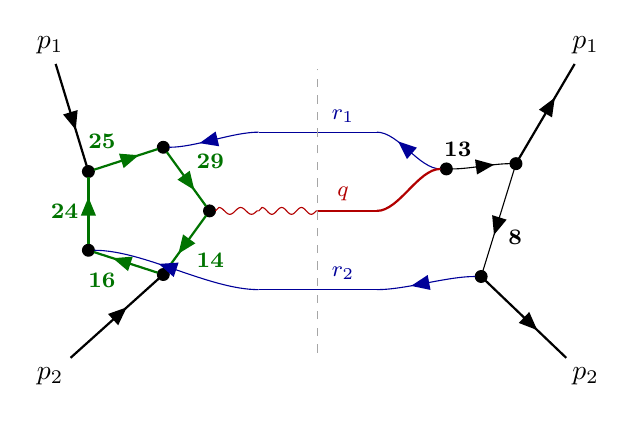
\begin{tikzpicture}
\begin{feynman}
\vertex (Lp1) at (-3.400,2.100) {$p_1$};
\vertex (Lp2) at (-3.400,-2.100) {$p_2$};
\vertex (Lcr1) at (-0.750,1.000);
\vertex (Lcr2) at (-0.750,-1.000);
\vertex (Lcq) at (-0.750,0.000);
\vertex (Mq) at (0,0.000);
\vertex[dot] (Lv0) at (-1.375,0.000) {};
\vertex[dot] (Lv1) at (-1.962,-0.808) {};
\vertex[dot] (Lv2) at (-2.913,-0.500) {};
\vertex[dot] (Lv3) at (-2.913,0.500) {};
\vertex[dot] (Lv4) at (-1.962,0.808) {};
\vertex (Rp1) at (3.400,2.100) {$p_1$};
\vertex (Rp2) at (3.400,-2.100) {$p_2$};
\vertex (Rcr1) at (0.750,1.000);
\vertex (Rcr2) at (0.750,-1.000);
\vertex (Rcq) at (0.750,0.000);
\vertex[dot] (R8) at (2.075,-0.833) {};
\vertex[dot] (R13) at (2.517,0.600) {};
\vertex[dot] (Rroot) at (1.633,0.533) {};
\diagram* {
(Lv0) -- [plain, thick, green!45!black, with arrow=0.55, edge label={\footnotesize\bfseries 14}] (Lv1),
(Lv1) -- [plain, thick, green!45!black, with arrow=0.55, edge label={\footnotesize\bfseries 16}] (Lv2),
(Lv2) -- [plain, thick, green!45!black, with arrow=0.55, edge label={\footnotesize\bfseries 24}] (Lv3),
(Lv3) -- [plain, thick, green!45!black, with arrow=0.55, edge label={\footnotesize\bfseries 25}] (Lv4),
(Lv4) -- [plain, thick, green!45!black, with arrow=0.55, edge label={\footnotesize\bfseries 29}] (Lv0),
(Lcq) -- [boson, red!70!black] (Lv0),
(Lp2) -- [plain, thick, with arrow=0.55] (Lv1),
(Lcr2) -- [plain, blue!60!black, out=180, in=0, looseness=0.75, with arrow=0.55] (Lv2),
(Lp1) -- [plain, thick, with arrow=0.55] (Lv3),
(Lcr1) -- [plain, blue!60!black, out=180, in=0, looseness=0.75, with arrow=0.55] (Lv4),
(R13) -- [plain, with arrow=0.55, edge label={\footnotesize\bfseries 8}] (R8),
(Rroot) -- [plain, out=0, in=180, looseness=0.75, with arrow=0.55, edge label={\footnotesize\bfseries 13}] (R13),
(R13) -- [plain, thick, with arrow=0.55] (Rp1),
(R8) -- [plain, thick, with arrow=0.55] (Rp2),
(Rroot) -- [plain, blue!60!black, out=180, in=0, looseness=0.75, with arrow=0.55] (Rcr1),
(R8) -- [plain, blue!60!black, out=180, in=0, looseness=0.75, with arrow=0.55] (Rcr2),
(Rroot) -- [plain, red!70!black, double, double distance=1.2pt, thick, out=180, in=0, looseness=0.75] (Rcq),
(Rcr1) -- [plain, blue!60!black] (Lcr1),
(Rcr2) -- [plain, blue!60!black] (Lcr2),
(Rcq) -- [plain, red!70!black, double, double distance=1.2pt, thick] (Mq) -- [boson, red!70!black] (Lcq),
};
\end{feynman}
\draw[dashed, gray!70] (0,-1.80) -- (0,1.80);
\node[font=\footnotesize, blue!60!black, above] at (0.32,1.00) {$r_1$};
\node[font=\footnotesize, blue!60!black, above] at (0.32,-1.00) {$r_2$};
\node[font=\footnotesize, red!70!black, above] at (0.32,0.00) {$q$};
\end{tikzpicture}}\\[2mm]\textbf{topo10} (RR family 34, pentagon q-p2-r2-p1-r1)\\[2pt]{\footnotesize\begin{tabular}{@{}r@{\ \ }l@{\ \ }l@{}}\textbf{14} & $(k_1)^2$ & loop\\
\textbf{16} & $(k_1+p_2)^2$ & loop\\
\textbf{24} & $(k_1+p_2+r_2)^2$ & loop\\
\textbf{25} & $(k_1+p_1+p_2+r_2)^2$ & loop\\
\textbf{29} & $(k_1+p_1+p_2+r_1+r_2)^2$ & loop\\
\textbf{8} & $(p_2+r_2)^2$ & conjugate\\
\textbf{13} & $(p_1+p_2+r_2)^2$ & conjugate\\
\textbf{9} & $(p_1+r_1+r_2)^2$ & \textcolor{red}{irreducible numerator}\\\end{tabular}}\end{minipage}

\bigskip

\begin{minipage}[t]{0.48\textwidth}\centering\resizebox{0.9\linewidth}{!}{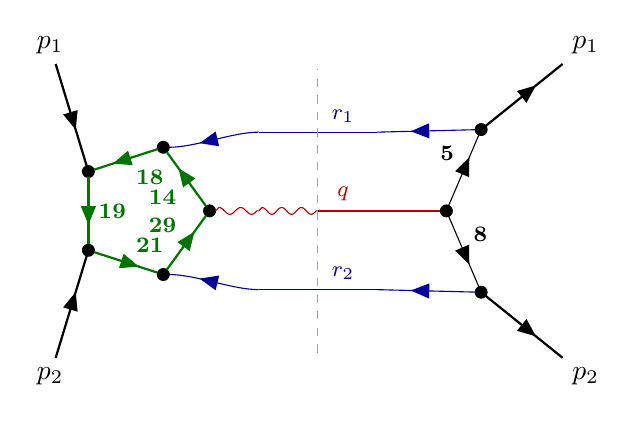
\begin{tikzpicture}
\begin{feynman}
\vertex (Lp1) at (-3.400,2.100) {$p_1$};
\vertex (Lp2) at (-3.400,-2.100) {$p_2$};
\vertex (Lcr1) at (-0.750,1.000);
\vertex (Lcr2) at (-0.750,-1.000);
\vertex (Lcq) at (-0.750,0.000);
\vertex (Mq) at (0,0.000);
\vertex[dot] (Lv0) at (-1.375,0.000) {};
\vertex[dot] (Lv1) at (-1.962,0.808) {};
\vertex[dot] (Lv2) at (-2.913,0.500) {};
\vertex[dot] (Lv3) at (-2.913,-0.500) {};
\vertex[dot] (Lv4) at (-1.962,-0.808) {};
\vertex (Rp1) at (3.400,2.100) {$p_1$};
\vertex (Rp2) at (3.400,-2.100) {$p_2$};
\vertex (Rcr1) at (0.750,1.000);
\vertex (Rcr2) at (0.750,-1.000);
\vertex (Rcq) at (0.750,0.000);
\vertex[dot] (R5) at (2.075,1.033) {};
\vertex[dot] (Rroot) at (1.633,0.000) {};
\vertex[dot] (R8) at (2.075,-1.033) {};
\diagram* {
(Lv0) -- [plain, thick, green!45!black, with arrow=0.55, edge label={\footnotesize\bfseries 14}] (Lv1),
(Lv1) -- [plain, thick, green!45!black, with arrow=0.55, edge label={\footnotesize\bfseries 18}] (Lv2),
(Lv2) -- [plain, thick, green!45!black, with arrow=0.55, edge label={\footnotesize\bfseries 19}] (Lv3),
(Lv3) -- [plain, thick, green!45!black, with arrow=0.55, edge label={\footnotesize\bfseries 21}] (Lv4),
(Lv4) -- [plain, thick, green!45!black, with arrow=0.55, edge label={\footnotesize\bfseries 29}] (Lv0),
(Lcq) -- [boson, red!70!black] (Lv0),
(Lcr1) -- [plain, blue!60!black, out=180, in=0, looseness=0.75, with arrow=0.55] (Lv1),
(Lp1) -- [plain, thick, with arrow=0.55] (Lv2),
(Lp2) -- [plain, thick, with arrow=0.55] (Lv3),
(Lcr2) -- [plain, blue!60!black, out=180, in=0, looseness=0.75, with arrow=0.55] (Lv4),
(Rroot) -- [plain, with arrow=0.55, edge label={\footnotesize\bfseries 5}] (R5),
(Rroot) -- [plain, with arrow=0.55, edge label={\footnotesize\bfseries 8}] (R8),
(R5) -- [plain, thick, with arrow=0.55] (Rp1),
(R8) -- [plain, thick, with arrow=0.55] (Rp2),
(R5) -- [plain, blue!60!black, with arrow=0.55] (Rcr1),
(R8) -- [plain, blue!60!black, with arrow=0.55] (Rcr2),
(Rroot) -- [plain, red!70!black, double, double distance=1.2pt, thick] (Rcq),
(Rcr1) -- [plain, blue!60!black] (Lcr1),
(Rcr2) -- [plain, blue!60!black] (Lcr2),
(Rcq) -- [plain, red!70!black, double, double distance=1.2pt, thick] (Mq) -- [boson, red!70!black] (Lcq),
};
\end{feynman}
\draw[dashed, gray!70] (0,-1.80) -- (0,1.80);
\node[font=\footnotesize, blue!60!black, above] at (0.32,1.00) {$r_1$};
\node[font=\footnotesize, blue!60!black, above] at (0.32,-1.00) {$r_2$};
\node[font=\footnotesize, red!70!black, above] at (0.32,0.00) {$q$};
\end{tikzpicture}}\\[2mm]\textbf{topo11} (RR family 17, pentagon q-r1-p1-p2-r2)\\[2pt]{\footnotesize\begin{tabular}{@{}r@{\ \ }l@{\ \ }l@{}}\textbf{14} & $(k_1)^2$ & loop\\
\textbf{18} & $(k_1+r_1)^2$ & loop\\
\textbf{19} & $(k_1+p_1+r_1)^2$ & loop\\
\textbf{21} & $(k_1+p_1+p_2+r_1)^2$ & loop\\
\textbf{29} & $(k_1+p_1+p_2+r_1+r_2)^2$ & loop\\
\textbf{5} & $(p_1+r_1)^2$ & conjugate\\
\textbf{8} & $(p_2+r_2)^2$ & conjugate\\
\textbf{12} & $(p_1+p_2+r_1)^2$ & \textcolor{red}{irreducible numerator}\\\end{tabular}}\end{minipage}\hfill%
\begin{minipage}[t]{0.48\textwidth}\centering\resizebox{0.9\linewidth}{!}{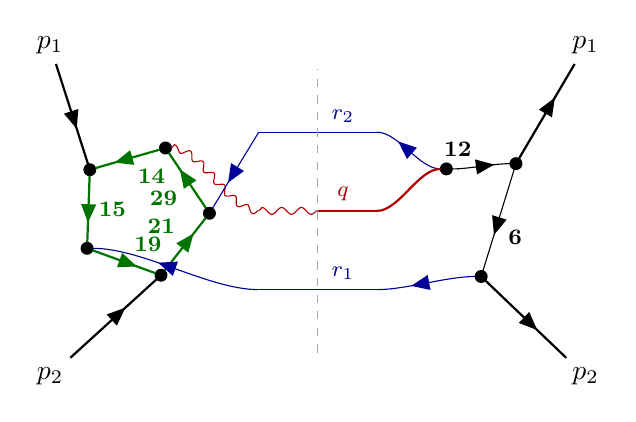
\begin{tikzpicture}
\begin{feynman}
\vertex (Lp1) at (-3.400,2.100) {$p_1$};
\vertex (Lp2) at (-3.400,-2.100) {$p_2$};
\vertex (Lcr1) at (-0.750,-1.000);
\vertex (Lcr2) at (-0.750,1.000);
\vertex (Lcq) at (-0.750,0.000);
\vertex (Mq) at (0,0.000);
\vertex[dot] (Lv0) at (-1.934,0.799) {};
\vertex[dot] (Lv1) at (-2.895,0.523) {};
\vertex[dot] (Lv2) at (-2.930,-0.475) {};
\vertex[dot] (Lv3) at (-1.991,-0.817) {};
\vertex[dot] (Lv4) at (-1.376,-0.030) {};
\vertex (Rp1) at (3.400,2.100) {$p_1$};
\vertex (Rp2) at (3.400,-2.100) {$p_2$};
\vertex (Rcr1) at (0.750,-1.000);
\vertex (Rcr2) at (0.750,1.000);
\vertex (Rcq) at (0.750,0.000);
\vertex[dot] (R6) at (2.075,-0.833) {};
\vertex[dot] (R12) at (2.517,0.600) {};
\vertex[dot] (Rroot) at (1.633,0.533) {};
\diagram* {
(Lv0) -- [plain, thick, green!45!black, with arrow=0.55, edge label={\footnotesize\bfseries 14}] (Lv1),
(Lv1) -- [plain, thick, green!45!black, with arrow=0.55, edge label={\footnotesize\bfseries 15}] (Lv2),
(Lv2) -- [plain, thick, green!45!black, with arrow=0.55, edge label={\footnotesize\bfseries 19}] (Lv3),
(Lv3) -- [plain, thick, green!45!black, with arrow=0.55, edge label={\footnotesize\bfseries 21}] (Lv4),
(Lv4) -- [plain, thick, green!45!black, with arrow=0.55, edge label={\footnotesize\bfseries 29}] (Lv0),
(Lcq) -- [boson, red!70!black, out=180, in=0, looseness=0.75] (Lv0),
(Lp1) -- [plain, thick, with arrow=0.55] (Lv1),
(Lcr1) -- [plain, blue!60!black, out=180, in=0, looseness=0.75, with arrow=0.55] (Lv2),
(Lp2) -- [plain, thick, with arrow=0.55] (Lv3),
(Lcr2) -- [plain, blue!60!black, with arrow=0.55] (Lv4),
(R12) -- [plain, with arrow=0.55, edge label={\footnotesize\bfseries 6}] (R6),
(Rroot) -- [plain, out=0, in=180, looseness=0.75, with arrow=0.55, edge label={\footnotesize\bfseries 12}] (R12),
(R12) -- [plain, thick, with arrow=0.55] (Rp1),
(R6) -- [plain, thick, with arrow=0.55] (Rp2),
(R6) -- [plain, blue!60!black, out=180, in=0, looseness=0.75, with arrow=0.55] (Rcr1),
(Rroot) -- [plain, blue!60!black, out=180, in=0, looseness=0.75, with arrow=0.55] (Rcr2),
(Rroot) -- [plain, red!70!black, double, double distance=1.2pt, thick, out=180, in=0, looseness=0.75] (Rcq),
(Rcr1) -- [plain, blue!60!black] (Lcr1),
(Rcr2) -- [plain, blue!60!black] (Lcr2),
(Rcq) -- [plain, red!70!black, double, double distance=1.2pt, thick] (Mq) -- [boson, red!70!black] (Lcq),
};
\end{feynman}
\draw[dashed, gray!70] (0,-1.80) -- (0,1.80);
\node[font=\footnotesize, blue!60!black, above] at (0.32,-1.00) {$r_1$};
\node[font=\footnotesize, blue!60!black, above] at (0.32,1.00) {$r_2$};
\node[font=\footnotesize, red!70!black, above] at (0.32,0.00) {$q$};
\end{tikzpicture}}\\[2mm]\textbf{topo12} (RR family 21, pentagon q-p1-r1-p2-r2)\\[2pt]{\footnotesize\begin{tabular}{@{}r@{\ \ }l@{\ \ }l@{}}\textbf{14} & $(k_1)^2$ & loop\\
\textbf{15} & $(k_1+p_1)^2$ & loop\\
\textbf{19} & $(k_1+p_1+r_1)^2$ & loop\\
\textbf{21} & $(k_1+p_1+p_2+r_1)^2$ & loop\\
\textbf{29} & $(k_1+p_1+p_2+r_1+r_2)^2$ & loop\\
\textbf{6} & $(p_2+r_1)^2$ & conjugate\\
\textbf{12} & $(p_1+p_2+r_1)^2$ & conjugate\\
\textbf{8} & $(p_2+r_2)^2$ & \textcolor{red}{irreducible numerator}\\\end{tabular}}\end{minipage}

\bigskip

\begin{minipage}[t]{0.48\textwidth}\centering\resizebox{0.9\linewidth}{!}{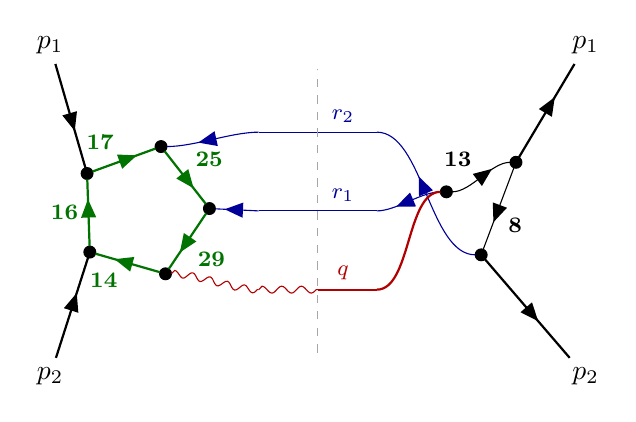
\begin{tikzpicture}
\begin{feynman}
\vertex (Lp1) at (-3.400,2.100) {$p_1$};
\vertex (Lp2) at (-3.400,-2.100) {$p_2$};
\vertex (Lcr1) at (-0.750,0.000);
\vertex (Lcr2) at (-0.750,1.000);
\vertex (Lcq) at (-0.750,-1.000);
\vertex (Mq) at (0,-1.000);
\vertex[dot] (Lv0) at (-1.934,-0.799) {};
\vertex[dot] (Lv1) at (-2.895,-0.523) {};
\vertex[dot] (Lv2) at (-2.930,0.475) {};
\vertex[dot] (Lv3) at (-1.991,0.817) {};
\vertex[dot] (Lv4) at (-1.376,0.030) {};
\vertex (Rp1) at (3.400,2.100) {$p_1$};
\vertex (Rp2) at (3.400,-2.100) {$p_2$};
\vertex (Rcr1) at (0.750,0.000);
\vertex (Rcr2) at (0.750,1.000);
\vertex (Rcq) at (0.750,-1.000);
\vertex[dot] (R8) at (2.075,-0.558) {};
\vertex[dot] (R13) at (2.517,0.617) {};
\vertex[dot] (Rroot) at (1.633,0.242) {};
\diagram* {
(Lv0) -- [plain, thick, green!45!black, with arrow=0.55, edge label={\footnotesize\bfseries 14}] (Lv1),
(Lv1) -- [plain, thick, green!45!black, with arrow=0.55, edge label={\footnotesize\bfseries 16}] (Lv2),
(Lv2) -- [plain, thick, green!45!black, with arrow=0.55, edge label={\footnotesize\bfseries 17}] (Lv3),
(Lv3) -- [plain, thick, green!45!black, with arrow=0.55, edge label={\footnotesize\bfseries 25}] (Lv4),
(Lv4) -- [plain, thick, green!45!black, with arrow=0.55, edge label={\footnotesize\bfseries 29}] (Lv0),
(Lcq) -- [boson, red!70!black, out=180, in=0, looseness=0.75] (Lv0),
(Lp2) -- [plain, thick, with arrow=0.55] (Lv1),
(Lp1) -- [plain, thick, with arrow=0.55] (Lv2),
(Lcr2) -- [plain, blue!60!black, out=180, in=0, looseness=0.75, with arrow=0.55] (Lv3),
(Lcr1) -- [plain, blue!60!black, with arrow=0.55] (Lv4),
(R13) -- [plain, with arrow=0.55, edge label={\footnotesize\bfseries 8}] (R8),
(Rroot) -- [plain, out=0, in=180, looseness=0.75, with arrow=0.55, edge label={\footnotesize\bfseries 13}] (R13),
(R13) -- [plain, thick, with arrow=0.55] (Rp1),
(R8) -- [plain, thick, with arrow=0.55] (Rp2),
(Rroot) -- [plain, blue!60!black, out=180, in=0, looseness=0.75, with arrow=0.55] (Rcr1),
(R8) -- [plain, blue!60!black, out=180, in=0, looseness=0.75, with arrow=0.55] (Rcr2),
(Rroot) -- [plain, red!70!black, double, double distance=1.2pt, thick, out=180, in=0, looseness=0.75] (Rcq),
(Rcr1) -- [plain, blue!60!black] (Lcr1),
(Rcr2) -- [plain, blue!60!black] (Lcr2),
(Rcq) -- [plain, red!70!black, double, double distance=1.2pt, thick] (Mq) -- [boson, red!70!black] (Lcq),
};
\end{feynman}
\draw[dashed, gray!70] (0,-1.80) -- (0,1.80);
\node[font=\footnotesize, blue!60!black, above] at (0.32,0.00) {$r_1$};
\node[font=\footnotesize, blue!60!black, above] at (0.32,1.00) {$r_2$};
\node[font=\footnotesize, red!70!black, above] at (0.32,-1.00) {$q$};
\end{tikzpicture}}\\[2mm]\textbf{topo13} (RR family 31, pentagon q-p2-p1-r2-r1)\\[2pt]{\footnotesize\begin{tabular}{@{}r@{\ \ }l@{\ \ }l@{}}\textbf{14} & $(k_1)^2$ & loop\\
\textbf{16} & $(k_1+p_2)^2$ & loop\\
\textbf{17} & $(k_1+p_1+p_2)^2$ & loop\\
\textbf{25} & $(k_1+p_1+p_2+r_2)^2$ & loop\\
\textbf{29} & $(k_1+p_1+p_2+r_1+r_2)^2$ & loop\\
\textbf{8} & $(p_2+r_2)^2$ & conjugate\\
\textbf{13} & $(p_1+p_2+r_2)^2$ & conjugate\\
\textbf{11} & $(r_1+r_2)^2$ & \textcolor{red}{irreducible numerator}\\\end{tabular}}\end{minipage}\hfill%
\begin{minipage}[t]{0.48\textwidth}\centering\resizebox{0.9\linewidth}{!}{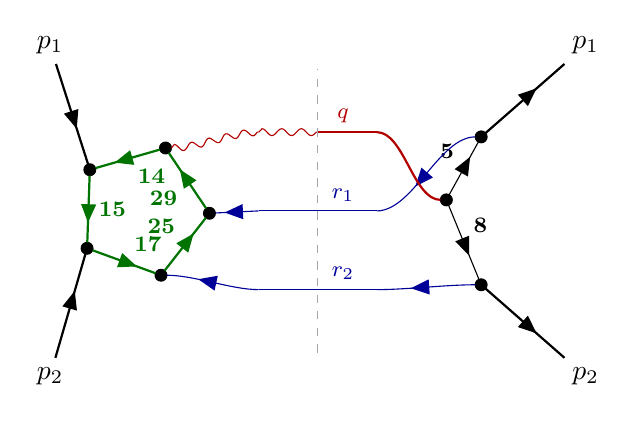
\begin{tikzpicture}
\begin{feynman}
\vertex (Lp1) at (-3.400,2.100) {$p_1$};
\vertex (Lp2) at (-3.400,-2.100) {$p_2$};
\vertex (Lcr1) at (-0.750,0.000);
\vertex (Lcr2) at (-0.750,-1.000);
\vertex (Lcq) at (-0.750,1.000);
\vertex (Mq) at (0,1.000);
\vertex[dot] (Lv0) at (-1.934,0.799) {};
\vertex[dot] (Lv1) at (-2.895,0.523) {};
\vertex[dot] (Lv2) at (-2.930,-0.475) {};
\vertex[dot] (Lv3) at (-1.991,-0.817) {};
\vertex[dot] (Lv4) at (-1.376,-0.030) {};
\vertex (Rp1) at (3.400,2.100) {$p_1$};
\vertex (Rp2) at (3.400,-2.100) {$p_2$};
\vertex (Rcr1) at (0.750,0.000);
\vertex (Rcr2) at (0.750,-1.000);
\vertex (Rcq) at (0.750,1.000);
\vertex[dot] (R5) at (2.075,0.940) {};
\vertex[dot] (Rroot) at (1.633,0.140) {};
\vertex[dot] (R8) at (2.075,-0.938) {};
\diagram* {
(Lv0) -- [plain, thick, green!45!black, with arrow=0.55, edge label={\footnotesize\bfseries 14}] (Lv1),
(Lv1) -- [plain, thick, green!45!black, with arrow=0.55, edge label={\footnotesize\bfseries 15}] (Lv2),
(Lv2) -- [plain, thick, green!45!black, with arrow=0.55, edge label={\footnotesize\bfseries 17}] (Lv3),
(Lv3) -- [plain, thick, green!45!black, with arrow=0.55, edge label={\footnotesize\bfseries 25}] (Lv4),
(Lv4) -- [plain, thick, green!45!black, with arrow=0.55, edge label={\footnotesize\bfseries 29}] (Lv0),
(Lcq) -- [boson, red!70!black, out=180, in=0, looseness=0.75] (Lv0),
(Lp1) -- [plain, thick, with arrow=0.55] (Lv1),
(Lp2) -- [plain, thick, with arrow=0.55] (Lv2),
(Lcr2) -- [plain, blue!60!black, out=180, in=0, looseness=0.75, with arrow=0.55] (Lv3),
(Lcr1) -- [plain, blue!60!black, with arrow=0.55] (Lv4),
(Rroot) -- [plain, with arrow=0.55, edge label={\footnotesize\bfseries 5}] (R5),
(Rroot) -- [plain, with arrow=0.55, edge label={\footnotesize\bfseries 8}] (R8),
(R5) -- [plain, thick, with arrow=0.55] (Rp1),
(R8) -- [plain, thick, with arrow=0.55] (Rp2),
(R5) -- [plain, blue!60!black, out=180, in=0, looseness=0.75, with arrow=0.55] (Rcr1),
(R8) -- [plain, blue!60!black, out=180, in=0, looseness=0.75, with arrow=0.55] (Rcr2),
(Rroot) -- [plain, red!70!black, double, double distance=1.2pt, thick, out=180, in=0, looseness=0.75] (Rcq),
(Rcr1) -- [plain, blue!60!black] (Lcr1),
(Rcr2) -- [plain, blue!60!black] (Lcr2),
(Rcq) -- [plain, red!70!black, double, double distance=1.2pt, thick] (Mq) -- [boson, red!70!black] (Lcq),
};
\end{feynman}
\draw[dashed, gray!70] (0,-1.80) -- (0,1.80);
\node[font=\footnotesize, blue!60!black, above] at (0.32,0.00) {$r_1$};
\node[font=\footnotesize, blue!60!black, above] at (0.32,-1.00) {$r_2$};
\node[font=\footnotesize, red!70!black, above] at (0.32,1.00) {$q$};
\end{tikzpicture}}\\[2mm]\textbf{topo14} (RR family 6, pentagon q-p1-p2-r2-r1)\\[2pt]{\footnotesize\begin{tabular}{@{}r@{\ \ }l@{\ \ }l@{}}\textbf{14} & $(k_1)^2$ & loop\\
\textbf{15} & $(k_1+p_1)^2$ & loop\\
\textbf{17} & $(k_1+p_1+p_2)^2$ & loop\\
\textbf{25} & $(k_1+p_1+p_2+r_2)^2$ & loop\\
\textbf{29} & $(k_1+p_1+p_2+r_1+r_2)^2$ & loop\\
\textbf{5} & $(p_1+r_1)^2$ & conjugate\\
\textbf{8} & $(p_2+r_2)^2$ & conjugate\\
\textbf{9} & $(p_1+r_1+r_2)^2$ & \textcolor{red}{irreducible numerator}\\\end{tabular}}\end{minipage}

\bigskip

\begin{minipage}[t]{0.48\textwidth}\centering\resizebox{0.9\linewidth}{!}{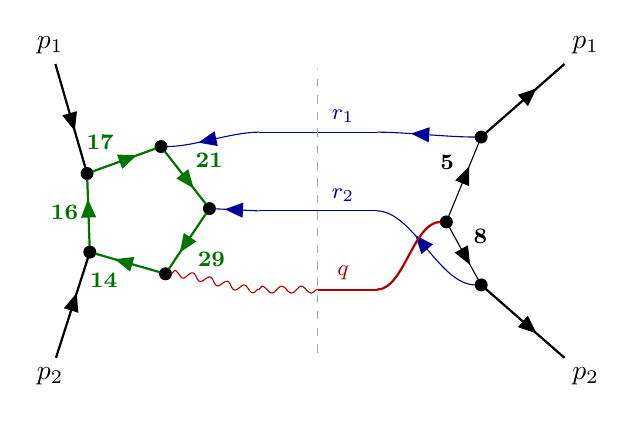
\begin{tikzpicture}
\begin{feynman}
\vertex (Lp1) at (-3.400,2.100) {$p_1$};
\vertex (Lp2) at (-3.400,-2.100) {$p_2$};
\vertex (Lcr1) at (-0.750,1.000);
\vertex (Lcr2) at (-0.750,0.000);
\vertex (Lcq) at (-0.750,-1.000);
\vertex (Mq) at (0,-1.000);
\vertex[dot] (Lv0) at (-1.934,-0.799) {};
\vertex[dot] (Lv1) at (-2.895,-0.523) {};
\vertex[dot] (Lv2) at (-2.930,0.475) {};
\vertex[dot] (Lv3) at (-1.991,0.817) {};
\vertex[dot] (Lv4) at (-1.376,0.030) {};
\vertex (Rp1) at (3.400,2.100) {$p_1$};
\vertex (Rp2) at (3.400,-2.100) {$p_2$};
\vertex (Rcr1) at (0.750,1.000);
\vertex (Rcr2) at (0.750,0.000);
\vertex (Rcq) at (0.750,-1.000);
\vertex[dot] (R5) at (2.075,0.938) {};
\vertex[dot] (Rroot) at (1.633,-0.140) {};
\vertex[dot] (R8) at (2.075,-0.940) {};
\diagram* {
(Lv0) -- [plain, thick, green!45!black, with arrow=0.55, edge label={\footnotesize\bfseries 14}] (Lv1),
(Lv1) -- [plain, thick, green!45!black, with arrow=0.55, edge label={\footnotesize\bfseries 16}] (Lv2),
(Lv2) -- [plain, thick, green!45!black, with arrow=0.55, edge label={\footnotesize\bfseries 17}] (Lv3),
(Lv3) -- [plain, thick, green!45!black, with arrow=0.55, edge label={\footnotesize\bfseries 21}] (Lv4),
(Lv4) -- [plain, thick, green!45!black, with arrow=0.55, edge label={\footnotesize\bfseries 29}] (Lv0),
(Lcq) -- [boson, red!70!black, out=180, in=0, looseness=0.75] (Lv0),
(Lp2) -- [plain, thick, with arrow=0.55] (Lv1),
(Lp1) -- [plain, thick, with arrow=0.55] (Lv2),
(Lcr1) -- [plain, blue!60!black, out=180, in=0, looseness=0.75, with arrow=0.55] (Lv3),
(Lcr2) -- [plain, blue!60!black, with arrow=0.55] (Lv4),
(Rroot) -- [plain, with arrow=0.55, edge label={\footnotesize\bfseries 5}] (R5),
(Rroot) -- [plain, with arrow=0.55, edge label={\footnotesize\bfseries 8}] (R8),
(R5) -- [plain, thick, with arrow=0.55] (Rp1),
(R8) -- [plain, thick, with arrow=0.55] (Rp2),
(R5) -- [plain, blue!60!black, out=180, in=0, looseness=0.75, with arrow=0.55] (Rcr1),
(R8) -- [plain, blue!60!black, out=180, in=0, looseness=0.75, with arrow=0.55] (Rcr2),
(Rroot) -- [plain, red!70!black, double, double distance=1.2pt, thick, out=180, in=0, looseness=0.75] (Rcq),
(Rcr1) -- [plain, blue!60!black] (Lcr1),
(Rcr2) -- [plain, blue!60!black] (Lcr2),
(Rcq) -- [plain, red!70!black, double, double distance=1.2pt, thick] (Mq) -- [boson, red!70!black] (Lcq),
};
\end{feynman}
\draw[dashed, gray!70] (0,-1.80) -- (0,1.80);
\node[font=\footnotesize, blue!60!black, above] at (0.32,1.00) {$r_1$};
\node[font=\footnotesize, blue!60!black, above] at (0.32,0.00) {$r_2$};
\node[font=\footnotesize, red!70!black, above] at (0.32,-1.00) {$q$};
\end{tikzpicture}}\\[2mm]\textbf{topo15} (RR family 18, pentagon q-p2-p1-r1-r2)\\[2pt]{\footnotesize\begin{tabular}{@{}r@{\ \ }l@{\ \ }l@{}}\textbf{14} & $(k_1)^2$ & loop\\
\textbf{16} & $(k_1+p_2)^2$ & loop\\
\textbf{17} & $(k_1+p_1+p_2)^2$ & loop\\
\textbf{21} & $(k_1+p_1+p_2+r_1)^2$ & loop\\
\textbf{29} & $(k_1+p_1+p_2+r_1+r_2)^2$ & loop\\
\textbf{5} & $(p_1+r_1)^2$ & conjugate\\
\textbf{8} & $(p_2+r_2)^2$ & conjugate\\
\textbf{13} & $(p_1+p_2+r_2)^2$ & \textcolor{red}{irreducible numerator}\\\end{tabular}}\end{minipage}\hfill%
\begin{minipage}[t]{0.48\textwidth}\centering\resizebox{0.9\linewidth}{!}{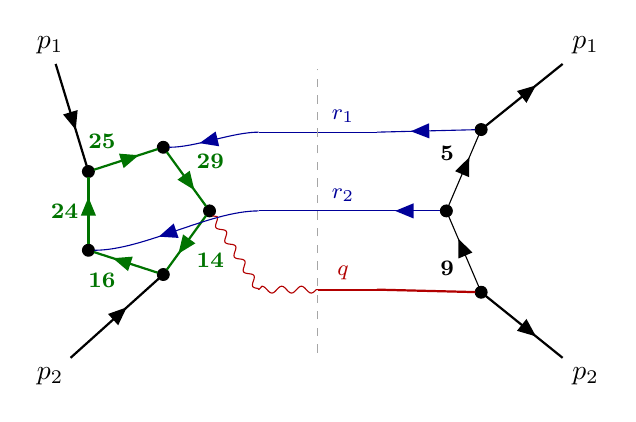
\begin{tikzpicture}
\begin{feynman}
\vertex (Lp1) at (-3.400,2.100) {$p_1$};
\vertex (Lp2) at (-3.400,-2.100) {$p_2$};
\vertex (Lcr1) at (-0.750,1.000);
\vertex (Lcr2) at (-0.750,0.000);
\vertex (Lcq) at (-0.750,-1.000);
\vertex (Mq) at (0,-1.000);
\vertex[dot] (Lv0) at (-1.375,0.000) {};
\vertex[dot] (Lv1) at (-1.962,-0.808) {};
\vertex[dot] (Lv2) at (-2.913,-0.500) {};
\vertex[dot] (Lv3) at (-2.913,0.500) {};
\vertex[dot] (Lv4) at (-1.962,0.808) {};
\vertex (Rp1) at (3.400,2.100) {$p_1$};
\vertex (Rp2) at (3.400,-2.100) {$p_2$};
\vertex (Rcr1) at (0.750,1.000);
\vertex (Rcr2) at (0.750,0.000);
\vertex (Rcq) at (0.750,-1.000);
\vertex[dot] (R5) at (2.075,1.033) {};
\vertex[dot] (R9) at (1.633,0.000) {};
\vertex[dot] (Rroot) at (2.075,-1.033) {};
\diagram* {
(Lv0) -- [plain, thick, green!45!black, with arrow=0.55, edge label={\footnotesize\bfseries 14}] (Lv1),
(Lv1) -- [plain, thick, green!45!black, with arrow=0.55, edge label={\footnotesize\bfseries 16}] (Lv2),
(Lv2) -- [plain, thick, green!45!black, with arrow=0.55, edge label={\footnotesize\bfseries 24}] (Lv3),
(Lv3) -- [plain, thick, green!45!black, with arrow=0.55, edge label={\footnotesize\bfseries 25}] (Lv4),
(Lv4) -- [plain, thick, green!45!black, with arrow=0.55, edge label={\footnotesize\bfseries 29}] (Lv0),
(Lcq) -- [boson, red!70!black] (Lv0),
(Lp2) -- [plain, thick, with arrow=0.55] (Lv1),
(Lcr2) -- [plain, blue!60!black, out=180, in=0, looseness=0.75, with arrow=0.55] (Lv2),
(Lp1) -- [plain, thick, with arrow=0.55] (Lv3),
(Lcr1) -- [plain, blue!60!black, out=180, in=0, looseness=0.75, with arrow=0.55] (Lv4),
(R9) -- [plain, with arrow=0.55, edge label={\footnotesize\bfseries 5}] (R5),
(Rroot) -- [plain, with arrow=0.55, edge label={\footnotesize\bfseries 9}] (R9),
(R5) -- [plain, thick, with arrow=0.55] (Rp1),
(Rroot) -- [plain, thick, with arrow=0.55] (Rp2),
(R5) -- [plain, blue!60!black, with arrow=0.55] (Rcr1),
(R9) -- [plain, blue!60!black, with arrow=0.55] (Rcr2),
(Rroot) -- [plain, red!70!black, double, double distance=1.2pt, thick] (Rcq),
(Rcr1) -- [plain, blue!60!black] (Lcr1),
(Rcr2) -- [plain, blue!60!black] (Lcr2),
(Rcq) -- [plain, red!70!black, double, double distance=1.2pt, thick] (Mq) -- [boson, red!70!black] (Lcq),
};
\end{feynman}
\draw[dashed, gray!70] (0,-1.80) -- (0,1.80);
\node[font=\footnotesize, blue!60!black, above] at (0.32,1.00) {$r_1$};
\node[font=\footnotesize, blue!60!black, above] at (0.32,0.00) {$r_2$};
\node[font=\footnotesize, red!70!black, above] at (0.32,-1.00) {$q$};
\end{tikzpicture}}\\[2mm]\textbf{topo16} (RR family 32, pentagon q-p2-r2-p1-r1)\\[2pt]{\footnotesize\begin{tabular}{@{}r@{\ \ }l@{\ \ }l@{}}\textbf{14} & $(k_1)^2$ & loop\\
\textbf{16} & $(k_1+p_2)^2$ & loop\\
\textbf{24} & $(k_1+p_2+r_2)^2$ & loop\\
\textbf{25} & $(k_1+p_1+p_2+r_2)^2$ & loop\\
\textbf{29} & $(k_1+p_1+p_2+r_1+r_2)^2$ & loop\\
\textbf{5} & $(p_1+r_1)^2$ & conjugate\\
\textbf{9} & $(p_1+r_1+r_2)^2$ & conjugate\\
\textbf{13} & $(p_1+p_2+r_2)^2$ & \textcolor{red}{irreducible numerator}\\\end{tabular}}\end{minipage}

\bigskip

\begin{minipage}[t]{0.48\textwidth}\centering\resizebox{0.9\linewidth}{!}{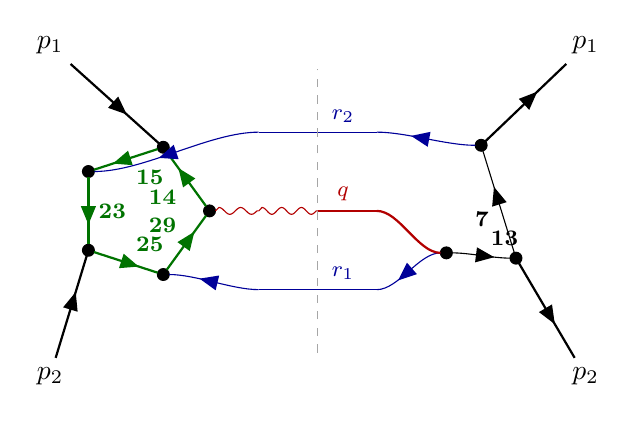
\begin{tikzpicture}
\begin{feynman}
\vertex (Lp1) at (-3.400,2.100) {$p_1$};
\vertex (Lp2) at (-3.400,-2.100) {$p_2$};
\vertex (Lcr1) at (-0.750,-1.000);
\vertex (Lcr2) at (-0.750,1.000);
\vertex (Lcq) at (-0.750,0.000);
\vertex (Mq) at (0,0.000);
\vertex[dot] (Lv0) at (-1.375,0.000) {};
\vertex[dot] (Lv1) at (-1.962,0.808) {};
\vertex[dot] (Lv2) at (-2.913,0.500) {};
\vertex[dot] (Lv3) at (-2.913,-0.500) {};
\vertex[dot] (Lv4) at (-1.962,-0.808) {};
\vertex (Rp1) at (3.400,2.100) {$p_1$};
\vertex (Rp2) at (3.400,-2.100) {$p_2$};
\vertex (Rcr1) at (0.750,-1.000);
\vertex (Rcr2) at (0.750,1.000);
\vertex (Rcq) at (0.750,0.000);
\vertex[dot] (R7) at (2.075,0.833) {};
\vertex[dot] (R13) at (2.517,-0.600) {};
\vertex[dot] (Rroot) at (1.633,-0.533) {};
\diagram* {
(Lv0) -- [plain, thick, green!45!black, with arrow=0.55, edge label={\footnotesize\bfseries 14}] (Lv1),
(Lv1) -- [plain, thick, green!45!black, with arrow=0.55, edge label={\footnotesize\bfseries 15}] (Lv2),
(Lv2) -- [plain, thick, green!45!black, with arrow=0.55, edge label={\footnotesize\bfseries 23}] (Lv3),
(Lv3) -- [plain, thick, green!45!black, with arrow=0.55, edge label={\footnotesize\bfseries 25}] (Lv4),
(Lv4) -- [plain, thick, green!45!black, with arrow=0.55, edge label={\footnotesize\bfseries 29}] (Lv0),
(Lcq) -- [boson, red!70!black] (Lv0),
(Lp1) -- [plain, thick, with arrow=0.55] (Lv1),
(Lcr2) -- [plain, blue!60!black, out=180, in=0, looseness=0.75, with arrow=0.55] (Lv2),
(Lp2) -- [plain, thick, with arrow=0.55] (Lv3),
(Lcr1) -- [plain, blue!60!black, out=180, in=0, looseness=0.75, with arrow=0.55] (Lv4),
(R13) -- [plain, with arrow=0.55, edge label={\footnotesize\bfseries 7}] (R7),
(Rroot) -- [plain, out=0, in=180, looseness=0.75, with arrow=0.55, edge label={\footnotesize\bfseries 13}] (R13),
(R7) -- [plain, thick, with arrow=0.55] (Rp1),
(R13) -- [plain, thick, with arrow=0.55] (Rp2),
(Rroot) -- [plain, blue!60!black, out=180, in=0, looseness=0.75, with arrow=0.55] (Rcr1),
(R7) -- [plain, blue!60!black, out=180, in=0, looseness=0.75, with arrow=0.55] (Rcr2),
(Rroot) -- [plain, red!70!black, double, double distance=1.2pt, thick, out=180, in=0, looseness=0.75] (Rcq),
(Rcr1) -- [plain, blue!60!black] (Lcr1),
(Rcr2) -- [plain, blue!60!black] (Lcr2),
(Rcq) -- [plain, red!70!black, double, double distance=1.2pt, thick] (Mq) -- [boson, red!70!black] (Lcq),
};
\end{feynman}
\draw[dashed, gray!70] (0,-1.80) -- (0,1.80);
\node[font=\footnotesize, blue!60!black, above] at (0.32,-1.00) {$r_1$};
\node[font=\footnotesize, blue!60!black, above] at (0.32,1.00) {$r_2$};
\node[font=\footnotesize, red!70!black, above] at (0.32,0.00) {$q$};
\end{tikzpicture}}\\[2mm]\textbf{topo17} (RR family 28, pentagon q-p1-r2-p2-r1)\\[2pt]{\footnotesize\begin{tabular}{@{}r@{\ \ }l@{\ \ }l@{}}\textbf{14} & $(k_1)^2$ & loop\\
\textbf{15} & $(k_1+p_1)^2$ & loop\\
\textbf{23} & $(k_1+p_1+r_2)^2$ & loop\\
\textbf{25} & $(k_1+p_1+p_2+r_2)^2$ & loop\\
\textbf{29} & $(k_1+p_1+p_2+r_1+r_2)^2$ & loop\\
\textbf{7} & $(p_1+r_2)^2$ & conjugate\\
\textbf{13} & $(p_1+p_2+r_2)^2$ & conjugate\\
\textbf{10} & $(p_2+r_1+r_2)^2$ & \textcolor{red}{irreducible numerator}\\\end{tabular}}\end{minipage}\hfill%
\begin{minipage}[t]{0.48\textwidth}\centering\resizebox{0.9\linewidth}{!}{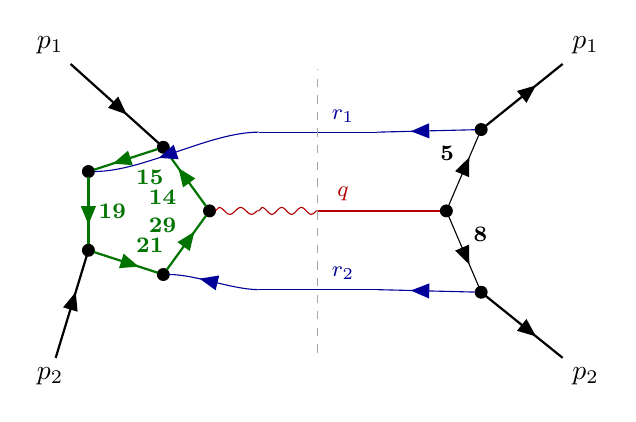
\begin{tikzpicture}
\begin{feynman}
\vertex (Lp1) at (-3.400,2.100) {$p_1$};
\vertex (Lp2) at (-3.400,-2.100) {$p_2$};
\vertex (Lcr1) at (-0.750,1.000);
\vertex (Lcr2) at (-0.750,-1.000);
\vertex (Lcq) at (-0.750,0.000);
\vertex (Mq) at (0,0.000);
\vertex[dot] (Lv0) at (-1.375,0.000) {};
\vertex[dot] (Lv1) at (-1.962,0.808) {};
\vertex[dot] (Lv2) at (-2.913,0.500) {};
\vertex[dot] (Lv3) at (-2.913,-0.500) {};
\vertex[dot] (Lv4) at (-1.962,-0.808) {};
\vertex (Rp1) at (3.400,2.100) {$p_1$};
\vertex (Rp2) at (3.400,-2.100) {$p_2$};
\vertex (Rcr1) at (0.750,1.000);
\vertex (Rcr2) at (0.750,-1.000);
\vertex (Rcq) at (0.750,0.000);
\vertex[dot] (R5) at (2.075,1.033) {};
\vertex[dot] (Rroot) at (1.633,0.000) {};
\vertex[dot] (R8) at (2.075,-1.033) {};
\diagram* {
(Lv0) -- [plain, thick, green!45!black, with arrow=0.55, edge label={\footnotesize\bfseries 14}] (Lv1),
(Lv1) -- [plain, thick, green!45!black, with arrow=0.55, edge label={\footnotesize\bfseries 15}] (Lv2),
(Lv2) -- [plain, thick, green!45!black, with arrow=0.55, edge label={\footnotesize\bfseries 19}] (Lv3),
(Lv3) -- [plain, thick, green!45!black, with arrow=0.55, edge label={\footnotesize\bfseries 21}] (Lv4),
(Lv4) -- [plain, thick, green!45!black, with arrow=0.55, edge label={\footnotesize\bfseries 29}] (Lv0),
(Lcq) -- [boson, red!70!black] (Lv0),
(Lp1) -- [plain, thick, with arrow=0.55] (Lv1),
(Lcr1) -- [plain, blue!60!black, out=180, in=0, looseness=0.75, with arrow=0.55] (Lv2),
(Lp2) -- [plain, thick, with arrow=0.55] (Lv3),
(Lcr2) -- [plain, blue!60!black, out=180, in=0, looseness=0.75, with arrow=0.55] (Lv4),
(Rroot) -- [plain, with arrow=0.55, edge label={\footnotesize\bfseries 5}] (R5),
(Rroot) -- [plain, with arrow=0.55, edge label={\footnotesize\bfseries 8}] (R8),
(R5) -- [plain, thick, with arrow=0.55] (Rp1),
(R8) -- [plain, thick, with arrow=0.55] (Rp2),
(R5) -- [plain, blue!60!black, with arrow=0.55] (Rcr1),
(R8) -- [plain, blue!60!black, with arrow=0.55] (Rcr2),
(Rroot) -- [plain, red!70!black, double, double distance=1.2pt, thick] (Rcq),
(Rcr1) -- [plain, blue!60!black] (Lcr1),
(Rcr2) -- [plain, blue!60!black] (Lcr2),
(Rcq) -- [plain, red!70!black, double, double distance=1.2pt, thick] (Mq) -- [boson, red!70!black] (Lcq),
};
\end{feynman}
\draw[dashed, gray!70] (0,-1.80) -- (0,1.80);
\node[font=\footnotesize, blue!60!black, above] at (0.32,1.00) {$r_1$};
\node[font=\footnotesize, blue!60!black, above] at (0.32,-1.00) {$r_2$};
\node[font=\footnotesize, red!70!black, above] at (0.32,0.00) {$q$};
\end{tikzpicture}}\\[2mm]\textbf{topo18} (RR family 2, pentagon q-p1-r1-p2-r2)\\[2pt]{\footnotesize\begin{tabular}{@{}r@{\ \ }l@{\ \ }l@{}}\textbf{14} & $(k_1)^2$ & loop\\
\textbf{15} & $(k_1+p_1)^2$ & loop\\
\textbf{19} & $(k_1+p_1+r_1)^2$ & loop\\
\textbf{21} & $(k_1+p_1+p_2+r_1)^2$ & loop\\
\textbf{29} & $(k_1+p_1+p_2+r_1+r_2)^2$ & loop\\
\textbf{5} & $(p_1+r_1)^2$ & conjugate\\
\textbf{8} & $(p_2+r_2)^2$ & conjugate\\
\textbf{6} & $(p_2+r_1)^2$ & \textcolor{red}{irreducible numerator}\\\end{tabular}}\end{minipage}

\bigskip

\begin{minipage}[t]{0.48\textwidth}\centering\resizebox{0.9\linewidth}{!}{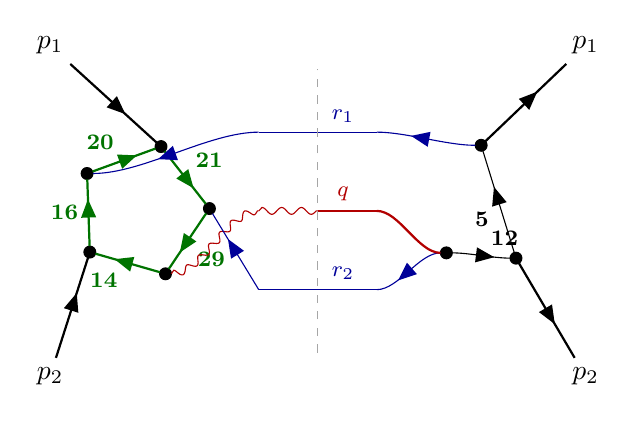
\begin{tikzpicture}
\begin{feynman}
\vertex (Lp1) at (-3.400,2.100) {$p_1$};
\vertex (Lp2) at (-3.400,-2.100) {$p_2$};
\vertex (Lcr1) at (-0.750,1.000);
\vertex (Lcr2) at (-0.750,-1.000);
\vertex (Lcq) at (-0.750,0.000);
\vertex (Mq) at (0,0.000);
\vertex[dot] (Lv0) at (-1.934,-0.799) {};
\vertex[dot] (Lv1) at (-2.895,-0.523) {};
\vertex[dot] (Lv2) at (-2.930,0.475) {};
\vertex[dot] (Lv3) at (-1.991,0.817) {};
\vertex[dot] (Lv4) at (-1.376,0.030) {};
\vertex (Rp1) at (3.400,2.100) {$p_1$};
\vertex (Rp2) at (3.400,-2.100) {$p_2$};
\vertex (Rcr1) at (0.750,1.000);
\vertex (Rcr2) at (0.750,-1.000);
\vertex (Rcq) at (0.750,0.000);
\vertex[dot] (R5) at (2.075,0.833) {};
\vertex[dot] (R12) at (2.517,-0.600) {};
\vertex[dot] (Rroot) at (1.633,-0.533) {};
\diagram* {
(Lv0) -- [plain, thick, green!45!black, with arrow=0.55, edge label={\footnotesize\bfseries 14}] (Lv1),
(Lv1) -- [plain, thick, green!45!black, with arrow=0.55, edge label={\footnotesize\bfseries 16}] (Lv2),
(Lv2) -- [plain, thick, green!45!black, with arrow=0.55, edge label={\footnotesize\bfseries 20}] (Lv3),
(Lv3) -- [plain, thick, green!45!black, with arrow=0.55, edge label={\footnotesize\bfseries 21}] (Lv4),
(Lv4) -- [plain, thick, green!45!black, with arrow=0.55, edge label={\footnotesize\bfseries 29}] (Lv0),
(Lcq) -- [boson, red!70!black, out=180, in=0, looseness=0.75] (Lv0),
(Lp2) -- [plain, thick, with arrow=0.55] (Lv1),
(Lcr1) -- [plain, blue!60!black, out=180, in=0, looseness=0.75, with arrow=0.55] (Lv2),
(Lp1) -- [plain, thick, with arrow=0.55] (Lv3),
(Lcr2) -- [plain, blue!60!black, with arrow=0.55] (Lv4),
(R12) -- [plain, with arrow=0.55, edge label={\footnotesize\bfseries 5}] (R5),
(Rroot) -- [plain, out=0, in=180, looseness=0.75, with arrow=0.55, edge label={\footnotesize\bfseries 12}] (R12),
(R5) -- [plain, thick, with arrow=0.55] (Rp1),
(R12) -- [plain, thick, with arrow=0.55] (Rp2),
(R5) -- [plain, blue!60!black, out=180, in=0, looseness=0.75, with arrow=0.55] (Rcr1),
(Rroot) -- [plain, blue!60!black, out=180, in=0, looseness=0.75, with arrow=0.55] (Rcr2),
(Rroot) -- [plain, red!70!black, double, double distance=1.2pt, thick, out=180, in=0, looseness=0.75] (Rcq),
(Rcr1) -- [plain, blue!60!black] (Lcr1),
(Rcr2) -- [plain, blue!60!black] (Lcr2),
(Rcq) -- [plain, red!70!black, double, double distance=1.2pt, thick] (Mq) -- [boson, red!70!black] (Lcq),
};
\end{feynman}
\draw[dashed, gray!70] (0,-1.80) -- (0,1.80);
\node[font=\footnotesize, blue!60!black, above] at (0.32,1.00) {$r_1$};
\node[font=\footnotesize, blue!60!black, above] at (0.32,-1.00) {$r_2$};
\node[font=\footnotesize, red!70!black, above] at (0.32,0.00) {$q$};
\end{tikzpicture}}\\[2mm]\textbf{topo19} (RR family 15, pentagon q-p2-r1-p1-r2)\\[2pt]{\footnotesize\begin{tabular}{@{}r@{\ \ }l@{\ \ }l@{}}\textbf{14} & $(k_1)^2$ & loop\\
\textbf{16} & $(k_1+p_2)^2$ & loop\\
\textbf{20} & $(k_1+p_2+r_1)^2$ & loop\\
\textbf{21} & $(k_1+p_1+p_2+r_1)^2$ & loop\\
\textbf{29} & $(k_1+p_1+p_2+r_1+r_2)^2$ & loop\\
\textbf{5} & $(p_1+r_1)^2$ & conjugate\\
\textbf{12} & $(p_1+p_2+r_1)^2$ & conjugate\\
\textbf{7} & $(p_1+r_2)^2$ & \textcolor{red}{irreducible numerator}\\\end{tabular}}\end{minipage}\hfill%
\begin{minipage}[t]{0.48\textwidth}\centering\resizebox{0.9\linewidth}{!}{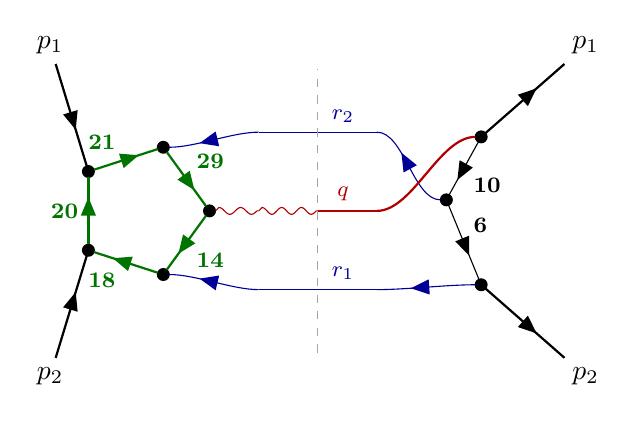
\begin{tikzpicture}
\begin{feynman}
\vertex (Lp1) at (-3.400,2.100) {$p_1$};
\vertex (Lp2) at (-3.400,-2.100) {$p_2$};
\vertex (Lcr1) at (-0.750,-1.000);
\vertex (Lcr2) at (-0.750,1.000);
\vertex (Lcq) at (-0.750,0.000);
\vertex (Mq) at (0,0.000);
\vertex[dot] (Lv0) at (-1.375,0.000) {};
\vertex[dot] (Lv1) at (-1.962,-0.808) {};
\vertex[dot] (Lv2) at (-2.913,-0.500) {};
\vertex[dot] (Lv3) at (-2.913,0.500) {};
\vertex[dot] (Lv4) at (-1.962,0.808) {};
\vertex (Rp1) at (3.400,2.100) {$p_1$};
\vertex (Rp2) at (3.400,-2.100) {$p_2$};
\vertex (Rcr1) at (0.750,-1.000);
\vertex (Rcr2) at (0.750,1.000);
\vertex (Rcq) at (0.750,0.000);
\vertex[dot] (R6) at (2.075,-0.938) {};
\vertex[dot] (R10) at (1.633,0.140) {};
\vertex[dot] (Rroot) at (2.075,0.940) {};
\diagram* {
(Lv0) -- [plain, thick, green!45!black, with arrow=0.55, edge label={\footnotesize\bfseries 14}] (Lv1),
(Lv1) -- [plain, thick, green!45!black, with arrow=0.55, edge label={\footnotesize\bfseries 18}] (Lv2),
(Lv2) -- [plain, thick, green!45!black, with arrow=0.55, edge label={\footnotesize\bfseries 20}] (Lv3),
(Lv3) -- [plain, thick, green!45!black, with arrow=0.55, edge label={\footnotesize\bfseries 21}] (Lv4),
(Lv4) -- [plain, thick, green!45!black, with arrow=0.55, edge label={\footnotesize\bfseries 29}] (Lv0),
(Lcq) -- [boson, red!70!black] (Lv0),
(Lcr1) -- [plain, blue!60!black, out=180, in=0, looseness=0.75, with arrow=0.55] (Lv1),
(Lp2) -- [plain, thick, with arrow=0.55] (Lv2),
(Lp1) -- [plain, thick, with arrow=0.55] (Lv3),
(Lcr2) -- [plain, blue!60!black, out=180, in=0, looseness=0.75, with arrow=0.55] (Lv4),
(R10) -- [plain, with arrow=0.55, edge label={\footnotesize\bfseries 6}] (R6),
(Rroot) -- [plain, with arrow=0.55, edge label={\footnotesize\bfseries 10}] (R10),
(Rroot) -- [plain, thick, with arrow=0.55] (Rp1),
(R6) -- [plain, thick, with arrow=0.55] (Rp2),
(R6) -- [plain, blue!60!black, out=180, in=0, looseness=0.75, with arrow=0.55] (Rcr1),
(R10) -- [plain, blue!60!black, out=180, in=0, looseness=0.75, with arrow=0.55] (Rcr2),
(Rroot) -- [plain, red!70!black, double, double distance=1.2pt, thick, out=180, in=0, looseness=0.75] (Rcq),
(Rcr1) -- [plain, blue!60!black] (Lcr1),
(Rcr2) -- [plain, blue!60!black] (Lcr2),
(Rcq) -- [plain, red!70!black, double, double distance=1.2pt, thick] (Mq) -- [boson, red!70!black] (Lcq),
};
\end{feynman}
\draw[dashed, gray!70] (0,-1.80) -- (0,1.80);
\node[font=\footnotesize, blue!60!black, above] at (0.32,-1.00) {$r_1$};
\node[font=\footnotesize, blue!60!black, above] at (0.32,1.00) {$r_2$};
\node[font=\footnotesize, red!70!black, above] at (0.32,0.00) {$q$};
\end{tikzpicture}}\\[2mm]\textbf{topo20} (RR family 27, pentagon q-r1-p2-p1-r2)\\[2pt]{\footnotesize\begin{tabular}{@{}r@{\ \ }l@{\ \ }l@{}}\textbf{14} & $(k_1)^2$ & loop\\
\textbf{18} & $(k_1+r_1)^2$ & loop\\
\textbf{20} & $(k_1+p_2+r_1)^2$ & loop\\
\textbf{21} & $(k_1+p_1+p_2+r_1)^2$ & loop\\
\textbf{29} & $(k_1+p_1+p_2+r_1+r_2)^2$ & loop\\
\textbf{6} & $(p_2+r_1)^2$ & conjugate\\
\textbf{10} & $(p_2+r_1+r_2)^2$ & conjugate\\
\textbf{13} & $(p_1+p_2+r_2)^2$ & \textcolor{red}{irreducible numerator}\\\end{tabular}}\end{minipage}

\bigskip

\begin{minipage}[t]{0.48\textwidth}\centering\resizebox{0.9\linewidth}{!}{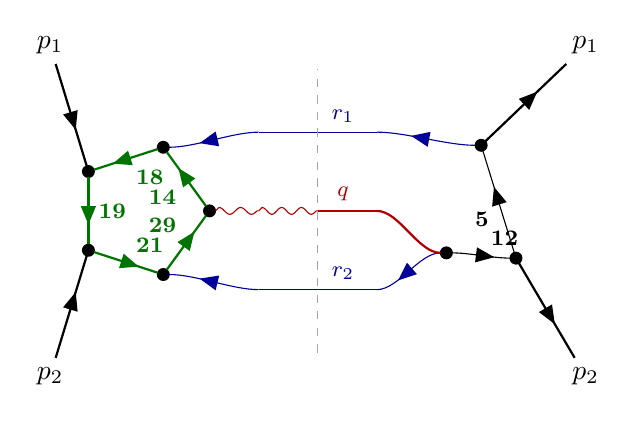
\begin{tikzpicture}
\begin{feynman}
\vertex (Lp1) at (-3.400,2.100) {$p_1$};
\vertex (Lp2) at (-3.400,-2.100) {$p_2$};
\vertex (Lcr1) at (-0.750,1.000);
\vertex (Lcr2) at (-0.750,-1.000);
\vertex (Lcq) at (-0.750,0.000);
\vertex (Mq) at (0,0.000);
\vertex[dot] (Lv0) at (-1.375,0.000) {};
\vertex[dot] (Lv1) at (-1.962,0.808) {};
\vertex[dot] (Lv2) at (-2.913,0.500) {};
\vertex[dot] (Lv3) at (-2.913,-0.500) {};
\vertex[dot] (Lv4) at (-1.962,-0.808) {};
\vertex (Rp1) at (3.400,2.100) {$p_1$};
\vertex (Rp2) at (3.400,-2.100) {$p_2$};
\vertex (Rcr1) at (0.750,1.000);
\vertex (Rcr2) at (0.750,-1.000);
\vertex (Rcq) at (0.750,0.000);
\vertex[dot] (R5) at (2.075,0.833) {};
\vertex[dot] (R12) at (2.517,-0.600) {};
\vertex[dot] (Rroot) at (1.633,-0.533) {};
\diagram* {
(Lv0) -- [plain, thick, green!45!black, with arrow=0.55, edge label={\footnotesize\bfseries 14}] (Lv1),
(Lv1) -- [plain, thick, green!45!black, with arrow=0.55, edge label={\footnotesize\bfseries 18}] (Lv2),
(Lv2) -- [plain, thick, green!45!black, with arrow=0.55, edge label={\footnotesize\bfseries 19}] (Lv3),
(Lv3) -- [plain, thick, green!45!black, with arrow=0.55, edge label={\footnotesize\bfseries 21}] (Lv4),
(Lv4) -- [plain, thick, green!45!black, with arrow=0.55, edge label={\footnotesize\bfseries 29}] (Lv0),
(Lcq) -- [boson, red!70!black] (Lv0),
(Lcr1) -- [plain, blue!60!black, out=180, in=0, looseness=0.75, with arrow=0.55] (Lv1),
(Lp1) -- [plain, thick, with arrow=0.55] (Lv2),
(Lp2) -- [plain, thick, with arrow=0.55] (Lv3),
(Lcr2) -- [plain, blue!60!black, out=180, in=0, looseness=0.75, with arrow=0.55] (Lv4),
(R12) -- [plain, with arrow=0.55, edge label={\footnotesize\bfseries 5}] (R5),
(Rroot) -- [plain, out=0, in=180, looseness=0.75, with arrow=0.55, edge label={\footnotesize\bfseries 12}] (R12),
(R5) -- [plain, thick, with arrow=0.55] (Rp1),
(R12) -- [plain, thick, with arrow=0.55] (Rp2),
(R5) -- [plain, blue!60!black, out=180, in=0, looseness=0.75, with arrow=0.55] (Rcr1),
(Rroot) -- [plain, blue!60!black, out=180, in=0, looseness=0.75, with arrow=0.55] (Rcr2),
(Rroot) -- [plain, red!70!black, double, double distance=1.2pt, thick, out=180, in=0, looseness=0.75] (Rcq),
(Rcr1) -- [plain, blue!60!black] (Lcr1),
(Rcr2) -- [plain, blue!60!black] (Lcr2),
(Rcq) -- [plain, red!70!black, double, double distance=1.2pt, thick] (Mq) -- [boson, red!70!black] (Lcq),
};
\end{feynman}
\draw[dashed, gray!70] (0,-1.80) -- (0,1.80);
\node[font=\footnotesize, blue!60!black, above] at (0.32,1.00) {$r_1$};
\node[font=\footnotesize, blue!60!black, above] at (0.32,-1.00) {$r_2$};
\node[font=\footnotesize, red!70!black, above] at (0.32,0.00) {$q$};
\end{tikzpicture}}\\[2mm]\textbf{topo21} (RR family 23, pentagon q-r1-p1-p2-r2)\\[2pt]{\footnotesize\begin{tabular}{@{}r@{\ \ }l@{\ \ }l@{}}\textbf{14} & $(k_1)^2$ & loop\\
\textbf{18} & $(k_1+r_1)^2$ & loop\\
\textbf{19} & $(k_1+p_1+r_1)^2$ & loop\\
\textbf{21} & $(k_1+p_1+p_2+r_1)^2$ & loop\\
\textbf{29} & $(k_1+p_1+p_2+r_1+r_2)^2$ & loop\\
\textbf{5} & $(p_1+r_1)^2$ & conjugate\\
\textbf{12} & $(p_1+p_2+r_1)^2$ & conjugate\\
\textbf{13} & $(p_1+p_2+r_2)^2$ & \textcolor{red}{irreducible numerator}\\\end{tabular}}\end{minipage}\hfill%
\begin{minipage}[t]{0.48\textwidth}\centering\resizebox{0.9\linewidth}{!}{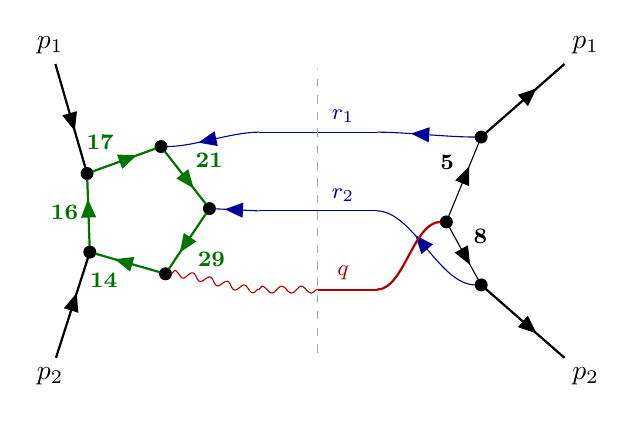
\begin{tikzpicture}
\begin{feynman}
\vertex (Lp1) at (-3.400,2.100) {$p_1$};
\vertex (Lp2) at (-3.400,-2.100) {$p_2$};
\vertex (Lcr1) at (-0.750,1.000);
\vertex (Lcr2) at (-0.750,0.000);
\vertex (Lcq) at (-0.750,-1.000);
\vertex (Mq) at (0,-1.000);
\vertex[dot] (Lv0) at (-1.934,-0.799) {};
\vertex[dot] (Lv1) at (-2.895,-0.523) {};
\vertex[dot] (Lv2) at (-2.930,0.475) {};
\vertex[dot] (Lv3) at (-1.991,0.817) {};
\vertex[dot] (Lv4) at (-1.376,0.030) {};
\vertex (Rp1) at (3.400,2.100) {$p_1$};
\vertex (Rp2) at (3.400,-2.100) {$p_2$};
\vertex (Rcr1) at (0.750,1.000);
\vertex (Rcr2) at (0.750,0.000);
\vertex (Rcq) at (0.750,-1.000);
\vertex[dot] (R5) at (2.075,0.938) {};
\vertex[dot] (Rroot) at (1.633,-0.140) {};
\vertex[dot] (R8) at (2.075,-0.940) {};
\diagram* {
(Lv0) -- [plain, thick, green!45!black, with arrow=0.55, edge label={\footnotesize\bfseries 14}] (Lv1),
(Lv1) -- [plain, thick, green!45!black, with arrow=0.55, edge label={\footnotesize\bfseries 16}] (Lv2),
(Lv2) -- [plain, thick, green!45!black, with arrow=0.55, edge label={\footnotesize\bfseries 17}] (Lv3),
(Lv3) -- [plain, thick, green!45!black, with arrow=0.55, edge label={\footnotesize\bfseries 21}] (Lv4),
(Lv4) -- [plain, thick, green!45!black, with arrow=0.55, edge label={\footnotesize\bfseries 29}] (Lv0),
(Lcq) -- [boson, red!70!black, out=180, in=0, looseness=0.75] (Lv0),
(Lp2) -- [plain, thick, with arrow=0.55] (Lv1),
(Lp1) -- [plain, thick, with arrow=0.55] (Lv2),
(Lcr1) -- [plain, blue!60!black, out=180, in=0, looseness=0.75, with arrow=0.55] (Lv3),
(Lcr2) -- [plain, blue!60!black, with arrow=0.55] (Lv4),
(Rroot) -- [plain, with arrow=0.55, edge label={\footnotesize\bfseries 5}] (R5),
(Rroot) -- [plain, with arrow=0.55, edge label={\footnotesize\bfseries 8}] (R8),
(R5) -- [plain, thick, with arrow=0.55] (Rp1),
(R8) -- [plain, thick, with arrow=0.55] (Rp2),
(R5) -- [plain, blue!60!black, out=180, in=0, looseness=0.75, with arrow=0.55] (Rcr1),
(R8) -- [plain, blue!60!black, out=180, in=0, looseness=0.75, with arrow=0.55] (Rcr2),
(Rroot) -- [plain, red!70!black, double, double distance=1.2pt, thick, out=180, in=0, looseness=0.75] (Rcq),
(Rcr1) -- [plain, blue!60!black] (Lcr1),
(Rcr2) -- [plain, blue!60!black] (Lcr2),
(Rcq) -- [plain, red!70!black, double, double distance=1.2pt, thick] (Mq) -- [boson, red!70!black] (Lcq),
};
\end{feynman}
\draw[dashed, gray!70] (0,-1.80) -- (0,1.80);
\node[font=\footnotesize, blue!60!black, above] at (0.32,1.00) {$r_1$};
\node[font=\footnotesize, blue!60!black, above] at (0.32,0.00) {$r_2$};
\node[font=\footnotesize, red!70!black, above] at (0.32,-1.00) {$q$};
\end{tikzpicture}}\\[2mm]\textbf{topo22} (RR family 7, pentagon q-p2-p1-r1-r2)\\[2pt]{\footnotesize\begin{tabular}{@{}r@{\ \ }l@{\ \ }l@{}}\textbf{14} & $(k_1)^2$ & loop\\
\textbf{16} & $(k_1+p_2)^2$ & loop\\
\textbf{17} & $(k_1+p_1+p_2)^2$ & loop\\
\textbf{21} & $(k_1+p_1+p_2+r_1)^2$ & loop\\
\textbf{29} & $(k_1+p_1+p_2+r_1+r_2)^2$ & loop\\
\textbf{5} & $(p_1+r_1)^2$ & conjugate\\
\textbf{8} & $(p_2+r_2)^2$ & conjugate\\
\textbf{10} & $(p_2+r_1+r_2)^2$ & \textcolor{red}{irreducible numerator}\\\end{tabular}}\end{minipage}

\bigskip

\begin{minipage}[t]{0.48\textwidth}\centering\resizebox{0.9\linewidth}{!}{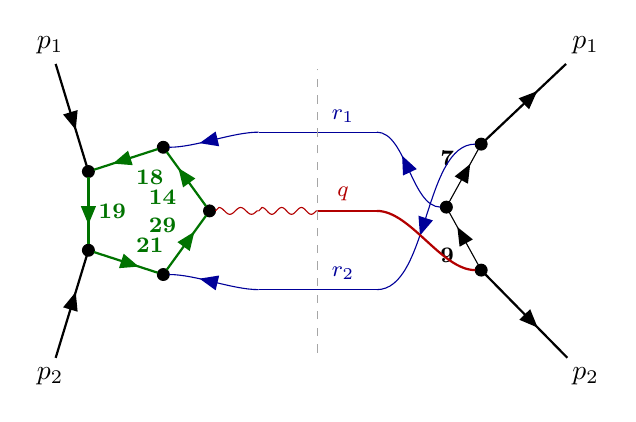
\begin{tikzpicture}
\begin{feynman}
\vertex (Lp1) at (-3.400,2.100) {$p_1$};
\vertex (Lp2) at (-3.400,-2.100) {$p_2$};
\vertex (Lcr1) at (-0.750,1.000);
\vertex (Lcr2) at (-0.750,-1.000);
\vertex (Lcq) at (-0.750,0.000);
\vertex (Mq) at (0,0.000);
\vertex[dot] (Lv0) at (-1.375,0.000) {};
\vertex[dot] (Lv1) at (-1.962,0.808) {};
\vertex[dot] (Lv2) at (-2.913,0.500) {};
\vertex[dot] (Lv3) at (-2.913,-0.500) {};
\vertex[dot] (Lv4) at (-1.962,-0.808) {};
\vertex (Rp1) at (3.400,2.100) {$p_1$};
\vertex (Rp2) at (3.400,-2.100) {$p_2$};
\vertex (Rcr1) at (0.750,1.000);
\vertex (Rcr2) at (0.750,-1.000);
\vertex (Rcq) at (0.750,0.000);
\vertex[dot] (R7) at (2.075,0.848) {};
\vertex[dot] (R9) at (1.633,0.048) {};
\vertex[dot] (Rroot) at (2.075,-0.752) {};
\diagram* {
(Lv0) -- [plain, thick, green!45!black, with arrow=0.55, edge label={\footnotesize\bfseries 14}] (Lv1),
(Lv1) -- [plain, thick, green!45!black, with arrow=0.55, edge label={\footnotesize\bfseries 18}] (Lv2),
(Lv2) -- [plain, thick, green!45!black, with arrow=0.55, edge label={\footnotesize\bfseries 19}] (Lv3),
(Lv3) -- [plain, thick, green!45!black, with arrow=0.55, edge label={\footnotesize\bfseries 21}] (Lv4),
(Lv4) -- [plain, thick, green!45!black, with arrow=0.55, edge label={\footnotesize\bfseries 29}] (Lv0),
(Lcq) -- [boson, red!70!black] (Lv0),
(Lcr1) -- [plain, blue!60!black, out=180, in=0, looseness=0.75, with arrow=0.55] (Lv1),
(Lp1) -- [plain, thick, with arrow=0.55] (Lv2),
(Lp2) -- [plain, thick, with arrow=0.55] (Lv3),
(Lcr2) -- [plain, blue!60!black, out=180, in=0, looseness=0.75, with arrow=0.55] (Lv4),
(R9) -- [plain, with arrow=0.55, edge label={\footnotesize\bfseries 7}] (R7),
(Rroot) -- [plain, with arrow=0.55, edge label={\footnotesize\bfseries 9}] (R9),
(R7) -- [plain, thick, with arrow=0.55] (Rp1),
(Rroot) -- [plain, thick, with arrow=0.55] (Rp2),
(R9) -- [plain, blue!60!black, out=180, in=0, looseness=0.75, with arrow=0.55] (Rcr1),
(R7) -- [plain, blue!60!black, out=180, in=0, looseness=0.75, with arrow=0.55] (Rcr2),
(Rroot) -- [plain, red!70!black, double, double distance=1.2pt, thick, out=180, in=0, looseness=0.75] (Rcq),
(Rcr1) -- [plain, blue!60!black] (Lcr1),
(Rcr2) -- [plain, blue!60!black] (Lcr2),
(Rcq) -- [plain, red!70!black, double, double distance=1.2pt, thick] (Mq) -- [boson, red!70!black] (Lcq),
};
\end{feynman}
\draw[dashed, gray!70] (0,-1.80) -- (0,1.80);
\node[font=\footnotesize, blue!60!black, above] at (0.32,1.00) {$r_1$};
\node[font=\footnotesize, blue!60!black, above] at (0.32,-1.00) {$r_2$};
\node[font=\footnotesize, red!70!black, above] at (0.32,0.00) {$q$};
\end{tikzpicture}}\\[2mm]\textbf{topo23} (RR family 33, pentagon q-r1-p1-p2-r2)\\[2pt]{\footnotesize\begin{tabular}{@{}r@{\ \ }l@{\ \ }l@{}}\textbf{14} & $(k_1)^2$ & loop\\
\textbf{18} & $(k_1+r_1)^2$ & loop\\
\textbf{19} & $(k_1+p_1+r_1)^2$ & loop\\
\textbf{21} & $(k_1+p_1+p_2+r_1)^2$ & loop\\
\textbf{29} & $(k_1+p_1+p_2+r_1+r_2)^2$ & loop\\
\textbf{7} & $(p_1+r_2)^2$ & conjugate\\
\textbf{9} & $(p_1+r_1+r_2)^2$ & conjugate\\
\textbf{13} & $(p_1+p_2+r_2)^2$ & \textcolor{red}{irreducible numerator}\\\end{tabular}}\end{minipage}\hfill%
\begin{minipage}[t]{0.48\textwidth}\centering\resizebox{0.9\linewidth}{!}{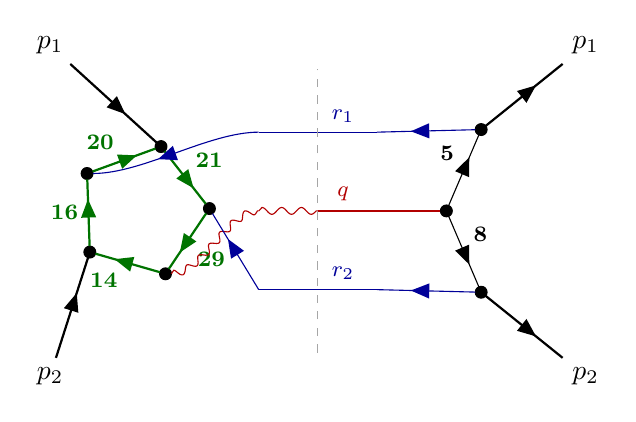
\begin{tikzpicture}
\begin{feynman}
\vertex (Lp1) at (-3.400,2.100) {$p_1$};
\vertex (Lp2) at (-3.400,-2.100) {$p_2$};
\vertex (Lcr1) at (-0.750,1.000);
\vertex (Lcr2) at (-0.750,-1.000);
\vertex (Lcq) at (-0.750,0.000);
\vertex (Mq) at (0,0.000);
\vertex[dot] (Lv0) at (-1.934,-0.799) {};
\vertex[dot] (Lv1) at (-2.895,-0.523) {};
\vertex[dot] (Lv2) at (-2.930,0.475) {};
\vertex[dot] (Lv3) at (-1.991,0.817) {};
\vertex[dot] (Lv4) at (-1.376,0.030) {};
\vertex (Rp1) at (3.400,2.100) {$p_1$};
\vertex (Rp2) at (3.400,-2.100) {$p_2$};
\vertex (Rcr1) at (0.750,1.000);
\vertex (Rcr2) at (0.750,-1.000);
\vertex (Rcq) at (0.750,0.000);
\vertex[dot] (R5) at (2.075,1.033) {};
\vertex[dot] (Rroot) at (1.633,0.000) {};
\vertex[dot] (R8) at (2.075,-1.033) {};
\diagram* {
(Lv0) -- [plain, thick, green!45!black, with arrow=0.55, edge label={\footnotesize\bfseries 14}] (Lv1),
(Lv1) -- [plain, thick, green!45!black, with arrow=0.55, edge label={\footnotesize\bfseries 16}] (Lv2),
(Lv2) -- [plain, thick, green!45!black, with arrow=0.55, edge label={\footnotesize\bfseries 20}] (Lv3),
(Lv3) -- [plain, thick, green!45!black, with arrow=0.55, edge label={\footnotesize\bfseries 21}] (Lv4),
(Lv4) -- [plain, thick, green!45!black, with arrow=0.55, edge label={\footnotesize\bfseries 29}] (Lv0),
(Lcq) -- [boson, red!70!black, out=180, in=0, looseness=0.75] (Lv0),
(Lp2) -- [plain, thick, with arrow=0.55] (Lv1),
(Lcr1) -- [plain, blue!60!black, out=180, in=0, looseness=0.75, with arrow=0.55] (Lv2),
(Lp1) -- [plain, thick, with arrow=0.55] (Lv3),
(Lcr2) -- [plain, blue!60!black, with arrow=0.55] (Lv4),
(Rroot) -- [plain, with arrow=0.55, edge label={\footnotesize\bfseries 5}] (R5),
(Rroot) -- [plain, with arrow=0.55, edge label={\footnotesize\bfseries 8}] (R8),
(R5) -- [plain, thick, with arrow=0.55] (Rp1),
(R8) -- [plain, thick, with arrow=0.55] (Rp2),
(R5) -- [plain, blue!60!black, with arrow=0.55] (Rcr1),
(R8) -- [plain, blue!60!black, with arrow=0.55] (Rcr2),
(Rroot) -- [plain, red!70!black, double, double distance=1.2pt, thick] (Rcq),
(Rcr1) -- [plain, blue!60!black] (Lcr1),
(Rcr2) -- [plain, blue!60!black] (Lcr2),
(Rcq) -- [plain, red!70!black, double, double distance=1.2pt, thick] (Mq) -- [boson, red!70!black] (Lcq),
};
\end{feynman}
\draw[dashed, gray!70] (0,-1.80) -- (0,1.80);
\node[font=\footnotesize, blue!60!black, above] at (0.32,1.00) {$r_1$};
\node[font=\footnotesize, blue!60!black, above] at (0.32,-1.00) {$r_2$};
\node[font=\footnotesize, red!70!black, above] at (0.32,0.00) {$q$};
\end{tikzpicture}}\\[2mm]\textbf{topo24} (RR family 6, pentagon q-p2-r1-p1-r2)\\[2pt]{\footnotesize\begin{tabular}{@{}r@{\ \ }l@{\ \ }l@{}}\textbf{14} & $(k_1)^2$ & loop\\
\textbf{16} & $(k_1+p_2)^2$ & loop\\
\textbf{20} & $(k_1+p_2+r_1)^2$ & loop\\
\textbf{21} & $(k_1+p_1+p_2+r_1)^2$ & loop\\
\textbf{29} & $(k_1+p_1+p_2+r_1+r_2)^2$ & loop\\
\textbf{5} & $(p_1+r_1)^2$ & conjugate\\
\textbf{8} & $(p_2+r_2)^2$ & conjugate\\
\textbf{9} & $(p_1+r_1+r_2)^2$ & \textcolor{red}{irreducible numerator}\\\end{tabular}}\end{minipage}

\bigskip

\begin{minipage}[t]{0.48\textwidth}\centering\resizebox{0.9\linewidth}{!}{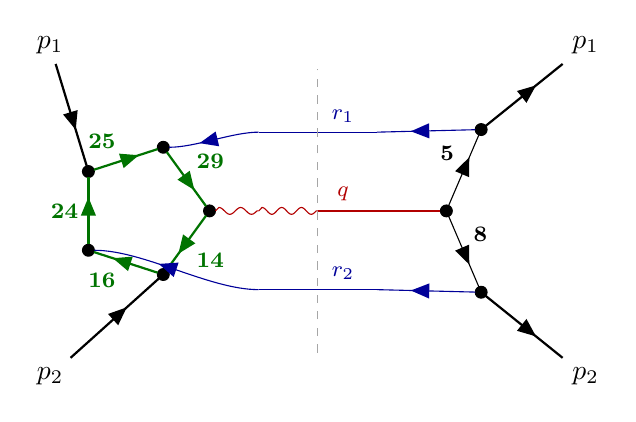
\begin{tikzpicture}
\begin{feynman}
\vertex (Lp1) at (-3.400,2.100) {$p_1$};
\vertex (Lp2) at (-3.400,-2.100) {$p_2$};
\vertex (Lcr1) at (-0.750,1.000);
\vertex (Lcr2) at (-0.750,-1.000);
\vertex (Lcq) at (-0.750,0.000);
\vertex (Mq) at (0,0.000);
\vertex[dot] (Lv0) at (-1.375,0.000) {};
\vertex[dot] (Lv1) at (-1.962,-0.808) {};
\vertex[dot] (Lv2) at (-2.913,-0.500) {};
\vertex[dot] (Lv3) at (-2.913,0.500) {};
\vertex[dot] (Lv4) at (-1.962,0.808) {};
\vertex (Rp1) at (3.400,2.100) {$p_1$};
\vertex (Rp2) at (3.400,-2.100) {$p_2$};
\vertex (Rcr1) at (0.750,1.000);
\vertex (Rcr2) at (0.750,-1.000);
\vertex (Rcq) at (0.750,0.000);
\vertex[dot] (R5) at (2.075,1.033) {};
\vertex[dot] (Rroot) at (1.633,0.000) {};
\vertex[dot] (R8) at (2.075,-1.033) {};
\diagram* {
(Lv0) -- [plain, thick, green!45!black, with arrow=0.55, edge label={\footnotesize\bfseries 14}] (Lv1),
(Lv1) -- [plain, thick, green!45!black, with arrow=0.55, edge label={\footnotesize\bfseries 16}] (Lv2),
(Lv2) -- [plain, thick, green!45!black, with arrow=0.55, edge label={\footnotesize\bfseries 24}] (Lv3),
(Lv3) -- [plain, thick, green!45!black, with arrow=0.55, edge label={\footnotesize\bfseries 25}] (Lv4),
(Lv4) -- [plain, thick, green!45!black, with arrow=0.55, edge label={\footnotesize\bfseries 29}] (Lv0),
(Lcq) -- [boson, red!70!black] (Lv0),
(Lp2) -- [plain, thick, with arrow=0.55] (Lv1),
(Lcr2) -- [plain, blue!60!black, out=180, in=0, looseness=0.75, with arrow=0.55] (Lv2),
(Lp1) -- [plain, thick, with arrow=0.55] (Lv3),
(Lcr1) -- [plain, blue!60!black, out=180, in=0, looseness=0.75, with arrow=0.55] (Lv4),
(Rroot) -- [plain, with arrow=0.55, edge label={\footnotesize\bfseries 5}] (R5),
(Rroot) -- [plain, with arrow=0.55, edge label={\footnotesize\bfseries 8}] (R8),
(R5) -- [plain, thick, with arrow=0.55] (Rp1),
(R8) -- [plain, thick, with arrow=0.55] (Rp2),
(R5) -- [plain, blue!60!black, with arrow=0.55] (Rcr1),
(R8) -- [plain, blue!60!black, with arrow=0.55] (Rcr2),
(Rroot) -- [plain, red!70!black, double, double distance=1.2pt, thick] (Rcq),
(Rcr1) -- [plain, blue!60!black] (Lcr1),
(Rcr2) -- [plain, blue!60!black] (Lcr2),
(Rcq) -- [plain, red!70!black, double, double distance=1.2pt, thick] (Mq) -- [boson, red!70!black] (Lcq),
};
\end{feynman}
\draw[dashed, gray!70] (0,-1.80) -- (0,1.80);
\node[font=\footnotesize, blue!60!black, above] at (0.32,1.00) {$r_1$};
\node[font=\footnotesize, blue!60!black, above] at (0.32,-1.00) {$r_2$};
\node[font=\footnotesize, red!70!black, above] at (0.32,0.00) {$q$};
\end{tikzpicture}}\\[2mm]\textbf{topo25} (RR family 18, pentagon q-p2-r2-p1-r1)\\[2pt]{\footnotesize\begin{tabular}{@{}r@{\ \ }l@{\ \ }l@{}}\textbf{14} & $(k_1)^2$ & loop\\
\textbf{16} & $(k_1+p_2)^2$ & loop\\
\textbf{24} & $(k_1+p_2+r_2)^2$ & loop\\
\textbf{25} & $(k_1+p_1+p_2+r_2)^2$ & loop\\
\textbf{29} & $(k_1+p_1+p_2+r_1+r_2)^2$ & loop\\
\textbf{5} & $(p_1+r_1)^2$ & conjugate\\
\textbf{8} & $(p_2+r_2)^2$ & conjugate\\
\textbf{13} & $(p_1+p_2+r_2)^2$ & \textcolor{red}{irreducible numerator}\\\end{tabular}}\end{minipage}\hfill%
\begin{minipage}[t]{0.48\textwidth}\centering\resizebox{0.9\linewidth}{!}{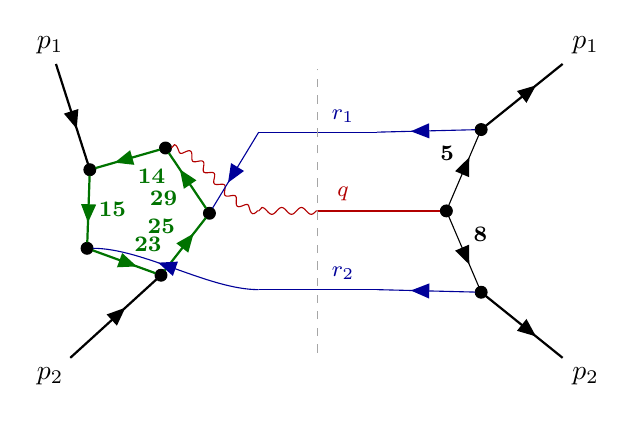
\begin{tikzpicture}
\begin{feynman}
\vertex (Lp1) at (-3.400,2.100) {$p_1$};
\vertex (Lp2) at (-3.400,-2.100) {$p_2$};
\vertex (Lcr1) at (-0.750,1.000);
\vertex (Lcr2) at (-0.750,-1.000);
\vertex (Lcq) at (-0.750,0.000);
\vertex (Mq) at (0,0.000);
\vertex[dot] (Lv0) at (-1.934,0.799) {};
\vertex[dot] (Lv1) at (-2.895,0.523) {};
\vertex[dot] (Lv2) at (-2.930,-0.475) {};
\vertex[dot] (Lv3) at (-1.991,-0.817) {};
\vertex[dot] (Lv4) at (-1.376,-0.030) {};
\vertex (Rp1) at (3.400,2.100) {$p_1$};
\vertex (Rp2) at (3.400,-2.100) {$p_2$};
\vertex (Rcr1) at (0.750,1.000);
\vertex (Rcr2) at (0.750,-1.000);
\vertex (Rcq) at (0.750,0.000);
\vertex[dot] (R5) at (2.075,1.033) {};
\vertex[dot] (Rroot) at (1.633,0.000) {};
\vertex[dot] (R8) at (2.075,-1.033) {};
\diagram* {
(Lv0) -- [plain, thick, green!45!black, with arrow=0.55, edge label={\footnotesize\bfseries 14}] (Lv1),
(Lv1) -- [plain, thick, green!45!black, with arrow=0.55, edge label={\footnotesize\bfseries 15}] (Lv2),
(Lv2) -- [plain, thick, green!45!black, with arrow=0.55, edge label={\footnotesize\bfseries 23}] (Lv3),
(Lv3) -- [plain, thick, green!45!black, with arrow=0.55, edge label={\footnotesize\bfseries 25}] (Lv4),
(Lv4) -- [plain, thick, green!45!black, with arrow=0.55, edge label={\footnotesize\bfseries 29}] (Lv0),
(Lcq) -- [boson, red!70!black, out=180, in=0, looseness=0.75] (Lv0),
(Lp1) -- [plain, thick, with arrow=0.55] (Lv1),
(Lcr2) -- [plain, blue!60!black, out=180, in=0, looseness=0.75, with arrow=0.55] (Lv2),
(Lp2) -- [plain, thick, with arrow=0.55] (Lv3),
(Lcr1) -- [plain, blue!60!black, with arrow=0.55] (Lv4),
(Rroot) -- [plain, with arrow=0.55, edge label={\footnotesize\bfseries 5}] (R5),
(Rroot) -- [plain, with arrow=0.55, edge label={\footnotesize\bfseries 8}] (R8),
(R5) -- [plain, thick, with arrow=0.55] (Rp1),
(R8) -- [plain, thick, with arrow=0.55] (Rp2),
(R5) -- [plain, blue!60!black, with arrow=0.55] (Rcr1),
(R8) -- [plain, blue!60!black, with arrow=0.55] (Rcr2),
(Rroot) -- [plain, red!70!black, double, double distance=1.2pt, thick] (Rcq),
(Rcr1) -- [plain, blue!60!black] (Lcr1),
(Rcr2) -- [plain, blue!60!black] (Lcr2),
(Rcq) -- [plain, red!70!black, double, double distance=1.2pt, thick] (Mq) -- [boson, red!70!black] (Lcq),
};
\end{feynman}
\draw[dashed, gray!70] (0,-1.80) -- (0,1.80);
\node[font=\footnotesize, blue!60!black, above] at (0.32,1.00) {$r_1$};
\node[font=\footnotesize, blue!60!black, above] at (0.32,-1.00) {$r_2$};
\node[font=\footnotesize, red!70!black, above] at (0.32,0.00) {$q$};
\end{tikzpicture}}\\[2mm]\textbf{topo26} (RR family 17, pentagon q-p1-r2-p2-r1)\\[2pt]{\footnotesize\begin{tabular}{@{}r@{\ \ }l@{\ \ }l@{}}\textbf{14} & $(k_1)^2$ & loop\\
\textbf{15} & $(k_1+p_1)^2$ & loop\\
\textbf{23} & $(k_1+p_1+r_2)^2$ & loop\\
\textbf{25} & $(k_1+p_1+p_2+r_2)^2$ & loop\\
\textbf{29} & $(k_1+p_1+p_2+r_1+r_2)^2$ & loop\\
\textbf{5} & $(p_1+r_1)^2$ & conjugate\\
\textbf{8} & $(p_2+r_2)^2$ & conjugate\\
\textbf{12} & $(p_1+p_2+r_1)^2$ & \textcolor{red}{irreducible numerator}\\\end{tabular}}\end{minipage}

\bigskip

\begin{minipage}[t]{0.48\textwidth}\centering\resizebox{0.9\linewidth}{!}{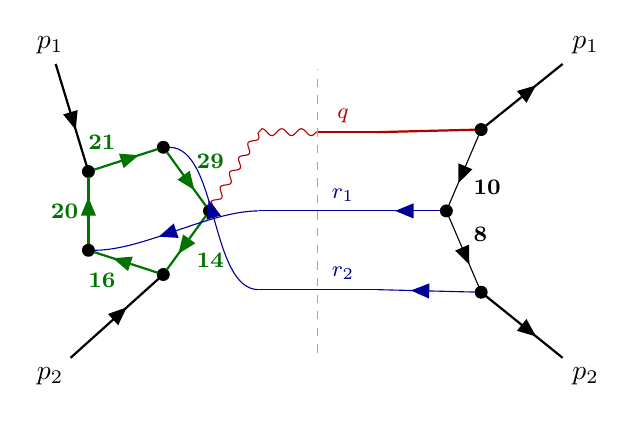
\begin{tikzpicture}
\begin{feynman}
\vertex (Lp1) at (-3.400,2.100) {$p_1$};
\vertex (Lp2) at (-3.400,-2.100) {$p_2$};
\vertex (Lcr1) at (-0.750,0.000);
\vertex (Lcr2) at (-0.750,-1.000);
\vertex (Lcq) at (-0.750,1.000);
\vertex (Mq) at (0,1.000);
\vertex[dot] (Lv0) at (-1.375,0.000) {};
\vertex[dot] (Lv1) at (-1.962,-0.808) {};
\vertex[dot] (Lv2) at (-2.913,-0.500) {};
\vertex[dot] (Lv3) at (-2.913,0.500) {};
\vertex[dot] (Lv4) at (-1.962,0.808) {};
\vertex (Rp1) at (3.400,2.100) {$p_1$};
\vertex (Rp2) at (3.400,-2.100) {$p_2$};
\vertex (Rcr1) at (0.750,0.000);
\vertex (Rcr2) at (0.750,-1.000);
\vertex (Rcq) at (0.750,1.000);
\vertex[dot] (R8) at (2.075,-1.033) {};
\vertex[dot] (R10) at (1.633,0.000) {};
\vertex[dot] (Rroot) at (2.075,1.033) {};
\diagram* {
(Lv0) -- [plain, thick, green!45!black, with arrow=0.55, edge label={\footnotesize\bfseries 14}] (Lv1),
(Lv1) -- [plain, thick, green!45!black, with arrow=0.55, edge label={\footnotesize\bfseries 16}] (Lv2),
(Lv2) -- [plain, thick, green!45!black, with arrow=0.55, edge label={\footnotesize\bfseries 20}] (Lv3),
(Lv3) -- [plain, thick, green!45!black, with arrow=0.55, edge label={\footnotesize\bfseries 21}] (Lv4),
(Lv4) -- [plain, thick, green!45!black, with arrow=0.55, edge label={\footnotesize\bfseries 29}] (Lv0),
(Lcq) -- [boson, red!70!black] (Lv0),
(Lp2) -- [plain, thick, with arrow=0.55] (Lv1),
(Lcr1) -- [plain, blue!60!black, out=180, in=0, looseness=0.75, with arrow=0.55] (Lv2),
(Lp1) -- [plain, thick, with arrow=0.55] (Lv3),
(Lcr2) -- [plain, blue!60!black, out=180, in=0, looseness=0.75, with arrow=0.55] (Lv4),
(R10) -- [plain, with arrow=0.55, edge label={\footnotesize\bfseries 8}] (R8),
(Rroot) -- [plain, with arrow=0.55, edge label={\footnotesize\bfseries 10}] (R10),
(Rroot) -- [plain, thick, with arrow=0.55] (Rp1),
(R8) -- [plain, thick, with arrow=0.55] (Rp2),
(R10) -- [plain, blue!60!black, with arrow=0.55] (Rcr1),
(R8) -- [plain, blue!60!black, with arrow=0.55] (Rcr2),
(Rroot) -- [plain, red!70!black, double, double distance=1.2pt, thick] (Rcq),
(Rcr1) -- [plain, blue!60!black] (Lcr1),
(Rcr2) -- [plain, blue!60!black] (Lcr2),
(Rcq) -- [plain, red!70!black, double, double distance=1.2pt, thick] (Mq) -- [boson, red!70!black] (Lcq),
};
\end{feynman}
\draw[dashed, gray!70] (0,-1.80) -- (0,1.80);
\node[font=\footnotesize, blue!60!black, above] at (0.32,0.00) {$r_1$};
\node[font=\footnotesize, blue!60!black, above] at (0.32,-1.00) {$r_2$};
\node[font=\footnotesize, red!70!black, above] at (0.32,1.00) {$q$};
\end{tikzpicture}}\\[2mm]\textbf{topo27} (RR family 29, pentagon q-p2-r1-p1-r2)\\[2pt]{\footnotesize\begin{tabular}{@{}r@{\ \ }l@{\ \ }l@{}}\textbf{14} & $(k_1)^2$ & loop\\
\textbf{16} & $(k_1+p_2)^2$ & loop\\
\textbf{20} & $(k_1+p_2+r_1)^2$ & loop\\
\textbf{21} & $(k_1+p_1+p_2+r_1)^2$ & loop\\
\textbf{29} & $(k_1+p_1+p_2+r_1+r_2)^2$ & loop\\
\textbf{8} & $(p_2+r_2)^2$ & conjugate\\
\textbf{10} & $(p_2+r_1+r_2)^2$ & conjugate\\
\textbf{13} & $(p_1+p_2+r_2)^2$ & \textcolor{red}{irreducible numerator}\\\end{tabular}}\end{minipage}\hfill%
\begin{minipage}[t]{0.48\textwidth}\centering\resizebox{0.9\linewidth}{!}{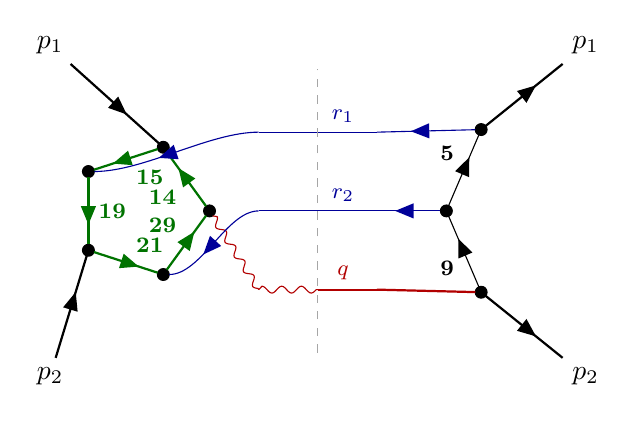
\begin{tikzpicture}
\begin{feynman}
\vertex (Lp1) at (-3.400,2.100) {$p_1$};
\vertex (Lp2) at (-3.400,-2.100) {$p_2$};
\vertex (Lcr1) at (-0.750,1.000);
\vertex (Lcr2) at (-0.750,0.000);
\vertex (Lcq) at (-0.750,-1.000);
\vertex (Mq) at (0,-1.000);
\vertex[dot] (Lv0) at (-1.375,0.000) {};
\vertex[dot] (Lv1) at (-1.962,0.808) {};
\vertex[dot] (Lv2) at (-2.913,0.500) {};
\vertex[dot] (Lv3) at (-2.913,-0.500) {};
\vertex[dot] (Lv4) at (-1.962,-0.808) {};
\vertex (Rp1) at (3.400,2.100) {$p_1$};
\vertex (Rp2) at (3.400,-2.100) {$p_2$};
\vertex (Rcr1) at (0.750,1.000);
\vertex (Rcr2) at (0.750,0.000);
\vertex (Rcq) at (0.750,-1.000);
\vertex[dot] (R5) at (2.075,1.033) {};
\vertex[dot] (R9) at (1.633,0.000) {};
\vertex[dot] (Rroot) at (2.075,-1.033) {};
\diagram* {
(Lv0) -- [plain, thick, green!45!black, with arrow=0.55, edge label={\footnotesize\bfseries 14}] (Lv1),
(Lv1) -- [plain, thick, green!45!black, with arrow=0.55, edge label={\footnotesize\bfseries 15}] (Lv2),
(Lv2) -- [plain, thick, green!45!black, with arrow=0.55, edge label={\footnotesize\bfseries 19}] (Lv3),
(Lv3) -- [plain, thick, green!45!black, with arrow=0.55, edge label={\footnotesize\bfseries 21}] (Lv4),
(Lv4) -- [plain, thick, green!45!black, with arrow=0.55, edge label={\footnotesize\bfseries 29}] (Lv0),
(Lcq) -- [boson, red!70!black] (Lv0),
(Lp1) -- [plain, thick, with arrow=0.55] (Lv1),
(Lcr1) -- [plain, blue!60!black, out=180, in=0, looseness=0.75, with arrow=0.55] (Lv2),
(Lp2) -- [plain, thick, with arrow=0.55] (Lv3),
(Lcr2) -- [plain, blue!60!black, out=180, in=0, looseness=0.75, with arrow=0.55] (Lv4),
(R9) -- [plain, with arrow=0.55, edge label={\footnotesize\bfseries 5}] (R5),
(Rroot) -- [plain, with arrow=0.55, edge label={\footnotesize\bfseries 9}] (R9),
(R5) -- [plain, thick, with arrow=0.55] (Rp1),
(Rroot) -- [plain, thick, with arrow=0.55] (Rp2),
(R5) -- [plain, blue!60!black, with arrow=0.55] (Rcr1),
(R9) -- [plain, blue!60!black, with arrow=0.55] (Rcr2),
(Rroot) -- [plain, red!70!black, double, double distance=1.2pt, thick] (Rcq),
(Rcr1) -- [plain, blue!60!black] (Lcr1),
(Rcr2) -- [plain, blue!60!black] (Lcr2),
(Rcq) -- [plain, red!70!black, double, double distance=1.2pt, thick] (Mq) -- [boson, red!70!black] (Lcq),
};
\end{feynman}
\draw[dashed, gray!70] (0,-1.80) -- (0,1.80);
\node[font=\footnotesize, blue!60!black, above] at (0.32,1.00) {$r_1$};
\node[font=\footnotesize, blue!60!black, above] at (0.32,0.00) {$r_2$};
\node[font=\footnotesize, red!70!black, above] at (0.32,-1.00) {$q$};
\end{tikzpicture}}\\[2mm]\textbf{topo28} (RR family 3, pentagon q-p1-r1-p2-r2)\\[2pt]{\footnotesize\begin{tabular}{@{}r@{\ \ }l@{\ \ }l@{}}\textbf{14} & $(k_1)^2$ & loop\\
\textbf{15} & $(k_1+p_1)^2$ & loop\\
\textbf{19} & $(k_1+p_1+r_1)^2$ & loop\\
\textbf{21} & $(k_1+p_1+p_2+r_1)^2$ & loop\\
\textbf{29} & $(k_1+p_1+p_2+r_1+r_2)^2$ & loop\\
\textbf{5} & $(p_1+r_1)^2$ & conjugate\\
\textbf{9} & $(p_1+r_1+r_2)^2$ & conjugate\\
\textbf{6} & $(p_2+r_1)^2$ & \textcolor{red}{irreducible numerator}\\\end{tabular}}\end{minipage}

\bigskip

\begin{minipage}[t]{0.48\textwidth}\centering\resizebox{0.9\linewidth}{!}{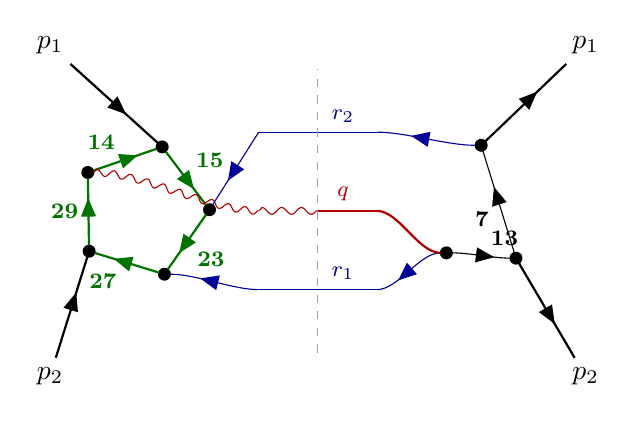
\begin{tikzpicture}
\begin{feynman}
\vertex (Lp1) at (-3.400,2.100) {$p_1$};
\vertex (Lp2) at (-3.400,-2.100) {$p_2$};
\vertex (Lcr1) at (-0.750,-1.000);
\vertex (Lcr2) at (-0.750,1.000);
\vertex (Lcq) at (-0.750,0.000);
\vertex (Mq) at (0,0.000);
\vertex[dot] (Lv0) at (-2.921,0.488) {};
\vertex[dot] (Lv1) at (-1.976,0.813) {};
\vertex[dot] (Lv2) at (-1.375,0.015) {};
\vertex[dot] (Lv3) at (-1.948,-0.804) {};
\vertex[dot] (Lv4) at (-2.904,-0.512) {};
\vertex (Rp1) at (3.400,2.100) {$p_1$};
\vertex (Rp2) at (3.400,-2.100) {$p_2$};
\vertex (Rcr1) at (0.750,-1.000);
\vertex (Rcr2) at (0.750,1.000);
\vertex (Rcq) at (0.750,0.000);
\vertex[dot] (R7) at (2.075,0.833) {};
\vertex[dot] (R13) at (2.517,-0.600) {};
\vertex[dot] (Rroot) at (1.633,-0.533) {};
\diagram* {
(Lv0) -- [plain, thick, green!45!black, with arrow=0.55, edge label={\footnotesize\bfseries 14}] (Lv1),
(Lv1) -- [plain, thick, green!45!black, with arrow=0.55, edge label={\footnotesize\bfseries 15}] (Lv2),
(Lv2) -- [plain, thick, green!45!black, with arrow=0.55, edge label={\footnotesize\bfseries 23}] (Lv3),
(Lv3) -- [plain, thick, green!45!black, with arrow=0.55, edge label={\footnotesize\bfseries 27}] (Lv4),
(Lv4) -- [plain, thick, green!45!black, with arrow=0.55, edge label={\footnotesize\bfseries 29}] (Lv0),
(Lcq) -- [boson, red!70!black, out=180, in=0, looseness=0.75] (Lv0),
(Lp1) -- [plain, thick, with arrow=0.55] (Lv1),
(Lcr2) -- [plain, blue!60!black, with arrow=0.55] (Lv2),
(Lcr1) -- [plain, blue!60!black, out=180, in=0, looseness=0.75, with arrow=0.55] (Lv3),
(Lp2) -- [plain, thick, with arrow=0.55] (Lv4),
(R13) -- [plain, with arrow=0.55, edge label={\footnotesize\bfseries 7}] (R7),
(Rroot) -- [plain, out=0, in=180, looseness=0.75, with arrow=0.55, edge label={\footnotesize\bfseries 13}] (R13),
(R7) -- [plain, thick, with arrow=0.55] (Rp1),
(R13) -- [plain, thick, with arrow=0.55] (Rp2),
(Rroot) -- [plain, blue!60!black, out=180, in=0, looseness=0.75, with arrow=0.55] (Rcr1),
(R7) -- [plain, blue!60!black, out=180, in=0, looseness=0.75, with arrow=0.55] (Rcr2),
(Rroot) -- [plain, red!70!black, double, double distance=1.2pt, thick, out=180, in=0, looseness=0.75] (Rcq),
(Rcr1) -- [plain, blue!60!black] (Lcr1),
(Rcr2) -- [plain, blue!60!black] (Lcr2),
(Rcq) -- [plain, red!70!black, double, double distance=1.2pt, thick] (Mq) -- [boson, red!70!black] (Lcq),
};
\end{feynman}
\draw[dashed, gray!70] (0,-1.80) -- (0,1.80);
\node[font=\footnotesize, blue!60!black, above] at (0.32,-1.00) {$r_1$};
\node[font=\footnotesize, blue!60!black, above] at (0.32,1.00) {$r_2$};
\node[font=\footnotesize, red!70!black, above] at (0.32,0.00) {$q$};
\end{tikzpicture}}\\[2mm]\textbf{topo29} (RR family 30, pentagon q-p1-r2-r1-p2)\\[2pt]{\footnotesize\begin{tabular}{@{}r@{\ \ }l@{\ \ }l@{}}\textbf{14} & $(k_1)^2$ & loop\\
\textbf{15} & $(k_1+p_1)^2$ & loop\\
\textbf{23} & $(k_1+p_1+r_2)^2$ & loop\\
\textbf{27} & $(k_1+p_1+r_1+r_2)^2$ & loop\\
\textbf{29} & $(k_1+p_1+p_2+r_1+r_2)^2$ & loop\\
\textbf{7} & $(p_1+r_2)^2$ & conjugate\\
\textbf{13} & $(p_1+p_2+r_2)^2$ & conjugate\\
\textbf{11} & $(r_1+r_2)^2$ & \textcolor{red}{irreducible numerator}\\\end{tabular}}\end{minipage}\hfill%
\begin{minipage}[t]{0.48\textwidth}\centering\resizebox{0.9\linewidth}{!}{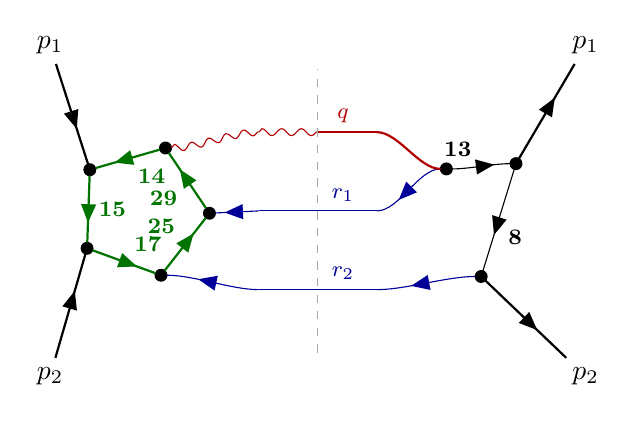
\begin{tikzpicture}
\begin{feynman}
\vertex (Lp1) at (-3.400,2.100) {$p_1$};
\vertex (Lp2) at (-3.400,-2.100) {$p_2$};
\vertex (Lcr1) at (-0.750,0.000);
\vertex (Lcr2) at (-0.750,-1.000);
\vertex (Lcq) at (-0.750,1.000);
\vertex (Mq) at (0,1.000);
\vertex[dot] (Lv0) at (-1.934,0.799) {};
\vertex[dot] (Lv1) at (-2.895,0.523) {};
\vertex[dot] (Lv2) at (-2.930,-0.475) {};
\vertex[dot] (Lv3) at (-1.991,-0.817) {};
\vertex[dot] (Lv4) at (-1.376,-0.030) {};
\vertex (Rp1) at (3.400,2.100) {$p_1$};
\vertex (Rp2) at (3.400,-2.100) {$p_2$};
\vertex (Rcr1) at (0.750,0.000);
\vertex (Rcr2) at (0.750,-1.000);
\vertex (Rcq) at (0.750,1.000);
\vertex[dot] (R8) at (2.075,-0.833) {};
\vertex[dot] (R13) at (2.517,0.600) {};
\vertex[dot] (Rroot) at (1.633,0.533) {};
\diagram* {
(Lv0) -- [plain, thick, green!45!black, with arrow=0.55, edge label={\footnotesize\bfseries 14}] (Lv1),
(Lv1) -- [plain, thick, green!45!black, with arrow=0.55, edge label={\footnotesize\bfseries 15}] (Lv2),
(Lv2) -- [plain, thick, green!45!black, with arrow=0.55, edge label={\footnotesize\bfseries 17}] (Lv3),
(Lv3) -- [plain, thick, green!45!black, with arrow=0.55, edge label={\footnotesize\bfseries 25}] (Lv4),
(Lv4) -- [plain, thick, green!45!black, with arrow=0.55, edge label={\footnotesize\bfseries 29}] (Lv0),
(Lcq) -- [boson, red!70!black, out=180, in=0, looseness=0.75] (Lv0),
(Lp1) -- [plain, thick, with arrow=0.55] (Lv1),
(Lp2) -- [plain, thick, with arrow=0.55] (Lv2),
(Lcr2) -- [plain, blue!60!black, out=180, in=0, looseness=0.75, with arrow=0.55] (Lv3),
(Lcr1) -- [plain, blue!60!black, with arrow=0.55] (Lv4),
(R13) -- [plain, with arrow=0.55, edge label={\footnotesize\bfseries 8}] (R8),
(Rroot) -- [plain, out=0, in=180, looseness=0.75, with arrow=0.55, edge label={\footnotesize\bfseries 13}] (R13),
(R13) -- [plain, thick, with arrow=0.55] (Rp1),
(R8) -- [plain, thick, with arrow=0.55] (Rp2),
(Rroot) -- [plain, blue!60!black, out=180, in=0, looseness=0.75, with arrow=0.55] (Rcr1),
(R8) -- [plain, blue!60!black, out=180, in=0, looseness=0.75, with arrow=0.55] (Rcr2),
(Rroot) -- [plain, red!70!black, double, double distance=1.2pt, thick, out=180, in=0, looseness=0.75] (Rcq),
(Rcr1) -- [plain, blue!60!black] (Lcr1),
(Rcr2) -- [plain, blue!60!black] (Lcr2),
(Rcq) -- [plain, red!70!black, double, double distance=1.2pt, thick] (Mq) -- [boson, red!70!black] (Lcq),
};
\end{feynman}
\draw[dashed, gray!70] (0,-1.80) -- (0,1.80);
\node[font=\footnotesize, blue!60!black, above] at (0.32,0.00) {$r_1$};
\node[font=\footnotesize, blue!60!black, above] at (0.32,-1.00) {$r_2$};
\node[font=\footnotesize, red!70!black, above] at (0.32,1.00) {$q$};
\end{tikzpicture}}\\[2mm]\textbf{topo30} (RR family 31, pentagon q-p1-p2-r2-r1)\\[2pt]{\footnotesize\begin{tabular}{@{}r@{\ \ }l@{\ \ }l@{}}\textbf{14} & $(k_1)^2$ & loop\\
\textbf{15} & $(k_1+p_1)^2$ & loop\\
\textbf{17} & $(k_1+p_1+p_2)^2$ & loop\\
\textbf{25} & $(k_1+p_1+p_2+r_2)^2$ & loop\\
\textbf{29} & $(k_1+p_1+p_2+r_1+r_2)^2$ & loop\\
\textbf{8} & $(p_2+r_2)^2$ & conjugate\\
\textbf{13} & $(p_1+p_2+r_2)^2$ & conjugate\\
\textbf{11} & $(r_1+r_2)^2$ & \textcolor{red}{irreducible numerator}\\\end{tabular}}\end{minipage}

\bigskip

\begin{minipage}[t]{0.48\textwidth}\centering\resizebox{0.9\linewidth}{!}{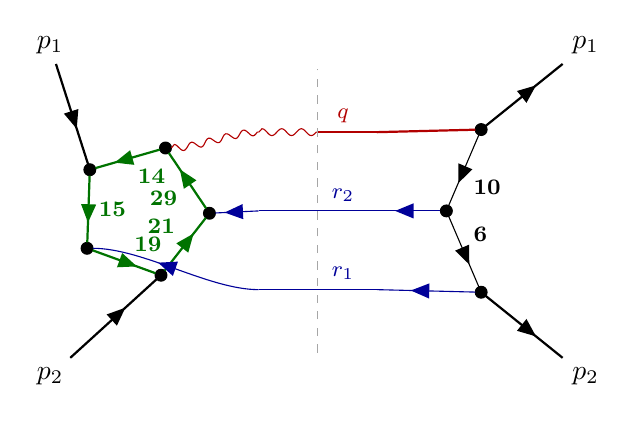
\begin{tikzpicture}
\begin{feynman}
\vertex (Lp1) at (-3.400,2.100) {$p_1$};
\vertex (Lp2) at (-3.400,-2.100) {$p_2$};
\vertex (Lcr1) at (-0.750,-1.000);
\vertex (Lcr2) at (-0.750,0.000);
\vertex (Lcq) at (-0.750,1.000);
\vertex (Mq) at (0,1.000);
\vertex[dot] (Lv0) at (-1.934,0.799) {};
\vertex[dot] (Lv1) at (-2.895,0.523) {};
\vertex[dot] (Lv2) at (-2.930,-0.475) {};
\vertex[dot] (Lv3) at (-1.991,-0.817) {};
\vertex[dot] (Lv4) at (-1.376,-0.030) {};
\vertex (Rp1) at (3.400,2.100) {$p_1$};
\vertex (Rp2) at (3.400,-2.100) {$p_2$};
\vertex (Rcr1) at (0.750,-1.000);
\vertex (Rcr2) at (0.750,0.000);
\vertex (Rcq) at (0.750,1.000);
\vertex[dot] (R6) at (2.075,-1.033) {};
\vertex[dot] (R10) at (1.633,0.000) {};
\vertex[dot] (Rroot) at (2.075,1.033) {};
\diagram* {
(Lv0) -- [plain, thick, green!45!black, with arrow=0.55, edge label={\footnotesize\bfseries 14}] (Lv1),
(Lv1) -- [plain, thick, green!45!black, with arrow=0.55, edge label={\footnotesize\bfseries 15}] (Lv2),
(Lv2) -- [plain, thick, green!45!black, with arrow=0.55, edge label={\footnotesize\bfseries 19}] (Lv3),
(Lv3) -- [plain, thick, green!45!black, with arrow=0.55, edge label={\footnotesize\bfseries 21}] (Lv4),
(Lv4) -- [plain, thick, green!45!black, with arrow=0.55, edge label={\footnotesize\bfseries 29}] (Lv0),
(Lcq) -- [boson, red!70!black, out=180, in=0, looseness=0.75] (Lv0),
(Lp1) -- [plain, thick, with arrow=0.55] (Lv1),
(Lcr1) -- [plain, blue!60!black, out=180, in=0, looseness=0.75, with arrow=0.55] (Lv2),
(Lp2) -- [plain, thick, with arrow=0.55] (Lv3),
(Lcr2) -- [plain, blue!60!black, with arrow=0.55] (Lv4),
(R10) -- [plain, with arrow=0.55, edge label={\footnotesize\bfseries 6}] (R6),
(Rroot) -- [plain, with arrow=0.55, edge label={\footnotesize\bfseries 10}] (R10),
(Rroot) -- [plain, thick, with arrow=0.55] (Rp1),
(R6) -- [plain, thick, with arrow=0.55] (Rp2),
(R6) -- [plain, blue!60!black, with arrow=0.55] (Rcr1),
(R10) -- [plain, blue!60!black, with arrow=0.55] (Rcr2),
(Rroot) -- [plain, red!70!black, double, double distance=1.2pt, thick] (Rcq),
(Rcr1) -- [plain, blue!60!black] (Lcr1),
(Rcr2) -- [plain, blue!60!black] (Lcr2),
(Rcq) -- [plain, red!70!black, double, double distance=1.2pt, thick] (Mq) -- [boson, red!70!black] (Lcq),
};
\end{feynman}
\draw[dashed, gray!70] (0,-1.80) -- (0,1.80);
\node[font=\footnotesize, blue!60!black, above] at (0.32,-1.00) {$r_1$};
\node[font=\footnotesize, blue!60!black, above] at (0.32,0.00) {$r_2$};
\node[font=\footnotesize, red!70!black, above] at (0.32,1.00) {$q$};
\end{tikzpicture}}\\[2mm]\textbf{topo31} (RR family 4, pentagon q-p1-r1-p2-r2)\\[2pt]{\footnotesize\begin{tabular}{@{}r@{\ \ }l@{\ \ }l@{}}\textbf{14} & $(k_1)^2$ & loop\\
\textbf{15} & $(k_1+p_1)^2$ & loop\\
\textbf{19} & $(k_1+p_1+r_1)^2$ & loop\\
\textbf{21} & $(k_1+p_1+p_2+r_1)^2$ & loop\\
\textbf{29} & $(k_1+p_1+p_2+r_1+r_2)^2$ & loop\\
\textbf{6} & $(p_2+r_1)^2$ & conjugate\\
\textbf{10} & $(p_2+r_1+r_2)^2$ & conjugate\\
\textbf{5} & $(p_1+r_1)^2$ & \textcolor{red}{irreducible numerator}\\\end{tabular}}\end{minipage}\hfill%
\begin{minipage}[t]{0.48\textwidth}\centering\resizebox{0.9\linewidth}{!}{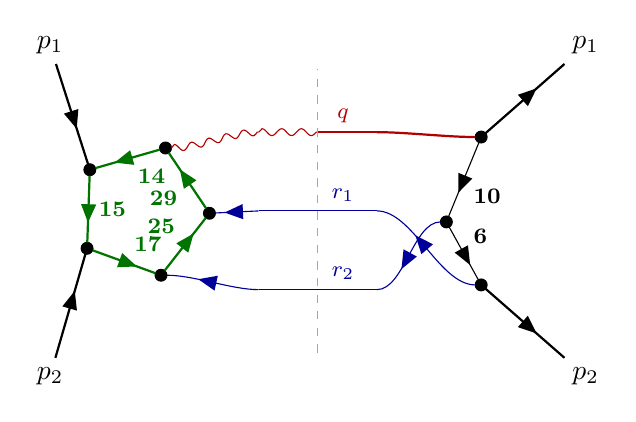
\begin{tikzpicture}
\begin{feynman}
\vertex (Lp1) at (-3.400,2.100) {$p_1$};
\vertex (Lp2) at (-3.400,-2.100) {$p_2$};
\vertex (Lcr1) at (-0.750,0.000);
\vertex (Lcr2) at (-0.750,-1.000);
\vertex (Lcq) at (-0.750,1.000);
\vertex (Mq) at (0,1.000);
\vertex[dot] (Lv0) at (-1.934,0.799) {};
\vertex[dot] (Lv1) at (-2.895,0.523) {};
\vertex[dot] (Lv2) at (-2.930,-0.475) {};
\vertex[dot] (Lv3) at (-1.991,-0.817) {};
\vertex[dot] (Lv4) at (-1.376,-0.030) {};
\vertex (Rp1) at (3.400,2.100) {$p_1$};
\vertex (Rp2) at (3.400,-2.100) {$p_2$};
\vertex (Rcr1) at (0.750,0.000);
\vertex (Rcr2) at (0.750,-1.000);
\vertex (Rcq) at (0.750,1.000);
\vertex[dot] (R6) at (2.075,-0.940) {};
\vertex[dot] (R10) at (1.633,-0.140) {};
\vertex[dot] (Rroot) at (2.075,0.938) {};
\diagram* {
(Lv0) -- [plain, thick, green!45!black, with arrow=0.55, edge label={\footnotesize\bfseries 14}] (Lv1),
(Lv1) -- [plain, thick, green!45!black, with arrow=0.55, edge label={\footnotesize\bfseries 15}] (Lv2),
(Lv2) -- [plain, thick, green!45!black, with arrow=0.55, edge label={\footnotesize\bfseries 17}] (Lv3),
(Lv3) -- [plain, thick, green!45!black, with arrow=0.55, edge label={\footnotesize\bfseries 25}] (Lv4),
(Lv4) -- [plain, thick, green!45!black, with arrow=0.55, edge label={\footnotesize\bfseries 29}] (Lv0),
(Lcq) -- [boson, red!70!black, out=180, in=0, looseness=0.75] (Lv0),
(Lp1) -- [plain, thick, with arrow=0.55] (Lv1),
(Lp2) -- [plain, thick, with arrow=0.55] (Lv2),
(Lcr2) -- [plain, blue!60!black, out=180, in=0, looseness=0.75, with arrow=0.55] (Lv3),
(Lcr1) -- [plain, blue!60!black, with arrow=0.55] (Lv4),
(R10) -- [plain, with arrow=0.55, edge label={\footnotesize\bfseries 6}] (R6),
(Rroot) -- [plain, with arrow=0.55, edge label={\footnotesize\bfseries 10}] (R10),
(Rroot) -- [plain, thick, with arrow=0.55] (Rp1),
(R6) -- [plain, thick, with arrow=0.55] (Rp2),
(R6) -- [plain, blue!60!black, out=180, in=0, looseness=0.75, with arrow=0.55] (Rcr1),
(R10) -- [plain, blue!60!black, out=180, in=0, looseness=0.75, with arrow=0.55] (Rcr2),
(Rroot) -- [plain, red!70!black, double, double distance=1.2pt, thick, out=180, in=0, looseness=0.75] (Rcq),
(Rcr1) -- [plain, blue!60!black] (Lcr1),
(Rcr2) -- [plain, blue!60!black] (Lcr2),
(Rcq) -- [plain, red!70!black, double, double distance=1.2pt, thick] (Mq) -- [boson, red!70!black] (Lcq),
};
\end{feynman}
\draw[dashed, gray!70] (0,-1.80) -- (0,1.80);
\node[font=\footnotesize, blue!60!black, above] at (0.32,0.00) {$r_1$};
\node[font=\footnotesize, blue!60!black, above] at (0.32,-1.00) {$r_2$};
\node[font=\footnotesize, red!70!black, above] at (0.32,1.00) {$q$};
\end{tikzpicture}}\\[2mm]\textbf{topo32} (RR family 27, pentagon q-p1-p2-r2-r1)\\[2pt]{\footnotesize\begin{tabular}{@{}r@{\ \ }l@{\ \ }l@{}}\textbf{14} & $(k_1)^2$ & loop\\
\textbf{15} & $(k_1+p_1)^2$ & loop\\
\textbf{17} & $(k_1+p_1+p_2)^2$ & loop\\
\textbf{25} & $(k_1+p_1+p_2+r_2)^2$ & loop\\
\textbf{29} & $(k_1+p_1+p_2+r_1+r_2)^2$ & loop\\
\textbf{6} & $(p_2+r_1)^2$ & conjugate\\
\textbf{10} & $(p_2+r_1+r_2)^2$ & conjugate\\
\textbf{13} & $(p_1+p_2+r_2)^2$ & \textcolor{red}{irreducible numerator}\\\end{tabular}}\end{minipage}

\bigskip

\begin{minipage}[t]{0.48\textwidth}\centering\resizebox{0.9\linewidth}{!}{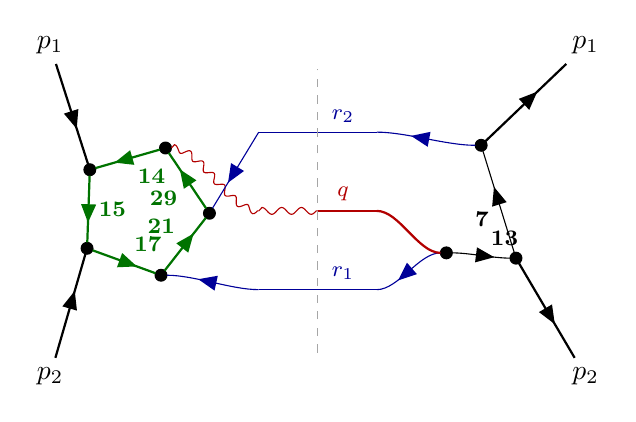
\begin{tikzpicture}
\begin{feynman}
\vertex (Lp1) at (-3.400,2.100) {$p_1$};
\vertex (Lp2) at (-3.400,-2.100) {$p_2$};
\vertex (Lcr1) at (-0.750,-1.000);
\vertex (Lcr2) at (-0.750,1.000);
\vertex (Lcq) at (-0.750,0.000);
\vertex (Mq) at (0,0.000);
\vertex[dot] (Lv0) at (-1.934,0.799) {};
\vertex[dot] (Lv1) at (-2.895,0.523) {};
\vertex[dot] (Lv2) at (-2.930,-0.475) {};
\vertex[dot] (Lv3) at (-1.991,-0.817) {};
\vertex[dot] (Lv4) at (-1.376,-0.030) {};
\vertex (Rp1) at (3.400,2.100) {$p_1$};
\vertex (Rp2) at (3.400,-2.100) {$p_2$};
\vertex (Rcr1) at (0.750,-1.000);
\vertex (Rcr2) at (0.750,1.000);
\vertex (Rcq) at (0.750,0.000);
\vertex[dot] (R7) at (2.075,0.833) {};
\vertex[dot] (R13) at (2.517,-0.600) {};
\vertex[dot] (Rroot) at (1.633,-0.533) {};
\diagram* {
(Lv0) -- [plain, thick, green!45!black, with arrow=0.55, edge label={\footnotesize\bfseries 14}] (Lv1),
(Lv1) -- [plain, thick, green!45!black, with arrow=0.55, edge label={\footnotesize\bfseries 15}] (Lv2),
(Lv2) -- [plain, thick, green!45!black, with arrow=0.55, edge label={\footnotesize\bfseries 17}] (Lv3),
(Lv3) -- [plain, thick, green!45!black, with arrow=0.55, edge label={\footnotesize\bfseries 21}] (Lv4),
(Lv4) -- [plain, thick, green!45!black, with arrow=0.55, edge label={\footnotesize\bfseries 29}] (Lv0),
(Lcq) -- [boson, red!70!black, out=180, in=0, looseness=0.75] (Lv0),
(Lp1) -- [plain, thick, with arrow=0.55] (Lv1),
(Lp2) -- [plain, thick, with arrow=0.55] (Lv2),
(Lcr1) -- [plain, blue!60!black, out=180, in=0, looseness=0.75, with arrow=0.55] (Lv3),
(Lcr2) -- [plain, blue!60!black, with arrow=0.55] (Lv4),
(R13) -- [plain, with arrow=0.55, edge label={\footnotesize\bfseries 7}] (R7),
(Rroot) -- [plain, out=0, in=180, looseness=0.75, with arrow=0.55, edge label={\footnotesize\bfseries 13}] (R13),
(R7) -- [plain, thick, with arrow=0.55] (Rp1),
(R13) -- [plain, thick, with arrow=0.55] (Rp2),
(Rroot) -- [plain, blue!60!black, out=180, in=0, looseness=0.75, with arrow=0.55] (Rcr1),
(R7) -- [plain, blue!60!black, out=180, in=0, looseness=0.75, with arrow=0.55] (Rcr2),
(Rroot) -- [plain, red!70!black, double, double distance=1.2pt, thick, out=180, in=0, looseness=0.75] (Rcq),
(Rcr1) -- [plain, blue!60!black] (Lcr1),
(Rcr2) -- [plain, blue!60!black] (Lcr2),
(Rcq) -- [plain, red!70!black, double, double distance=1.2pt, thick] (Mq) -- [boson, red!70!black] (Lcq),
};
\end{feynman}
\draw[dashed, gray!70] (0,-1.80) -- (0,1.80);
\node[font=\footnotesize, blue!60!black, above] at (0.32,-1.00) {$r_1$};
\node[font=\footnotesize, blue!60!black, above] at (0.32,1.00) {$r_2$};
\node[font=\footnotesize, red!70!black, above] at (0.32,0.00) {$q$};
\end{tikzpicture}}\\[2mm]\textbf{topo33} (RR family 28, pentagon q-p1-p2-r1-r2)\\[2pt]{\footnotesize\begin{tabular}{@{}r@{\ \ }l@{\ \ }l@{}}\textbf{14} & $(k_1)^2$ & loop\\
\textbf{15} & $(k_1+p_1)^2$ & loop\\
\textbf{17} & $(k_1+p_1+p_2)^2$ & loop\\
\textbf{21} & $(k_1+p_1+p_2+r_1)^2$ & loop\\
\textbf{29} & $(k_1+p_1+p_2+r_1+r_2)^2$ & loop\\
\textbf{7} & $(p_1+r_2)^2$ & conjugate\\
\textbf{13} & $(p_1+p_2+r_2)^2$ & conjugate\\
\textbf{10} & $(p_2+r_1+r_2)^2$ & \textcolor{red}{irreducible numerator}\\\end{tabular}}\end{minipage}\hfill%
\begin{minipage}[t]{0.48\textwidth}\centering\resizebox{0.9\linewidth}{!}{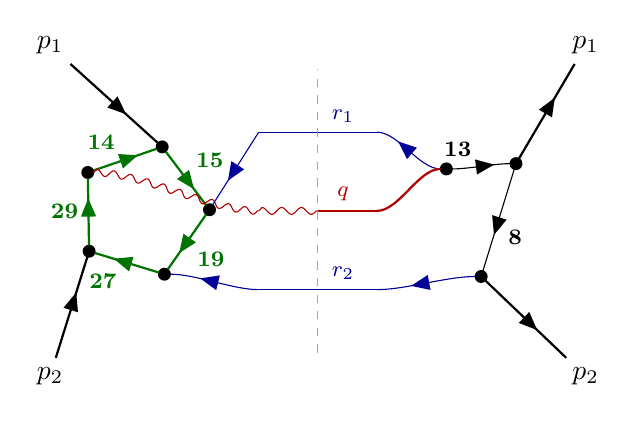
\begin{tikzpicture}
\begin{feynman}
\vertex (Lp1) at (-3.400,2.100) {$p_1$};
\vertex (Lp2) at (-3.400,-2.100) {$p_2$};
\vertex (Lcr1) at (-0.750,1.000);
\vertex (Lcr2) at (-0.750,-1.000);
\vertex (Lcq) at (-0.750,0.000);
\vertex (Mq) at (0,0.000);
\vertex[dot] (Lv0) at (-2.921,0.488) {};
\vertex[dot] (Lv1) at (-1.976,0.813) {};
\vertex[dot] (Lv2) at (-1.375,0.015) {};
\vertex[dot] (Lv3) at (-1.948,-0.804) {};
\vertex[dot] (Lv4) at (-2.904,-0.512) {};
\vertex (Rp1) at (3.400,2.100) {$p_1$};
\vertex (Rp2) at (3.400,-2.100) {$p_2$};
\vertex (Rcr1) at (0.750,1.000);
\vertex (Rcr2) at (0.750,-1.000);
\vertex (Rcq) at (0.750,0.000);
\vertex[dot] (R8) at (2.075,-0.833) {};
\vertex[dot] (R13) at (2.517,0.600) {};
\vertex[dot] (Rroot) at (1.633,0.533) {};
\diagram* {
(Lv0) -- [plain, thick, green!45!black, with arrow=0.55, edge label={\footnotesize\bfseries 14}] (Lv1),
(Lv1) -- [plain, thick, green!45!black, with arrow=0.55, edge label={\footnotesize\bfseries 15}] (Lv2),
(Lv2) -- [plain, thick, green!45!black, with arrow=0.55, edge label={\footnotesize\bfseries 19}] (Lv3),
(Lv3) -- [plain, thick, green!45!black, with arrow=0.55, edge label={\footnotesize\bfseries 27}] (Lv4),
(Lv4) -- [plain, thick, green!45!black, with arrow=0.55, edge label={\footnotesize\bfseries 29}] (Lv0),
(Lcq) -- [boson, red!70!black, out=180, in=0, looseness=0.75] (Lv0),
(Lp1) -- [plain, thick, with arrow=0.55] (Lv1),
(Lcr1) -- [plain, blue!60!black, with arrow=0.55] (Lv2),
(Lcr2) -- [plain, blue!60!black, out=180, in=0, looseness=0.75, with arrow=0.55] (Lv3),
(Lp2) -- [plain, thick, with arrow=0.55] (Lv4),
(R13) -- [plain, with arrow=0.55, edge label={\footnotesize\bfseries 8}] (R8),
(Rroot) -- [plain, out=0, in=180, looseness=0.75, with arrow=0.55, edge label={\footnotesize\bfseries 13}] (R13),
(R13) -- [plain, thick, with arrow=0.55] (Rp1),
(R8) -- [plain, thick, with arrow=0.55] (Rp2),
(Rroot) -- [plain, blue!60!black, out=180, in=0, looseness=0.75, with arrow=0.55] (Rcr1),
(R8) -- [plain, blue!60!black, out=180, in=0, looseness=0.75, with arrow=0.55] (Rcr2),
(Rroot) -- [plain, red!70!black, double, double distance=1.2pt, thick, out=180, in=0, looseness=0.75] (Rcq),
(Rcr1) -- [plain, blue!60!black] (Lcr1),
(Rcr2) -- [plain, blue!60!black] (Lcr2),
(Rcq) -- [plain, red!70!black, double, double distance=1.2pt, thick] (Mq) -- [boson, red!70!black] (Lcq),
};
\end{feynman}
\draw[dashed, gray!70] (0,-1.80) -- (0,1.80);
\node[font=\footnotesize, blue!60!black, above] at (0.32,1.00) {$r_1$};
\node[font=\footnotesize, blue!60!black, above] at (0.32,-1.00) {$r_2$};
\node[font=\footnotesize, red!70!black, above] at (0.32,0.00) {$q$};
\end{tikzpicture}}\\[2mm]\textbf{topo34} (RR family 34, pentagon q-p1-r1-r2-p2)\\[2pt]{\footnotesize\begin{tabular}{@{}r@{\ \ }l@{\ \ }l@{}}\textbf{14} & $(k_1)^2$ & loop\\
\textbf{15} & $(k_1+p_1)^2$ & loop\\
\textbf{19} & $(k_1+p_1+r_1)^2$ & loop\\
\textbf{27} & $(k_1+p_1+r_1+r_2)^2$ & loop\\
\textbf{29} & $(k_1+p_1+p_2+r_1+r_2)^2$ & loop\\
\textbf{8} & $(p_2+r_2)^2$ & conjugate\\
\textbf{13} & $(p_1+p_2+r_2)^2$ & conjugate\\
\textbf{9} & $(p_1+r_1+r_2)^2$ & \textcolor{red}{irreducible numerator}\\\end{tabular}}\end{minipage}

\bigskip

\begin{minipage}[t]{0.48\textwidth}\centering\resizebox{0.9\linewidth}{!}{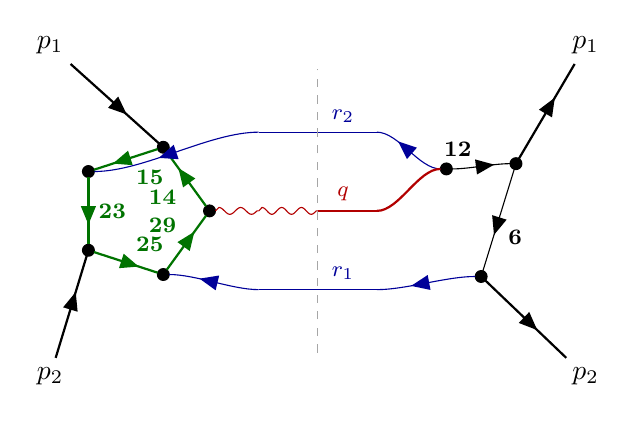
\begin{tikzpicture}
\begin{feynman}
\vertex (Lp1) at (-3.400,2.100) {$p_1$};
\vertex (Lp2) at (-3.400,-2.100) {$p_2$};
\vertex (Lcr1) at (-0.750,-1.000);
\vertex (Lcr2) at (-0.750,1.000);
\vertex (Lcq) at (-0.750,0.000);
\vertex (Mq) at (0,0.000);
\vertex[dot] (Lv0) at (-1.375,0.000) {};
\vertex[dot] (Lv1) at (-1.962,0.808) {};
\vertex[dot] (Lv2) at (-2.913,0.500) {};
\vertex[dot] (Lv3) at (-2.913,-0.500) {};
\vertex[dot] (Lv4) at (-1.962,-0.808) {};
\vertex (Rp1) at (3.400,2.100) {$p_1$};
\vertex (Rp2) at (3.400,-2.100) {$p_2$};
\vertex (Rcr1) at (0.750,-1.000);
\vertex (Rcr2) at (0.750,1.000);
\vertex (Rcq) at (0.750,0.000);
\vertex[dot] (R6) at (2.075,-0.833) {};
\vertex[dot] (R12) at (2.517,0.600) {};
\vertex[dot] (Rroot) at (1.633,0.533) {};
\diagram* {
(Lv0) -- [plain, thick, green!45!black, with arrow=0.55, edge label={\footnotesize\bfseries 14}] (Lv1),
(Lv1) -- [plain, thick, green!45!black, with arrow=0.55, edge label={\footnotesize\bfseries 15}] (Lv2),
(Lv2) -- [plain, thick, green!45!black, with arrow=0.55, edge label={\footnotesize\bfseries 23}] (Lv3),
(Lv3) -- [plain, thick, green!45!black, with arrow=0.55, edge label={\footnotesize\bfseries 25}] (Lv4),
(Lv4) -- [plain, thick, green!45!black, with arrow=0.55, edge label={\footnotesize\bfseries 29}] (Lv0),
(Lcq) -- [boson, red!70!black] (Lv0),
(Lp1) -- [plain, thick, with arrow=0.55] (Lv1),
(Lcr2) -- [plain, blue!60!black, out=180, in=0, looseness=0.75, with arrow=0.55] (Lv2),
(Lp2) -- [plain, thick, with arrow=0.55] (Lv3),
(Lcr1) -- [plain, blue!60!black, out=180, in=0, looseness=0.75, with arrow=0.55] (Lv4),
(R12) -- [plain, with arrow=0.55, edge label={\footnotesize\bfseries 6}] (R6),
(Rroot) -- [plain, out=0, in=180, looseness=0.75, with arrow=0.55, edge label={\footnotesize\bfseries 12}] (R12),
(R12) -- [plain, thick, with arrow=0.55] (Rp1),
(R6) -- [plain, thick, with arrow=0.55] (Rp2),
(R6) -- [plain, blue!60!black, out=180, in=0, looseness=0.75, with arrow=0.55] (Rcr1),
(Rroot) -- [plain, blue!60!black, out=180, in=0, looseness=0.75, with arrow=0.55] (Rcr2),
(Rroot) -- [plain, red!70!black, double, double distance=1.2pt, thick, out=180, in=0, looseness=0.75] (Rcq),
(Rcr1) -- [plain, blue!60!black] (Lcr1),
(Rcr2) -- [plain, blue!60!black] (Lcr2),
(Rcq) -- [plain, red!70!black, double, double distance=1.2pt, thick] (Mq) -- [boson, red!70!black] (Lcq),
};
\end{feynman}
\draw[dashed, gray!70] (0,-1.80) -- (0,1.80);
\node[font=\footnotesize, blue!60!black, above] at (0.32,-1.00) {$r_1$};
\node[font=\footnotesize, blue!60!black, above] at (0.32,1.00) {$r_2$};
\node[font=\footnotesize, red!70!black, above] at (0.32,0.00) {$q$};
\end{tikzpicture}}\\[2mm]\textbf{topo35} (RR family 24, pentagon q-p1-r2-p2-r1)\\[2pt]{\footnotesize\begin{tabular}{@{}r@{\ \ }l@{\ \ }l@{}}\textbf{14} & $(k_1)^2$ & loop\\
\textbf{15} & $(k_1+p_1)^2$ & loop\\
\textbf{23} & $(k_1+p_1+r_2)^2$ & loop\\
\textbf{25} & $(k_1+p_1+p_2+r_2)^2$ & loop\\
\textbf{29} & $(k_1+p_1+p_2+r_1+r_2)^2$ & loop\\
\textbf{6} & $(p_2+r_1)^2$ & conjugate\\
\textbf{12} & $(p_1+p_2+r_1)^2$ & conjugate\\
\textbf{13} & $(p_1+p_2+r_2)^2$ & \textcolor{red}{irreducible numerator}\\\end{tabular}}\end{minipage}\hfill%
\begin{minipage}[t]{0.48\textwidth}\centering\resizebox{0.9\linewidth}{!}{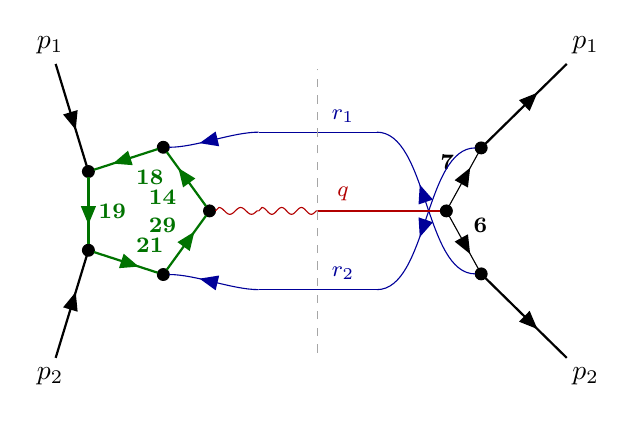
\begin{tikzpicture}
\begin{feynman}
\vertex (Lp1) at (-3.400,2.100) {$p_1$};
\vertex (Lp2) at (-3.400,-2.100) {$p_2$};
\vertex (Lcr1) at (-0.750,1.000);
\vertex (Lcr2) at (-0.750,-1.000);
\vertex (Lcq) at (-0.750,0.000);
\vertex (Mq) at (0,0.000);
\vertex[dot] (Lv0) at (-1.375,0.000) {};
\vertex[dot] (Lv1) at (-1.962,0.808) {};
\vertex[dot] (Lv2) at (-2.913,0.500) {};
\vertex[dot] (Lv3) at (-2.913,-0.500) {};
\vertex[dot] (Lv4) at (-1.962,-0.808) {};
\vertex (Rp1) at (3.400,2.100) {$p_1$};
\vertex (Rp2) at (3.400,-2.100) {$p_2$};
\vertex (Rcr1) at (0.750,1.000);
\vertex (Rcr2) at (0.750,-1.000);
\vertex (Rcq) at (0.750,0.000);
\vertex[dot] (R6) at (2.075,-0.800) {};
\vertex[dot] (Rroot) at (1.633,-0.000) {};
\vertex[dot] (R7) at (2.075,0.800) {};
\diagram* {
(Lv0) -- [plain, thick, green!45!black, with arrow=0.55, edge label={\footnotesize\bfseries 14}] (Lv1),
(Lv1) -- [plain, thick, green!45!black, with arrow=0.55, edge label={\footnotesize\bfseries 18}] (Lv2),
(Lv2) -- [plain, thick, green!45!black, with arrow=0.55, edge label={\footnotesize\bfseries 19}] (Lv3),
(Lv3) -- [plain, thick, green!45!black, with arrow=0.55, edge label={\footnotesize\bfseries 21}] (Lv4),
(Lv4) -- [plain, thick, green!45!black, with arrow=0.55, edge label={\footnotesize\bfseries 29}] (Lv0),
(Lcq) -- [boson, red!70!black] (Lv0),
(Lcr1) -- [plain, blue!60!black, out=180, in=0, looseness=0.75, with arrow=0.55] (Lv1),
(Lp1) -- [plain, thick, with arrow=0.55] (Lv2),
(Lp2) -- [plain, thick, with arrow=0.55] (Lv3),
(Lcr2) -- [plain, blue!60!black, out=180, in=0, looseness=0.75, with arrow=0.55] (Lv4),
(Rroot) -- [plain, with arrow=0.55, edge label={\footnotesize\bfseries 6}] (R6),
(Rroot) -- [plain, with arrow=0.55, edge label={\footnotesize\bfseries 7}] (R7),
(R7) -- [plain, thick, with arrow=0.55] (Rp1),
(R6) -- [plain, thick, with arrow=0.55] (Rp2),
(R6) -- [plain, blue!60!black, out=180, in=0, looseness=0.75, with arrow=0.55] (Rcr1),
(R7) -- [plain, blue!60!black, out=180, in=0, looseness=0.75, with arrow=0.55] (Rcr2),
(Rroot) -- [plain, red!70!black, double, double distance=1.2pt, thick] (Rcq),
(Rcr1) -- [plain, blue!60!black] (Lcr1),
(Rcr2) -- [plain, blue!60!black] (Lcr2),
(Rcq) -- [plain, red!70!black, double, double distance=1.2pt, thick] (Mq) -- [boson, red!70!black] (Lcq),
};
\end{feynman}
\draw[dashed, gray!70] (0,-1.80) -- (0,1.80);
\node[font=\footnotesize, blue!60!black, above] at (0.32,1.00) {$r_1$};
\node[font=\footnotesize, blue!60!black, above] at (0.32,-1.00) {$r_2$};
\node[font=\footnotesize, red!70!black, above] at (0.32,0.00) {$q$};
\end{tikzpicture}}\\[2mm]\textbf{topo36} (RR family 1, pentagon q-r1-p1-p2-r2)\\[2pt]{\footnotesize\begin{tabular}{@{}r@{\ \ }l@{\ \ }l@{}}\textbf{14} & $(k_1)^2$ & loop\\
\textbf{18} & $(k_1+r_1)^2$ & loop\\
\textbf{19} & $(k_1+p_1+r_1)^2$ & loop\\
\textbf{21} & $(k_1+p_1+p_2+r_1)^2$ & loop\\
\textbf{29} & $(k_1+p_1+p_2+r_1+r_2)^2$ & loop\\
\textbf{6} & $(p_2+r_1)^2$ & conjugate\\
\textbf{7} & $(p_1+r_2)^2$ & conjugate\\
\textbf{5} & $(p_1+r_1)^2$ & \textcolor{red}{irreducible numerator}\\\end{tabular}}\end{minipage}

\bigskip

\begin{minipage}[t]{0.48\textwidth}\centering\resizebox{0.9\linewidth}{!}{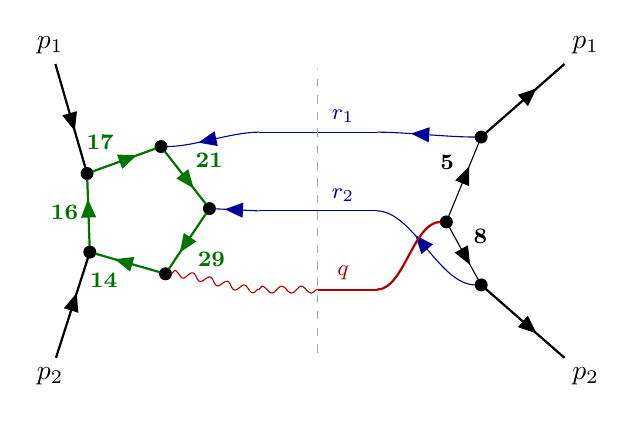
\begin{tikzpicture}
\begin{feynman}
\vertex (Lp1) at (-3.400,2.100) {$p_1$};
\vertex (Lp2) at (-3.400,-2.100) {$p_2$};
\vertex (Lcr1) at (-0.750,1.000);
\vertex (Lcr2) at (-0.750,0.000);
\vertex (Lcq) at (-0.750,-1.000);
\vertex (Mq) at (0,-1.000);
\vertex[dot] (Lv0) at (-1.934,-0.799) {};
\vertex[dot] (Lv1) at (-2.895,-0.523) {};
\vertex[dot] (Lv2) at (-2.930,0.475) {};
\vertex[dot] (Lv3) at (-1.991,0.817) {};
\vertex[dot] (Lv4) at (-1.376,0.030) {};
\vertex (Rp1) at (3.400,2.100) {$p_1$};
\vertex (Rp2) at (3.400,-2.100) {$p_2$};
\vertex (Rcr1) at (0.750,1.000);
\vertex (Rcr2) at (0.750,0.000);
\vertex (Rcq) at (0.750,-1.000);
\vertex[dot] (R5) at (2.075,0.938) {};
\vertex[dot] (Rroot) at (1.633,-0.140) {};
\vertex[dot] (R8) at (2.075,-0.940) {};
\diagram* {
(Lv0) -- [plain, thick, green!45!black, with arrow=0.55, edge label={\footnotesize\bfseries 14}] (Lv1),
(Lv1) -- [plain, thick, green!45!black, with arrow=0.55, edge label={\footnotesize\bfseries 16}] (Lv2),
(Lv2) -- [plain, thick, green!45!black, with arrow=0.55, edge label={\footnotesize\bfseries 17}] (Lv3),
(Lv3) -- [plain, thick, green!45!black, with arrow=0.55, edge label={\footnotesize\bfseries 21}] (Lv4),
(Lv4) -- [plain, thick, green!45!black, with arrow=0.55, edge label={\footnotesize\bfseries 29}] (Lv0),
(Lcq) -- [boson, red!70!black, out=180, in=0, looseness=0.75] (Lv0),
(Lp2) -- [plain, thick, with arrow=0.55] (Lv1),
(Lp1) -- [plain, thick, with arrow=0.55] (Lv2),
(Lcr1) -- [plain, blue!60!black, out=180, in=0, looseness=0.75, with arrow=0.55] (Lv3),
(Lcr2) -- [plain, blue!60!black, with arrow=0.55] (Lv4),
(Rroot) -- [plain, with arrow=0.55, edge label={\footnotesize\bfseries 5}] (R5),
(Rroot) -- [plain, with arrow=0.55, edge label={\footnotesize\bfseries 8}] (R8),
(R5) -- [plain, thick, with arrow=0.55] (Rp1),
(R8) -- [plain, thick, with arrow=0.55] (Rp2),
(R5) -- [plain, blue!60!black, out=180, in=0, looseness=0.75, with arrow=0.55] (Rcr1),
(R8) -- [plain, blue!60!black, out=180, in=0, looseness=0.75, with arrow=0.55] (Rcr2),
(Rroot) -- [plain, red!70!black, double, double distance=1.2pt, thick, out=180, in=0, looseness=0.75] (Rcq),
(Rcr1) -- [plain, blue!60!black] (Lcr1),
(Rcr2) -- [plain, blue!60!black] (Lcr2),
(Rcq) -- [plain, red!70!black, double, double distance=1.2pt, thick] (Mq) -- [boson, red!70!black] (Lcq),
};
\end{feynman}
\draw[dashed, gray!70] (0,-1.80) -- (0,1.80);
\node[font=\footnotesize, blue!60!black, above] at (0.32,1.00) {$r_1$};
\node[font=\footnotesize, blue!60!black, above] at (0.32,0.00) {$r_2$};
\node[font=\footnotesize, red!70!black, above] at (0.32,-1.00) {$q$};
\end{tikzpicture}}\\[2mm]\textbf{topo37} (RR family 8, pentagon q-p2-p1-r1-r2)\\[2pt]{\footnotesize\begin{tabular}{@{}r@{\ \ }l@{\ \ }l@{}}\textbf{14} & $(k_1)^2$ & loop\\
\textbf{16} & $(k_1+p_2)^2$ & loop\\
\textbf{17} & $(k_1+p_1+p_2)^2$ & loop\\
\textbf{21} & $(k_1+p_1+p_2+r_1)^2$ & loop\\
\textbf{29} & $(k_1+p_1+p_2+r_1+r_2)^2$ & loop\\
\textbf{5} & $(p_1+r_1)^2$ & conjugate\\
\textbf{8} & $(p_2+r_2)^2$ & conjugate\\
\textbf{11} & $(r_1+r_2)^2$ & \textcolor{red}{irreducible numerator}\\\end{tabular}}\end{minipage}\hfill%
\begin{minipage}[t]{0.48\textwidth}\centering\resizebox{0.9\linewidth}{!}{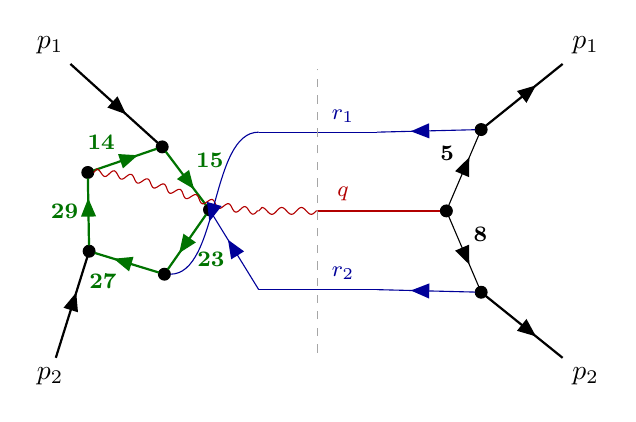
\begin{tikzpicture}
\begin{feynman}
\vertex (Lp1) at (-3.400,2.100) {$p_1$};
\vertex (Lp2) at (-3.400,-2.100) {$p_2$};
\vertex (Lcr1) at (-0.750,1.000);
\vertex (Lcr2) at (-0.750,-1.000);
\vertex (Lcq) at (-0.750,0.000);
\vertex (Mq) at (0,0.000);
\vertex[dot] (Lv0) at (-2.921,0.488) {};
\vertex[dot] (Lv1) at (-1.976,0.813) {};
\vertex[dot] (Lv2) at (-1.375,0.015) {};
\vertex[dot] (Lv3) at (-1.948,-0.804) {};
\vertex[dot] (Lv4) at (-2.904,-0.512) {};
\vertex (Rp1) at (3.400,2.100) {$p_1$};
\vertex (Rp2) at (3.400,-2.100) {$p_2$};
\vertex (Rcr1) at (0.750,1.000);
\vertex (Rcr2) at (0.750,-1.000);
\vertex (Rcq) at (0.750,0.000);
\vertex[dot] (R5) at (2.075,1.033) {};
\vertex[dot] (Rroot) at (1.633,0.000) {};
\vertex[dot] (R8) at (2.075,-1.033) {};
\diagram* {
(Lv0) -- [plain, thick, green!45!black, with arrow=0.55, edge label={\footnotesize\bfseries 14}] (Lv1),
(Lv1) -- [plain, thick, green!45!black, with arrow=0.55, edge label={\footnotesize\bfseries 15}] (Lv2),
(Lv2) -- [plain, thick, green!45!black, with arrow=0.55, edge label={\footnotesize\bfseries 23}] (Lv3),
(Lv3) -- [plain, thick, green!45!black, with arrow=0.55, edge label={\footnotesize\bfseries 27}] (Lv4),
(Lv4) -- [plain, thick, green!45!black, with arrow=0.55, edge label={\footnotesize\bfseries 29}] (Lv0),
(Lcq) -- [boson, red!70!black, out=180, in=0, looseness=0.75] (Lv0),
(Lp1) -- [plain, thick, with arrow=0.55] (Lv1),
(Lcr2) -- [plain, blue!60!black, with arrow=0.55] (Lv2),
(Lcr1) -- [plain, blue!60!black, out=180, in=0, looseness=0.75, with arrow=0.55] (Lv3),
(Lp2) -- [plain, thick, with arrow=0.55] (Lv4),
(Rroot) -- [plain, with arrow=0.55, edge label={\footnotesize\bfseries 5}] (R5),
(Rroot) -- [plain, with arrow=0.55, edge label={\footnotesize\bfseries 8}] (R8),
(R5) -- [plain, thick, with arrow=0.55] (Rp1),
(R8) -- [plain, thick, with arrow=0.55] (Rp2),
(R5) -- [plain, blue!60!black, with arrow=0.55] (Rcr1),
(R8) -- [plain, blue!60!black, with arrow=0.55] (Rcr2),
(Rroot) -- [plain, red!70!black, double, double distance=1.2pt, thick] (Rcq),
(Rcr1) -- [plain, blue!60!black] (Lcr1),
(Rcr2) -- [plain, blue!60!black] (Lcr2),
(Rcq) -- [plain, red!70!black, double, double distance=1.2pt, thick] (Mq) -- [boson, red!70!black] (Lcq),
};
\end{feynman}
\draw[dashed, gray!70] (0,-1.80) -- (0,1.80);
\node[font=\footnotesize, blue!60!black, above] at (0.32,1.00) {$r_1$};
\node[font=\footnotesize, blue!60!black, above] at (0.32,-1.00) {$r_2$};
\node[font=\footnotesize, red!70!black, above] at (0.32,0.00) {$q$};
\end{tikzpicture}}\\[2mm]\textbf{topo38} (RR family 2, pentagon q-p1-r2-r1-p2)\\[2pt]{\footnotesize\begin{tabular}{@{}r@{\ \ }l@{\ \ }l@{}}\textbf{14} & $(k_1)^2$ & loop\\
\textbf{15} & $(k_1+p_1)^2$ & loop\\
\textbf{23} & $(k_1+p_1+r_2)^2$ & loop\\
\textbf{27} & $(k_1+p_1+r_1+r_2)^2$ & loop\\
\textbf{29} & $(k_1+p_1+p_2+r_1+r_2)^2$ & loop\\
\textbf{5} & $(p_1+r_1)^2$ & conjugate\\
\textbf{8} & $(p_2+r_2)^2$ & conjugate\\
\textbf{6} & $(p_2+r_1)^2$ & \textcolor{red}{irreducible numerator}\\\end{tabular}}\end{minipage}

\bigskip

\begin{minipage}[t]{0.48\textwidth}\centering\resizebox{0.9\linewidth}{!}{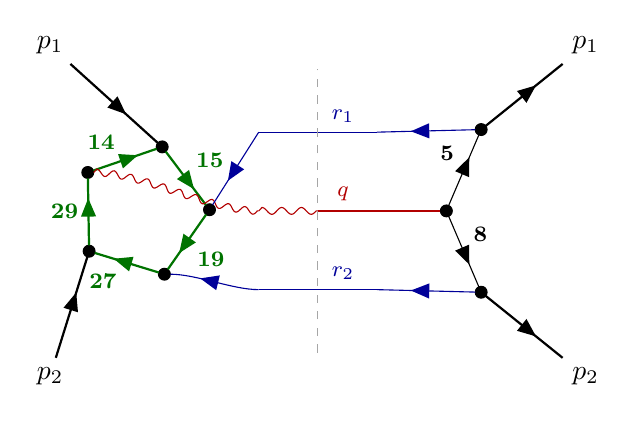
\begin{tikzpicture}
\begin{feynman}
\vertex (Lp1) at (-3.400,2.100) {$p_1$};
\vertex (Lp2) at (-3.400,-2.100) {$p_2$};
\vertex (Lcr1) at (-0.750,1.000);
\vertex (Lcr2) at (-0.750,-1.000);
\vertex (Lcq) at (-0.750,0.000);
\vertex (Mq) at (0,0.000);
\vertex[dot] (Lv0) at (-2.921,0.488) {};
\vertex[dot] (Lv1) at (-1.976,0.813) {};
\vertex[dot] (Lv2) at (-1.375,0.015) {};
\vertex[dot] (Lv3) at (-1.948,-0.804) {};
\vertex[dot] (Lv4) at (-2.904,-0.512) {};
\vertex (Rp1) at (3.400,2.100) {$p_1$};
\vertex (Rp2) at (3.400,-2.100) {$p_2$};
\vertex (Rcr1) at (0.750,1.000);
\vertex (Rcr2) at (0.750,-1.000);
\vertex (Rcq) at (0.750,0.000);
\vertex[dot] (R5) at (2.075,1.033) {};
\vertex[dot] (Rroot) at (1.633,0.000) {};
\vertex[dot] (R8) at (2.075,-1.033) {};
\diagram* {
(Lv0) -- [plain, thick, green!45!black, with arrow=0.55, edge label={\footnotesize\bfseries 14}] (Lv1),
(Lv1) -- [plain, thick, green!45!black, with arrow=0.55, edge label={\footnotesize\bfseries 15}] (Lv2),
(Lv2) -- [plain, thick, green!45!black, with arrow=0.55, edge label={\footnotesize\bfseries 19}] (Lv3),
(Lv3) -- [plain, thick, green!45!black, with arrow=0.55, edge label={\footnotesize\bfseries 27}] (Lv4),
(Lv4) -- [plain, thick, green!45!black, with arrow=0.55, edge label={\footnotesize\bfseries 29}] (Lv0),
(Lcq) -- [boson, red!70!black, out=180, in=0, looseness=0.75] (Lv0),
(Lp1) -- [plain, thick, with arrow=0.55] (Lv1),
(Lcr1) -- [plain, blue!60!black, with arrow=0.55] (Lv2),
(Lcr2) -- [plain, blue!60!black, out=180, in=0, looseness=0.75, with arrow=0.55] (Lv3),
(Lp2) -- [plain, thick, with arrow=0.55] (Lv4),
(Rroot) -- [plain, with arrow=0.55, edge label={\footnotesize\bfseries 5}] (R5),
(Rroot) -- [plain, with arrow=0.55, edge label={\footnotesize\bfseries 8}] (R8),
(R5) -- [plain, thick, with arrow=0.55] (Rp1),
(R8) -- [plain, thick, with arrow=0.55] (Rp2),
(R5) -- [plain, blue!60!black, with arrow=0.55] (Rcr1),
(R8) -- [plain, blue!60!black, with arrow=0.55] (Rcr2),
(Rroot) -- [plain, red!70!black, double, double distance=1.2pt, thick] (Rcq),
(Rcr1) -- [plain, blue!60!black] (Lcr1),
(Rcr2) -- [plain, blue!60!black] (Lcr2),
(Rcq) -- [plain, red!70!black, double, double distance=1.2pt, thick] (Mq) -- [boson, red!70!black] (Lcq),
};
\end{feynman}
\draw[dashed, gray!70] (0,-1.80) -- (0,1.80);
\node[font=\footnotesize, blue!60!black, above] at (0.32,1.00) {$r_1$};
\node[font=\footnotesize, blue!60!black, above] at (0.32,-1.00) {$r_2$};
\node[font=\footnotesize, red!70!black, above] at (0.32,0.00) {$q$};
\end{tikzpicture}}\\[2mm]\textbf{topo39} (RR family 6, pentagon q-p1-r1-r2-p2)\\[2pt]{\footnotesize\begin{tabular}{@{}r@{\ \ }l@{\ \ }l@{}}\textbf{14} & $(k_1)^2$ & loop\\
\textbf{15} & $(k_1+p_1)^2$ & loop\\
\textbf{19} & $(k_1+p_1+r_1)^2$ & loop\\
\textbf{27} & $(k_1+p_1+r_1+r_2)^2$ & loop\\
\textbf{29} & $(k_1+p_1+p_2+r_1+r_2)^2$ & loop\\
\textbf{5} & $(p_1+r_1)^2$ & conjugate\\
\textbf{8} & $(p_2+r_2)^2$ & conjugate\\
\textbf{9} & $(p_1+r_1+r_2)^2$ & \textcolor{red}{irreducible numerator}\\\end{tabular}}\end{minipage}\hfill%
\begin{minipage}[t]{0.48\textwidth}\centering\resizebox{0.9\linewidth}{!}{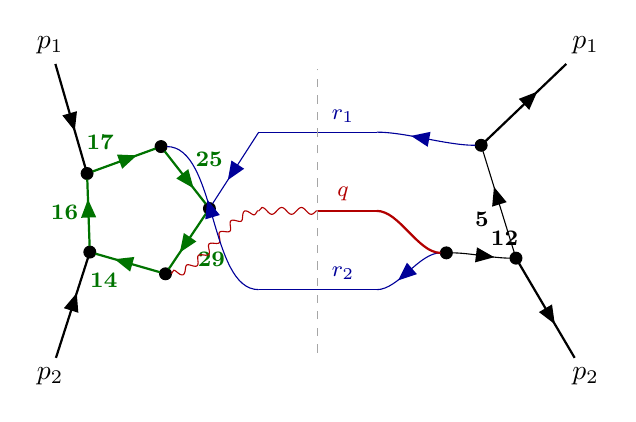
\begin{tikzpicture}
\begin{feynman}
\vertex (Lp1) at (-3.400,2.100) {$p_1$};
\vertex (Lp2) at (-3.400,-2.100) {$p_2$};
\vertex (Lcr1) at (-0.750,1.000);
\vertex (Lcr2) at (-0.750,-1.000);
\vertex (Lcq) at (-0.750,0.000);
\vertex (Mq) at (0,0.000);
\vertex[dot] (Lv0) at (-1.934,-0.799) {};
\vertex[dot] (Lv1) at (-2.895,-0.523) {};
\vertex[dot] (Lv2) at (-2.930,0.475) {};
\vertex[dot] (Lv3) at (-1.991,0.817) {};
\vertex[dot] (Lv4) at (-1.376,0.030) {};
\vertex (Rp1) at (3.400,2.100) {$p_1$};
\vertex (Rp2) at (3.400,-2.100) {$p_2$};
\vertex (Rcr1) at (0.750,1.000);
\vertex (Rcr2) at (0.750,-1.000);
\vertex (Rcq) at (0.750,0.000);
\vertex[dot] (R5) at (2.075,0.833) {};
\vertex[dot] (R12) at (2.517,-0.600) {};
\vertex[dot] (Rroot) at (1.633,-0.533) {};
\diagram* {
(Lv0) -- [plain, thick, green!45!black, with arrow=0.55, edge label={\footnotesize\bfseries 14}] (Lv1),
(Lv1) -- [plain, thick, green!45!black, with arrow=0.55, edge label={\footnotesize\bfseries 16}] (Lv2),
(Lv2) -- [plain, thick, green!45!black, with arrow=0.55, edge label={\footnotesize\bfseries 17}] (Lv3),
(Lv3) -- [plain, thick, green!45!black, with arrow=0.55, edge label={\footnotesize\bfseries 25}] (Lv4),
(Lv4) -- [plain, thick, green!45!black, with arrow=0.55, edge label={\footnotesize\bfseries 29}] (Lv0),
(Lcq) -- [boson, red!70!black, out=180, in=0, looseness=0.75] (Lv0),
(Lp2) -- [plain, thick, with arrow=0.55] (Lv1),
(Lp1) -- [plain, thick, with arrow=0.55] (Lv2),
(Lcr2) -- [plain, blue!60!black, out=180, in=0, looseness=0.75, with arrow=0.55] (Lv3),
(Lcr1) -- [plain, blue!60!black, with arrow=0.55] (Lv4),
(R12) -- [plain, with arrow=0.55, edge label={\footnotesize\bfseries 5}] (R5),
(Rroot) -- [plain, out=0, in=180, looseness=0.75, with arrow=0.55, edge label={\footnotesize\bfseries 12}] (R12),
(R5) -- [plain, thick, with arrow=0.55] (Rp1),
(R12) -- [plain, thick, with arrow=0.55] (Rp2),
(R5) -- [plain, blue!60!black, out=180, in=0, looseness=0.75, with arrow=0.55] (Rcr1),
(Rroot) -- [plain, blue!60!black, out=180, in=0, looseness=0.75, with arrow=0.55] (Rcr2),
(Rroot) -- [plain, red!70!black, double, double distance=1.2pt, thick, out=180, in=0, looseness=0.75] (Rcq),
(Rcr1) -- [plain, blue!60!black] (Lcr1),
(Rcr2) -- [plain, blue!60!black] (Lcr2),
(Rcq) -- [plain, red!70!black, double, double distance=1.2pt, thick] (Mq) -- [boson, red!70!black] (Lcq),
};
\end{feynman}
\draw[dashed, gray!70] (0,-1.80) -- (0,1.80);
\node[font=\footnotesize, blue!60!black, above] at (0.32,1.00) {$r_1$};
\node[font=\footnotesize, blue!60!black, above] at (0.32,-1.00) {$r_2$};
\node[font=\footnotesize, red!70!black, above] at (0.32,0.00) {$q$};
\end{tikzpicture}}\\[2mm]\textbf{topo40} (RR family 15, pentagon q-p2-p1-r2-r1)\\[2pt]{\footnotesize\begin{tabular}{@{}r@{\ \ }l@{\ \ }l@{}}\textbf{14} & $(k_1)^2$ & loop\\
\textbf{16} & $(k_1+p_2)^2$ & loop\\
\textbf{17} & $(k_1+p_1+p_2)^2$ & loop\\
\textbf{25} & $(k_1+p_1+p_2+r_2)^2$ & loop\\
\textbf{29} & $(k_1+p_1+p_2+r_1+r_2)^2$ & loop\\
\textbf{5} & $(p_1+r_1)^2$ & conjugate\\
\textbf{12} & $(p_1+p_2+r_1)^2$ & conjugate\\
\textbf{7} & $(p_1+r_2)^2$ & \textcolor{red}{irreducible numerator}\\\end{tabular}}\end{minipage}

\bigskip

\begin{minipage}[t]{0.48\textwidth}\centering\resizebox{0.9\linewidth}{!}{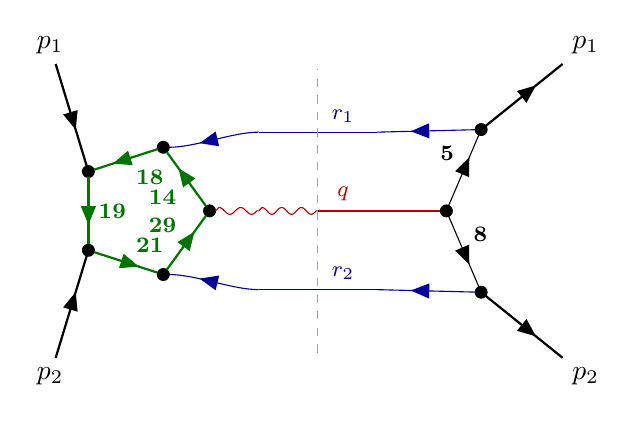
\begin{tikzpicture}
\begin{feynman}
\vertex (Lp1) at (-3.400,2.100) {$p_1$};
\vertex (Lp2) at (-3.400,-2.100) {$p_2$};
\vertex (Lcr1) at (-0.750,1.000);
\vertex (Lcr2) at (-0.750,-1.000);
\vertex (Lcq) at (-0.750,0.000);
\vertex (Mq) at (0,0.000);
\vertex[dot] (Lv0) at (-1.375,0.000) {};
\vertex[dot] (Lv1) at (-1.962,0.808) {};
\vertex[dot] (Lv2) at (-2.913,0.500) {};
\vertex[dot] (Lv3) at (-2.913,-0.500) {};
\vertex[dot] (Lv4) at (-1.962,-0.808) {};
\vertex (Rp1) at (3.400,2.100) {$p_1$};
\vertex (Rp2) at (3.400,-2.100) {$p_2$};
\vertex (Rcr1) at (0.750,1.000);
\vertex (Rcr2) at (0.750,-1.000);
\vertex (Rcq) at (0.750,0.000);
\vertex[dot] (R5) at (2.075,1.033) {};
\vertex[dot] (Rroot) at (1.633,0.000) {};
\vertex[dot] (R8) at (2.075,-1.033) {};
\diagram* {
(Lv0) -- [plain, thick, green!45!black, with arrow=0.55, edge label={\footnotesize\bfseries 14}] (Lv1),
(Lv1) -- [plain, thick, green!45!black, with arrow=0.55, edge label={\footnotesize\bfseries 18}] (Lv2),
(Lv2) -- [plain, thick, green!45!black, with arrow=0.55, edge label={\footnotesize\bfseries 19}] (Lv3),
(Lv3) -- [plain, thick, green!45!black, with arrow=0.55, edge label={\footnotesize\bfseries 21}] (Lv4),
(Lv4) -- [plain, thick, green!45!black, with arrow=0.55, edge label={\footnotesize\bfseries 29}] (Lv0),
(Lcq) -- [boson, red!70!black] (Lv0),
(Lcr1) -- [plain, blue!60!black, out=180, in=0, looseness=0.75, with arrow=0.55] (Lv1),
(Lp1) -- [plain, thick, with arrow=0.55] (Lv2),
(Lp2) -- [plain, thick, with arrow=0.55] (Lv3),
(Lcr2) -- [plain, blue!60!black, out=180, in=0, looseness=0.75, with arrow=0.55] (Lv4),
(Rroot) -- [plain, with arrow=0.55, edge label={\footnotesize\bfseries 5}] (R5),
(Rroot) -- [plain, with arrow=0.55, edge label={\footnotesize\bfseries 8}] (R8),
(R5) -- [plain, thick, with arrow=0.55] (Rp1),
(R8) -- [plain, thick, with arrow=0.55] (Rp2),
(R5) -- [plain, blue!60!black, with arrow=0.55] (Rcr1),
(R8) -- [plain, blue!60!black, with arrow=0.55] (Rcr2),
(Rroot) -- [plain, red!70!black, double, double distance=1.2pt, thick] (Rcq),
(Rcr1) -- [plain, blue!60!black] (Lcr1),
(Rcr2) -- [plain, blue!60!black] (Lcr2),
(Rcq) -- [plain, red!70!black, double, double distance=1.2pt, thick] (Mq) -- [boson, red!70!black] (Lcq),
};
\end{feynman}
\draw[dashed, gray!70] (0,-1.80) -- (0,1.80);
\node[font=\footnotesize, blue!60!black, above] at (0.32,1.00) {$r_1$};
\node[font=\footnotesize, blue!60!black, above] at (0.32,-1.00) {$r_2$};
\node[font=\footnotesize, red!70!black, above] at (0.32,0.00) {$q$};
\end{tikzpicture}}\\[2mm]\textbf{topo41} (RR family 18, pentagon q-r1-p1-p2-r2)\\[2pt]{\footnotesize\begin{tabular}{@{}r@{\ \ }l@{\ \ }l@{}}\textbf{14} & $(k_1)^2$ & loop\\
\textbf{18} & $(k_1+r_1)^2$ & loop\\
\textbf{19} & $(k_1+p_1+r_1)^2$ & loop\\
\textbf{21} & $(k_1+p_1+p_2+r_1)^2$ & loop\\
\textbf{29} & $(k_1+p_1+p_2+r_1+r_2)^2$ & loop\\
\textbf{5} & $(p_1+r_1)^2$ & conjugate\\
\textbf{8} & $(p_2+r_2)^2$ & conjugate\\
\textbf{13} & $(p_1+p_2+r_2)^2$ & \textcolor{red}{irreducible numerator}\\\end{tabular}}\end{minipage}\hfill%
\begin{minipage}[t]{0.48\textwidth}\centering\resizebox{0.9\linewidth}{!}{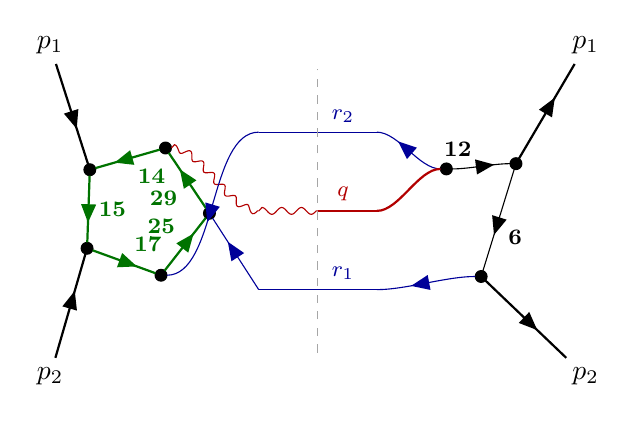
\begin{tikzpicture}
\begin{feynman}
\vertex (Lp1) at (-3.400,2.100) {$p_1$};
\vertex (Lp2) at (-3.400,-2.100) {$p_2$};
\vertex (Lcr1) at (-0.750,-1.000);
\vertex (Lcr2) at (-0.750,1.000);
\vertex (Lcq) at (-0.750,0.000);
\vertex (Mq) at (0,0.000);
\vertex[dot] (Lv0) at (-1.934,0.799) {};
\vertex[dot] (Lv1) at (-2.895,0.523) {};
\vertex[dot] (Lv2) at (-2.930,-0.475) {};
\vertex[dot] (Lv3) at (-1.991,-0.817) {};
\vertex[dot] (Lv4) at (-1.376,-0.030) {};
\vertex (Rp1) at (3.400,2.100) {$p_1$};
\vertex (Rp2) at (3.400,-2.100) {$p_2$};
\vertex (Rcr1) at (0.750,-1.000);
\vertex (Rcr2) at (0.750,1.000);
\vertex (Rcq) at (0.750,0.000);
\vertex[dot] (R6) at (2.075,-0.833) {};
\vertex[dot] (R12) at (2.517,0.600) {};
\vertex[dot] (Rroot) at (1.633,0.533) {};
\diagram* {
(Lv0) -- [plain, thick, green!45!black, with arrow=0.55, edge label={\footnotesize\bfseries 14}] (Lv1),
(Lv1) -- [plain, thick, green!45!black, with arrow=0.55, edge label={\footnotesize\bfseries 15}] (Lv2),
(Lv2) -- [plain, thick, green!45!black, with arrow=0.55, edge label={\footnotesize\bfseries 17}] (Lv3),
(Lv3) -- [plain, thick, green!45!black, with arrow=0.55, edge label={\footnotesize\bfseries 25}] (Lv4),
(Lv4) -- [plain, thick, green!45!black, with arrow=0.55, edge label={\footnotesize\bfseries 29}] (Lv0),
(Lcq) -- [boson, red!70!black, out=180, in=0, looseness=0.75] (Lv0),
(Lp1) -- [plain, thick, with arrow=0.55] (Lv1),
(Lp2) -- [plain, thick, with arrow=0.55] (Lv2),
(Lcr2) -- [plain, blue!60!black, out=180, in=0, looseness=0.75, with arrow=0.55] (Lv3),
(Lcr1) -- [plain, blue!60!black, with arrow=0.55] (Lv4),
(R12) -- [plain, with arrow=0.55, edge label={\footnotesize\bfseries 6}] (R6),
(Rroot) -- [plain, out=0, in=180, looseness=0.75, with arrow=0.55, edge label={\footnotesize\bfseries 12}] (R12),
(R12) -- [plain, thick, with arrow=0.55] (Rp1),
(R6) -- [plain, thick, with arrow=0.55] (Rp2),
(R6) -- [plain, blue!60!black, out=180, in=0, looseness=0.75, with arrow=0.55] (Rcr1),
(Rroot) -- [plain, blue!60!black, out=180, in=0, looseness=0.75, with arrow=0.55] (Rcr2),
(Rroot) -- [plain, red!70!black, double, double distance=1.2pt, thick, out=180, in=0, looseness=0.75] (Rcq),
(Rcr1) -- [plain, blue!60!black] (Lcr1),
(Rcr2) -- [plain, blue!60!black] (Lcr2),
(Rcq) -- [plain, red!70!black, double, double distance=1.2pt, thick] (Mq) -- [boson, red!70!black] (Lcq),
};
\end{feynman}
\draw[dashed, gray!70] (0,-1.80) -- (0,1.80);
\node[font=\footnotesize, blue!60!black, above] at (0.32,-1.00) {$r_1$};
\node[font=\footnotesize, blue!60!black, above] at (0.32,1.00) {$r_2$};
\node[font=\footnotesize, red!70!black, above] at (0.32,0.00) {$q$};
\end{tikzpicture}}\\[2mm]\textbf{topo42} (RR family 21, pentagon q-p1-p2-r2-r1)\\[2pt]{\footnotesize\begin{tabular}{@{}r@{\ \ }l@{\ \ }l@{}}\textbf{14} & $(k_1)^2$ & loop\\
\textbf{15} & $(k_1+p_1)^2$ & loop\\
\textbf{17} & $(k_1+p_1+p_2)^2$ & loop\\
\textbf{25} & $(k_1+p_1+p_2+r_2)^2$ & loop\\
\textbf{29} & $(k_1+p_1+p_2+r_1+r_2)^2$ & loop\\
\textbf{6} & $(p_2+r_1)^2$ & conjugate\\
\textbf{12} & $(p_1+p_2+r_1)^2$ & conjugate\\
\textbf{8} & $(p_2+r_2)^2$ & \textcolor{red}{irreducible numerator}\\\end{tabular}}\end{minipage}

\bigskip

\begin{minipage}[t]{0.48\textwidth}\centering\resizebox{0.9\linewidth}{!}{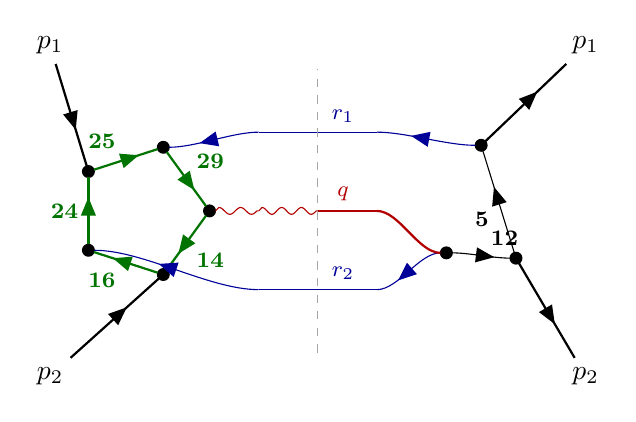
\begin{tikzpicture}
\begin{feynman}
\vertex (Lp1) at (-3.400,2.100) {$p_1$};
\vertex (Lp2) at (-3.400,-2.100) {$p_2$};
\vertex (Lcr1) at (-0.750,1.000);
\vertex (Lcr2) at (-0.750,-1.000);
\vertex (Lcq) at (-0.750,0.000);
\vertex (Mq) at (0,0.000);
\vertex[dot] (Lv0) at (-1.375,0.000) {};
\vertex[dot] (Lv1) at (-1.962,-0.808) {};
\vertex[dot] (Lv2) at (-2.913,-0.500) {};
\vertex[dot] (Lv3) at (-2.913,0.500) {};
\vertex[dot] (Lv4) at (-1.962,0.808) {};
\vertex (Rp1) at (3.400,2.100) {$p_1$};
\vertex (Rp2) at (3.400,-2.100) {$p_2$};
\vertex (Rcr1) at (0.750,1.000);
\vertex (Rcr2) at (0.750,-1.000);
\vertex (Rcq) at (0.750,0.000);
\vertex[dot] (R5) at (2.075,0.833) {};
\vertex[dot] (R12) at (2.517,-0.600) {};
\vertex[dot] (Rroot) at (1.633,-0.533) {};
\diagram* {
(Lv0) -- [plain, thick, green!45!black, with arrow=0.55, edge label={\footnotesize\bfseries 14}] (Lv1),
(Lv1) -- [plain, thick, green!45!black, with arrow=0.55, edge label={\footnotesize\bfseries 16}] (Lv2),
(Lv2) -- [plain, thick, green!45!black, with arrow=0.55, edge label={\footnotesize\bfseries 24}] (Lv3),
(Lv3) -- [plain, thick, green!45!black, with arrow=0.55, edge label={\footnotesize\bfseries 25}] (Lv4),
(Lv4) -- [plain, thick, green!45!black, with arrow=0.55, edge label={\footnotesize\bfseries 29}] (Lv0),
(Lcq) -- [boson, red!70!black] (Lv0),
(Lp2) -- [plain, thick, with arrow=0.55] (Lv1),
(Lcr2) -- [plain, blue!60!black, out=180, in=0, looseness=0.75, with arrow=0.55] (Lv2),
(Lp1) -- [plain, thick, with arrow=0.55] (Lv3),
(Lcr1) -- [plain, blue!60!black, out=180, in=0, looseness=0.75, with arrow=0.55] (Lv4),
(R12) -- [plain, with arrow=0.55, edge label={\footnotesize\bfseries 5}] (R5),
(Rroot) -- [plain, out=0, in=180, looseness=0.75, with arrow=0.55, edge label={\footnotesize\bfseries 12}] (R12),
(R5) -- [plain, thick, with arrow=0.55] (Rp1),
(R12) -- [plain, thick, with arrow=0.55] (Rp2),
(R5) -- [plain, blue!60!black, out=180, in=0, looseness=0.75, with arrow=0.55] (Rcr1),
(Rroot) -- [plain, blue!60!black, out=180, in=0, looseness=0.75, with arrow=0.55] (Rcr2),
(Rroot) -- [plain, red!70!black, double, double distance=1.2pt, thick, out=180, in=0, looseness=0.75] (Rcq),
(Rcr1) -- [plain, blue!60!black] (Lcr1),
(Rcr2) -- [plain, blue!60!black] (Lcr2),
(Rcq) -- [plain, red!70!black, double, double distance=1.2pt, thick] (Mq) -- [boson, red!70!black] (Lcq),
};
\end{feynman}
\draw[dashed, gray!70] (0,-1.80) -- (0,1.80);
\node[font=\footnotesize, blue!60!black, above] at (0.32,1.00) {$r_1$};
\node[font=\footnotesize, blue!60!black, above] at (0.32,-1.00) {$r_2$};
\node[font=\footnotesize, red!70!black, above] at (0.32,0.00) {$q$};
\end{tikzpicture}}\\[2mm]\textbf{topo43} (RR family 23, pentagon q-p2-r2-p1-r1)\\[2pt]{\footnotesize\begin{tabular}{@{}r@{\ \ }l@{\ \ }l@{}}\textbf{14} & $(k_1)^2$ & loop\\
\textbf{16} & $(k_1+p_2)^2$ & loop\\
\textbf{24} & $(k_1+p_2+r_2)^2$ & loop\\
\textbf{25} & $(k_1+p_1+p_2+r_2)^2$ & loop\\
\textbf{29} & $(k_1+p_1+p_2+r_1+r_2)^2$ & loop\\
\textbf{5} & $(p_1+r_1)^2$ & conjugate\\
\textbf{12} & $(p_1+p_2+r_1)^2$ & conjugate\\
\textbf{13} & $(p_1+p_2+r_2)^2$ & \textcolor{red}{irreducible numerator}\\\end{tabular}}\end{minipage}\hfill%
\begin{minipage}[t]{0.48\textwidth}\centering\resizebox{0.9\linewidth}{!}{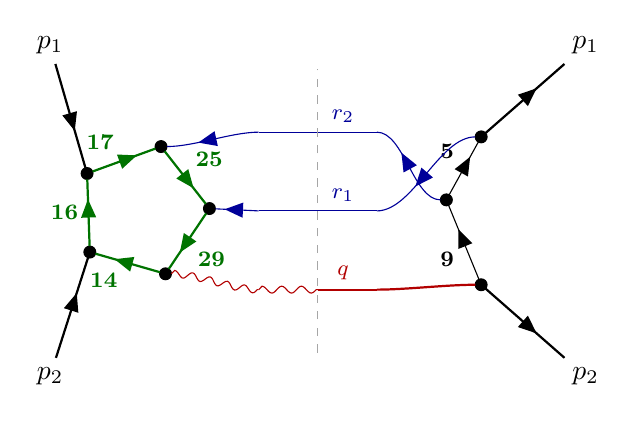
\begin{tikzpicture}
\begin{feynman}
\vertex (Lp1) at (-3.400,2.100) {$p_1$};
\vertex (Lp2) at (-3.400,-2.100) {$p_2$};
\vertex (Lcr1) at (-0.750,0.000);
\vertex (Lcr2) at (-0.750,1.000);
\vertex (Lcq) at (-0.750,-1.000);
\vertex (Mq) at (0,-1.000);
\vertex[dot] (Lv0) at (-1.934,-0.799) {};
\vertex[dot] (Lv1) at (-2.895,-0.523) {};
\vertex[dot] (Lv2) at (-2.930,0.475) {};
\vertex[dot] (Lv3) at (-1.991,0.817) {};
\vertex[dot] (Lv4) at (-1.376,0.030) {};
\vertex (Rp1) at (3.400,2.100) {$p_1$};
\vertex (Rp2) at (3.400,-2.100) {$p_2$};
\vertex (Rcr1) at (0.750,0.000);
\vertex (Rcr2) at (0.750,1.000);
\vertex (Rcq) at (0.750,-1.000);
\vertex[dot] (R5) at (2.075,0.940) {};
\vertex[dot] (R9) at (1.633,0.140) {};
\vertex[dot] (Rroot) at (2.075,-0.938) {};
\diagram* {
(Lv0) -- [plain, thick, green!45!black, with arrow=0.55, edge label={\footnotesize\bfseries 14}] (Lv1),
(Lv1) -- [plain, thick, green!45!black, with arrow=0.55, edge label={\footnotesize\bfseries 16}] (Lv2),
(Lv2) -- [plain, thick, green!45!black, with arrow=0.55, edge label={\footnotesize\bfseries 17}] (Lv3),
(Lv3) -- [plain, thick, green!45!black, with arrow=0.55, edge label={\footnotesize\bfseries 25}] (Lv4),
(Lv4) -- [plain, thick, green!45!black, with arrow=0.55, edge label={\footnotesize\bfseries 29}] (Lv0),
(Lcq) -- [boson, red!70!black, out=180, in=0, looseness=0.75] (Lv0),
(Lp2) -- [plain, thick, with arrow=0.55] (Lv1),
(Lp1) -- [plain, thick, with arrow=0.55] (Lv2),
(Lcr2) -- [plain, blue!60!black, out=180, in=0, looseness=0.75, with arrow=0.55] (Lv3),
(Lcr1) -- [plain, blue!60!black, with arrow=0.55] (Lv4),
(R9) -- [plain, with arrow=0.55, edge label={\footnotesize\bfseries 5}] (R5),
(Rroot) -- [plain, with arrow=0.55, edge label={\footnotesize\bfseries 9}] (R9),
(R5) -- [plain, thick, with arrow=0.55] (Rp1),
(Rroot) -- [plain, thick, with arrow=0.55] (Rp2),
(R5) -- [plain, blue!60!black, out=180, in=0, looseness=0.75, with arrow=0.55] (Rcr1),
(R9) -- [plain, blue!60!black, out=180, in=0, looseness=0.75, with arrow=0.55] (Rcr2),
(Rroot) -- [plain, red!70!black, double, double distance=1.2pt, thick, out=180, in=0, looseness=0.75] (Rcq),
(Rcr1) -- [plain, blue!60!black] (Lcr1),
(Rcr2) -- [plain, blue!60!black] (Lcr2),
(Rcq) -- [plain, red!70!black, double, double distance=1.2pt, thick] (Mq) -- [boson, red!70!black] (Lcq),
};
\end{feynman}
\draw[dashed, gray!70] (0,-1.80) -- (0,1.80);
\node[font=\footnotesize, blue!60!black, above] at (0.32,0.00) {$r_1$};
\node[font=\footnotesize, blue!60!black, above] at (0.32,1.00) {$r_2$};
\node[font=\footnotesize, red!70!black, above] at (0.32,-1.00) {$q$};
\end{tikzpicture}}\\[2mm]\textbf{topo44} (RR family 32, pentagon q-p2-p1-r2-r1)\\[2pt]{\footnotesize\begin{tabular}{@{}r@{\ \ }l@{\ \ }l@{}}\textbf{14} & $(k_1)^2$ & loop\\
\textbf{16} & $(k_1+p_2)^2$ & loop\\
\textbf{17} & $(k_1+p_1+p_2)^2$ & loop\\
\textbf{25} & $(k_1+p_1+p_2+r_2)^2$ & loop\\
\textbf{29} & $(k_1+p_1+p_2+r_1+r_2)^2$ & loop\\
\textbf{5} & $(p_1+r_1)^2$ & conjugate\\
\textbf{9} & $(p_1+r_1+r_2)^2$ & conjugate\\
\textbf{13} & $(p_1+p_2+r_2)^2$ & \textcolor{red}{irreducible numerator}\\\end{tabular}}\end{minipage}

\bigskip

\begin{minipage}[t]{0.48\textwidth}\centering\resizebox{0.9\linewidth}{!}{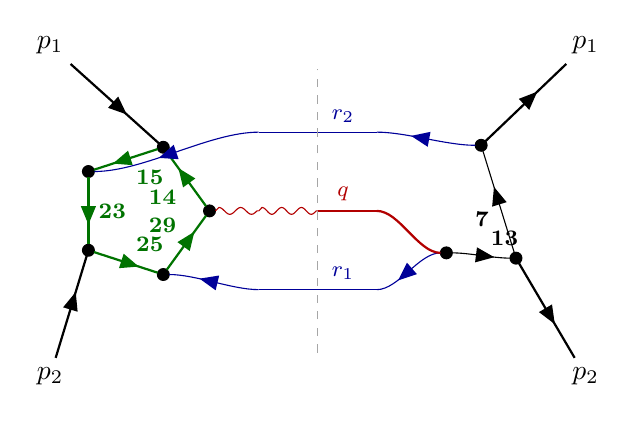
\begin{tikzpicture}
\begin{feynman}
\vertex (Lp1) at (-3.400,2.100) {$p_1$};
\vertex (Lp2) at (-3.400,-2.100) {$p_2$};
\vertex (Lcr1) at (-0.750,-1.000);
\vertex (Lcr2) at (-0.750,1.000);
\vertex (Lcq) at (-0.750,0.000);
\vertex (Mq) at (0,0.000);
\vertex[dot] (Lv0) at (-1.375,0.000) {};
\vertex[dot] (Lv1) at (-1.962,0.808) {};
\vertex[dot] (Lv2) at (-2.913,0.500) {};
\vertex[dot] (Lv3) at (-2.913,-0.500) {};
\vertex[dot] (Lv4) at (-1.962,-0.808) {};
\vertex (Rp1) at (3.400,2.100) {$p_1$};
\vertex (Rp2) at (3.400,-2.100) {$p_2$};
\vertex (Rcr1) at (0.750,-1.000);
\vertex (Rcr2) at (0.750,1.000);
\vertex (Rcq) at (0.750,0.000);
\vertex[dot] (R7) at (2.075,0.833) {};
\vertex[dot] (R13) at (2.517,-0.600) {};
\vertex[dot] (Rroot) at (1.633,-0.533) {};
\diagram* {
(Lv0) -- [plain, thick, green!45!black, with arrow=0.55, edge label={\footnotesize\bfseries 14}] (Lv1),
(Lv1) -- [plain, thick, green!45!black, with arrow=0.55, edge label={\footnotesize\bfseries 15}] (Lv2),
(Lv2) -- [plain, thick, green!45!black, with arrow=0.55, edge label={\footnotesize\bfseries 23}] (Lv3),
(Lv3) -- [plain, thick, green!45!black, with arrow=0.55, edge label={\footnotesize\bfseries 25}] (Lv4),
(Lv4) -- [plain, thick, green!45!black, with arrow=0.55, edge label={\footnotesize\bfseries 29}] (Lv0),
(Lcq) -- [boson, red!70!black] (Lv0),
(Lp1) -- [plain, thick, with arrow=0.55] (Lv1),
(Lcr2) -- [plain, blue!60!black, out=180, in=0, looseness=0.75, with arrow=0.55] (Lv2),
(Lp2) -- [plain, thick, with arrow=0.55] (Lv3),
(Lcr1) -- [plain, blue!60!black, out=180, in=0, looseness=0.75, with arrow=0.55] (Lv4),
(R13) -- [plain, with arrow=0.55, edge label={\footnotesize\bfseries 7}] (R7),
(Rroot) -- [plain, out=0, in=180, looseness=0.75, with arrow=0.55, edge label={\footnotesize\bfseries 13}] (R13),
(R7) -- [plain, thick, with arrow=0.55] (Rp1),
(R13) -- [plain, thick, with arrow=0.55] (Rp2),
(Rroot) -- [plain, blue!60!black, out=180, in=0, looseness=0.75, with arrow=0.55] (Rcr1),
(R7) -- [plain, blue!60!black, out=180, in=0, looseness=0.75, with arrow=0.55] (Rcr2),
(Rroot) -- [plain, red!70!black, double, double distance=1.2pt, thick, out=180, in=0, looseness=0.75] (Rcq),
(Rcr1) -- [plain, blue!60!black] (Lcr1),
(Rcr2) -- [plain, blue!60!black] (Lcr2),
(Rcq) -- [plain, red!70!black, double, double distance=1.2pt, thick] (Mq) -- [boson, red!70!black] (Lcq),
};
\end{feynman}
\draw[dashed, gray!70] (0,-1.80) -- (0,1.80);
\node[font=\footnotesize, blue!60!black, above] at (0.32,-1.00) {$r_1$};
\node[font=\footnotesize, blue!60!black, above] at (0.32,1.00) {$r_2$};
\node[font=\footnotesize, red!70!black, above] at (0.32,0.00) {$q$};
\end{tikzpicture}}\\[2mm]\textbf{topo45} (RR family 30, pentagon q-p1-r2-p2-r1)\\[2pt]{\footnotesize\begin{tabular}{@{}r@{\ \ }l@{\ \ }l@{}}\textbf{14} & $(k_1)^2$ & loop\\
\textbf{15} & $(k_1+p_1)^2$ & loop\\
\textbf{23} & $(k_1+p_1+r_2)^2$ & loop\\
\textbf{25} & $(k_1+p_1+p_2+r_2)^2$ & loop\\
\textbf{29} & $(k_1+p_1+p_2+r_1+r_2)^2$ & loop\\
\textbf{7} & $(p_1+r_2)^2$ & conjugate\\
\textbf{13} & $(p_1+p_2+r_2)^2$ & conjugate\\
\textbf{11} & $(r_1+r_2)^2$ & \textcolor{red}{irreducible numerator}\\\end{tabular}}\end{minipage}\hfill%
\begin{minipage}[t]{0.48\textwidth}\centering\resizebox{0.9\linewidth}{!}{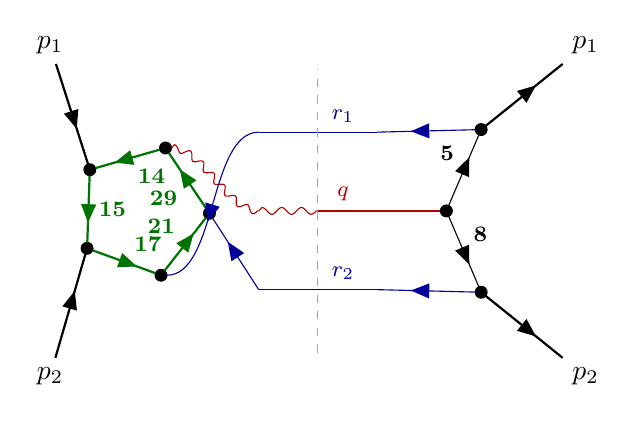
\begin{tikzpicture}
\begin{feynman}
\vertex (Lp1) at (-3.400,2.100) {$p_1$};
\vertex (Lp2) at (-3.400,-2.100) {$p_2$};
\vertex (Lcr1) at (-0.750,1.000);
\vertex (Lcr2) at (-0.750,-1.000);
\vertex (Lcq) at (-0.750,0.000);
\vertex (Mq) at (0,0.000);
\vertex[dot] (Lv0) at (-1.934,0.799) {};
\vertex[dot] (Lv1) at (-2.895,0.523) {};
\vertex[dot] (Lv2) at (-2.930,-0.475) {};
\vertex[dot] (Lv3) at (-1.991,-0.817) {};
\vertex[dot] (Lv4) at (-1.376,-0.030) {};
\vertex (Rp1) at (3.400,2.100) {$p_1$};
\vertex (Rp2) at (3.400,-2.100) {$p_2$};
\vertex (Rcr1) at (0.750,1.000);
\vertex (Rcr2) at (0.750,-1.000);
\vertex (Rcq) at (0.750,0.000);
\vertex[dot] (R5) at (2.075,1.033) {};
\vertex[dot] (Rroot) at (1.633,0.000) {};
\vertex[dot] (R8) at (2.075,-1.033) {};
\diagram* {
(Lv0) -- [plain, thick, green!45!black, with arrow=0.55, edge label={\footnotesize\bfseries 14}] (Lv1),
(Lv1) -- [plain, thick, green!45!black, with arrow=0.55, edge label={\footnotesize\bfseries 15}] (Lv2),
(Lv2) -- [plain, thick, green!45!black, with arrow=0.55, edge label={\footnotesize\bfseries 17}] (Lv3),
(Lv3) -- [plain, thick, green!45!black, with arrow=0.55, edge label={\footnotesize\bfseries 21}] (Lv4),
(Lv4) -- [plain, thick, green!45!black, with arrow=0.55, edge label={\footnotesize\bfseries 29}] (Lv0),
(Lcq) -- [boson, red!70!black, out=180, in=0, looseness=0.75] (Lv0),
(Lp1) -- [plain, thick, with arrow=0.55] (Lv1),
(Lp2) -- [plain, thick, with arrow=0.55] (Lv2),
(Lcr1) -- [plain, blue!60!black, out=180, in=0, looseness=0.75, with arrow=0.55] (Lv3),
(Lcr2) -- [plain, blue!60!black, with arrow=0.55] (Lv4),
(Rroot) -- [plain, with arrow=0.55, edge label={\footnotesize\bfseries 5}] (R5),
(Rroot) -- [plain, with arrow=0.55, edge label={\footnotesize\bfseries 8}] (R8),
(R5) -- [plain, thick, with arrow=0.55] (Rp1),
(R8) -- [plain, thick, with arrow=0.55] (Rp2),
(R5) -- [plain, blue!60!black, with arrow=0.55] (Rcr1),
(R8) -- [plain, blue!60!black, with arrow=0.55] (Rcr2),
(Rroot) -- [plain, red!70!black, double, double distance=1.2pt, thick] (Rcq),
(Rcr1) -- [plain, blue!60!black] (Lcr1),
(Rcr2) -- [plain, blue!60!black] (Lcr2),
(Rcq) -- [plain, red!70!black, double, double distance=1.2pt, thick] (Mq) -- [boson, red!70!black] (Lcq),
};
\end{feynman}
\draw[dashed, gray!70] (0,-1.80) -- (0,1.80);
\node[font=\footnotesize, blue!60!black, above] at (0.32,1.00) {$r_1$};
\node[font=\footnotesize, blue!60!black, above] at (0.32,-1.00) {$r_2$};
\node[font=\footnotesize, red!70!black, above] at (0.32,0.00) {$q$};
\end{tikzpicture}}\\[2mm]\textbf{topo46} (RR family 7, pentagon q-p1-p2-r1-r2)\\[2pt]{\footnotesize\begin{tabular}{@{}r@{\ \ }l@{\ \ }l@{}}\textbf{14} & $(k_1)^2$ & loop\\
\textbf{15} & $(k_1+p_1)^2$ & loop\\
\textbf{17} & $(k_1+p_1+p_2)^2$ & loop\\
\textbf{21} & $(k_1+p_1+p_2+r_1)^2$ & loop\\
\textbf{29} & $(k_1+p_1+p_2+r_1+r_2)^2$ & loop\\
\textbf{5} & $(p_1+r_1)^2$ & conjugate\\
\textbf{8} & $(p_2+r_2)^2$ & conjugate\\
\textbf{10} & $(p_2+r_1+r_2)^2$ & \textcolor{red}{irreducible numerator}\\\end{tabular}}\end{minipage}

\bigskip

\begin{minipage}[t]{0.48\textwidth}\centering\resizebox{0.9\linewidth}{!}{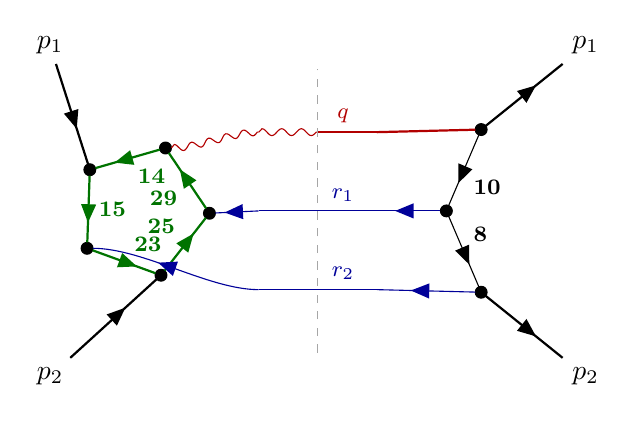
\begin{tikzpicture}
\begin{feynman}
\vertex (Lp1) at (-3.400,2.100) {$p_1$};
\vertex (Lp2) at (-3.400,-2.100) {$p_2$};
\vertex (Lcr1) at (-0.750,0.000);
\vertex (Lcr2) at (-0.750,-1.000);
\vertex (Lcq) at (-0.750,1.000);
\vertex (Mq) at (0,1.000);
\vertex[dot] (Lv0) at (-1.934,0.799) {};
\vertex[dot] (Lv1) at (-2.895,0.523) {};
\vertex[dot] (Lv2) at (-2.930,-0.475) {};
\vertex[dot] (Lv3) at (-1.991,-0.817) {};
\vertex[dot] (Lv4) at (-1.376,-0.030) {};
\vertex (Rp1) at (3.400,2.100) {$p_1$};
\vertex (Rp2) at (3.400,-2.100) {$p_2$};
\vertex (Rcr1) at (0.750,0.000);
\vertex (Rcr2) at (0.750,-1.000);
\vertex (Rcq) at (0.750,1.000);
\vertex[dot] (R8) at (2.075,-1.033) {};
\vertex[dot] (R10) at (1.633,0.000) {};
\vertex[dot] (Rroot) at (2.075,1.033) {};
\diagram* {
(Lv0) -- [plain, thick, green!45!black, with arrow=0.55, edge label={\footnotesize\bfseries 14}] (Lv1),
(Lv1) -- [plain, thick, green!45!black, with arrow=0.55, edge label={\footnotesize\bfseries 15}] (Lv2),
(Lv2) -- [plain, thick, green!45!black, with arrow=0.55, edge label={\footnotesize\bfseries 23}] (Lv3),
(Lv3) -- [plain, thick, green!45!black, with arrow=0.55, edge label={\footnotesize\bfseries 25}] (Lv4),
(Lv4) -- [plain, thick, green!45!black, with arrow=0.55, edge label={\footnotesize\bfseries 29}] (Lv0),
(Lcq) -- [boson, red!70!black, out=180, in=0, looseness=0.75] (Lv0),
(Lp1) -- [plain, thick, with arrow=0.55] (Lv1),
(Lcr2) -- [plain, blue!60!black, out=180, in=0, looseness=0.75, with arrow=0.55] (Lv2),
(Lp2) -- [plain, thick, with arrow=0.55] (Lv3),
(Lcr1) -- [plain, blue!60!black, with arrow=0.55] (Lv4),
(R10) -- [plain, with arrow=0.55, edge label={\footnotesize\bfseries 8}] (R8),
(Rroot) -- [plain, with arrow=0.55, edge label={\footnotesize\bfseries 10}] (R10),
(Rroot) -- [plain, thick, with arrow=0.55] (Rp1),
(R8) -- [plain, thick, with arrow=0.55] (Rp2),
(R10) -- [plain, blue!60!black, with arrow=0.55] (Rcr1),
(R8) -- [plain, blue!60!black, with arrow=0.55] (Rcr2),
(Rroot) -- [plain, red!70!black, double, double distance=1.2pt, thick] (Rcq),
(Rcr1) -- [plain, blue!60!black] (Lcr1),
(Rcr2) -- [plain, blue!60!black] (Lcr2),
(Rcq) -- [plain, red!70!black, double, double distance=1.2pt, thick] (Mq) -- [boson, red!70!black] (Lcq),
};
\end{feynman}
\draw[dashed, gray!70] (0,-1.80) -- (0,1.80);
\node[font=\footnotesize, blue!60!black, above] at (0.32,0.00) {$r_1$};
\node[font=\footnotesize, blue!60!black, above] at (0.32,-1.00) {$r_2$};
\node[font=\footnotesize, red!70!black, above] at (0.32,1.00) {$q$};
\end{tikzpicture}}\\[2mm]\textbf{topo47} (RR family 29, pentagon q-p1-r2-p2-r1)\\[2pt]{\footnotesize\begin{tabular}{@{}r@{\ \ }l@{\ \ }l@{}}\textbf{14} & $(k_1)^2$ & loop\\
\textbf{15} & $(k_1+p_1)^2$ & loop\\
\textbf{23} & $(k_1+p_1+r_2)^2$ & loop\\
\textbf{25} & $(k_1+p_1+p_2+r_2)^2$ & loop\\
\textbf{29} & $(k_1+p_1+p_2+r_1+r_2)^2$ & loop\\
\textbf{8} & $(p_2+r_2)^2$ & conjugate\\
\textbf{10} & $(p_2+r_1+r_2)^2$ & conjugate\\
\textbf{13} & $(p_1+p_2+r_2)^2$ & \textcolor{red}{irreducible numerator}\\\end{tabular}}\end{minipage}\hfill%
\begin{minipage}[t]{0.48\textwidth}\centering\resizebox{0.9\linewidth}{!}{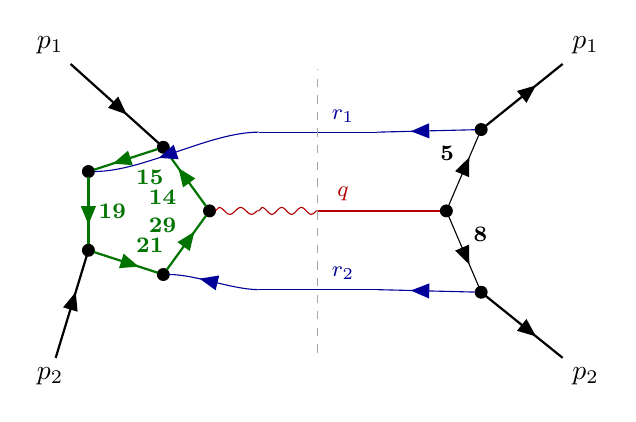
\begin{tikzpicture}
\begin{feynman}
\vertex (Lp1) at (-3.400,2.100) {$p_1$};
\vertex (Lp2) at (-3.400,-2.100) {$p_2$};
\vertex (Lcr1) at (-0.750,1.000);
\vertex (Lcr2) at (-0.750,-1.000);
\vertex (Lcq) at (-0.750,0.000);
\vertex (Mq) at (0,0.000);
\vertex[dot] (Lv0) at (-1.375,0.000) {};
\vertex[dot] (Lv1) at (-1.962,0.808) {};
\vertex[dot] (Lv2) at (-2.913,0.500) {};
\vertex[dot] (Lv3) at (-2.913,-0.500) {};
\vertex[dot] (Lv4) at (-1.962,-0.808) {};
\vertex (Rp1) at (3.400,2.100) {$p_1$};
\vertex (Rp2) at (3.400,-2.100) {$p_2$};
\vertex (Rcr1) at (0.750,1.000);
\vertex (Rcr2) at (0.750,-1.000);
\vertex (Rcq) at (0.750,0.000);
\vertex[dot] (R5) at (2.075,1.033) {};
\vertex[dot] (Rroot) at (1.633,0.000) {};
\vertex[dot] (R8) at (2.075,-1.033) {};
\diagram* {
(Lv0) -- [plain, thick, green!45!black, with arrow=0.55, edge label={\footnotesize\bfseries 14}] (Lv1),
(Lv1) -- [plain, thick, green!45!black, with arrow=0.55, edge label={\footnotesize\bfseries 15}] (Lv2),
(Lv2) -- [plain, thick, green!45!black, with arrow=0.55, edge label={\footnotesize\bfseries 19}] (Lv3),
(Lv3) -- [plain, thick, green!45!black, with arrow=0.55, edge label={\footnotesize\bfseries 21}] (Lv4),
(Lv4) -- [plain, thick, green!45!black, with arrow=0.55, edge label={\footnotesize\bfseries 29}] (Lv0),
(Lcq) -- [boson, red!70!black] (Lv0),
(Lp1) -- [plain, thick, with arrow=0.55] (Lv1),
(Lcr1) -- [plain, blue!60!black, out=180, in=0, looseness=0.75, with arrow=0.55] (Lv2),
(Lp2) -- [plain, thick, with arrow=0.55] (Lv3),
(Lcr2) -- [plain, blue!60!black, out=180, in=0, looseness=0.75, with arrow=0.55] (Lv4),
(Rroot) -- [plain, with arrow=0.55, edge label={\footnotesize\bfseries 5}] (R5),
(Rroot) -- [plain, with arrow=0.55, edge label={\footnotesize\bfseries 8}] (R8),
(R5) -- [plain, thick, with arrow=0.55] (Rp1),
(R8) -- [plain, thick, with arrow=0.55] (Rp2),
(R5) -- [plain, blue!60!black, with arrow=0.55] (Rcr1),
(R8) -- [plain, blue!60!black, with arrow=0.55] (Rcr2),
(Rroot) -- [plain, red!70!black, double, double distance=1.2pt, thick] (Rcq),
(Rcr1) -- [plain, blue!60!black] (Lcr1),
(Rcr2) -- [plain, blue!60!black] (Lcr2),
(Rcq) -- [plain, red!70!black, double, double distance=1.2pt, thick] (Mq) -- [boson, red!70!black] (Lcq),
};
\end{feynman}
\draw[dashed, gray!70] (0,-1.80) -- (0,1.80);
\node[font=\footnotesize, blue!60!black, above] at (0.32,1.00) {$r_1$};
\node[font=\footnotesize, blue!60!black, above] at (0.32,-1.00) {$r_2$};
\node[font=\footnotesize, red!70!black, above] at (0.32,0.00) {$q$};
\end{tikzpicture}}\\[2mm]\textbf{topo48} (RR family 17, pentagon q-p1-r1-p2-r2)\\[2pt]{\footnotesize\begin{tabular}{@{}r@{\ \ }l@{\ \ }l@{}}\textbf{14} & $(k_1)^2$ & loop\\
\textbf{15} & $(k_1+p_1)^2$ & loop\\
\textbf{19} & $(k_1+p_1+r_1)^2$ & loop\\
\textbf{21} & $(k_1+p_1+p_2+r_1)^2$ & loop\\
\textbf{29} & $(k_1+p_1+p_2+r_1+r_2)^2$ & loop\\
\textbf{5} & $(p_1+r_1)^2$ & conjugate\\
\textbf{8} & $(p_2+r_2)^2$ & conjugate\\
\textbf{12} & $(p_1+p_2+r_1)^2$ & \textcolor{red}{irreducible numerator}\\\end{tabular}}\end{minipage}

\bigskip

\begin{minipage}[t]{0.48\textwidth}\centering\resizebox{0.9\linewidth}{!}{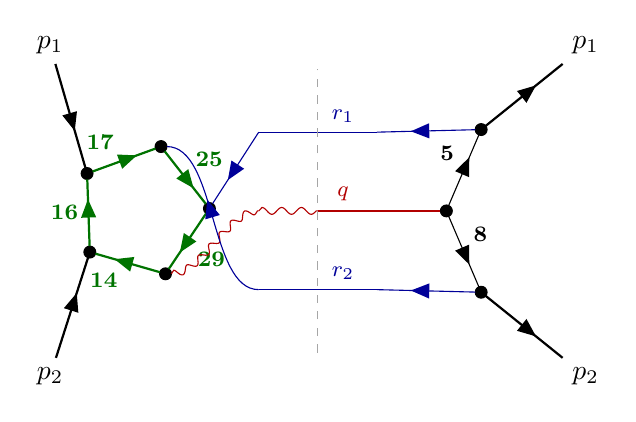
\begin{tikzpicture}
\begin{feynman}
\vertex (Lp1) at (-3.400,2.100) {$p_1$};
\vertex (Lp2) at (-3.400,-2.100) {$p_2$};
\vertex (Lcr1) at (-0.750,1.000);
\vertex (Lcr2) at (-0.750,-1.000);
\vertex (Lcq) at (-0.750,0.000);
\vertex (Mq) at (0,0.000);
\vertex[dot] (Lv0) at (-1.934,-0.799) {};
\vertex[dot] (Lv1) at (-2.895,-0.523) {};
\vertex[dot] (Lv2) at (-2.930,0.475) {};
\vertex[dot] (Lv3) at (-1.991,0.817) {};
\vertex[dot] (Lv4) at (-1.376,0.030) {};
\vertex (Rp1) at (3.400,2.100) {$p_1$};
\vertex (Rp2) at (3.400,-2.100) {$p_2$};
\vertex (Rcr1) at (0.750,1.000);
\vertex (Rcr2) at (0.750,-1.000);
\vertex (Rcq) at (0.750,0.000);
\vertex[dot] (R5) at (2.075,1.033) {};
\vertex[dot] (Rroot) at (1.633,0.000) {};
\vertex[dot] (R8) at (2.075,-1.033) {};
\diagram* {
(Lv0) -- [plain, thick, green!45!black, with arrow=0.55, edge label={\footnotesize\bfseries 14}] (Lv1),
(Lv1) -- [plain, thick, green!45!black, with arrow=0.55, edge label={\footnotesize\bfseries 16}] (Lv2),
(Lv2) -- [plain, thick, green!45!black, with arrow=0.55, edge label={\footnotesize\bfseries 17}] (Lv3),
(Lv3) -- [plain, thick, green!45!black, with arrow=0.55, edge label={\footnotesize\bfseries 25}] (Lv4),
(Lv4) -- [plain, thick, green!45!black, with arrow=0.55, edge label={\footnotesize\bfseries 29}] (Lv0),
(Lcq) -- [boson, red!70!black, out=180, in=0, looseness=0.75] (Lv0),
(Lp2) -- [plain, thick, with arrow=0.55] (Lv1),
(Lp1) -- [plain, thick, with arrow=0.55] (Lv2),
(Lcr2) -- [plain, blue!60!black, out=180, in=0, looseness=0.75, with arrow=0.55] (Lv3),
(Lcr1) -- [plain, blue!60!black, with arrow=0.55] (Lv4),
(Rroot) -- [plain, with arrow=0.55, edge label={\footnotesize\bfseries 5}] (R5),
(Rroot) -- [plain, with arrow=0.55, edge label={\footnotesize\bfseries 8}] (R8),
(R5) -- [plain, thick, with arrow=0.55] (Rp1),
(R8) -- [plain, thick, with arrow=0.55] (Rp2),
(R5) -- [plain, blue!60!black, with arrow=0.55] (Rcr1),
(R8) -- [plain, blue!60!black, with arrow=0.55] (Rcr2),
(Rroot) -- [plain, red!70!black, double, double distance=1.2pt, thick] (Rcq),
(Rcr1) -- [plain, blue!60!black] (Lcr1),
(Rcr2) -- [plain, blue!60!black] (Lcr2),
(Rcq) -- [plain, red!70!black, double, double distance=1.2pt, thick] (Mq) -- [boson, red!70!black] (Lcq),
};
\end{feynman}
\draw[dashed, gray!70] (0,-1.80) -- (0,1.80);
\node[font=\footnotesize, blue!60!black, above] at (0.32,1.00) {$r_1$};
\node[font=\footnotesize, blue!60!black, above] at (0.32,-1.00) {$r_2$};
\node[font=\footnotesize, red!70!black, above] at (0.32,0.00) {$q$};
\end{tikzpicture}}\\[2mm]\textbf{topo49} (RR family 6, pentagon q-p2-p1-r2-r1)\\[2pt]{\footnotesize\begin{tabular}{@{}r@{\ \ }l@{\ \ }l@{}}\textbf{14} & $(k_1)^2$ & loop\\
\textbf{16} & $(k_1+p_2)^2$ & loop\\
\textbf{17} & $(k_1+p_1+p_2)^2$ & loop\\
\textbf{25} & $(k_1+p_1+p_2+r_2)^2$ & loop\\
\textbf{29} & $(k_1+p_1+p_2+r_1+r_2)^2$ & loop\\
\textbf{5} & $(p_1+r_1)^2$ & conjugate\\
\textbf{8} & $(p_2+r_2)^2$ & conjugate\\
\textbf{9} & $(p_1+r_1+r_2)^2$ & \textcolor{red}{irreducible numerator}\\\end{tabular}}\end{minipage}\hfill%
\begin{minipage}[t]{0.48\textwidth}\centering\resizebox{0.9\linewidth}{!}{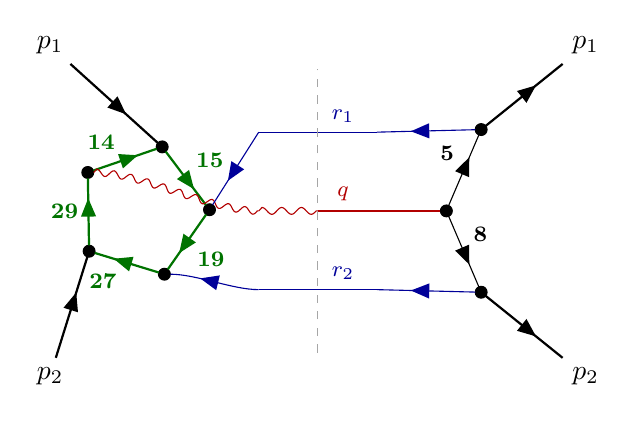
\begin{tikzpicture}
\begin{feynman}
\vertex (Lp1) at (-3.400,2.100) {$p_1$};
\vertex (Lp2) at (-3.400,-2.100) {$p_2$};
\vertex (Lcr1) at (-0.750,1.000);
\vertex (Lcr2) at (-0.750,-1.000);
\vertex (Lcq) at (-0.750,0.000);
\vertex (Mq) at (0,0.000);
\vertex[dot] (Lv0) at (-2.921,0.488) {};
\vertex[dot] (Lv1) at (-1.976,0.813) {};
\vertex[dot] (Lv2) at (-1.375,0.015) {};
\vertex[dot] (Lv3) at (-1.948,-0.804) {};
\vertex[dot] (Lv4) at (-2.904,-0.512) {};
\vertex (Rp1) at (3.400,2.100) {$p_1$};
\vertex (Rp2) at (3.400,-2.100) {$p_2$};
\vertex (Rcr1) at (0.750,1.000);
\vertex (Rcr2) at (0.750,-1.000);
\vertex (Rcq) at (0.750,0.000);
\vertex[dot] (R5) at (2.075,1.033) {};
\vertex[dot] (Rroot) at (1.633,0.000) {};
\vertex[dot] (R8) at (2.075,-1.033) {};
\diagram* {
(Lv0) -- [plain, thick, green!45!black, with arrow=0.55, edge label={\footnotesize\bfseries 14}] (Lv1),
(Lv1) -- [plain, thick, green!45!black, with arrow=0.55, edge label={\footnotesize\bfseries 15}] (Lv2),
(Lv2) -- [plain, thick, green!45!black, with arrow=0.55, edge label={\footnotesize\bfseries 19}] (Lv3),
(Lv3) -- [plain, thick, green!45!black, with arrow=0.55, edge label={\footnotesize\bfseries 27}] (Lv4),
(Lv4) -- [plain, thick, green!45!black, with arrow=0.55, edge label={\footnotesize\bfseries 29}] (Lv0),
(Lcq) -- [boson, red!70!black, out=180, in=0, looseness=0.75] (Lv0),
(Lp1) -- [plain, thick, with arrow=0.55] (Lv1),
(Lcr1) -- [plain, blue!60!black, with arrow=0.55] (Lv2),
(Lcr2) -- [plain, blue!60!black, out=180, in=0, looseness=0.75, with arrow=0.55] (Lv3),
(Lp2) -- [plain, thick, with arrow=0.55] (Lv4),
(Rroot) -- [plain, with arrow=0.55, edge label={\footnotesize\bfseries 5}] (R5),
(Rroot) -- [plain, with arrow=0.55, edge label={\footnotesize\bfseries 8}] (R8),
(R5) -- [plain, thick, with arrow=0.55] (Rp1),
(R8) -- [plain, thick, with arrow=0.55] (Rp2),
(R5) -- [plain, blue!60!black, with arrow=0.55] (Rcr1),
(R8) -- [plain, blue!60!black, with arrow=0.55] (Rcr2),
(Rroot) -- [plain, red!70!black, double, double distance=1.2pt, thick] (Rcq),
(Rcr1) -- [plain, blue!60!black] (Lcr1),
(Rcr2) -- [plain, blue!60!black] (Lcr2),
(Rcq) -- [plain, red!70!black, double, double distance=1.2pt, thick] (Mq) -- [boson, red!70!black] (Lcq),
};
\end{feynman}
\draw[dashed, gray!70] (0,-1.80) -- (0,1.80);
\node[font=\footnotesize, blue!60!black, above] at (0.32,1.00) {$r_1$};
\node[font=\footnotesize, blue!60!black, above] at (0.32,-1.00) {$r_2$};
\node[font=\footnotesize, red!70!black, above] at (0.32,0.00) {$q$};
\end{tikzpicture}}\\[2mm]\textbf{topo50} (RR family 7, pentagon q-p1-r1-r2-p2)\\[2pt]{\footnotesize\begin{tabular}{@{}r@{\ \ }l@{\ \ }l@{}}\textbf{14} & $(k_1)^2$ & loop\\
\textbf{15} & $(k_1+p_1)^2$ & loop\\
\textbf{19} & $(k_1+p_1+r_1)^2$ & loop\\
\textbf{27} & $(k_1+p_1+r_1+r_2)^2$ & loop\\
\textbf{29} & $(k_1+p_1+p_2+r_1+r_2)^2$ & loop\\
\textbf{5} & $(p_1+r_1)^2$ & conjugate\\
\textbf{8} & $(p_2+r_2)^2$ & conjugate\\
\textbf{10} & $(p_2+r_1+r_2)^2$ & \textcolor{red}{irreducible numerator}\\\end{tabular}}\end{minipage}

\bigskip

\begin{minipage}[t]{0.48\textwidth}\centering\resizebox{0.9\linewidth}{!}{\begin{tikzpicture}
\begin{feynman}
\vertex (Lp1) at (-3.400,2.100) {$p_1$};
\vertex (Lp2) at (-3.400,-2.100) {$p_2$};
\vertex (Lcr1) at (-0.750,0.000);
\vertex (Lcr2) at (-0.750,1.000);
\vertex (Lcq) at (-0.750,-1.000);
\vertex (Mq) at (0,-1.000);
\vertex[dot] (Lv0) at (-2.921,-0.488) {};
\vertex[dot] (Lv1) at (-2.904,0.512) {};
\vertex[dot] (Lv2) at (-1.948,0.804) {};
\vertex[dot] (Lv3) at (-1.375,-0.015) {};
\vertex[dot] (Lv4) at (-1.976,-0.813) {};
\vertex (Rp1) at (3.400,2.100) {$p_1$};
\vertex (Rp2) at (3.400,-2.100) {$p_2$};
\vertex (Rcr1) at (0.750,0.000);
\vertex (Rcr2) at (0.750,1.000);
\vertex (Rcq) at (0.750,-1.000);
\vertex[dot] (R7) at (2.075,1.033) {};
\vertex[dot] (R9) at (1.633,0.000) {};
\vertex[dot] (Rroot) at (2.075,-1.033) {};
\diagram* {
(Lv0) -- [plain, thick, green!45!black, with arrow=0.55, edge label={\footnotesize\bfseries 14}] (Lv1),
(Lv1) -- [plain, thick, green!45!black, with arrow=0.55, edge label={\footnotesize\bfseries 15}] (Lv2),
(Lv2) -- [plain, thick, green!45!black, with arrow=0.55, edge label={\footnotesize\bfseries 19}] (Lv3),
(Lv3) -- [plain, thick, green!45!black, with arrow=0.55, edge label={\footnotesize\bfseries 27}] (Lv4),
(Lv4) -- [plain, thick, green!45!black, with arrow=0.55, edge label={\footnotesize\bfseries 29}] (Lv0),
(Lcq) -- [boson, red!70!black, out=180, in=0, looseness=0.75] (Lv0),
(Lp1) -- [plain, thick, with arrow=0.55] (Lv1),
(Lcr1) -- [plain, blue!60!black, out=180, in=0, looseness=0.75, with arrow=0.55] (Lv2),
(Lcr2) -- [plain, blue!60!black, with arrow=0.55] (Lv3),
(Lp2) -- [plain, thick, with arrow=0.55] (Lv4),
(R9) -- [plain, with arrow=0.55, edge label={\footnotesize\bfseries 7}] (R7),
(Rroot) -- [plain, with arrow=0.55, edge label={\footnotesize\bfseries 9}] (R9),
(R7) -- [plain, thick, with arrow=0.55] (Rp1),
(Rroot) -- [plain, thick, with arrow=0.55] (Rp2),
(R9) -- [plain, blue!60!black, with arrow=0.55] (Rcr1),
(R7) -- [plain, blue!60!black, with arrow=0.55] (Rcr2),
(Rroot) -- [plain, red!70!black, double, double distance=1.2pt, thick] (Rcq),
(Rcr1) -- [plain, blue!60!black] (Lcr1),
(Rcr2) -- [plain, blue!60!black] (Lcr2),
(Rcq) -- [plain, red!70!black, double, double distance=1.2pt, thick] (Mq) -- [boson, red!70!black] (Lcq),
};
\end{feynman}
\draw[dashed, gray!70] (0,-1.80) -- (0,1.80);
\node[font=\footnotesize, blue!60!black, above] at (0.32,0.00) {$r_1$};
\node[font=\footnotesize, blue!60!black, above] at (0.32,1.00) {$r_2$};
\node[font=\footnotesize, red!70!black, above] at (0.32,-1.00) {$q$};
\end{tikzpicture}}\\[2mm]\textbf{topo51} (RR family 33, pentagon q-p1-r1-r2-p2)\\[2pt]{\footnotesize\begin{tabular}{@{}r@{\ \ }l@{\ \ }l@{}}\textbf{14} & $(k_1)^2$ & loop\\
\textbf{15} & $(k_1+p_1)^2$ & loop\\
\textbf{19} & $(k_1+p_1+r_1)^2$ & loop\\
\textbf{27} & $(k_1+p_1+r_1+r_2)^2$ & loop\\
\textbf{29} & $(k_1+p_1+p_2+r_1+r_2)^2$ & loop\\
\textbf{7} & $(p_1+r_2)^2$ & conjugate\\
\textbf{9} & $(p_1+r_1+r_2)^2$ & conjugate\\
\textbf{13} & $(p_1+p_2+r_2)^2$ & \textcolor{red}{irreducible numerator}\\\end{tabular}}\end{minipage}\hfill%
\begin{minipage}[t]{0.48\textwidth}\centering\resizebox{0.9\linewidth}{!}{\begin{tikzpicture}
\begin{feynman}
\vertex (Lp1) at (-3.400,2.100) {$p_1$};
\vertex (Lp2) at (-3.400,-2.100) {$p_2$};
\vertex (Lcr1) at (-0.750,1.000);
\vertex (Lcr2) at (-0.750,-1.000);
\vertex (Lcq) at (-0.750,0.000);
\vertex (Mq) at (0,0.000);
\vertex[dot] (Lv0) at (-1.375,0.000) {};
\vertex[dot] (Lv1) at (-1.962,-0.808) {};
\vertex[dot] (Lv2) at (-2.913,-0.500) {};
\vertex[dot] (Lv3) at (-2.913,0.500) {};
\vertex[dot] (Lv4) at (-1.962,0.808) {};
\vertex (Rp1) at (3.400,2.100) {$p_1$};
\vertex (Rp2) at (3.400,-2.100) {$p_2$};
\vertex (Rcr1) at (0.750,1.000);
\vertex (Rcr2) at (0.750,-1.000);
\vertex (Rcq) at (0.750,0.000);
\vertex[dot] (R5) at (2.075,1.033) {};
\vertex[dot] (Rroot) at (1.633,0.000) {};
\vertex[dot] (R8) at (2.075,-1.033) {};
\diagram* {
(Lv0) -- [plain, thick, green!45!black, with arrow=0.55, edge label={\footnotesize\bfseries 14}] (Lv1),
(Lv1) -- [plain, thick, green!45!black, with arrow=0.55, edge label={\footnotesize\bfseries 16}] (Lv2),
(Lv2) -- [plain, thick, green!45!black, with arrow=0.55, edge label={\footnotesize\bfseries 24}] (Lv3),
(Lv3) -- [plain, thick, green!45!black, with arrow=0.55, edge label={\footnotesize\bfseries 25}] (Lv4),
(Lv4) -- [plain, thick, green!45!black, with arrow=0.55, edge label={\footnotesize\bfseries 29}] (Lv0),
(Lcq) -- [boson, red!70!black] (Lv0),
(Lp2) -- [plain, thick, with arrow=0.55] (Lv1),
(Lcr2) -- [plain, blue!60!black, out=180, in=0, looseness=0.75, with arrow=0.55] (Lv2),
(Lp1) -- [plain, thick, with arrow=0.55] (Lv3),
(Lcr1) -- [plain, blue!60!black, out=180, in=0, looseness=0.75, with arrow=0.55] (Lv4),
(Rroot) -- [plain, with arrow=0.55, edge label={\footnotesize\bfseries 5}] (R5),
(Rroot) -- [plain, with arrow=0.55, edge label={\footnotesize\bfseries 8}] (R8),
(R5) -- [plain, thick, with arrow=0.55] (Rp1),
(R8) -- [plain, thick, with arrow=0.55] (Rp2),
(R5) -- [plain, blue!60!black, with arrow=0.55] (Rcr1),
(R8) -- [plain, blue!60!black, with arrow=0.55] (Rcr2),
(Rroot) -- [plain, red!70!black, double, double distance=1.2pt, thick] (Rcq),
(Rcr1) -- [plain, blue!60!black] (Lcr1),
(Rcr2) -- [plain, blue!60!black] (Lcr2),
(Rcq) -- [plain, red!70!black, double, double distance=1.2pt, thick] (Mq) -- [boson, red!70!black] (Lcq),
};
\end{feynman}
\draw[dashed, gray!70] (0,-1.80) -- (0,1.80);
\node[font=\footnotesize, blue!60!black, above] at (0.32,1.00) {$r_1$};
\node[font=\footnotesize, blue!60!black, above] at (0.32,-1.00) {$r_2$};
\node[font=\footnotesize, red!70!black, above] at (0.32,0.00) {$q$};
\end{tikzpicture}}\\[2mm]\textbf{topo52} (RR family 8, pentagon q-p2-r2-p1-r1)\\[2pt]{\footnotesize\begin{tabular}{@{}r@{\ \ }l@{\ \ }l@{}}\textbf{14} & $(k_1)^2$ & loop\\
\textbf{16} & $(k_1+p_2)^2$ & loop\\
\textbf{24} & $(k_1+p_2+r_2)^2$ & loop\\
\textbf{25} & $(k_1+p_1+p_2+r_2)^2$ & loop\\
\textbf{29} & $(k_1+p_1+p_2+r_1+r_2)^2$ & loop\\
\textbf{5} & $(p_1+r_1)^2$ & conjugate\\
\textbf{8} & $(p_2+r_2)^2$ & conjugate\\
\textbf{11} & $(r_1+r_2)^2$ & \textcolor{red}{irreducible numerator}\\\end{tabular}}\end{minipage}

\bigskip

\begin{minipage}[t]{0.48\textwidth}\centering\resizebox{0.9\linewidth}{!}{\begin{tikzpicture}
\begin{feynman}
\vertex (Lp1) at (-3.400,2.100) {$p_1$};
\vertex (Lp2) at (-3.400,-2.100) {$p_2$};
\vertex (Lcr1) at (-0.750,1.000);
\vertex (Lcr2) at (-0.750,-1.000);
\vertex (Lcq) at (-0.750,0.000);
\vertex (Mq) at (0,0.000);
\vertex[dot] (Lv0) at (-1.934,-0.799) {};
\vertex[dot] (Lv1) at (-2.895,-0.523) {};
\vertex[dot] (Lv2) at (-2.930,0.475) {};
\vertex[dot] (Lv3) at (-1.991,0.817) {};
\vertex[dot] (Lv4) at (-1.376,0.030) {};
\vertex (Rp1) at (3.400,2.100) {$p_1$};
\vertex (Rp2) at (3.400,-2.100) {$p_2$};
\vertex (Rcr1) at (0.750,1.000);
\vertex (Rcr2) at (0.750,-1.000);
\vertex (Rcq) at (0.750,0.000);
\vertex[dot] (R5) at (2.075,1.033) {};
\vertex[dot] (Rroot) at (1.633,0.000) {};
\vertex[dot] (R8) at (2.075,-1.033) {};
\diagram* {
(Lv0) -- [plain, thick, green!45!black, with arrow=0.55, edge label={\footnotesize\bfseries 14}] (Lv1),
(Lv1) -- [plain, thick, green!45!black, with arrow=0.55, edge label={\footnotesize\bfseries 16}] (Lv2),
(Lv2) -- [plain, thick, green!45!black, with arrow=0.55, edge label={\footnotesize\bfseries 20}] (Lv3),
(Lv3) -- [plain, thick, green!45!black, with arrow=0.55, edge label={\footnotesize\bfseries 21}] (Lv4),
(Lv4) -- [plain, thick, green!45!black, with arrow=0.55, edge label={\footnotesize\bfseries 29}] (Lv0),
(Lcq) -- [boson, red!70!black, out=180, in=0, looseness=0.75] (Lv0),
(Lp2) -- [plain, thick, with arrow=0.55] (Lv1),
(Lcr1) -- [plain, blue!60!black, out=180, in=0, looseness=0.75, with arrow=0.55] (Lv2),
(Lp1) -- [plain, thick, with arrow=0.55] (Lv3),
(Lcr2) -- [plain, blue!60!black, with arrow=0.55] (Lv4),
(Rroot) -- [plain, with arrow=0.55, edge label={\footnotesize\bfseries 5}] (R5),
(Rroot) -- [plain, with arrow=0.55, edge label={\footnotesize\bfseries 8}] (R8),
(R5) -- [plain, thick, with arrow=0.55] (Rp1),
(R8) -- [plain, thick, with arrow=0.55] (Rp2),
(R5) -- [plain, blue!60!black, with arrow=0.55] (Rcr1),
(R8) -- [plain, blue!60!black, with arrow=0.55] (Rcr2),
(Rroot) -- [plain, red!70!black, double, double distance=1.2pt, thick] (Rcq),
(Rcr1) -- [plain, blue!60!black] (Lcr1),
(Rcr2) -- [plain, blue!60!black] (Lcr2),
(Rcq) -- [plain, red!70!black, double, double distance=1.2pt, thick] (Mq) -- [boson, red!70!black] (Lcq),
};
\end{feynman}
\draw[dashed, gray!70] (0,-1.80) -- (0,1.80);
\node[font=\footnotesize, blue!60!black, above] at (0.32,1.00) {$r_1$};
\node[font=\footnotesize, blue!60!black, above] at (0.32,-1.00) {$r_2$};
\node[font=\footnotesize, red!70!black, above] at (0.32,0.00) {$q$};
\end{tikzpicture}}\\[2mm]\textbf{topo53} (RR family 2, pentagon q-p2-r1-p1-r2)\\[2pt]{\footnotesize\begin{tabular}{@{}r@{\ \ }l@{\ \ }l@{}}\textbf{14} & $(k_1)^2$ & loop\\
\textbf{16} & $(k_1+p_2)^2$ & loop\\
\textbf{20} & $(k_1+p_2+r_1)^2$ & loop\\
\textbf{21} & $(k_1+p_1+p_2+r_1)^2$ & loop\\
\textbf{29} & $(k_1+p_1+p_2+r_1+r_2)^2$ & loop\\
\textbf{5} & $(p_1+r_1)^2$ & conjugate\\
\textbf{8} & $(p_2+r_2)^2$ & conjugate\\
\textbf{6} & $(p_2+r_1)^2$ & \textcolor{red}{irreducible numerator}\\\end{tabular}}\end{minipage}\hfill%
\begin{minipage}[t]{0.48\textwidth}\centering\resizebox{0.9\linewidth}{!}{\begin{tikzpicture}
\begin{feynman}
\vertex (Lp1) at (-3.400,2.100) {$p_1$};
\vertex (Lp2) at (-3.400,-2.100) {$p_2$};
\vertex (Lcr1) at (-0.750,1.000);
\vertex (Lcr2) at (-0.750,0.000);
\vertex (Lcq) at (-0.750,-1.000);
\vertex (Mq) at (0,-1.000);
\vertex[dot] (Lv0) at (-1.934,-0.799) {};
\vertex[dot] (Lv1) at (-2.895,-0.523) {};
\vertex[dot] (Lv2) at (-2.930,0.475) {};
\vertex[dot] (Lv3) at (-1.991,0.817) {};
\vertex[dot] (Lv4) at (-1.376,0.030) {};
\vertex (Rp1) at (3.400,2.100) {$p_1$};
\vertex (Rp2) at (3.400,-2.100) {$p_2$};
\vertex (Rcr1) at (0.750,1.000);
\vertex (Rcr2) at (0.750,0.000);
\vertex (Rcq) at (0.750,-1.000);
\vertex[dot] (R5) at (2.075,1.033) {};
\vertex[dot] (R9) at (1.633,0.000) {};
\vertex[dot] (Rroot) at (2.075,-1.033) {};
\diagram* {
(Lv0) -- [plain, thick, green!45!black, with arrow=0.55, edge label={\footnotesize\bfseries 14}] (Lv1),
(Lv1) -- [plain, thick, green!45!black, with arrow=0.55, edge label={\footnotesize\bfseries 16}] (Lv2),
(Lv2) -- [plain, thick, green!45!black, with arrow=0.55, edge label={\footnotesize\bfseries 20}] (Lv3),
(Lv3) -- [plain, thick, green!45!black, with arrow=0.55, edge label={\footnotesize\bfseries 21}] (Lv4),
(Lv4) -- [plain, thick, green!45!black, with arrow=0.55, edge label={\footnotesize\bfseries 29}] (Lv0),
(Lcq) -- [boson, red!70!black, out=180, in=0, looseness=0.75] (Lv0),
(Lp2) -- [plain, thick, with arrow=0.55] (Lv1),
(Lcr1) -- [plain, blue!60!black, out=180, in=0, looseness=0.75, with arrow=0.55] (Lv2),
(Lp1) -- [plain, thick, with arrow=0.55] (Lv3),
(Lcr2) -- [plain, blue!60!black, with arrow=0.55] (Lv4),
(R9) -- [plain, with arrow=0.55, edge label={\footnotesize\bfseries 5}] (R5),
(Rroot) -- [plain, with arrow=0.55, edge label={\footnotesize\bfseries 9}] (R9),
(R5) -- [plain, thick, with arrow=0.55] (Rp1),
(Rroot) -- [plain, thick, with arrow=0.55] (Rp2),
(R5) -- [plain, blue!60!black, with arrow=0.55] (Rcr1),
(R9) -- [plain, blue!60!black, with arrow=0.55] (Rcr2),
(Rroot) -- [plain, red!70!black, double, double distance=1.2pt, thick] (Rcq),
(Rcr1) -- [plain, blue!60!black] (Lcr1),
(Rcr2) -- [plain, blue!60!black] (Lcr2),
(Rcq) -- [plain, red!70!black, double, double distance=1.2pt, thick] (Mq) -- [boson, red!70!black] (Lcq),
};
\end{feynman}
\draw[dashed, gray!70] (0,-1.80) -- (0,1.80);
\node[font=\footnotesize, blue!60!black, above] at (0.32,1.00) {$r_1$};
\node[font=\footnotesize, blue!60!black, above] at (0.32,0.00) {$r_2$};
\node[font=\footnotesize, red!70!black, above] at (0.32,-1.00) {$q$};
\end{tikzpicture}}\\[2mm]\textbf{topo54} (RR family 3, pentagon q-p2-r1-p1-r2)\\[2pt]{\footnotesize\begin{tabular}{@{}r@{\ \ }l@{\ \ }l@{}}\textbf{14} & $(k_1)^2$ & loop\\
\textbf{16} & $(k_1+p_2)^2$ & loop\\
\textbf{20} & $(k_1+p_2+r_1)^2$ & loop\\
\textbf{21} & $(k_1+p_1+p_2+r_1)^2$ & loop\\
\textbf{29} & $(k_1+p_1+p_2+r_1+r_2)^2$ & loop\\
\textbf{5} & $(p_1+r_1)^2$ & conjugate\\
\textbf{9} & $(p_1+r_1+r_2)^2$ & conjugate\\
\textbf{6} & $(p_2+r_1)^2$ & \textcolor{red}{irreducible numerator}\\\end{tabular}}\end{minipage}

\bigskip

\begin{minipage}[t]{0.48\textwidth}\centering\resizebox{0.9\linewidth}{!}{\begin{tikzpicture}
\begin{feynman}
\vertex (Lp1) at (-3.400,2.100) {$p_1$};
\vertex (Lp2) at (-3.400,-2.100) {$p_2$};
\vertex (Lcr1) at (-0.750,-1.000);
\vertex (Lcr2) at (-0.750,0.000);
\vertex (Lcq) at (-0.750,1.000);
\vertex (Mq) at (0,1.000);
\vertex[dot] (Lv0) at (-1.934,0.799) {};
\vertex[dot] (Lv1) at (-2.895,0.523) {};
\vertex[dot] (Lv2) at (-2.930,-0.475) {};
\vertex[dot] (Lv3) at (-1.991,-0.817) {};
\vertex[dot] (Lv4) at (-1.376,-0.030) {};
\vertex (Rp1) at (3.400,2.100) {$p_1$};
\vertex (Rp2) at (3.400,-2.100) {$p_2$};
\vertex (Rcr1) at (0.750,-1.000);
\vertex (Rcr2) at (0.750,0.000);
\vertex (Rcq) at (0.750,1.000);
\vertex[dot] (R6) at (2.075,-1.033) {};
\vertex[dot] (R10) at (1.633,0.000) {};
\vertex[dot] (Rroot) at (2.075,1.033) {};
\diagram* {
(Lv0) -- [plain, thick, green!45!black, with arrow=0.55, edge label={\footnotesize\bfseries 14}] (Lv1),
(Lv1) -- [plain, thick, green!45!black, with arrow=0.55, edge label={\footnotesize\bfseries 16}] (Lv2),
(Lv2) -- [plain, thick, green!45!black, with arrow=0.55, edge label={\footnotesize\bfseries 17}] (Lv3),
(Lv3) -- [plain, thick, green!45!black, with arrow=0.55, edge label={\footnotesize\bfseries 21}] (Lv4),
(Lv4) -- [plain, thick, green!45!black, with arrow=0.55, edge label={\footnotesize\bfseries 29}] (Lv0),
(Lcq) -- [boson, red!70!black, out=180, in=0, looseness=0.75] (Lv0),
(Lp2) -- [plain, thick, with arrow=0.55] (Lv1),
(Lp1) -- [plain, thick, with arrow=0.55] (Lv2),
(Lcr1) -- [plain, blue!60!black, out=180, in=0, looseness=0.75, with arrow=0.55] (Lv3),
(Lcr2) -- [plain, blue!60!black, with arrow=0.55] (Lv4),
(R10) -- [plain, with arrow=0.55, edge label={\footnotesize\bfseries 6}] (R6),
(Rroot) -- [plain, with arrow=0.55, edge label={\footnotesize\bfseries 10}] (R10),
(Rroot) -- [plain, thick, with arrow=0.55] (Rp1),
(R6) -- [plain, thick, with arrow=0.55] (Rp2),
(R6) -- [plain, blue!60!black, with arrow=0.55] (Rcr1),
(R10) -- [plain, blue!60!black, with arrow=0.55] (Rcr2),
(Rroot) -- [plain, red!70!black, double, double distance=1.2pt, thick] (Rcq),
(Rcr1) -- [plain, blue!60!black] (Lcr1),
(Rcr2) -- [plain, blue!60!black] (Lcr2),
(Rcq) -- [plain, red!70!black, double, double distance=1.2pt, thick] (Mq) -- [boson, red!70!black] (Lcq),
};
\end{feynman}
\draw[dashed, gray!70] (0,-1.80) -- (0,1.80);
\node[font=\footnotesize, blue!60!black, above] at (0.32,-1.00) {$r_1$};
\node[font=\footnotesize, blue!60!black, above] at (0.32,0.00) {$r_2$};
\node[font=\footnotesize, red!70!black, above] at (0.32,1.00) {$q$};
\end{tikzpicture}}\\[2mm]\textbf{topo55} (RR family 4, pentagon q-p2-p1-r1-r2)\\[2pt]{\footnotesize\begin{tabular}{@{}r@{\ \ }l@{\ \ }l@{}}\textbf{14} & $(k_1)^2$ & loop\\
\textbf{16} & $(k_1+p_2)^2$ & loop\\
\textbf{17} & $(k_1+p_1+p_2)^2$ & loop\\
\textbf{21} & $(k_1+p_1+p_2+r_1)^2$ & loop\\
\textbf{29} & $(k_1+p_1+p_2+r_1+r_2)^2$ & loop\\
\textbf{6} & $(p_2+r_1)^2$ & conjugate\\
\textbf{10} & $(p_2+r_1+r_2)^2$ & conjugate\\
\textbf{5} & $(p_1+r_1)^2$ & \textcolor{red}{irreducible numerator}\\\end{tabular}}\end{minipage}\hfill%
\begin{minipage}[t]{0.48\textwidth}\centering\resizebox{0.9\linewidth}{!}{\begin{tikzpicture}
\begin{feynman}
\vertex (Lp1) at (-3.400,2.100) {$p_1$};
\vertex (Lp2) at (-3.400,-2.100) {$p_2$};
\vertex (Lcr1) at (-0.750,1.000);
\vertex (Lcr2) at (-0.750,-1.000);
\vertex (Lcq) at (-0.750,0.000);
\vertex (Mq) at (0,0.000);
\vertex[dot] (Lv0) at (-1.375,0.000) {};
\vertex[dot] (Lv1) at (-1.962,0.808) {};
\vertex[dot] (Lv2) at (-2.913,0.500) {};
\vertex[dot] (Lv3) at (-2.913,-0.500) {};
\vertex[dot] (Lv4) at (-1.962,-0.808) {};
\vertex (Rp1) at (3.400,2.100) {$p_1$};
\vertex (Rp2) at (3.400,-2.100) {$p_2$};
\vertex (Rcr1) at (0.750,1.000);
\vertex (Rcr2) at (0.750,-1.000);
\vertex (Rcq) at (0.750,0.000);
\vertex[dot] (R5) at (2.075,1.033) {};
\vertex[dot] (Rroot) at (1.633,0.000) {};
\vertex[dot] (R8) at (2.075,-1.033) {};
\diagram* {
(Lv0) -- [plain, thick, green!45!black, with arrow=0.55, edge label={\footnotesize\bfseries 14}] (Lv1),
(Lv1) -- [plain, thick, green!45!black, with arrow=0.55, edge label={\footnotesize\bfseries 18}] (Lv2),
(Lv2) -- [plain, thick, green!45!black, with arrow=0.55, edge label={\footnotesize\bfseries 19}] (Lv3),
(Lv3) -- [plain, thick, green!45!black, with arrow=0.55, edge label={\footnotesize\bfseries 21}] (Lv4),
(Lv4) -- [plain, thick, green!45!black, with arrow=0.55, edge label={\footnotesize\bfseries 29}] (Lv0),
(Lcq) -- [boson, red!70!black] (Lv0),
(Lcr1) -- [plain, blue!60!black, out=180, in=0, looseness=0.75, with arrow=0.55] (Lv1),
(Lp1) -- [plain, thick, with arrow=0.55] (Lv2),
(Lp2) -- [plain, thick, with arrow=0.55] (Lv3),
(Lcr2) -- [plain, blue!60!black, out=180, in=0, looseness=0.75, with arrow=0.55] (Lv4),
(Rroot) -- [plain, with arrow=0.55, edge label={\footnotesize\bfseries 5}] (R5),
(Rroot) -- [plain, with arrow=0.55, edge label={\footnotesize\bfseries 8}] (R8),
(R5) -- [plain, thick, with arrow=0.55] (Rp1),
(R8) -- [plain, thick, with arrow=0.55] (Rp2),
(R5) -- [plain, blue!60!black, with arrow=0.55] (Rcr1),
(R8) -- [plain, blue!60!black, with arrow=0.55] (Rcr2),
(Rroot) -- [plain, red!70!black, double, double distance=1.2pt, thick] (Rcq),
(Rcr1) -- [plain, blue!60!black] (Lcr1),
(Rcr2) -- [plain, blue!60!black] (Lcr2),
(Rcq) -- [plain, red!70!black, double, double distance=1.2pt, thick] (Mq) -- [boson, red!70!black] (Lcq),
};
\end{feynman}
\draw[dashed, gray!70] (0,-1.80) -- (0,1.80);
\node[font=\footnotesize, blue!60!black, above] at (0.32,1.00) {$r_1$};
\node[font=\footnotesize, blue!60!black, above] at (0.32,-1.00) {$r_2$};
\node[font=\footnotesize, red!70!black, above] at (0.32,0.00) {$q$};
\end{tikzpicture}}\\[2mm]\textbf{topo56} (RR family 6, pentagon q-r1-p1-p2-r2)\\[2pt]{\footnotesize\begin{tabular}{@{}r@{\ \ }l@{\ \ }l@{}}\textbf{14} & $(k_1)^2$ & loop\\
\textbf{18} & $(k_1+r_1)^2$ & loop\\
\textbf{19} & $(k_1+p_1+r_1)^2$ & loop\\
\textbf{21} & $(k_1+p_1+p_2+r_1)^2$ & loop\\
\textbf{29} & $(k_1+p_1+p_2+r_1+r_2)^2$ & loop\\
\textbf{5} & $(p_1+r_1)^2$ & conjugate\\
\textbf{8} & $(p_2+r_2)^2$ & conjugate\\
\textbf{9} & $(p_1+r_1+r_2)^2$ & \textcolor{red}{irreducible numerator}\\\end{tabular}}\end{minipage}

\bigskip

\begin{minipage}[t]{0.48\textwidth}\centering\resizebox{0.9\linewidth}{!}{\begin{tikzpicture}
\begin{feynman}
\vertex (Lp1) at (-3.400,2.100) {$p_1$};
\vertex (Lp2) at (-3.400,-2.100) {$p_2$};
\vertex (Lcr1) at (-0.750,-1.000);
\vertex (Lcr2) at (-0.750,1.000);
\vertex (Lcq) at (-0.750,0.000);
\vertex (Mq) at (0,0.000);
\vertex[dot] (Lv0) at (-1.375,0.000) {};
\vertex[dot] (Lv1) at (-1.962,-0.808) {};
\vertex[dot] (Lv2) at (-2.913,-0.500) {};
\vertex[dot] (Lv3) at (-2.913,0.500) {};
\vertex[dot] (Lv4) at (-1.962,0.808) {};
\vertex (Rp1) at (3.400,2.100) {$p_1$};
\vertex (Rp2) at (3.400,-2.100) {$p_2$};
\vertex (Rcr1) at (0.750,-1.000);
\vertex (Rcr2) at (0.750,1.000);
\vertex (Rcq) at (0.750,0.000);
\vertex[dot] (R6) at (2.075,-0.833) {};
\vertex[dot] (R12) at (2.517,0.600) {};
\vertex[dot] (Rroot) at (1.633,0.533) {};
\diagram* {
(Lv0) -- [plain, thick, green!45!black, with arrow=0.55, edge label={\footnotesize\bfseries 14}] (Lv1),
(Lv1) -- [plain, thick, green!45!black, with arrow=0.55, edge label={\footnotesize\bfseries 18}] (Lv2),
(Lv2) -- [plain, thick, green!45!black, with arrow=0.55, edge label={\footnotesize\bfseries 20}] (Lv3),
(Lv3) -- [plain, thick, green!45!black, with arrow=0.55, edge label={\footnotesize\bfseries 21}] (Lv4),
(Lv4) -- [plain, thick, green!45!black, with arrow=0.55, edge label={\footnotesize\bfseries 29}] (Lv0),
(Lcq) -- [boson, red!70!black] (Lv0),
(Lcr1) -- [plain, blue!60!black, out=180, in=0, looseness=0.75, with arrow=0.55] (Lv1),
(Lp2) -- [plain, thick, with arrow=0.55] (Lv2),
(Lp1) -- [plain, thick, with arrow=0.55] (Lv3),
(Lcr2) -- [plain, blue!60!black, out=180, in=0, looseness=0.75, with arrow=0.55] (Lv4),
(R12) -- [plain, with arrow=0.55, edge label={\footnotesize\bfseries 6}] (R6),
(Rroot) -- [plain, out=0, in=180, looseness=0.75, with arrow=0.55, edge label={\footnotesize\bfseries 12}] (R12),
(R12) -- [plain, thick, with arrow=0.55] (Rp1),
(R6) -- [plain, thick, with arrow=0.55] (Rp2),
(R6) -- [plain, blue!60!black, out=180, in=0, looseness=0.75, with arrow=0.55] (Rcr1),
(Rroot) -- [plain, blue!60!black, out=180, in=0, looseness=0.75, with arrow=0.55] (Rcr2),
(Rroot) -- [plain, red!70!black, double, double distance=1.2pt, thick, out=180, in=0, looseness=0.75] (Rcq),
(Rcr1) -- [plain, blue!60!black] (Lcr1),
(Rcr2) -- [plain, blue!60!black] (Lcr2),
(Rcq) -- [plain, red!70!black, double, double distance=1.2pt, thick] (Mq) -- [boson, red!70!black] (Lcq),
};
\end{feynman}
\draw[dashed, gray!70] (0,-1.80) -- (0,1.80);
\node[font=\footnotesize, blue!60!black, above] at (0.32,-1.00) {$r_1$};
\node[font=\footnotesize, blue!60!black, above] at (0.32,1.00) {$r_2$};
\node[font=\footnotesize, red!70!black, above] at (0.32,0.00) {$q$};
\end{tikzpicture}}\\[2mm]\textbf{topo57} (RR family 24, pentagon q-r1-p2-p1-r2)\\[2pt]{\footnotesize\begin{tabular}{@{}r@{\ \ }l@{\ \ }l@{}}\textbf{14} & $(k_1)^2$ & loop\\
\textbf{18} & $(k_1+r_1)^2$ & loop\\
\textbf{20} & $(k_1+p_2+r_1)^2$ & loop\\
\textbf{21} & $(k_1+p_1+p_2+r_1)^2$ & loop\\
\textbf{29} & $(k_1+p_1+p_2+r_1+r_2)^2$ & loop\\
\textbf{6} & $(p_2+r_1)^2$ & conjugate\\
\textbf{12} & $(p_1+p_2+r_1)^2$ & conjugate\\
\textbf{13} & $(p_1+p_2+r_2)^2$ & \textcolor{red}{irreducible numerator}\\\end{tabular}}\end{minipage}\hfill%
\begin{minipage}[t]{0.48\textwidth}\centering\resizebox{0.9\linewidth}{!}{\begin{tikzpicture}
\begin{feynman}
\vertex (Lp1) at (-3.400,2.100) {$p_1$};
\vertex (Lp2) at (-3.400,-2.100) {$p_2$};
\vertex (Lcr1) at (-0.750,-1.000);
\vertex (Lcr2) at (-0.750,0.000);
\vertex (Lcq) at (-0.750,1.000);
\vertex (Mq) at (0,1.000);
\vertex[dot] (Lv0) at (-1.375,0.000) {};
\vertex[dot] (Lv1) at (-1.962,0.808) {};
\vertex[dot] (Lv2) at (-2.913,0.500) {};
\vertex[dot] (Lv3) at (-2.913,-0.500) {};
\vertex[dot] (Lv4) at (-1.962,-0.808) {};
\vertex (Rp1) at (3.400,2.100) {$p_1$};
\vertex (Rp2) at (3.400,-2.100) {$p_2$};
\vertex (Rcr1) at (0.750,-1.000);
\vertex (Rcr2) at (0.750,0.000);
\vertex (Rcq) at (0.750,1.000);
\vertex[dot] (R6) at (2.075,-1.033) {};
\vertex[dot] (R10) at (1.633,0.000) {};
\vertex[dot] (Rroot) at (2.075,1.033) {};
\diagram* {
(Lv0) -- [plain, thick, green!45!black, with arrow=0.55, edge label={\footnotesize\bfseries 14}] (Lv1),
(Lv1) -- [plain, thick, green!45!black, with arrow=0.55, edge label={\footnotesize\bfseries 15}] (Lv2),
(Lv2) -- [plain, thick, green!45!black, with arrow=0.55, edge label={\footnotesize\bfseries 23}] (Lv3),
(Lv3) -- [plain, thick, green!45!black, with arrow=0.55, edge label={\footnotesize\bfseries 25}] (Lv4),
(Lv4) -- [plain, thick, green!45!black, with arrow=0.55, edge label={\footnotesize\bfseries 29}] (Lv0),
(Lcq) -- [boson, red!70!black] (Lv0),
(Lp1) -- [plain, thick, with arrow=0.55] (Lv1),
(Lcr2) -- [plain, blue!60!black, out=180, in=0, looseness=0.75, with arrow=0.55] (Lv2),
(Lp2) -- [plain, thick, with arrow=0.55] (Lv3),
(Lcr1) -- [plain, blue!60!black, out=180, in=0, looseness=0.75, with arrow=0.55] (Lv4),
(R10) -- [plain, with arrow=0.55, edge label={\footnotesize\bfseries 6}] (R6),
(Rroot) -- [plain, with arrow=0.55, edge label={\footnotesize\bfseries 10}] (R10),
(Rroot) -- [plain, thick, with arrow=0.55] (Rp1),
(R6) -- [plain, thick, with arrow=0.55] (Rp2),
(R6) -- [plain, blue!60!black, with arrow=0.55] (Rcr1),
(R10) -- [plain, blue!60!black, with arrow=0.55] (Rcr2),
(Rroot) -- [plain, red!70!black, double, double distance=1.2pt, thick] (Rcq),
(Rcr1) -- [plain, blue!60!black] (Lcr1),
(Rcr2) -- [plain, blue!60!black] (Lcr2),
(Rcq) -- [plain, red!70!black, double, double distance=1.2pt, thick] (Mq) -- [boson, red!70!black] (Lcq),
};
\end{feynman}
\draw[dashed, gray!70] (0,-1.80) -- (0,1.80);
\node[font=\footnotesize, blue!60!black, above] at (0.32,-1.00) {$r_1$};
\node[font=\footnotesize, blue!60!black, above] at (0.32,0.00) {$r_2$};
\node[font=\footnotesize, red!70!black, above] at (0.32,1.00) {$q$};
\end{tikzpicture}}\\[2mm]\textbf{topo58} (RR family 27, pentagon q-p1-r2-p2-r1)\\[2pt]{\footnotesize\begin{tabular}{@{}r@{\ \ }l@{\ \ }l@{}}\textbf{14} & $(k_1)^2$ & loop\\
\textbf{15} & $(k_1+p_1)^2$ & loop\\
\textbf{23} & $(k_1+p_1+r_2)^2$ & loop\\
\textbf{25} & $(k_1+p_1+p_2+r_2)^2$ & loop\\
\textbf{29} & $(k_1+p_1+p_2+r_1+r_2)^2$ & loop\\
\textbf{6} & $(p_2+r_1)^2$ & conjugate\\
\textbf{10} & $(p_2+r_1+r_2)^2$ & conjugate\\
\textbf{13} & $(p_1+p_2+r_2)^2$ & \textcolor{red}{irreducible numerator}\\\end{tabular}}\end{minipage}

\bigskip

\begin{minipage}[t]{0.48\textwidth}\centering\resizebox{0.9\linewidth}{!}{\begin{tikzpicture}
\begin{feynman}
\vertex (Lp1) at (-3.400,2.100) {$p_1$};
\vertex (Lp2) at (-3.400,-2.100) {$p_2$};
\vertex (Lcr1) at (-0.750,0.000);
\vertex (Lcr2) at (-0.750,-1.000);
\vertex (Lcq) at (-0.750,1.000);
\vertex (Mq) at (0,1.000);
\vertex[dot] (Lv0) at (-2.921,0.488) {};
\vertex[dot] (Lv1) at (-1.976,0.813) {};
\vertex[dot] (Lv2) at (-1.375,0.015) {};
\vertex[dot] (Lv3) at (-1.948,-0.804) {};
\vertex[dot] (Lv4) at (-2.904,-0.512) {};
\vertex (Rp1) at (3.400,2.100) {$p_1$};
\vertex (Rp2) at (3.400,-2.100) {$p_2$};
\vertex (Rcr1) at (0.750,0.000);
\vertex (Rcr2) at (0.750,-1.000);
\vertex (Rcq) at (0.750,1.000);
\vertex[dot] (R8) at (2.075,-1.033) {};
\vertex[dot] (R10) at (1.633,0.000) {};
\vertex[dot] (Rroot) at (2.075,1.033) {};
\diagram* {
(Lv0) -- [plain, thick, green!45!black, with arrow=0.55, edge label={\footnotesize\bfseries 14}] (Lv1),
(Lv1) -- [plain, thick, green!45!black, with arrow=0.55, edge label={\footnotesize\bfseries 15}] (Lv2),
(Lv2) -- [plain, thick, green!45!black, with arrow=0.55, edge label={\footnotesize\bfseries 23}] (Lv3),
(Lv3) -- [plain, thick, green!45!black, with arrow=0.55, edge label={\footnotesize\bfseries 27}] (Lv4),
(Lv4) -- [plain, thick, green!45!black, with arrow=0.55, edge label={\footnotesize\bfseries 29}] (Lv0),
(Lcq) -- [boson, red!70!black, out=180, in=0, looseness=0.75] (Lv0),
(Lp1) -- [plain, thick, with arrow=0.55] (Lv1),
(Lcr2) -- [plain, blue!60!black, with arrow=0.55] (Lv2),
(Lcr1) -- [plain, blue!60!black, out=180, in=0, looseness=0.75, with arrow=0.55] (Lv3),
(Lp2) -- [plain, thick, with arrow=0.55] (Lv4),
(R10) -- [plain, with arrow=0.55, edge label={\footnotesize\bfseries 8}] (R8),
(Rroot) -- [plain, with arrow=0.55, edge label={\footnotesize\bfseries 10}] (R10),
(Rroot) -- [plain, thick, with arrow=0.55] (Rp1),
(R8) -- [plain, thick, with arrow=0.55] (Rp2),
(R10) -- [plain, blue!60!black, with arrow=0.55] (Rcr1),
(R8) -- [plain, blue!60!black, with arrow=0.55] (Rcr2),
(Rroot) -- [plain, red!70!black, double, double distance=1.2pt, thick] (Rcq),
(Rcr1) -- [plain, blue!60!black] (Lcr1),
(Rcr2) -- [plain, blue!60!black] (Lcr2),
(Rcq) -- [plain, red!70!black, double, double distance=1.2pt, thick] (Mq) -- [boson, red!70!black] (Lcq),
};
\end{feynman}
\draw[dashed, gray!70] (0,-1.80) -- (0,1.80);
\node[font=\footnotesize, blue!60!black, above] at (0.32,0.00) {$r_1$};
\node[font=\footnotesize, blue!60!black, above] at (0.32,-1.00) {$r_2$};
\node[font=\footnotesize, red!70!black, above] at (0.32,1.00) {$q$};
\end{tikzpicture}}\\[2mm]\textbf{topo59} (RR family 29, pentagon q-p1-r2-r1-p2)\\[2pt]{\footnotesize\begin{tabular}{@{}r@{\ \ }l@{\ \ }l@{}}\textbf{14} & $(k_1)^2$ & loop\\
\textbf{15} & $(k_1+p_1)^2$ & loop\\
\textbf{23} & $(k_1+p_1+r_2)^2$ & loop\\
\textbf{27} & $(k_1+p_1+r_1+r_2)^2$ & loop\\
\textbf{29} & $(k_1+p_1+p_2+r_1+r_2)^2$ & loop\\
\textbf{8} & $(p_2+r_2)^2$ & conjugate\\
\textbf{10} & $(p_2+r_1+r_2)^2$ & conjugate\\
\textbf{13} & $(p_1+p_2+r_2)^2$ & \textcolor{red}{irreducible numerator}\\\end{tabular}}\end{minipage}\hfill%
\begin{minipage}[t]{0.48\textwidth}\centering\resizebox{0.9\linewidth}{!}{\begin{tikzpicture}
\begin{feynman}
\vertex (Lp1) at (-3.400,2.100) {$p_1$};
\vertex (Lp2) at (-3.400,-2.100) {$p_2$};
\vertex (Lcr1) at (-0.750,-1.000);
\vertex (Lcr2) at (-0.750,1.000);
\vertex (Lcq) at (-0.750,0.000);
\vertex (Mq) at (0,0.000);
\vertex[dot] (Lv0) at (-1.375,0.000) {};
\vertex[dot] (Lv1) at (-1.962,-0.808) {};
\vertex[dot] (Lv2) at (-2.913,-0.500) {};
\vertex[dot] (Lv3) at (-2.913,0.500) {};
\vertex[dot] (Lv4) at (-1.962,0.808) {};
\vertex (Rp1) at (3.400,2.100) {$p_1$};
\vertex (Rp2) at (3.400,-2.100) {$p_2$};
\vertex (Rcr1) at (0.750,-1.000);
\vertex (Rcr2) at (0.750,1.000);
\vertex (Rcq) at (0.750,0.000);
\vertex[dot] (R8) at (2.075,-0.848) {};
\vertex[dot] (R10) at (1.633,-0.048) {};
\vertex[dot] (Rroot) at (2.075,0.752) {};
\diagram* {
(Lv0) -- [plain, thick, green!45!black, with arrow=0.55, edge label={\footnotesize\bfseries 14}] (Lv1),
(Lv1) -- [plain, thick, green!45!black, with arrow=0.55, edge label={\footnotesize\bfseries 18}] (Lv2),
(Lv2) -- [plain, thick, green!45!black, with arrow=0.55, edge label={\footnotesize\bfseries 20}] (Lv3),
(Lv3) -- [plain, thick, green!45!black, with arrow=0.55, edge label={\footnotesize\bfseries 21}] (Lv4),
(Lv4) -- [plain, thick, green!45!black, with arrow=0.55, edge label={\footnotesize\bfseries 29}] (Lv0),
(Lcq) -- [boson, red!70!black] (Lv0),
(Lcr1) -- [plain, blue!60!black, out=180, in=0, looseness=0.75, with arrow=0.55] (Lv1),
(Lp2) -- [plain, thick, with arrow=0.55] (Lv2),
(Lp1) -- [plain, thick, with arrow=0.55] (Lv3),
(Lcr2) -- [plain, blue!60!black, out=180, in=0, looseness=0.75, with arrow=0.55] (Lv4),
(R10) -- [plain, with arrow=0.55, edge label={\footnotesize\bfseries 8}] (R8),
(Rroot) -- [plain, with arrow=0.55, edge label={\footnotesize\bfseries 10}] (R10),
(Rroot) -- [plain, thick, with arrow=0.55] (Rp1),
(R8) -- [plain, thick, with arrow=0.55] (Rp2),
(R10) -- [plain, blue!60!black, out=180, in=0, looseness=0.75, with arrow=0.55] (Rcr1),
(R8) -- [plain, blue!60!black, out=180, in=0, looseness=0.75, with arrow=0.55] (Rcr2),
(Rroot) -- [plain, red!70!black, double, double distance=1.2pt, thick, out=180, in=0, looseness=0.75] (Rcq),
(Rcr1) -- [plain, blue!60!black] (Lcr1),
(Rcr2) -- [plain, blue!60!black] (Lcr2),
(Rcq) -- [plain, red!70!black, double, double distance=1.2pt, thick] (Mq) -- [boson, red!70!black] (Lcq),
};
\end{feynman}
\draw[dashed, gray!70] (0,-1.80) -- (0,1.80);
\node[font=\footnotesize, blue!60!black, above] at (0.32,-1.00) {$r_1$};
\node[font=\footnotesize, blue!60!black, above] at (0.32,1.00) {$r_2$};
\node[font=\footnotesize, red!70!black, above] at (0.32,0.00) {$q$};
\end{tikzpicture}}\\[2mm]\textbf{topo60} (RR family 29, pentagon q-r1-p2-p1-r2)\\[2pt]{\footnotesize\begin{tabular}{@{}r@{\ \ }l@{\ \ }l@{}}\textbf{14} & $(k_1)^2$ & loop\\
\textbf{18} & $(k_1+r_1)^2$ & loop\\
\textbf{20} & $(k_1+p_2+r_1)^2$ & loop\\
\textbf{21} & $(k_1+p_1+p_2+r_1)^2$ & loop\\
\textbf{29} & $(k_1+p_1+p_2+r_1+r_2)^2$ & loop\\
\textbf{8} & $(p_2+r_2)^2$ & conjugate\\
\textbf{10} & $(p_2+r_1+r_2)^2$ & conjugate\\
\textbf{13} & $(p_1+p_2+r_2)^2$ & \textcolor{red}{irreducible numerator}\\\end{tabular}}\end{minipage}

\bigskip

\begin{minipage}[t]{0.48\textwidth}\centering\resizebox{0.9\linewidth}{!}{\begin{tikzpicture}
\begin{feynman}
\vertex (Lp1) at (-3.400,2.100) {$p_1$};
\vertex (Lp2) at (-3.400,-2.100) {$p_2$};
\vertex (Lcr1) at (-0.750,0.000);
\vertex (Lcr2) at (-0.750,1.000);
\vertex (Lcq) at (-0.750,-1.000);
\vertex (Mq) at (0,-1.000);
\vertex[dot] (Lv0) at (-1.934,-0.799) {};
\vertex[dot] (Lv1) at (-2.895,-0.523) {};
\vertex[dot] (Lv2) at (-2.930,0.475) {};
\vertex[dot] (Lv3) at (-1.991,0.817) {};
\vertex[dot] (Lv4) at (-1.376,0.030) {};
\vertex (Rp1) at (3.400,2.100) {$p_1$};
\vertex (Rp2) at (3.400,-2.100) {$p_2$};
\vertex (Rcr1) at (0.750,0.000);
\vertex (Rcr2) at (0.750,1.000);
\vertex (Rcq) at (0.750,-1.000);
\vertex[dot] (R7) at (2.075,1.033) {};
\vertex[dot] (R9) at (1.633,0.000) {};
\vertex[dot] (Rroot) at (2.075,-1.033) {};
\diagram* {
(Lv0) -- [plain, thick, green!45!black, with arrow=0.55, edge label={\footnotesize\bfseries 14}] (Lv1),
(Lv1) -- [plain, thick, green!45!black, with arrow=0.55, edge label={\footnotesize\bfseries 16}] (Lv2),
(Lv2) -- [plain, thick, green!45!black, with arrow=0.55, edge label={\footnotesize\bfseries 24}] (Lv3),
(Lv3) -- [plain, thick, green!45!black, with arrow=0.55, edge label={\footnotesize\bfseries 25}] (Lv4),
(Lv4) -- [plain, thick, green!45!black, with arrow=0.55, edge label={\footnotesize\bfseries 29}] (Lv0),
(Lcq) -- [boson, red!70!black, out=180, in=0, looseness=0.75] (Lv0),
(Lp2) -- [plain, thick, with arrow=0.55] (Lv1),
(Lcr2) -- [plain, blue!60!black, out=180, in=0, looseness=0.75, with arrow=0.55] (Lv2),
(Lp1) -- [plain, thick, with arrow=0.55] (Lv3),
(Lcr1) -- [plain, blue!60!black, with arrow=0.55] (Lv4),
(R9) -- [plain, with arrow=0.55, edge label={\footnotesize\bfseries 7}] (R7),
(Rroot) -- [plain, with arrow=0.55, edge label={\footnotesize\bfseries 9}] (R9),
(R7) -- [plain, thick, with arrow=0.55] (Rp1),
(Rroot) -- [plain, thick, with arrow=0.55] (Rp2),
(R9) -- [plain, blue!60!black, with arrow=0.55] (Rcr1),
(R7) -- [plain, blue!60!black, with arrow=0.55] (Rcr2),
(Rroot) -- [plain, red!70!black, double, double distance=1.2pt, thick] (Rcq),
(Rcr1) -- [plain, blue!60!black] (Lcr1),
(Rcr2) -- [plain, blue!60!black] (Lcr2),
(Rcq) -- [plain, red!70!black, double, double distance=1.2pt, thick] (Mq) -- [boson, red!70!black] (Lcq),
};
\end{feynman}
\draw[dashed, gray!70] (0,-1.80) -- (0,1.80);
\node[font=\footnotesize, blue!60!black, above] at (0.32,0.00) {$r_1$};
\node[font=\footnotesize, blue!60!black, above] at (0.32,1.00) {$r_2$};
\node[font=\footnotesize, red!70!black, above] at (0.32,-1.00) {$q$};
\end{tikzpicture}}\\[2mm]\textbf{topo61} (RR family 33, pentagon q-p2-r2-p1-r1)\\[2pt]{\footnotesize\begin{tabular}{@{}r@{\ \ }l@{\ \ }l@{}}\textbf{14} & $(k_1)^2$ & loop\\
\textbf{16} & $(k_1+p_2)^2$ & loop\\
\textbf{24} & $(k_1+p_2+r_2)^2$ & loop\\
\textbf{25} & $(k_1+p_1+p_2+r_2)^2$ & loop\\
\textbf{29} & $(k_1+p_1+p_2+r_1+r_2)^2$ & loop\\
\textbf{7} & $(p_1+r_2)^2$ & conjugate\\
\textbf{9} & $(p_1+r_1+r_2)^2$ & conjugate\\
\textbf{13} & $(p_1+p_2+r_2)^2$ & \textcolor{red}{irreducible numerator}\\\end{tabular}}\end{minipage}\hfill%
\begin{minipage}[t]{0.48\textwidth}\centering\resizebox{0.9\linewidth}{!}{\begin{tikzpicture}
\begin{feynman}
\vertex (Lp1) at (-3.400,2.100) {$p_1$};
\vertex (Lp2) at (-3.400,-2.100) {$p_2$};
\vertex (Lcr1) at (-0.750,1.000);
\vertex (Lcr2) at (-0.750,-1.000);
\vertex (Lcq) at (-0.750,0.000);
\vertex (Mq) at (0,0.000);
\vertex[dot] (Lv0) at (-1.375,0.000) {};
\vertex[dot] (Lv1) at (-1.962,0.808) {};
\vertex[dot] (Lv2) at (-2.913,0.500) {};
\vertex[dot] (Lv3) at (-2.913,-0.500) {};
\vertex[dot] (Lv4) at (-1.962,-0.808) {};
\vertex (Rp1) at (3.400,2.100) {$p_1$};
\vertex (Rp2) at (3.400,-2.100) {$p_2$};
\vertex (Rcr1) at (0.750,1.000);
\vertex (Rcr2) at (0.750,-1.000);
\vertex (Rcq) at (0.750,0.000);
\vertex[dot] (R5) at (2.075,1.033) {};
\vertex[dot] (Rroot) at (1.633,0.000) {};
\vertex[dot] (R8) at (2.075,-1.033) {};
\diagram* {
(Lv0) -- [plain, thick, green!45!black, with arrow=0.55, edge label={\footnotesize\bfseries 14}] (Lv1),
(Lv1) -- [plain, thick, green!45!black, with arrow=0.55, edge label={\footnotesize\bfseries 18}] (Lv2),
(Lv2) -- [plain, thick, green!45!black, with arrow=0.55, edge label={\footnotesize\bfseries 19}] (Lv3),
(Lv3) -- [plain, thick, green!45!black, with arrow=0.55, edge label={\footnotesize\bfseries 21}] (Lv4),
(Lv4) -- [plain, thick, green!45!black, with arrow=0.55, edge label={\footnotesize\bfseries 29}] (Lv0),
(Lcq) -- [boson, red!70!black] (Lv0),
(Lcr1) -- [plain, blue!60!black, out=180, in=0, looseness=0.75, with arrow=0.55] (Lv1),
(Lp1) -- [plain, thick, with arrow=0.55] (Lv2),
(Lp2) -- [plain, thick, with arrow=0.55] (Lv3),
(Lcr2) -- [plain, blue!60!black, out=180, in=0, looseness=0.75, with arrow=0.55] (Lv4),
(Rroot) -- [plain, with arrow=0.55, edge label={\footnotesize\bfseries 5}] (R5),
(Rroot) -- [plain, with arrow=0.55, edge label={\footnotesize\bfseries 8}] (R8),
(R5) -- [plain, thick, with arrow=0.55] (Rp1),
(R8) -- [plain, thick, with arrow=0.55] (Rp2),
(R5) -- [plain, blue!60!black, with arrow=0.55] (Rcr1),
(R8) -- [plain, blue!60!black, with arrow=0.55] (Rcr2),
(Rroot) -- [plain, red!70!black, double, double distance=1.2pt, thick] (Rcq),
(Rcr1) -- [plain, blue!60!black] (Lcr1),
(Rcr2) -- [plain, blue!60!black] (Lcr2),
(Rcq) -- [plain, red!70!black, double, double distance=1.2pt, thick] (Mq) -- [boson, red!70!black] (Lcq),
};
\end{feynman}
\draw[dashed, gray!70] (0,-1.80) -- (0,1.80);
\node[font=\footnotesize, blue!60!black, above] at (0.32,1.00) {$r_1$};
\node[font=\footnotesize, blue!60!black, above] at (0.32,-1.00) {$r_2$};
\node[font=\footnotesize, red!70!black, above] at (0.32,0.00) {$q$};
\end{tikzpicture}}\\[2mm]\textbf{topo62} (RR family 8, pentagon q-r1-p1-p2-r2)\\[2pt]{\footnotesize\begin{tabular}{@{}r@{\ \ }l@{\ \ }l@{}}\textbf{14} & $(k_1)^2$ & loop\\
\textbf{18} & $(k_1+r_1)^2$ & loop\\
\textbf{19} & $(k_1+p_1+r_1)^2$ & loop\\
\textbf{21} & $(k_1+p_1+p_2+r_1)^2$ & loop\\
\textbf{29} & $(k_1+p_1+p_2+r_1+r_2)^2$ & loop\\
\textbf{5} & $(p_1+r_1)^2$ & conjugate\\
\textbf{8} & $(p_2+r_2)^2$ & conjugate\\
\textbf{11} & $(r_1+r_2)^2$ & \textcolor{red}{irreducible numerator}\\\end{tabular}}\end{minipage}

\bigskip

\begin{minipage}[t]{0.48\textwidth}\centering\resizebox{0.9\linewidth}{!}{\begin{tikzpicture}
\begin{feynman}
\vertex (Lp1) at (-3.400,2.100) {$p_1$};
\vertex (Lp2) at (-3.400,-2.100) {$p_2$};
\vertex (Lcr1) at (-0.750,-1.000);
\vertex (Lcr2) at (-0.750,1.000);
\vertex (Lcq) at (-0.750,0.000);
\vertex (Mq) at (0,0.000);
\vertex[dot] (Lv0) at (-2.921,0.488) {};
\vertex[dot] (Lv1) at (-1.976,0.813) {};
\vertex[dot] (Lv2) at (-1.375,0.015) {};
\vertex[dot] (Lv3) at (-1.948,-0.804) {};
\vertex[dot] (Lv4) at (-2.904,-0.512) {};
\vertex (Rp1) at (3.400,2.100) {$p_1$};
\vertex (Rp2) at (3.400,-2.100) {$p_2$};
\vertex (Rcr1) at (0.750,-1.000);
\vertex (Rcr2) at (0.750,1.000);
\vertex (Rcq) at (0.750,0.000);
\vertex[dot] (R6) at (2.075,-1.033) {};
\vertex[dot] (Rroot) at (1.633,0.000) {};
\vertex[dot] (R7) at (2.075,1.033) {};
\diagram* {
(Lv0) -- [plain, thick, green!45!black, with arrow=0.55, edge label={\footnotesize\bfseries 14}] (Lv1),
(Lv1) -- [plain, thick, green!45!black, with arrow=0.55, edge label={\footnotesize\bfseries 15}] (Lv2),
(Lv2) -- [plain, thick, green!45!black, with arrow=0.55, edge label={\footnotesize\bfseries 19}] (Lv3),
(Lv3) -- [plain, thick, green!45!black, with arrow=0.55, edge label={\footnotesize\bfseries 27}] (Lv4),
(Lv4) -- [plain, thick, green!45!black, with arrow=0.55, edge label={\footnotesize\bfseries 29}] (Lv0),
(Lcq) -- [boson, red!70!black, out=180, in=0, looseness=0.75] (Lv0),
(Lp1) -- [plain, thick, with arrow=0.55] (Lv1),
(Lcr1) -- [plain, blue!60!black, with arrow=0.55] (Lv2),
(Lcr2) -- [plain, blue!60!black, out=180, in=0, looseness=0.75, with arrow=0.55] (Lv3),
(Lp2) -- [plain, thick, with arrow=0.55] (Lv4),
(Rroot) -- [plain, with arrow=0.55, edge label={\footnotesize\bfseries 6}] (R6),
(Rroot) -- [plain, with arrow=0.55, edge label={\footnotesize\bfseries 7}] (R7),
(R7) -- [plain, thick, with arrow=0.55] (Rp1),
(R6) -- [plain, thick, with arrow=0.55] (Rp2),
(R6) -- [plain, blue!60!black, with arrow=0.55] (Rcr1),
(R7) -- [plain, blue!60!black, with arrow=0.55] (Rcr2),
(Rroot) -- [plain, red!70!black, double, double distance=1.2pt, thick] (Rcq),
(Rcr1) -- [plain, blue!60!black] (Lcr1),
(Rcr2) -- [plain, blue!60!black] (Lcr2),
(Rcq) -- [plain, red!70!black, double, double distance=1.2pt, thick] (Mq) -- [boson, red!70!black] (Lcq),
};
\end{feynman}
\draw[dashed, gray!70] (0,-1.80) -- (0,1.80);
\node[font=\footnotesize, blue!60!black, above] at (0.32,-1.00) {$r_1$};
\node[font=\footnotesize, blue!60!black, above] at (0.32,1.00) {$r_2$};
\node[font=\footnotesize, red!70!black, above] at (0.32,0.00) {$q$};
\end{tikzpicture}}\\[2mm]\textbf{topo63} (RR family 1, pentagon q-p1-r1-r2-p2)\\[2pt]{\footnotesize\begin{tabular}{@{}r@{\ \ }l@{\ \ }l@{}}\textbf{14} & $(k_1)^2$ & loop\\
\textbf{15} & $(k_1+p_1)^2$ & loop\\
\textbf{19} & $(k_1+p_1+r_1)^2$ & loop\\
\textbf{27} & $(k_1+p_1+r_1+r_2)^2$ & loop\\
\textbf{29} & $(k_1+p_1+p_2+r_1+r_2)^2$ & loop\\
\textbf{6} & $(p_2+r_1)^2$ & conjugate\\
\textbf{7} & $(p_1+r_2)^2$ & conjugate\\
\textbf{5} & $(p_1+r_1)^2$ & \textcolor{red}{irreducible numerator}\\\end{tabular}}\end{minipage}\hfill%
\begin{minipage}[t]{0.48\textwidth}\centering\resizebox{0.9\linewidth}{!}{\begin{tikzpicture}
\begin{feynman}
\vertex (Lp1) at (-3.400,2.100) {$p_1$};
\vertex (Lp2) at (-3.400,-2.100) {$p_2$};
\vertex (Lcr1) at (-0.750,-1.000);
\vertex (Lcr2) at (-0.750,0.000);
\vertex (Lcq) at (-0.750,1.000);
\vertex (Mq) at (0,1.000);
\vertex[dot] (Lv0) at (-1.934,0.799) {};
\vertex[dot] (Lv1) at (-2.895,0.523) {};
\vertex[dot] (Lv2) at (-2.930,-0.475) {};
\vertex[dot] (Lv3) at (-1.991,-0.817) {};
\vertex[dot] (Lv4) at (-1.376,-0.030) {};
\vertex (Rp1) at (3.400,2.100) {$p_1$};
\vertex (Rp2) at (3.400,-2.100) {$p_2$};
\vertex (Rcr1) at (0.750,-1.000);
\vertex (Rcr2) at (0.750,0.000);
\vertex (Rcq) at (0.750,1.000);
\vertex[dot] (R5) at (2.075,0.800) {};
\vertex[dot] (R9) at (1.633,0.000) {};
\vertex[dot] (Rroot) at (2.075,-0.800) {};
\diagram* {
(Lv0) -- [plain, thick, green!45!black, with arrow=0.55, edge label={\footnotesize\bfseries 14}] (Lv1),
(Lv1) -- [plain, thick, green!45!black, with arrow=0.55, edge label={\footnotesize\bfseries 15}] (Lv2),
(Lv2) -- [plain, thick, green!45!black, with arrow=0.55, edge label={\footnotesize\bfseries 17}] (Lv3),
(Lv3) -- [plain, thick, green!45!black, with arrow=0.55, edge label={\footnotesize\bfseries 21}] (Lv4),
(Lv4) -- [plain, thick, green!45!black, with arrow=0.55, edge label={\footnotesize\bfseries 29}] (Lv0),
(Lcq) -- [boson, red!70!black, out=180, in=0, looseness=0.75] (Lv0),
(Lp1) -- [plain, thick, with arrow=0.55] (Lv1),
(Lp2) -- [plain, thick, with arrow=0.55] (Lv2),
(Lcr1) -- [plain, blue!60!black, out=180, in=0, looseness=0.75, with arrow=0.55] (Lv3),
(Lcr2) -- [plain, blue!60!black, with arrow=0.55] (Lv4),
(R9) -- [plain, with arrow=0.55, edge label={\footnotesize\bfseries 5}] (R5),
(Rroot) -- [plain, with arrow=0.55, edge label={\footnotesize\bfseries 9}] (R9),
(R5) -- [plain, thick, with arrow=0.55] (Rp1),
(Rroot) -- [plain, thick, with arrow=0.55] (Rp2),
(R5) -- [plain, blue!60!black, out=180, in=0, looseness=0.75, with arrow=0.55] (Rcr1),
(R9) -- [plain, blue!60!black, with arrow=0.55] (Rcr2),
(Rroot) -- [plain, red!70!black, double, double distance=1.2pt, thick, out=180, in=0, looseness=0.75] (Rcq),
(Rcr1) -- [plain, blue!60!black] (Lcr1),
(Rcr2) -- [plain, blue!60!black] (Lcr2),
(Rcq) -- [plain, red!70!black, double, double distance=1.2pt, thick] (Mq) -- [boson, red!70!black] (Lcq),
};
\end{feynman}
\draw[dashed, gray!70] (0,-1.80) -- (0,1.80);
\node[font=\footnotesize, blue!60!black, above] at (0.32,-1.00) {$r_1$};
\node[font=\footnotesize, blue!60!black, above] at (0.32,0.00) {$r_2$};
\node[font=\footnotesize, red!70!black, above] at (0.32,1.00) {$q$};
\end{tikzpicture}}\\[2mm]\textbf{topo64} (RR family 3, pentagon q-p1-p2-r1-r2)\\[2pt]{\footnotesize\begin{tabular}{@{}r@{\ \ }l@{\ \ }l@{}}\textbf{14} & $(k_1)^2$ & loop\\
\textbf{15} & $(k_1+p_1)^2$ & loop\\
\textbf{17} & $(k_1+p_1+p_2)^2$ & loop\\
\textbf{21} & $(k_1+p_1+p_2+r_1)^2$ & loop\\
\textbf{29} & $(k_1+p_1+p_2+r_1+r_2)^2$ & loop\\
\textbf{5} & $(p_1+r_1)^2$ & conjugate\\
\textbf{9} & $(p_1+r_1+r_2)^2$ & conjugate\\
\textbf{6} & $(p_2+r_1)^2$ & \textcolor{red}{irreducible numerator}\\\end{tabular}}\end{minipage}

\bigskip

\begin{minipage}[t]{0.48\textwidth}\centering\resizebox{0.9\linewidth}{!}{\begin{tikzpicture}
\begin{feynman}
\vertex (Lp1) at (-3.400,2.100) {$p_1$};
\vertex (Lp2) at (-3.400,-2.100) {$p_2$};
\vertex (Lcr1) at (-0.750,1.000);
\vertex (Lcr2) at (-0.750,0.000);
\vertex (Lcq) at (-0.750,-1.000);
\vertex (Mq) at (0,-1.000);
\vertex[dot] (Lv0) at (-1.375,0.000) {};
\vertex[dot] (Lv1) at (-1.962,0.808) {};
\vertex[dot] (Lv2) at (-2.913,0.500) {};
\vertex[dot] (Lv3) at (-2.913,-0.500) {};
\vertex[dot] (Lv4) at (-1.962,-0.808) {};
\vertex (Rp1) at (3.400,2.100) {$p_1$};
\vertex (Rp2) at (3.400,-2.100) {$p_2$};
\vertex (Rcr1) at (0.750,1.000);
\vertex (Rcr2) at (0.750,0.000);
\vertex (Rcq) at (0.750,-1.000);
\vertex[dot] (R5) at (2.075,1.033) {};
\vertex[dot] (R9) at (1.633,0.000) {};
\vertex[dot] (Rroot) at (2.075,-1.033) {};
\diagram* {
(Lv0) -- [plain, thick, green!45!black, with arrow=0.55, edge label={\footnotesize\bfseries 14}] (Lv1),
(Lv1) -- [plain, thick, green!45!black, with arrow=0.55, edge label={\footnotesize\bfseries 15}] (Lv2),
(Lv2) -- [plain, thick, green!45!black, with arrow=0.55, edge label={\footnotesize\bfseries 23}] (Lv3),
(Lv3) -- [plain, thick, green!45!black, with arrow=0.55, edge label={\footnotesize\bfseries 25}] (Lv4),
(Lv4) -- [plain, thick, green!45!black, with arrow=0.55, edge label={\footnotesize\bfseries 29}] (Lv0),
(Lcq) -- [boson, red!70!black] (Lv0),
(Lp1) -- [plain, thick, with arrow=0.55] (Lv1),
(Lcr2) -- [plain, blue!60!black, out=180, in=0, looseness=0.75, with arrow=0.55] (Lv2),
(Lp2) -- [plain, thick, with arrow=0.55] (Lv3),
(Lcr1) -- [plain, blue!60!black, out=180, in=0, looseness=0.75, with arrow=0.55] (Lv4),
(R9) -- [plain, with arrow=0.55, edge label={\footnotesize\bfseries 5}] (R5),
(Rroot) -- [plain, with arrow=0.55, edge label={\footnotesize\bfseries 9}] (R9),
(R5) -- [plain, thick, with arrow=0.55] (Rp1),
(Rroot) -- [plain, thick, with arrow=0.55] (Rp2),
(R5) -- [plain, blue!60!black, with arrow=0.55] (Rcr1),
(R9) -- [plain, blue!60!black, with arrow=0.55] (Rcr2),
(Rroot) -- [plain, red!70!black, double, double distance=1.2pt, thick] (Rcq),
(Rcr1) -- [plain, blue!60!black] (Lcr1),
(Rcr2) -- [plain, blue!60!black] (Lcr2),
(Rcq) -- [plain, red!70!black, double, double distance=1.2pt, thick] (Mq) -- [boson, red!70!black] (Lcq),
};
\end{feynman}
\draw[dashed, gray!70] (0,-1.80) -- (0,1.80);
\node[font=\footnotesize, blue!60!black, above] at (0.32,1.00) {$r_1$};
\node[font=\footnotesize, blue!60!black, above] at (0.32,0.00) {$r_2$};
\node[font=\footnotesize, red!70!black, above] at (0.32,-1.00) {$q$};
\end{tikzpicture}}\\[2mm]\textbf{topo65} (RR family 3, pentagon q-p1-r2-p2-r1)\\[2pt]{\footnotesize\begin{tabular}{@{}r@{\ \ }l@{\ \ }l@{}}\textbf{14} & $(k_1)^2$ & loop\\
\textbf{15} & $(k_1+p_1)^2$ & loop\\
\textbf{23} & $(k_1+p_1+r_2)^2$ & loop\\
\textbf{25} & $(k_1+p_1+p_2+r_2)^2$ & loop\\
\textbf{29} & $(k_1+p_1+p_2+r_1+r_2)^2$ & loop\\
\textbf{5} & $(p_1+r_1)^2$ & conjugate\\
\textbf{9} & $(p_1+r_1+r_2)^2$ & conjugate\\
\textbf{6} & $(p_2+r_1)^2$ & \textcolor{red}{irreducible numerator}\\\end{tabular}}\end{minipage}\hfill%
\begin{minipage}[t]{0.48\textwidth}\centering\resizebox{0.9\linewidth}{!}{\begin{tikzpicture}
\begin{feynman}
\vertex (Lp1) at (-3.400,2.100) {$p_1$};
\vertex (Lp2) at (-3.400,-2.100) {$p_2$};
\vertex (Lcr1) at (-0.750,-1.000);
\vertex (Lcr2) at (-0.750,0.000);
\vertex (Lcq) at (-0.750,1.000);
\vertex (Mq) at (0,1.000);
\vertex[dot] (Lv0) at (-1.375,0.000) {};
\vertex[dot] (Lv1) at (-1.962,-0.808) {};
\vertex[dot] (Lv2) at (-2.913,-0.500) {};
\vertex[dot] (Lv3) at (-2.913,0.500) {};
\vertex[dot] (Lv4) at (-1.962,0.808) {};
\vertex (Rp1) at (3.400,2.100) {$p_1$};
\vertex (Rp2) at (3.400,-2.100) {$p_2$};
\vertex (Rcr1) at (0.750,-1.000);
\vertex (Rcr2) at (0.750,0.000);
\vertex (Rcq) at (0.750,1.000);
\vertex[dot] (R6) at (2.075,-1.033) {};
\vertex[dot] (R10) at (1.633,0.000) {};
\vertex[dot] (Rroot) at (2.075,1.033) {};
\diagram* {
(Lv0) -- [plain, thick, green!45!black, with arrow=0.55, edge label={\footnotesize\bfseries 14}] (Lv1),
(Lv1) -- [plain, thick, green!45!black, with arrow=0.55, edge label={\footnotesize\bfseries 16}] (Lv2),
(Lv2) -- [plain, thick, green!45!black, with arrow=0.55, edge label={\footnotesize\bfseries 20}] (Lv3),
(Lv3) -- [plain, thick, green!45!black, with arrow=0.55, edge label={\footnotesize\bfseries 21}] (Lv4),
(Lv4) -- [plain, thick, green!45!black, with arrow=0.55, edge label={\footnotesize\bfseries 29}] (Lv0),
(Lcq) -- [boson, red!70!black] (Lv0),
(Lp2) -- [plain, thick, with arrow=0.55] (Lv1),
(Lcr1) -- [plain, blue!60!black, out=180, in=0, looseness=0.75, with arrow=0.55] (Lv2),
(Lp1) -- [plain, thick, with arrow=0.55] (Lv3),
(Lcr2) -- [plain, blue!60!black, out=180, in=0, looseness=0.75, with arrow=0.55] (Lv4),
(R10) -- [plain, with arrow=0.55, edge label={\footnotesize\bfseries 6}] (R6),
(Rroot) -- [plain, with arrow=0.55, edge label={\footnotesize\bfseries 10}] (R10),
(Rroot) -- [plain, thick, with arrow=0.55] (Rp1),
(R6) -- [plain, thick, with arrow=0.55] (Rp2),
(R6) -- [plain, blue!60!black, with arrow=0.55] (Rcr1),
(R10) -- [plain, blue!60!black, with arrow=0.55] (Rcr2),
(Rroot) -- [plain, red!70!black, double, double distance=1.2pt, thick] (Rcq),
(Rcr1) -- [plain, blue!60!black] (Lcr1),
(Rcr2) -- [plain, blue!60!black] (Lcr2),
(Rcq) -- [plain, red!70!black, double, double distance=1.2pt, thick] (Mq) -- [boson, red!70!black] (Lcq),
};
\end{feynman}
\draw[dashed, gray!70] (0,-1.80) -- (0,1.80);
\node[font=\footnotesize, blue!60!black, above] at (0.32,-1.00) {$r_1$};
\node[font=\footnotesize, blue!60!black, above] at (0.32,0.00) {$r_2$};
\node[font=\footnotesize, red!70!black, above] at (0.32,1.00) {$q$};
\end{tikzpicture}}\\[2mm]\textbf{topo66} (RR family 4, pentagon q-p2-r1-p1-r2)\\[2pt]{\footnotesize\begin{tabular}{@{}r@{\ \ }l@{\ \ }l@{}}\textbf{14} & $(k_1)^2$ & loop\\
\textbf{16} & $(k_1+p_2)^2$ & loop\\
\textbf{20} & $(k_1+p_2+r_1)^2$ & loop\\
\textbf{21} & $(k_1+p_1+p_2+r_1)^2$ & loop\\
\textbf{29} & $(k_1+p_1+p_2+r_1+r_2)^2$ & loop\\
\textbf{6} & $(p_2+r_1)^2$ & conjugate\\
\textbf{10} & $(p_2+r_1+r_2)^2$ & conjugate\\
\textbf{5} & $(p_1+r_1)^2$ & \textcolor{red}{irreducible numerator}\\\end{tabular}}\end{minipage}

\bigskip

\begin{minipage}[t]{0.48\textwidth}\centering\resizebox{0.9\linewidth}{!}{\begin{tikzpicture}
\begin{feynman}
\vertex (Lp1) at (-3.400,2.100) {$p_1$};
\vertex (Lp2) at (-3.400,-2.100) {$p_2$};
\vertex (Lcr1) at (-0.750,1.000);
\vertex (Lcr2) at (-0.750,-1.000);
\vertex (Lcq) at (-0.750,0.000);
\vertex (Mq) at (0,0.000);
\vertex[dot] (Lv0) at (-1.934,0.799) {};
\vertex[dot] (Lv1) at (-2.895,0.523) {};
\vertex[dot] (Lv2) at (-2.930,-0.475) {};
\vertex[dot] (Lv3) at (-1.991,-0.817) {};
\vertex[dot] (Lv4) at (-1.376,-0.030) {};
\vertex (Rp1) at (3.400,2.100) {$p_1$};
\vertex (Rp2) at (3.400,-2.100) {$p_2$};
\vertex (Rcr1) at (0.750,1.000);
\vertex (Rcr2) at (0.750,-1.000);
\vertex (Rcq) at (0.750,0.000);
\vertex[dot] (R5) at (2.075,1.033) {};
\vertex[dot] (Rroot) at (1.633,0.000) {};
\vertex[dot] (R8) at (2.075,-1.033) {};
\diagram* {
(Lv0) -- [plain, thick, green!45!black, with arrow=0.55, edge label={\footnotesize\bfseries 14}] (Lv1),
(Lv1) -- [plain, thick, green!45!black, with arrow=0.55, edge label={\footnotesize\bfseries 15}] (Lv2),
(Lv2) -- [plain, thick, green!45!black, with arrow=0.55, edge label={\footnotesize\bfseries 17}] (Lv3),
(Lv3) -- [plain, thick, green!45!black, with arrow=0.55, edge label={\footnotesize\bfseries 21}] (Lv4),
(Lv4) -- [plain, thick, green!45!black, with arrow=0.55, edge label={\footnotesize\bfseries 29}] (Lv0),
(Lcq) -- [boson, red!70!black, out=180, in=0, looseness=0.75] (Lv0),
(Lp1) -- [plain, thick, with arrow=0.55] (Lv1),
(Lp2) -- [plain, thick, with arrow=0.55] (Lv2),
(Lcr1) -- [plain, blue!60!black, out=180, in=0, looseness=0.75, with arrow=0.55] (Lv3),
(Lcr2) -- [plain, blue!60!black, with arrow=0.55] (Lv4),
(Rroot) -- [plain, with arrow=0.55, edge label={\footnotesize\bfseries 5}] (R5),
(Rroot) -- [plain, with arrow=0.55, edge label={\footnotesize\bfseries 8}] (R8),
(R5) -- [plain, thick, with arrow=0.55] (Rp1),
(R8) -- [plain, thick, with arrow=0.55] (Rp2),
(R5) -- [plain, blue!60!black, with arrow=0.55] (Rcr1),
(R8) -- [plain, blue!60!black, with arrow=0.55] (Rcr2),
(Rroot) -- [plain, red!70!black, double, double distance=1.2pt, thick] (Rcq),
(Rcr1) -- [plain, blue!60!black] (Lcr1),
(Rcr2) -- [plain, blue!60!black] (Lcr2),
(Rcq) -- [plain, red!70!black, double, double distance=1.2pt, thick] (Mq) -- [boson, red!70!black] (Lcq),
};
\end{feynman}
\draw[dashed, gray!70] (0,-1.80) -- (0,1.80);
\node[font=\footnotesize, blue!60!black, above] at (0.32,1.00) {$r_1$};
\node[font=\footnotesize, blue!60!black, above] at (0.32,-1.00) {$r_2$};
\node[font=\footnotesize, red!70!black, above] at (0.32,0.00) {$q$};
\end{tikzpicture}}\\[2mm]\textbf{topo67} (RR family 8, pentagon q-p1-p2-r1-r2)\\[2pt]{\footnotesize\begin{tabular}{@{}r@{\ \ }l@{\ \ }l@{}}\textbf{14} & $(k_1)^2$ & loop\\
\textbf{15} & $(k_1+p_1)^2$ & loop\\
\textbf{17} & $(k_1+p_1+p_2)^2$ & loop\\
\textbf{21} & $(k_1+p_1+p_2+r_1)^2$ & loop\\
\textbf{29} & $(k_1+p_1+p_2+r_1+r_2)^2$ & loop\\
\textbf{5} & $(p_1+r_1)^2$ & conjugate\\
\textbf{8} & $(p_2+r_2)^2$ & conjugate\\
\textbf{11} & $(r_1+r_2)^2$ & \textcolor{red}{irreducible numerator}\\\end{tabular}}\end{minipage}\hfill%
\begin{minipage}[t]{0.48\textwidth}\centering\resizebox{0.9\linewidth}{!}{\begin{tikzpicture}
\begin{feynman}
\vertex (Lp1) at (-3.400,2.100) {$p_1$};
\vertex (Lp2) at (-3.400,-2.100) {$p_2$};
\vertex (Lcr1) at (-0.750,1.000);
\vertex (Lcr2) at (-0.750,-1.000);
\vertex (Lcq) at (-0.750,0.000);
\vertex (Mq) at (0,0.000);
\vertex[dot] (Lv0) at (-1.934,0.799) {};
\vertex[dot] (Lv1) at (-2.895,0.523) {};
\vertex[dot] (Lv2) at (-2.930,-0.475) {};
\vertex[dot] (Lv3) at (-1.991,-0.817) {};
\vertex[dot] (Lv4) at (-1.376,-0.030) {};
\vertex (Rp1) at (3.400,2.100) {$p_1$};
\vertex (Rp2) at (3.400,-2.100) {$p_2$};
\vertex (Rcr1) at (0.750,1.000);
\vertex (Rcr2) at (0.750,-1.000);
\vertex (Rcq) at (0.750,0.000);
\vertex[dot] (R5) at (2.075,0.833) {};
\vertex[dot] (R12) at (2.517,-0.600) {};
\vertex[dot] (Rroot) at (1.633,-0.533) {};
\diagram* {
(Lv0) -- [plain, thick, green!45!black, with arrow=0.55, edge label={\footnotesize\bfseries 14}] (Lv1),
(Lv1) -- [plain, thick, green!45!black, with arrow=0.55, edge label={\footnotesize\bfseries 15}] (Lv2),
(Lv2) -- [plain, thick, green!45!black, with arrow=0.55, edge label={\footnotesize\bfseries 23}] (Lv3),
(Lv3) -- [plain, thick, green!45!black, with arrow=0.55, edge label={\footnotesize\bfseries 25}] (Lv4),
(Lv4) -- [plain, thick, green!45!black, with arrow=0.55, edge label={\footnotesize\bfseries 29}] (Lv0),
(Lcq) -- [boson, red!70!black, out=180, in=0, looseness=0.75] (Lv0),
(Lp1) -- [plain, thick, with arrow=0.55] (Lv1),
(Lcr2) -- [plain, blue!60!black, out=180, in=0, looseness=0.75, with arrow=0.55] (Lv2),
(Lp2) -- [plain, thick, with arrow=0.55] (Lv3),
(Lcr1) -- [plain, blue!60!black, with arrow=0.55] (Lv4),
(R12) -- [plain, with arrow=0.55, edge label={\footnotesize\bfseries 5}] (R5),
(Rroot) -- [plain, out=0, in=180, looseness=0.75, with arrow=0.55, edge label={\footnotesize\bfseries 12}] (R12),
(R5) -- [plain, thick, with arrow=0.55] (Rp1),
(R12) -- [plain, thick, with arrow=0.55] (Rp2),
(R5) -- [plain, blue!60!black, out=180, in=0, looseness=0.75, with arrow=0.55] (Rcr1),
(Rroot) -- [plain, blue!60!black, out=180, in=0, looseness=0.75, with arrow=0.55] (Rcr2),
(Rroot) -- [plain, red!70!black, double, double distance=1.2pt, thick, out=180, in=0, looseness=0.75] (Rcq),
(Rcr1) -- [plain, blue!60!black] (Lcr1),
(Rcr2) -- [plain, blue!60!black] (Lcr2),
(Rcq) -- [plain, red!70!black, double, double distance=1.2pt, thick] (Mq) -- [boson, red!70!black] (Lcq),
};
\end{feynman}
\draw[dashed, gray!70] (0,-1.80) -- (0,1.80);
\node[font=\footnotesize, blue!60!black, above] at (0.32,1.00) {$r_1$};
\node[font=\footnotesize, blue!60!black, above] at (0.32,-1.00) {$r_2$};
\node[font=\footnotesize, red!70!black, above] at (0.32,0.00) {$q$};
\end{tikzpicture}}\\[2mm]\textbf{topo68} (RR family 15, pentagon q-p1-r2-p2-r1)\\[2pt]{\footnotesize\begin{tabular}{@{}r@{\ \ }l@{\ \ }l@{}}\textbf{14} & $(k_1)^2$ & loop\\
\textbf{15} & $(k_1+p_1)^2$ & loop\\
\textbf{23} & $(k_1+p_1+r_2)^2$ & loop\\
\textbf{25} & $(k_1+p_1+p_2+r_2)^2$ & loop\\
\textbf{29} & $(k_1+p_1+p_2+r_1+r_2)^2$ & loop\\
\textbf{5} & $(p_1+r_1)^2$ & conjugate\\
\textbf{12} & $(p_1+p_2+r_1)^2$ & conjugate\\
\textbf{7} & $(p_1+r_2)^2$ & \textcolor{red}{irreducible numerator}\\\end{tabular}}\end{minipage}

\bigskip

\begin{minipage}[t]{0.48\textwidth}\centering\resizebox{0.9\linewidth}{!}{\begin{tikzpicture}
\begin{feynman}
\vertex (Lp1) at (-3.400,2.100) {$p_1$};
\vertex (Lp2) at (-3.400,-2.100) {$p_2$};
\vertex (Lcr1) at (-0.750,1.000);
\vertex (Lcr2) at (-0.750,-1.000);
\vertex (Lcq) at (-0.750,0.000);
\vertex (Mq) at (0,0.000);
\vertex[dot] (Lv0) at (-1.934,0.799) {};
\vertex[dot] (Lv1) at (-2.895,0.523) {};
\vertex[dot] (Lv2) at (-2.930,-0.475) {};
\vertex[dot] (Lv3) at (-1.991,-0.817) {};
\vertex[dot] (Lv4) at (-1.376,-0.030) {};
\vertex (Rp1) at (3.400,2.100) {$p_1$};
\vertex (Rp2) at (3.400,-2.100) {$p_2$};
\vertex (Rcr1) at (0.750,1.000);
\vertex (Rcr2) at (0.750,-1.000);
\vertex (Rcq) at (0.750,0.000);
\vertex[dot] (R5) at (2.075,1.033) {};
\vertex[dot] (Rroot) at (1.633,0.000) {};
\vertex[dot] (R8) at (2.075,-1.033) {};
\diagram* {
(Lv0) -- [plain, thick, green!45!black, with arrow=0.55, edge label={\footnotesize\bfseries 14}] (Lv1),
(Lv1) -- [plain, thick, green!45!black, with arrow=0.55, edge label={\footnotesize\bfseries 15}] (Lv2),
(Lv2) -- [plain, thick, green!45!black, with arrow=0.55, edge label={\footnotesize\bfseries 17}] (Lv3),
(Lv3) -- [plain, thick, green!45!black, with arrow=0.55, edge label={\footnotesize\bfseries 21}] (Lv4),
(Lv4) -- [plain, thick, green!45!black, with arrow=0.55, edge label={\footnotesize\bfseries 29}] (Lv0),
(Lcq) -- [boson, red!70!black, out=180, in=0, looseness=0.75] (Lv0),
(Lp1) -- [plain, thick, with arrow=0.55] (Lv1),
(Lp2) -- [plain, thick, with arrow=0.55] (Lv2),
(Lcr1) -- [plain, blue!60!black, out=180, in=0, looseness=0.75, with arrow=0.55] (Lv3),
(Lcr2) -- [plain, blue!60!black, with arrow=0.55] (Lv4),
(Rroot) -- [plain, with arrow=0.55, edge label={\footnotesize\bfseries 5}] (R5),
(Rroot) -- [plain, with arrow=0.55, edge label={\footnotesize\bfseries 8}] (R8),
(R5) -- [plain, thick, with arrow=0.55] (Rp1),
(R8) -- [plain, thick, with arrow=0.55] (Rp2),
(R5) -- [plain, blue!60!black, with arrow=0.55] (Rcr1),
(R8) -- [plain, blue!60!black, with arrow=0.55] (Rcr2),
(Rroot) -- [plain, red!70!black, double, double distance=1.2pt, thick] (Rcq),
(Rcr1) -- [plain, blue!60!black] (Lcr1),
(Rcr2) -- [plain, blue!60!black] (Lcr2),
(Rcq) -- [plain, red!70!black, double, double distance=1.2pt, thick] (Mq) -- [boson, red!70!black] (Lcq),
};
\end{feynman}
\draw[dashed, gray!70] (0,-1.80) -- (0,1.80);
\node[font=\footnotesize, blue!60!black, above] at (0.32,1.00) {$r_1$};
\node[font=\footnotesize, blue!60!black, above] at (0.32,-1.00) {$r_2$};
\node[font=\footnotesize, red!70!black, above] at (0.32,0.00) {$q$};
\end{tikzpicture}}\\[2mm]\textbf{topo69} (RR family 17, pentagon q-p1-p2-r1-r2)\\[2pt]{\footnotesize\begin{tabular}{@{}r@{\ \ }l@{\ \ }l@{}}\textbf{14} & $(k_1)^2$ & loop\\
\textbf{15} & $(k_1+p_1)^2$ & loop\\
\textbf{17} & $(k_1+p_1+p_2)^2$ & loop\\
\textbf{21} & $(k_1+p_1+p_2+r_1)^2$ & loop\\
\textbf{29} & $(k_1+p_1+p_2+r_1+r_2)^2$ & loop\\
\textbf{5} & $(p_1+r_1)^2$ & conjugate\\
\textbf{8} & $(p_2+r_2)^2$ & conjugate\\
\textbf{12} & $(p_1+p_2+r_1)^2$ & \textcolor{red}{irreducible numerator}\\\end{tabular}}\end{minipage}\hfill%
\begin{minipage}[t]{0.48\textwidth}\centering\resizebox{0.9\linewidth}{!}{\begin{tikzpicture}
\begin{feynman}
\vertex (Lp1) at (-3.400,2.100) {$p_1$};
\vertex (Lp2) at (-3.400,-2.100) {$p_2$};
\vertex (Lcr1) at (-0.750,1.000);
\vertex (Lcr2) at (-0.750,-1.000);
\vertex (Lcq) at (-0.750,0.000);
\vertex (Mq) at (0,0.000);
\vertex[dot] (Lv0) at (-1.934,-0.799) {};
\vertex[dot] (Lv1) at (-2.895,-0.523) {};
\vertex[dot] (Lv2) at (-2.930,0.475) {};
\vertex[dot] (Lv3) at (-1.991,0.817) {};
\vertex[dot] (Lv4) at (-1.376,0.030) {};
\vertex (Rp1) at (3.400,2.100) {$p_1$};
\vertex (Rp2) at (3.400,-2.100) {$p_2$};
\vertex (Rcr1) at (0.750,1.000);
\vertex (Rcr2) at (0.750,-1.000);
\vertex (Rcq) at (0.750,0.000);
\vertex[dot] (R5) at (2.075,1.033) {};
\vertex[dot] (Rroot) at (1.633,0.000) {};
\vertex[dot] (R8) at (2.075,-1.033) {};
\diagram* {
(Lv0) -- [plain, thick, green!45!black, with arrow=0.55, edge label={\footnotesize\bfseries 14}] (Lv1),
(Lv1) -- [plain, thick, green!45!black, with arrow=0.55, edge label={\footnotesize\bfseries 16}] (Lv2),
(Lv2) -- [plain, thick, green!45!black, with arrow=0.55, edge label={\footnotesize\bfseries 17}] (Lv3),
(Lv3) -- [plain, thick, green!45!black, with arrow=0.55, edge label={\footnotesize\bfseries 25}] (Lv4),
(Lv4) -- [plain, thick, green!45!black, with arrow=0.55, edge label={\footnotesize\bfseries 29}] (Lv0),
(Lcq) -- [boson, red!70!black, out=180, in=0, looseness=0.75] (Lv0),
(Lp2) -- [plain, thick, with arrow=0.55] (Lv1),
(Lp1) -- [plain, thick, with arrow=0.55] (Lv2),
(Lcr2) -- [plain, blue!60!black, out=180, in=0, looseness=0.75, with arrow=0.55] (Lv3),
(Lcr1) -- [plain, blue!60!black, with arrow=0.55] (Lv4),
(Rroot) -- [plain, with arrow=0.55, edge label={\footnotesize\bfseries 5}] (R5),
(Rroot) -- [plain, with arrow=0.55, edge label={\footnotesize\bfseries 8}] (R8),
(R5) -- [plain, thick, with arrow=0.55] (Rp1),
(R8) -- [plain, thick, with arrow=0.55] (Rp2),
(R5) -- [plain, blue!60!black, with arrow=0.55] (Rcr1),
(R8) -- [plain, blue!60!black, with arrow=0.55] (Rcr2),
(Rroot) -- [plain, red!70!black, double, double distance=1.2pt, thick] (Rcq),
(Rcr1) -- [plain, blue!60!black] (Lcr1),
(Rcr2) -- [plain, blue!60!black] (Lcr2),
(Rcq) -- [plain, red!70!black, double, double distance=1.2pt, thick] (Mq) -- [boson, red!70!black] (Lcq),
};
\end{feynman}
\draw[dashed, gray!70] (0,-1.80) -- (0,1.80);
\node[font=\footnotesize, blue!60!black, above] at (0.32,1.00) {$r_1$};
\node[font=\footnotesize, blue!60!black, above] at (0.32,-1.00) {$r_2$};
\node[font=\footnotesize, red!70!black, above] at (0.32,0.00) {$q$};
\end{tikzpicture}}\\[2mm]\textbf{topo70} (RR family 18, pentagon q-p2-p1-r2-r1)\\[2pt]{\footnotesize\begin{tabular}{@{}r@{\ \ }l@{\ \ }l@{}}\textbf{14} & $(k_1)^2$ & loop\\
\textbf{16} & $(k_1+p_2)^2$ & loop\\
\textbf{17} & $(k_1+p_1+p_2)^2$ & loop\\
\textbf{25} & $(k_1+p_1+p_2+r_2)^2$ & loop\\
\textbf{29} & $(k_1+p_1+p_2+r_1+r_2)^2$ & loop\\
\textbf{5} & $(p_1+r_1)^2$ & conjugate\\
\textbf{8} & $(p_2+r_2)^2$ & conjugate\\
\textbf{13} & $(p_1+p_2+r_2)^2$ & \textcolor{red}{irreducible numerator}\\\end{tabular}}\end{minipage}

\bigskip

\begin{minipage}[t]{0.48\textwidth}\centering\resizebox{0.9\linewidth}{!}{\begin{tikzpicture}
\begin{feynman}
\vertex (Lp1) at (-3.400,2.100) {$p_1$};
\vertex (Lp2) at (-3.400,-2.100) {$p_2$};
\vertex (Lcr1) at (-0.750,-1.000);
\vertex (Lcr2) at (-0.750,1.000);
\vertex (Lcq) at (-0.750,0.000);
\vertex (Mq) at (0,0.000);
\vertex[dot] (Lv0) at (-1.934,-0.799) {};
\vertex[dot] (Lv1) at (-2.895,-0.523) {};
\vertex[dot] (Lv2) at (-2.930,0.475) {};
\vertex[dot] (Lv3) at (-1.991,0.817) {};
\vertex[dot] (Lv4) at (-1.376,0.030) {};
\vertex (Rp1) at (3.400,2.100) {$p_1$};
\vertex (Rp2) at (3.400,-2.100) {$p_2$};
\vertex (Rcr1) at (0.750,-1.000);
\vertex (Rcr2) at (0.750,1.000);
\vertex (Rcq) at (0.750,0.000);
\vertex[dot] (R6) at (2.075,-0.833) {};
\vertex[dot] (R12) at (2.517,0.600) {};
\vertex[dot] (Rroot) at (1.633,0.533) {};
\diagram* {
(Lv0) -- [plain, thick, green!45!black, with arrow=0.55, edge label={\footnotesize\bfseries 14}] (Lv1),
(Lv1) -- [plain, thick, green!45!black, with arrow=0.55, edge label={\footnotesize\bfseries 16}] (Lv2),
(Lv2) -- [plain, thick, green!45!black, with arrow=0.55, edge label={\footnotesize\bfseries 24}] (Lv3),
(Lv3) -- [plain, thick, green!45!black, with arrow=0.55, edge label={\footnotesize\bfseries 25}] (Lv4),
(Lv4) -- [plain, thick, green!45!black, with arrow=0.55, edge label={\footnotesize\bfseries 29}] (Lv0),
(Lcq) -- [boson, red!70!black, out=180, in=0, looseness=0.75] (Lv0),
(Lp2) -- [plain, thick, with arrow=0.55] (Lv1),
(Lcr2) -- [plain, blue!60!black, out=180, in=0, looseness=0.75, with arrow=0.55] (Lv2),
(Lp1) -- [plain, thick, with arrow=0.55] (Lv3),
(Lcr1) -- [plain, blue!60!black, with arrow=0.55] (Lv4),
(R12) -- [plain, with arrow=0.55, edge label={\footnotesize\bfseries 6}] (R6),
(Rroot) -- [plain, out=0, in=180, looseness=0.75, with arrow=0.55, edge label={\footnotesize\bfseries 12}] (R12),
(R12) -- [plain, thick, with arrow=0.55] (Rp1),
(R6) -- [plain, thick, with arrow=0.55] (Rp2),
(R6) -- [plain, blue!60!black, out=180, in=0, looseness=0.75, with arrow=0.55] (Rcr1),
(Rroot) -- [plain, blue!60!black, out=180, in=0, looseness=0.75, with arrow=0.55] (Rcr2),
(Rroot) -- [plain, red!70!black, double, double distance=1.2pt, thick, out=180, in=0, looseness=0.75] (Rcq),
(Rcr1) -- [plain, blue!60!black] (Lcr1),
(Rcr2) -- [plain, blue!60!black] (Lcr2),
(Rcq) -- [plain, red!70!black, double, double distance=1.2pt, thick] (Mq) -- [boson, red!70!black] (Lcq),
};
\end{feynman}
\draw[dashed, gray!70] (0,-1.80) -- (0,1.80);
\node[font=\footnotesize, blue!60!black, above] at (0.32,-1.00) {$r_1$};
\node[font=\footnotesize, blue!60!black, above] at (0.32,1.00) {$r_2$};
\node[font=\footnotesize, red!70!black, above] at (0.32,0.00) {$q$};
\end{tikzpicture}}\\[2mm]\textbf{topo71} (RR family 21, pentagon q-p2-r2-p1-r1)\\[2pt]{\footnotesize\begin{tabular}{@{}r@{\ \ }l@{\ \ }l@{}}\textbf{14} & $(k_1)^2$ & loop\\
\textbf{16} & $(k_1+p_2)^2$ & loop\\
\textbf{24} & $(k_1+p_2+r_2)^2$ & loop\\
\textbf{25} & $(k_1+p_1+p_2+r_2)^2$ & loop\\
\textbf{29} & $(k_1+p_1+p_2+r_1+r_2)^2$ & loop\\
\textbf{6} & $(p_2+r_1)^2$ & conjugate\\
\textbf{12} & $(p_1+p_2+r_1)^2$ & conjugate\\
\textbf{8} & $(p_2+r_2)^2$ & \textcolor{red}{irreducible numerator}\\\end{tabular}}\end{minipage}\hfill%
\begin{minipage}[t]{0.48\textwidth}\centering\resizebox{0.9\linewidth}{!}{\begin{tikzpicture}
\begin{feynman}
\vertex (Lp1) at (-3.400,2.100) {$p_1$};
\vertex (Lp2) at (-3.400,-2.100) {$p_2$};
\vertex (Lcr1) at (-0.750,1.000);
\vertex (Lcr2) at (-0.750,-1.000);
\vertex (Lcq) at (-0.750,0.000);
\vertex (Mq) at (0,0.000);
\vertex[dot] (Lv0) at (-1.934,-0.799) {};
\vertex[dot] (Lv1) at (-2.895,-0.523) {};
\vertex[dot] (Lv2) at (-2.930,0.475) {};
\vertex[dot] (Lv3) at (-1.991,0.817) {};
\vertex[dot] (Lv4) at (-1.376,0.030) {};
\vertex (Rp1) at (3.400,2.100) {$p_1$};
\vertex (Rp2) at (3.400,-2.100) {$p_2$};
\vertex (Rcr1) at (0.750,1.000);
\vertex (Rcr2) at (0.750,-1.000);
\vertex (Rcq) at (0.750,0.000);
\vertex[dot] (R5) at (2.075,0.833) {};
\vertex[dot] (R12) at (2.517,-0.600) {};
\vertex[dot] (Rroot) at (1.633,-0.533) {};
\diagram* {
(Lv0) -- [plain, thick, green!45!black, with arrow=0.55, edge label={\footnotesize\bfseries 14}] (Lv1),
(Lv1) -- [plain, thick, green!45!black, with arrow=0.55, edge label={\footnotesize\bfseries 16}] (Lv2),
(Lv2) -- [plain, thick, green!45!black, with arrow=0.55, edge label={\footnotesize\bfseries 17}] (Lv3),
(Lv3) -- [plain, thick, green!45!black, with arrow=0.55, edge label={\footnotesize\bfseries 25}] (Lv4),
(Lv4) -- [plain, thick, green!45!black, with arrow=0.55, edge label={\footnotesize\bfseries 29}] (Lv0),
(Lcq) -- [boson, red!70!black, out=180, in=0, looseness=0.75] (Lv0),
(Lp2) -- [plain, thick, with arrow=0.55] (Lv1),
(Lp1) -- [plain, thick, with arrow=0.55] (Lv2),
(Lcr2) -- [plain, blue!60!black, out=180, in=0, looseness=0.75, with arrow=0.55] (Lv3),
(Lcr1) -- [plain, blue!60!black, with arrow=0.55] (Lv4),
(R12) -- [plain, with arrow=0.55, edge label={\footnotesize\bfseries 5}] (R5),
(Rroot) -- [plain, out=0, in=180, looseness=0.75, with arrow=0.55, edge label={\footnotesize\bfseries 12}] (R12),
(R5) -- [plain, thick, with arrow=0.55] (Rp1),
(R12) -- [plain, thick, with arrow=0.55] (Rp2),
(R5) -- [plain, blue!60!black, out=180, in=0, looseness=0.75, with arrow=0.55] (Rcr1),
(Rroot) -- [plain, blue!60!black, out=180, in=0, looseness=0.75, with arrow=0.55] (Rcr2),
(Rroot) -- [plain, red!70!black, double, double distance=1.2pt, thick, out=180, in=0, looseness=0.75] (Rcq),
(Rcr1) -- [plain, blue!60!black] (Lcr1),
(Rcr2) -- [plain, blue!60!black] (Lcr2),
(Rcq) -- [plain, red!70!black, double, double distance=1.2pt, thick] (Mq) -- [boson, red!70!black] (Lcq),
};
\end{feynman}
\draw[dashed, gray!70] (0,-1.80) -- (0,1.80);
\node[font=\footnotesize, blue!60!black, above] at (0.32,1.00) {$r_1$};
\node[font=\footnotesize, blue!60!black, above] at (0.32,-1.00) {$r_2$};
\node[font=\footnotesize, red!70!black, above] at (0.32,0.00) {$q$};
\end{tikzpicture}}\\[2mm]\textbf{topo72} (RR family 23, pentagon q-p2-p1-r2-r1)\\[2pt]{\footnotesize\begin{tabular}{@{}r@{\ \ }l@{\ \ }l@{}}\textbf{14} & $(k_1)^2$ & loop\\
\textbf{16} & $(k_1+p_2)^2$ & loop\\
\textbf{17} & $(k_1+p_1+p_2)^2$ & loop\\
\textbf{25} & $(k_1+p_1+p_2+r_2)^2$ & loop\\
\textbf{29} & $(k_1+p_1+p_2+r_1+r_2)^2$ & loop\\
\textbf{5} & $(p_1+r_1)^2$ & conjugate\\
\textbf{12} & $(p_1+p_2+r_1)^2$ & conjugate\\
\textbf{13} & $(p_1+p_2+r_2)^2$ & \textcolor{red}{irreducible numerator}\\\end{tabular}}\end{minipage}

\bigskip

\begin{minipage}[t]{0.48\textwidth}\centering\resizebox{0.9\linewidth}{!}{\begin{tikzpicture}
\begin{feynman}
\vertex (Lp1) at (-3.400,2.100) {$p_1$};
\vertex (Lp2) at (-3.400,-2.100) {$p_2$};
\vertex (Lcr1) at (-0.750,0.000);
\vertex (Lcr2) at (-0.750,-1.000);
\vertex (Lcq) at (-0.750,1.000);
\vertex (Mq) at (0,1.000);
\vertex[dot] (Lv0) at (-1.934,0.799) {};
\vertex[dot] (Lv1) at (-2.895,0.523) {};
\vertex[dot] (Lv2) at (-2.930,-0.475) {};
\vertex[dot] (Lv3) at (-1.991,-0.817) {};
\vertex[dot] (Lv4) at (-1.376,-0.030) {};
\vertex (Rp1) at (3.400,2.100) {$p_1$};
\vertex (Rp2) at (3.400,-2.100) {$p_2$};
\vertex (Rcr1) at (0.750,0.000);
\vertex (Rcr2) at (0.750,-1.000);
\vertex (Rcq) at (0.750,1.000);
\vertex[dot] (R7) at (2.075,0.558) {};
\vertex[dot] (R13) at (2.517,-0.617) {};
\vertex[dot] (Rroot) at (1.633,-0.242) {};
\diagram* {
(Lv0) -- [plain, thick, green!45!black, with arrow=0.55, edge label={\footnotesize\bfseries 14}] (Lv1),
(Lv1) -- [plain, thick, green!45!black, with arrow=0.55, edge label={\footnotesize\bfseries 15}] (Lv2),
(Lv2) -- [plain, thick, green!45!black, with arrow=0.55, edge label={\footnotesize\bfseries 17}] (Lv3),
(Lv3) -- [plain, thick, green!45!black, with arrow=0.55, edge label={\footnotesize\bfseries 25}] (Lv4),
(Lv4) -- [plain, thick, green!45!black, with arrow=0.55, edge label={\footnotesize\bfseries 29}] (Lv0),
(Lcq) -- [boson, red!70!black, out=180, in=0, looseness=0.75] (Lv0),
(Lp1) -- [plain, thick, with arrow=0.55] (Lv1),
(Lp2) -- [plain, thick, with arrow=0.55] (Lv2),
(Lcr2) -- [plain, blue!60!black, out=180, in=0, looseness=0.75, with arrow=0.55] (Lv3),
(Lcr1) -- [plain, blue!60!black, with arrow=0.55] (Lv4),
(R13) -- [plain, with arrow=0.55, edge label={\footnotesize\bfseries 7}] (R7),
(Rroot) -- [plain, out=0, in=180, looseness=0.75, with arrow=0.55, edge label={\footnotesize\bfseries 13}] (R13),
(R7) -- [plain, thick, with arrow=0.55] (Rp1),
(R13) -- [plain, thick, with arrow=0.55] (Rp2),
(Rroot) -- [plain, blue!60!black, out=180, in=0, looseness=0.75, with arrow=0.55] (Rcr1),
(R7) -- [plain, blue!60!black, out=180, in=0, looseness=0.75, with arrow=0.55] (Rcr2),
(Rroot) -- [plain, red!70!black, double, double distance=1.2pt, thick, out=180, in=0, looseness=0.75] (Rcq),
(Rcr1) -- [plain, blue!60!black] (Lcr1),
(Rcr2) -- [plain, blue!60!black] (Lcr2),
(Rcq) -- [plain, red!70!black, double, double distance=1.2pt, thick] (Mq) -- [boson, red!70!black] (Lcq),
};
\end{feynman}
\draw[dashed, gray!70] (0,-1.80) -- (0,1.80);
\node[font=\footnotesize, blue!60!black, above] at (0.32,0.00) {$r_1$};
\node[font=\footnotesize, blue!60!black, above] at (0.32,-1.00) {$r_2$};
\node[font=\footnotesize, red!70!black, above] at (0.32,1.00) {$q$};
\end{tikzpicture}}\\[2mm]\textbf{topo73} (RR family 28, pentagon q-p1-p2-r2-r1)\\[2pt]{\footnotesize\begin{tabular}{@{}r@{\ \ }l@{\ \ }l@{}}\textbf{14} & $(k_1)^2$ & loop\\
\textbf{15} & $(k_1+p_1)^2$ & loop\\
\textbf{17} & $(k_1+p_1+p_2)^2$ & loop\\
\textbf{25} & $(k_1+p_1+p_2+r_2)^2$ & loop\\
\textbf{29} & $(k_1+p_1+p_2+r_1+r_2)^2$ & loop\\
\textbf{7} & $(p_1+r_2)^2$ & conjugate\\
\textbf{13} & $(p_1+p_2+r_2)^2$ & conjugate\\
\textbf{10} & $(p_2+r_1+r_2)^2$ & \textcolor{red}{irreducible numerator}\\\end{tabular}}\end{minipage}\hfill%
\begin{minipage}[t]{0.48\textwidth}\centering\resizebox{0.9\linewidth}{!}{\begin{tikzpicture}
\begin{feynman}
\vertex (Lp1) at (-3.400,2.100) {$p_1$};
\vertex (Lp2) at (-3.400,-2.100) {$p_2$};
\vertex (Lcr1) at (-0.750,-1.000);
\vertex (Lcr2) at (-0.750,1.000);
\vertex (Lcq) at (-0.750,0.000);
\vertex (Mq) at (0,0.000);
\vertex[dot] (Lv0) at (-1.934,-0.799) {};
\vertex[dot] (Lv1) at (-2.895,-0.523) {};
\vertex[dot] (Lv2) at (-2.930,0.475) {};
\vertex[dot] (Lv3) at (-1.991,0.817) {};
\vertex[dot] (Lv4) at (-1.376,0.030) {};
\vertex (Rp1) at (3.400,2.100) {$p_1$};
\vertex (Rp2) at (3.400,-2.100) {$p_2$};
\vertex (Rcr1) at (0.750,-1.000);
\vertex (Rcr2) at (0.750,1.000);
\vertex (Rcq) at (0.750,0.000);
\vertex[dot] (R7) at (2.075,0.833) {};
\vertex[dot] (R13) at (2.517,-0.600) {};
\vertex[dot] (Rroot) at (1.633,-0.533) {};
\diagram* {
(Lv0) -- [plain, thick, green!45!black, with arrow=0.55, edge label={\footnotesize\bfseries 14}] (Lv1),
(Lv1) -- [plain, thick, green!45!black, with arrow=0.55, edge label={\footnotesize\bfseries 16}] (Lv2),
(Lv2) -- [plain, thick, green!45!black, with arrow=0.55, edge label={\footnotesize\bfseries 17}] (Lv3),
(Lv3) -- [plain, thick, green!45!black, with arrow=0.55, edge label={\footnotesize\bfseries 21}] (Lv4),
(Lv4) -- [plain, thick, green!45!black, with arrow=0.55, edge label={\footnotesize\bfseries 29}] (Lv0),
(Lcq) -- [boson, red!70!black, out=180, in=0, looseness=0.75] (Lv0),
(Lp2) -- [plain, thick, with arrow=0.55] (Lv1),
(Lp1) -- [plain, thick, with arrow=0.55] (Lv2),
(Lcr1) -- [plain, blue!60!black, out=180, in=0, looseness=0.75, with arrow=0.55] (Lv3),
(Lcr2) -- [plain, blue!60!black, with arrow=0.55] (Lv4),
(R13) -- [plain, with arrow=0.55, edge label={\footnotesize\bfseries 7}] (R7),
(Rroot) -- [plain, out=0, in=180, looseness=0.75, with arrow=0.55, edge label={\footnotesize\bfseries 13}] (R13),
(R7) -- [plain, thick, with arrow=0.55] (Rp1),
(R13) -- [plain, thick, with arrow=0.55] (Rp2),
(Rroot) -- [plain, blue!60!black, out=180, in=0, looseness=0.75, with arrow=0.55] (Rcr1),
(R7) -- [plain, blue!60!black, out=180, in=0, looseness=0.75, with arrow=0.55] (Rcr2),
(Rroot) -- [plain, red!70!black, double, double distance=1.2pt, thick, out=180, in=0, looseness=0.75] (Rcq),
(Rcr1) -- [plain, blue!60!black] (Lcr1),
(Rcr2) -- [plain, blue!60!black] (Lcr2),
(Rcq) -- [plain, red!70!black, double, double distance=1.2pt, thick] (Mq) -- [boson, red!70!black] (Lcq),
};
\end{feynman}
\draw[dashed, gray!70] (0,-1.80) -- (0,1.80);
\node[font=\footnotesize, blue!60!black, above] at (0.32,-1.00) {$r_1$};
\node[font=\footnotesize, blue!60!black, above] at (0.32,1.00) {$r_2$};
\node[font=\footnotesize, red!70!black, above] at (0.32,0.00) {$q$};
\end{tikzpicture}}\\[2mm]\textbf{topo74} (RR family 30, pentagon q-p2-p1-r1-r2)\\[2pt]{\footnotesize\begin{tabular}{@{}r@{\ \ }l@{\ \ }l@{}}\textbf{14} & $(k_1)^2$ & loop\\
\textbf{16} & $(k_1+p_2)^2$ & loop\\
\textbf{17} & $(k_1+p_1+p_2)^2$ & loop\\
\textbf{21} & $(k_1+p_1+p_2+r_1)^2$ & loop\\
\textbf{29} & $(k_1+p_1+p_2+r_1+r_2)^2$ & loop\\
\textbf{7} & $(p_1+r_2)^2$ & conjugate\\
\textbf{13} & $(p_1+p_2+r_2)^2$ & conjugate\\
\textbf{11} & $(r_1+r_2)^2$ & \textcolor{red}{irreducible numerator}\\\end{tabular}}\end{minipage}

\bigskip

\begin{minipage}[t]{0.48\textwidth}\centering\resizebox{0.9\linewidth}{!}{\begin{tikzpicture}
\begin{feynman}
\vertex (Lp1) at (-3.400,2.100) {$p_1$};
\vertex (Lp2) at (-3.400,-2.100) {$p_2$};
\vertex (Lcr1) at (-0.750,1.000);
\vertex (Lcr2) at (-0.750,-1.000);
\vertex (Lcq) at (-0.750,0.000);
\vertex (Mq) at (0,0.000);
\vertex[dot] (Lv0) at (-2.921,0.488) {};
\vertex[dot] (Lv1) at (-1.976,0.813) {};
\vertex[dot] (Lv2) at (-1.375,0.015) {};
\vertex[dot] (Lv3) at (-1.948,-0.804) {};
\vertex[dot] (Lv4) at (-2.904,-0.512) {};
\vertex (Rp1) at (3.400,2.100) {$p_1$};
\vertex (Rp2) at (3.400,-2.100) {$p_2$};
\vertex (Rcr1) at (0.750,1.000);
\vertex (Rcr2) at (0.750,-1.000);
\vertex (Rcq) at (0.750,0.000);
\vertex[dot] (R8) at (2.075,-0.833) {};
\vertex[dot] (R13) at (2.517,0.600) {};
\vertex[dot] (Rroot) at (1.633,0.533) {};
\diagram* {
(Lv0) -- [plain, thick, green!45!black, with arrow=0.55, edge label={\footnotesize\bfseries 14}] (Lv1),
(Lv1) -- [plain, thick, green!45!black, with arrow=0.55, edge label={\footnotesize\bfseries 15}] (Lv2),
(Lv2) -- [plain, thick, green!45!black, with arrow=0.55, edge label={\footnotesize\bfseries 19}] (Lv3),
(Lv3) -- [plain, thick, green!45!black, with arrow=0.55, edge label={\footnotesize\bfseries 27}] (Lv4),
(Lv4) -- [plain, thick, green!45!black, with arrow=0.55, edge label={\footnotesize\bfseries 29}] (Lv0),
(Lcq) -- [boson, red!70!black, out=180, in=0, looseness=0.75] (Lv0),
(Lp1) -- [plain, thick, with arrow=0.55] (Lv1),
(Lcr1) -- [plain, blue!60!black, with arrow=0.55] (Lv2),
(Lcr2) -- [plain, blue!60!black, out=180, in=0, looseness=0.75, with arrow=0.55] (Lv3),
(Lp2) -- [plain, thick, with arrow=0.55] (Lv4),
(R13) -- [plain, with arrow=0.55, edge label={\footnotesize\bfseries 8}] (R8),
(Rroot) -- [plain, out=0, in=180, looseness=0.75, with arrow=0.55, edge label={\footnotesize\bfseries 13}] (R13),
(R13) -- [plain, thick, with arrow=0.55] (Rp1),
(R8) -- [plain, thick, with arrow=0.55] (Rp2),
(Rroot) -- [plain, blue!60!black, out=180, in=0, looseness=0.75, with arrow=0.55] (Rcr1),
(R8) -- [plain, blue!60!black, out=180, in=0, looseness=0.75, with arrow=0.55] (Rcr2),
(Rroot) -- [plain, red!70!black, double, double distance=1.2pt, thick, out=180, in=0, looseness=0.75] (Rcq),
(Rcr1) -- [plain, blue!60!black] (Lcr1),
(Rcr2) -- [plain, blue!60!black] (Lcr2),
(Rcq) -- [plain, red!70!black, double, double distance=1.2pt, thick] (Mq) -- [boson, red!70!black] (Lcq),
};
\end{feynman}
\draw[dashed, gray!70] (0,-1.80) -- (0,1.80);
\node[font=\footnotesize, blue!60!black, above] at (0.32,1.00) {$r_1$};
\node[font=\footnotesize, blue!60!black, above] at (0.32,-1.00) {$r_2$};
\node[font=\footnotesize, red!70!black, above] at (0.32,0.00) {$q$};
\end{tikzpicture}}\\[2mm]\textbf{topo75} (RR family 31, pentagon q-p1-r1-r2-p2)\\[2pt]{\footnotesize\begin{tabular}{@{}r@{\ \ }l@{\ \ }l@{}}\textbf{14} & $(k_1)^2$ & loop\\
\textbf{15} & $(k_1+p_1)^2$ & loop\\
\textbf{19} & $(k_1+p_1+r_1)^2$ & loop\\
\textbf{27} & $(k_1+p_1+r_1+r_2)^2$ & loop\\
\textbf{29} & $(k_1+p_1+p_2+r_1+r_2)^2$ & loop\\
\textbf{8} & $(p_2+r_2)^2$ & conjugate\\
\textbf{13} & $(p_1+p_2+r_2)^2$ & conjugate\\
\textbf{11} & $(r_1+r_2)^2$ & \textcolor{red}{irreducible numerator}\\\end{tabular}}\end{minipage}\hfill%
\begin{minipage}[t]{0.48\textwidth}\centering\resizebox{0.9\linewidth}{!}{\begin{tikzpicture}
\begin{feynman}
\vertex (Lp1) at (-3.400,2.100) {$p_1$};
\vertex (Lp2) at (-3.400,-2.100) {$p_2$};
\vertex (Lcr1) at (-0.750,0.000);
\vertex (Lcr2) at (-0.750,-1.000);
\vertex (Lcq) at (-0.750,1.000);
\vertex (Mq) at (0,1.000);
\vertex[dot] (Lv0) at (-1.934,0.799) {};
\vertex[dot] (Lv1) at (-2.895,0.523) {};
\vertex[dot] (Lv2) at (-2.930,-0.475) {};
\vertex[dot] (Lv3) at (-1.991,-0.817) {};
\vertex[dot] (Lv4) at (-1.376,-0.030) {};
\vertex (Rp1) at (3.400,2.100) {$p_1$};
\vertex (Rp2) at (3.400,-2.100) {$p_2$};
\vertex (Rcr1) at (0.750,0.000);
\vertex (Rcr2) at (0.750,-1.000);
\vertex (Rcq) at (0.750,1.000);
\vertex[dot] (R5) at (2.075,0.752) {};
\vertex[dot] (R9) at (1.633,-0.048) {};
\vertex[dot] (Rroot) at (2.075,-0.848) {};
\diagram* {
(Lv0) -- [plain, thick, green!45!black, with arrow=0.55, edge label={\footnotesize\bfseries 14}] (Lv1),
(Lv1) -- [plain, thick, green!45!black, with arrow=0.55, edge label={\footnotesize\bfseries 15}] (Lv2),
(Lv2) -- [plain, thick, green!45!black, with arrow=0.55, edge label={\footnotesize\bfseries 17}] (Lv3),
(Lv3) -- [plain, thick, green!45!black, with arrow=0.55, edge label={\footnotesize\bfseries 25}] (Lv4),
(Lv4) -- [plain, thick, green!45!black, with arrow=0.55, edge label={\footnotesize\bfseries 29}] (Lv0),
(Lcq) -- [boson, red!70!black, out=180, in=0, looseness=0.75] (Lv0),
(Lp1) -- [plain, thick, with arrow=0.55] (Lv1),
(Lp2) -- [plain, thick, with arrow=0.55] (Lv2),
(Lcr2) -- [plain, blue!60!black, out=180, in=0, looseness=0.75, with arrow=0.55] (Lv3),
(Lcr1) -- [plain, blue!60!black, with arrow=0.55] (Lv4),
(R9) -- [plain, with arrow=0.55, edge label={\footnotesize\bfseries 5}] (R5),
(Rroot) -- [plain, with arrow=0.55, edge label={\footnotesize\bfseries 9}] (R9),
(R5) -- [plain, thick, with arrow=0.55] (Rp1),
(Rroot) -- [plain, thick, with arrow=0.55] (Rp2),
(R5) -- [plain, blue!60!black, out=180, in=0, looseness=0.75, with arrow=0.55] (Rcr1),
(R9) -- [plain, blue!60!black, out=180, in=0, looseness=0.75, with arrow=0.55] (Rcr2),
(Rroot) -- [plain, red!70!black, double, double distance=1.2pt, thick, out=180, in=0, looseness=0.75] (Rcq),
(Rcr1) -- [plain, blue!60!black] (Lcr1),
(Rcr2) -- [plain, blue!60!black] (Lcr2),
(Rcq) -- [plain, red!70!black, double, double distance=1.2pt, thick] (Mq) -- [boson, red!70!black] (Lcq),
};
\end{feynman}
\draw[dashed, gray!70] (0,-1.80) -- (0,1.80);
\node[font=\footnotesize, blue!60!black, above] at (0.32,0.00) {$r_1$};
\node[font=\footnotesize, blue!60!black, above] at (0.32,-1.00) {$r_2$};
\node[font=\footnotesize, red!70!black, above] at (0.32,1.00) {$q$};
\end{tikzpicture}}\\[2mm]\textbf{topo76} (RR family 32, pentagon q-p1-p2-r2-r1)\\[2pt]{\footnotesize\begin{tabular}{@{}r@{\ \ }l@{\ \ }l@{}}\textbf{14} & $(k_1)^2$ & loop\\
\textbf{15} & $(k_1+p_1)^2$ & loop\\
\textbf{17} & $(k_1+p_1+p_2)^2$ & loop\\
\textbf{25} & $(k_1+p_1+p_2+r_2)^2$ & loop\\
\textbf{29} & $(k_1+p_1+p_2+r_1+r_2)^2$ & loop\\
\textbf{5} & $(p_1+r_1)^2$ & conjugate\\
\textbf{9} & $(p_1+r_1+r_2)^2$ & conjugate\\
\textbf{13} & $(p_1+p_2+r_2)^2$ & \textcolor{red}{irreducible numerator}\\\end{tabular}}\end{minipage}

\bigskip

\begin{minipage}[t]{0.48\textwidth}\centering\resizebox{0.9\linewidth}{!}{\begin{tikzpicture}
\begin{feynman}
\vertex (Lp1) at (-3.400,2.100) {$p_1$};
\vertex (Lp2) at (-3.400,-2.100) {$p_2$};
\vertex (Lcr1) at (-0.750,1.000);
\vertex (Lcr2) at (-0.750,-1.000);
\vertex (Lcq) at (-0.750,0.000);
\vertex (Mq) at (0,0.000);
\vertex[dot] (Lv0) at (-2.921,0.488) {};
\vertex[dot] (Lv1) at (-1.976,0.813) {};
\vertex[dot] (Lv2) at (-1.375,0.015) {};
\vertex[dot] (Lv3) at (-1.948,-0.804) {};
\vertex[dot] (Lv4) at (-2.904,-0.512) {};
\vertex (Rp1) at (3.400,2.100) {$p_1$};
\vertex (Rp2) at (3.400,-2.100) {$p_2$};
\vertex (Rcr1) at (0.750,1.000);
\vertex (Rcr2) at (0.750,-1.000);
\vertex (Rcq) at (0.750,0.000);
\vertex[dot] (R8) at (2.075,-0.833) {};
\vertex[dot] (R13) at (2.517,0.600) {};
\vertex[dot] (Rroot) at (1.633,0.533) {};
\diagram* {
(Lv0) -- [plain, thick, green!45!black, with arrow=0.55, edge label={\footnotesize\bfseries 14}] (Lv1),
(Lv1) -- [plain, thick, green!45!black, with arrow=0.55, edge label={\footnotesize\bfseries 15}] (Lv2),
(Lv2) -- [plain, thick, green!45!black, with arrow=0.55, edge label={\footnotesize\bfseries 23}] (Lv3),
(Lv3) -- [plain, thick, green!45!black, with arrow=0.55, edge label={\footnotesize\bfseries 27}] (Lv4),
(Lv4) -- [plain, thick, green!45!black, with arrow=0.55, edge label={\footnotesize\bfseries 29}] (Lv0),
(Lcq) -- [boson, red!70!black, out=180, in=0, looseness=0.75] (Lv0),
(Lp1) -- [plain, thick, with arrow=0.55] (Lv1),
(Lcr2) -- [plain, blue!60!black, with arrow=0.55] (Lv2),
(Lcr1) -- [plain, blue!60!black, out=180, in=0, looseness=0.75, with arrow=0.55] (Lv3),
(Lp2) -- [plain, thick, with arrow=0.55] (Lv4),
(R13) -- [plain, with arrow=0.55, edge label={\footnotesize\bfseries 8}] (R8),
(Rroot) -- [plain, out=0, in=180, looseness=0.75, with arrow=0.55, edge label={\footnotesize\bfseries 13}] (R13),
(R13) -- [plain, thick, with arrow=0.55] (Rp1),
(R8) -- [plain, thick, with arrow=0.55] (Rp2),
(Rroot) -- [plain, blue!60!black, out=180, in=0, looseness=0.75, with arrow=0.55] (Rcr1),
(R8) -- [plain, blue!60!black, out=180, in=0, looseness=0.75, with arrow=0.55] (Rcr2),
(Rroot) -- [plain, red!70!black, double, double distance=1.2pt, thick, out=180, in=0, looseness=0.75] (Rcq),
(Rcr1) -- [plain, blue!60!black] (Lcr1),
(Rcr2) -- [plain, blue!60!black] (Lcr2),
(Rcq) -- [plain, red!70!black, double, double distance=1.2pt, thick] (Mq) -- [boson, red!70!black] (Lcq),
};
\end{feynman}
\draw[dashed, gray!70] (0,-1.80) -- (0,1.80);
\node[font=\footnotesize, blue!60!black, above] at (0.32,1.00) {$r_1$};
\node[font=\footnotesize, blue!60!black, above] at (0.32,-1.00) {$r_2$};
\node[font=\footnotesize, red!70!black, above] at (0.32,0.00) {$q$};
\end{tikzpicture}}\\[2mm]\textbf{topo77} (RR family 34, pentagon q-p1-r2-r1-p2)\\[2pt]{\footnotesize\begin{tabular}{@{}r@{\ \ }l@{\ \ }l@{}}\textbf{14} & $(k_1)^2$ & loop\\
\textbf{15} & $(k_1+p_1)^2$ & loop\\
\textbf{23} & $(k_1+p_1+r_2)^2$ & loop\\
\textbf{27} & $(k_1+p_1+r_1+r_2)^2$ & loop\\
\textbf{29} & $(k_1+p_1+p_2+r_1+r_2)^2$ & loop\\
\textbf{8} & $(p_2+r_2)^2$ & conjugate\\
\textbf{13} & $(p_1+p_2+r_2)^2$ & conjugate\\
\textbf{9} & $(p_1+r_1+r_2)^2$ & \textcolor{red}{irreducible numerator}\\\end{tabular}}\end{minipage}\hfill%
\end{document}